% #############################################################################
% This is the MAIN DOCUMENT of the Thesis MSc TEMPLATE.
% The content for the Thesis MSc is to be written in separate documents
% located in the folder ./Chapters
%         Aknowledgments.tex
%         Abstract.tex
%         KeyWords.tex
%         Resumo.tex
%         PalavrasChave.tex
%         Acronyms.tex
%         Front_Cover.tex
%         Chapter_1.tex ....Chapter_2 .....
%         ApendixA.tex ... ApendixB.tex...
% -----------------------------------------------------------------------------
% The class "istulthesis" is based on the standard LaTeX 'report' class.
% It can be used for Instituto Superior Tecnico thesis, as it follows the 
% regulations published by the Scientific Council of IST.
% The class defines the document style. 
% IST requires the thesis to be written in Arial or similar. 
% Two arguments in '\documentclass' allow you to define the thesis font: 
% 'Helvetica' and 'AvantGarde', which transforms 
% the default LaTeX font into Helvetica or AvantGarde, respectively.
% #############################################################################
% The document is automatically set for english or portuguese by just selecting
% the MAIN LANGUAGE in file 'Thesis-MSc-Preamble_commands.tex' 
% #############################################################################
% Thesis-MSc
% Version 2.0, August 2018
% BY: Rui Santos Cruz, rui.s.cruz@tecnico.ulisboa.pt
% #############################################################################
% !TEX root = ./main.tex
% -----------------------------------------------------------------------------
%
\documentclass[defaultstyle,10pt,oneside,Helvetica]{istulthesis}
%
% -----------------------------------------------------------------------------
% The Preamble document contains all the necessary Packages for typesetting
% Modify it to suit your needs
% -----------------------------------------------------------------------------
% #############################################################################
% Preamble for Thesis-MSc in English or Portuguese
% Required Packages and commands
% --> Please Choose the MAIN LANGUAGE for the Thesis in package BABEL (below)
% !TEX root = ./main.tex
% #############################################################################
% Thesis-MSc
% Version 2.0, August 2018
% BY: Rui Santos Cruz, rui.s.cruz@tecnico.ulisboa.pt
% #############################################################################
%
% -----------------------------------------------------------------------------
% PACKAGES ucs, utf8x, babel, iflang:
% -----------------------------------------------------------------------------
% The 'ucs' package provides support for using UTF-8 in LaTeX documents. 
% However in most situations it is not required.
\usepackage{ucs}
% The 'utf8x' package contains support for using UTF-8 as input encoding. 
\usepackage[utf8x]{inputenc}
% The 'babel' package may correct some hyphenation issues of LaTeX. 
% Select your MAIN LANGUAGE for the Thesis with the 'main=' option.
\usepackage[main=english,portuguese]{babel}
% The 'iflang' package is used to help determine the language being used. 
\usepackage{iflang}

% -----------------------------------------------------------------------------
% PACKAGE scrbase:
% -----------------------------------------------------------------------------
% The 'scrbase' package is used to help redefining document structure.
\usepackage{scrbase}
% -----------------------------------------------------------------------------
% PACKAGE mathtools, amsmath, amsthm, amssymb, amsfonts, nicefrac:
% -----------------------------------------------------------------------------
% These packages are typically required. 
% Among many other things they add the possibility to put symbols in bold
% by using \boldsymbol (not \mathbf); defines additional fonts and symbols;
% adds the \eqref command for citing equations.
\usepackage{mathtools, amsmath, amsthm, amssymb, amsfonts}
\usepackage{nicefrac}
%
% -----------------------------------------------------------------------------
% PACKAGE tikz:
% -----------------------------------------------------------------------------
% Tikz  for creating graphics programmatically.

\usepackage{pgf-pie}

% -----------------------------------------------------------------------------
% PACKAGES array, booktabs, multirow, colortbl, ctable, spreadtab:
% -----------------------------------------------------------------------------
% These packages are most usefull for advanced tables. 
% 'multirow' allows to join rows throuhg the command \multirow which works
% similarly with the command \multicolumn.
% The 'colortbl' package allows to color the table (foreground and background)
% The 'ctable' package provides commands to easily typeset centered or left or
% right aligned tables.
% The package 'booktabs' provide some additional commands to enhance
% the quality of tables
% The 'longtable' package is only required when tables extend beyond the length
% of one page, which typically does not happen and should be avoided
\usepackage{array}
\usepackage{booktabs}
\usepackage{multirow}
\usepackage{colortbl}
\usepackage{ctable}
\usepackage{spreadtab}
\usepackage{longtable}
\usepackage{float}
\usepackage{amsmath}
\usepackage{booktabs}
\usepackage{csvsimple}

\usepackage{titlesec}

\usepackage{breakurl}
\usepackage[breaklinks]{hyperref}


\setcounter{secnumdepth}{4}

\titleformat{\paragraph}
{\normalfont\normalsize\bfseries}{\theparagraph}{1em}{}
\titlespacing*{\paragraph}
{0pt}{3.25ex plus 1ex minus .2ex}{1.5ex plus .2ex}

%
% -----------------------------------------------------------------------------
% PACKAGES graphicx, subfigure:
% -----------------------------------------------------------------------------
% The package 'graphicx' supports formats PNG and JPG.
% Package 'subfigure' allows to place figures within figures with own caption. 
% For each of the subfigures use the command \subfigure.
\usepackage{graphicx}
\usepackage{caption,subcaption}
%
% -----------------------------------------------------------------------------
% PACKAGE caption:
% -----------------------------------------------------------------------------
% The 'caption' package offers customization of captions in floating 
% environments such figure and table
% \usepackage[hang,small,bf]{caption}

% the following customization adds vertical space between caption and the table
\captionsetup[table]{skip=10pt}
\usepackage{makecell}
\usepackage{lscape} 

%
% -----------------------------------------------------------------------------
% PACKAGE algorithmic, algorithm, algorithm2e:
% -----------------------------------------------------------------------------
% These packages are required if you need to describe an algorithm.
% The preference is for using 'algorithm2e'
%\usepackage{algorithmic}
%\usepackage[chapter]{algorithm}
\usepackage[ruled,vlined,algochapter,norelsize,\languagename]{algorithm2e}
%
% -----------------------------------------------------------------------------
% PACKAGE listings
% -----------------------------------------------------------------------------
% These packages are required if you need to list code snippets.
\usepackage{listings}
% Nicely syntax highlighted m-code in LaTeX documents with stylefile mcode.sty
% http://www.mathworks.com/matlabcentral/fileexchange/8015-m-code-latex-package
\usepackage[numbered]{./tables_and_code/mcode}
%
% -----------------------------------------------------------------------------
% Re-define listings captions and titles based on language.
\newcaptionname{portuguese}{\lstlistingname}{Listagem} % Listings CAPTIONS
\newcaptionname{portuguese}{\lstlistlistingname}{Listagens} % LIST of LISTINGS
%
% -----------------------------------------------------------------------------
% PACKAGE csquotes
% -----------------------------------------------------------------------------
% Quotation helper package
\usepackage{csquotes}
%
% -----------------------------------------------------------------------------
% PACKAGE todonotes
% -----------------------------------------------------------------------------
% Create TODO Notes in text
% The notes can be made invisible by just using the 'disable' option:
\usepackage[textwidth=2cm, textsize=small]{todonotes}
%\usepackage[textwidth=2cm, textsize=small, disable]{todonotes}
\setlength{\marginparwidth}{2cm}
%
% -----------------------------------------------------------------------------
% PACKAGE changes
% -----------------------------------------------------------------------------
% Track changes in document (changes in pdf preview).
%% Use "final" option to make all tracking markups invisible.
%\usepackage[authormarkup=superscript,authormarkuptext=id,markup=underlined,ulem={ULforem,normalbf},final]{changes}
\usepackage[authormarkup=superscript,authormarkuptext=id,markup=underlined,ulem={ULforem,normalbf}]{changes}
% commands:
% \added[id=xx]{text}
% \deleted[id=xx]{text}
% \replaced[id=xx]{deleted text}{added text}
% -----------------------------------------------------------------------------
% PACKAGES xcolor, color
% -----------------------------------------------------------------------------
% These packages are required for list code snippets.
\usepackage{xcolor}
\usepackage{color}
% The following special color definitions are used in the IST Thesis
\definecolor{forestgreen}{RGB}{34,139,34}
\definecolor{orangered}{RGB}{239,134,64}
\definecolor{lightred}{rgb}{1,0.4,0.5}
\definecolor{orange}{rgb}{1,0.45,0.13}	
\definecolor{darkblue}{rgb}{0.0,0.0,0.6}
\definecolor{lightblue}{rgb}{0.1,0.57,0.7}
\definecolor{gray}{rgb}{0.4,0.4,0.4}
\definecolor{lightgray}{rgb}{0.95, 0.95, 0.95}
\definecolor{darkgray}{rgb}{0.4, 0.4, 0.4}
\definecolor{editorGray}{rgb}{0.95, 0.95, 0.95}
\definecolor{editorOcher}{rgb}{1, 0.5, 0} % #FF7F00 -> rgb(239, 169, 0)
\definecolor{chaptergrey}{rgb}{0.6,0.6,0.6}
\definecolor{editorGreen}{rgb}{0, 0.5, 0} % #007C00 -> rgb(0, 124, 0)
\definecolor{olive}{rgb}{0.17,0.59,0.20}
\definecolor{brown}{rgb}{0.69,0.31,0.31}
\definecolor{purple}{rgb}{0.38,0.18,0.81}
%
% -----------------------------------------------------------------------------
% PACKAGE setspace:
% ----------------------------------------------------------------------------
% Provides support for setting the spacing between lines in a document. 
% Package options include single spacing, one half spacing, and double spacing. 
% Alternatively the spacing can be changed as required with:
% \singlespacing, \onehalfspacing, and \doublespacing commands
\usepackage{setspace}
%
%----------------------------------------------------------------------------
% PACKAGE paralist
% -----------------------------------------------------------------------------
% This package provides the 'inparaenum' environment for inline lists
\usepackage{paralist}
% usage:
% \begin{inparaenum}[(a)]
% \item bla
% \item bla, bla
% \end{inparaenum}
% -----------------------------------------------------------------------------
% PACKAGE cite:
% -----------------------------------------------------------------------------
% The 'cite' package will result in citation numbers being automatically
% sorted and properly "ranged". i.e.,
% [1], [2], [5]--[7], [9]
\usepackage{cite}
%
% -----------------------------------------------------------------------------
% PACKAGE acronym:
% -----------------------------------------------------------------------------
% The package 'acronym' garantees that all acronyms definitions are 
% given at the first usage. 
% IMPORTANT: do not use acronyms in titles/captions; otherwise the definition 
% will appear on the table of contents.
\usepackage[printonlyused]{acronym}
%
% -----------------------------------------------------------------------------
% PACKAGE hyperref
% -----------------------------------------------------------------------------
% Set links for references and citations in document
\usepackage{hyperref}
% pre-configuration of hyperref
\hypersetup{ colorlinks=true,
             citecolor=black,
             linkcolor=black,
             urlcolor=black,
             breaklinks=true,
             bookmarksnumbered=true,
             bookmarksopen=true,
             pdftitle=\@title, % THESIS TITLE
             pdfauthor=\@author,  % YOUR NAME
             pdfcreator=\@author,   % YOUR NAME
}
%
% -----------------------------------------------------------------------------
% PACKAGE url:
% -----------------------------------------------------------------------------
% Provides better support for handling and breaking URLs.
\usepackage{url} 
%
% -----------------------------------------------------------------------------
% PACKAGE Cleveref:
% -----------------------------------------------------------------------------
% Clever Referencing of document parts
% Note: portuguese is supported through "brazilian" option
\usepackage[\IfLanguageName{english}{english}{brazilian}]{cleveref}
%
% -----------------------------------------------------------------------------
% PACKAGE enumitem:
% -----------------------------------------------------------------------------
%For enhanced enumeration of lists
%\usepackage{enumitem}
\usepackage[shortlabels]{enumitem}
\setlength{\parindent}{0em}
\setlength{\parskip}{1em}

%
% #############################################################################
% GLOBAL FORMATTING OF THE THESIS DOCUMENT before using FANCY stuff
% Set paragraph counter to alphanumeric mode
\renewcommand{\theparagraph}{\Alph{paragraph}~--}
\hoffset 0in
\voffset 0in
\oddsidemargin 0 cm
\evensidemargin 0 cm
\marginparsep 0in
\topmargin -0.25cm
\textwidth 16 cm
\textheight 22.4 cm
\makeatletter
% package indentfirst says \let\@afterindentfalse\@afterindenttrue
% and we revert this modification, reinstating the original definitio
% of \@afterindentfalse
\def\@afterindentfalse{\let\if@afterindent\iffalse}
\makeatother
% -----------------------------------------------------------------------------
% PACKAGE fancyhdr:
% -----------------------------------------------------------------------------
% The fancyhdr macro package allows to customize page headers and footers.
\usepackage{fancyhdr}
\pagestyle{fancy}
\renewcommand{\chaptermark}[1]{\markboth{\thechapter.\ #1}{}}
\renewcommand{\sectionmark}[1]{\markright{\thesection\ #1}}
\fancyhead{}
\renewcommand{\headrulewidth}{0.0pt}
\renewcommand{\footrulewidth}{0.0pt}
\addtolength{\headheight}{2pt} % make space for the rule
\fancypagestyle{plain}{%
   \fancyhead{} % get rid of headers
   \renewcommand{\headrulewidth}{0pt} % and the line
   \renewcommand{\footrulewidth}{0pt}
}
\fancypagestyle{blank}{%
   \fancyhf{} % get rid of headers and footers
   \renewcommand{\headrulewidth}{0pt} % and the line
   \renewcommand{\footrulewidth}{0pt}
}
\fancypagestyle{abstract}{%
   \fancyhead{}
   \renewcommand{\headrulewidth}{0pt}
   \renewcommand{\footrulewidth}{0.0pt}
}
\fancypagestyle{document}{%
	\fancyhead{}
	\renewcommand{\headrulewidth}{0.5pt}
	\renewcommand{\footrulewidth}{0.5pt}
	\addtolength{\headheight}{2pt} % make space for the rule
}
\setcounter{secnumdepth} {5}
\setcounter{tocdepth} {5}
% -----------------------------------------------------------------------------
% PACKAGE minitoc:
% -----------------------------------------------------------------------------
% Package 'minitoc' creates a mini-table of contents (a “minitoc”) at 
% the beginning of each chapter of a document.
% This packages are required for the \fancychapter configuration
\usepackage{minitoc}
\setcounter{minitocdepth}{1}
\setlength{\mtcindent}{24pt}
\renewcommand{\mtcfont}{\small\rm}
\renewcommand{\mtcSfont}{\small\bf}
\renewcommand*{\kernafterminitoc}{\kern0.\baselineskip\kern0.ex}
\mtcselectlanguage{\languagename} 
% Now prepare the MINITOC
\def\boxedverbatim{%
  \def\verbatim@processline{%
    {\setbox0=\hbox{\the\verbatim@line}%
    \hsize=\wd0 \the\verbatim@line\par}}%
  \@minipagetrue%%%DPC%%%
  \@tempswatrue%%%DPC%%%
  \setbox0=\vbox\bgroup\vspace*{0.2cm}\footnotesize\verbatim
}
\def\endboxedverbatim{%
  \endverbatim
  \unskip\setbox0=\lastbox %%%DPC%%%
  \hspace*{0.2cm}
  \vspace*{-0.2cm}
  \egroup
  \fbox{\box0}% <<<=== change here for centering,...
}
% Now prepare the CHAPTER Number
\newcommand*{\chapnumfont}{%
%   \usefont{T1}{\@defaultcnfont}{b}{n}\fontsize{100}{130}\selectfont%
  \usefont{T1}{pbk}{b}{n}
  \fontsize{150}{130}
  \selectfont
  \color{chaptergrey}
}
\makeatletter
\def\@makechapterhead#1{%
  \vspace*{50\p@}%
  {\parindent \z@ \raggedright \normalfont
    {\chapnumfont\ifnum \c@secnumdepth >\m@ne
%         \huge\bfseries \@chapapp\space \thechapter
        \raggedleft\bfseries \thechapter
        \par\nobreak
        \vskip 20\p@
    \fi}
    \interlinepenalty\@M
    {\raggedleft\Huge \bfseries #1\par\nobreak}
    \vskip 40\p@
  }}
\makeatother
% Now put it all together as a command \fancychapter
\newcommand{\fancychapter}[1]{\chapter{#1}\vfill\minitoc\pagebreak}
%
% #############################################################################
% ADDITIONAL COMMANDS AND CONFIGURATIONS
% #############################################################################
% This commmand allows to place horizontal lines with a custom width... 
% replaces the standard hline command
\newcommand{\hlinew}[1]{%
  \noalign{\ifnum0=`}\fi\hrule \@height #1 \futurelet
   \reserved@a\@xhline}
%   
% -----------------------------------------------------------------------------
% This command defines some marks... USEFUL FOR TABLES.
\def\Mark#1{\raisebox{0pt}[0pt][0pt]{\textsuperscript{\footnotesize\ensuremath{\ifcase#1\or *\or \dagger\or \ddagger\or%
    \mathsection\or \mathparagraph\or \|\or **\or \dagger\dagger%
    \or \ddagger\ddagger \else\textsuperscript{\expandafter\romannumeral#1}\fi}}}}
%
% -----------------------------------------------------------------------------
% The following configurations are used for LISTINGS of certain languages
\lstdefinestyle{XML} {
	language=XML,
	extendedchars=true, 
	breaklines=true,
	breakatwhitespace=true,
	emph={},
	emphstyle=\color{red},
	basicstyle=\small,
	xleftmargin=17pt,
	columns=fullflexible,
	commentstyle=\color{gray}\upshape,
	morestring=[b][\color{brown}]",
	morecomment=[s]{<?}{?>},
	morecomment=[s][\color{forestgreen}]{<!--}{-->},
	keywordstyle=\color{orangered},
	stringstyle=\ttfamily\color{black},
	% stringstyle=\ttfamily\color{black}\normalfont,
	tagstyle=\color{blue},
	% tagstyle=\color{darkblue}\bf,
	morekeywords={asn,action,addrType,abilityNAT,audioSampleRate,audiChannels,,bandwidth,bitmapSize,bitRate,connection,codecs,concurrentLinks,dependency,duration,frameRate,from,height,ip,id,lang,mimeType,onlineTime,peerMode,port,priority,peerProtocol,property,release,to,tier,type,transactionID,url,uploadBWlevel,version,width},
	otherkeywords={attribute,xmlns,schemaLocation,PresentationType,availabilityStartTime,availabilityEndTime,minimumUpdatePeriod,minBufferTime,UpdateTime},
}
% ----------------------------------------------------------------------------
\lstdefinelanguage{Assembler}{
	morecomment=[l];,
	keywords={ADD,ADDC,SUB,SUBB,CMP,MUL,DIV,MOD,NEG,AND,OR,NOT,XOR,TEST,BIT,SET,EI,EI0,EI1,EI2,EI3,SETC,EDMA,CLR,DI,DI0,DI1,DI2,DI3,CLRC,SHR,SHL,SHRA,SHLA,ROR,ROL,RORC,ROLC,MOV,MOVB,MOVBS,MOVP,MOVL,MOVH,SWAP,PUSH,POP,JZ,JNZ,JN,JNN,JP,JNP,JC,JNC,JV,JNV,JEQ,JNE,JLT,JLE,JGT,JGE,JA,JAE,JB,JBE,JMP,CALL,CALLF,RET,RETF,SWE,RFE,NOP},
	morekeywords={EQU,TABLE,WORD,STRING,PLACE},
} 
% ----------------------------------------------------------------------------
\lstdefinestyle{coloredASM}{
	language=Assembler,
	extendedchars=false,
	breaklines=true,
	tabsize=2,
	numberstyle=\tiny,
	numbers=left,
	breakatwhitespace=true,
	emph={},
	emphstyle=\color{red},
	fontadjust=true,
	basicstyle=\small\ttfamily,
	% basicstyle=\footnotesize\ttfamily,
	columns=fixed,
	xleftmargin=17pt,
	framexleftmargin=17pt,
	framexrightmargin=5pt,
	framexbottommargin=4pt,
	commentstyle=\color{forestgreen}\upshape,
	morestring=[b][\color{brown}]",
	keywordstyle=\color{darkblue},
	stringstyle=\ttfamily\color{black},
	literate={á}{{\'a}}1 {ã}{{\~a}}1 {â}{{\^a}}1 {é}{{\'e}}1 {É}{{\'E}}1 {ê}{{\^e}}1 {õ}{{\~o}}1 {ó}{{\'o}}1 {í}{{\'i}}1 {ç}{{\c{c}}}1 {Ç}{{\c{C}}}1,
}    
% ----------------------------------------------------------------------------
\lstdefinelanguage{CSS}{
	sensitive=true,
	morecomment=[l]{//},
	morecomment=[s]{/*}{*/},
	morestring=[b]',
	morestring=[b]",
	alsoletter={:},
	alsodigit={-},
	keywords={color,background-image:,margin,padding,font,weight,display,position,top,left,right,bottom,list,style,border,size,white,space,min,width, transition:, transform:, transition-property, transition-duration, transition-timing-function}
}
% ----------------------------------------------------------------------------
% JavaScript
\lstdefinelanguage{JavaScript}{
	morecomment=[s]{/*}{*/},
	morecomment=[l]//,
	morestring=[b]",
	morestring=[b]',
	morekeywords={typeof, new, true, false, catch, function, return, null, catch, switch, var, if, in, while, do, else, case, break}
}
% ----------------------------------------------------------------------------
\lstdefinelanguage{HTML5}{
	language=html,
	sensitive=true,	
	alsoletter={<>=-},	
	morecomment=[s]{<!-}{-->},
	tag=[s],
	otherkeywords={
	% General
	>,
	% Standard tags
	<!DOCTYPE,
	</html, <html, <head, <title, </title, <style, </style, <link, </head, <meta, />,
	% body
	</body, <body,
	% Divs
	</div, <div, </div>, 
	% Paragraphs
	</p, <p, </p>,
	% scripts
	</script, <script,
	% More tags...
	<canvas, /canvas>, <svg, <rect, <animateTransform, </rect>, </svg>, <video, <source, <iframe, </iframe>, </video>, <image, </image>, <header, </header, <article, </article},
	ndkeywords={
	% General
	=,
	% HTML attributes
	charset=, src=, id=, width=, height=, style=, type=, rel=, href=,
	% SVG attributes
	fill=, attributeName=, begin=, dur=, from=, to=, poster=, controls=, x=, y=, repeatCount=, xlink:href=,
	% properties
	margin:, padding:, background-image:, border:, top:, left:, position:, width:, height:, margin-top:, margin-bottom:, font-size:, line-height:,
	% CSS3 properties
	transform:, -moz-transform:, -webkit-transform:,
	animation:, -webkit-animation:,
	transition:,  transition-duration:, transition-property:, transition-timing-function:,
	}
}
% ----------------------------------------------------------------------------
\lstdefinestyle{htmlcssjs} {%
	% General design
	backgroundcolor=\color{editorGray},
		fontadjust=true,
	basicstyle=\small\ttfamily,   
	frame=b,
	% line-numbers
	xleftmargin={0.75cm},
	numbers=left,
	stepnumber=1,
	firstnumber=1,
	numberfirstline=true,	
	% Code design
	identifierstyle=\color{black},
	keywordstyle=\color{blue}\bfseries,
	ndkeywordstyle=\color{editorGreen}\bfseries,
	stringstyle=\color{editorOcher}\ttfamily,
	commentstyle=\color{brown}\ttfamily,
	% Code
	language=HTML5,
	alsolanguage=JavaScript,
	alsodigit={.:;},	
	tabsize=2,
	showtabs=false,
	showspaces=false,
	showstringspaces=false,
	extendedchars=true,
	breaklines=true,
	% German umlauts
	literate=%
	{Ö}{{\"O}}1
	{Ä}{{\"A}}1
	{Ü}{{\"U}}1
	{ß}{{\ss}}1
	{ü}{{\"u}}1
	{ä}{{\"a}}1
	{ö}{{\"o}}1
}
% ----------------------------------------------------------------------------
\lstdefinestyle{py} {%
	language=python,
	literate=%
	*{0}{{{\color{lightred}0}}}1
	{1}{{{\color{lightred}1}}}1
	{2}{{{\color{lightred}2}}}1
	{3}{{{\color{lightred}3}}}1
	{4}{{{\color{lightred}4}}}1
	{5}{{{\color{lightred}5}}}1
	{6}{{{\color{lightred}6}}}1
	{7}{{{\color{lightred}7}}}1
	{8}{{{\color{lightred}8}}}1
	{9}{{{\color{lightred}9}}}1,
	basicstyle=\small\ttfamily,
	numbers=left,
	% numberstyle=\tiny,
	% stepnumber=2,
	numbersep=5pt,
	tabsize=4,
	extendedchars=true,
	breaklines=true,
	keywordstyle=\color{blue}\bfseries,
	frame=b,
	commentstyle=\color{brown}\itshape,
	stringstyle=\color{editorOcher}\ttfamily,
	showspaces=false,
	showtabs=false,
	xleftmargin=17pt,
	framexleftmargin=17pt,
	framexrightmargin=5pt,
	framexbottommargin=4pt,
	backgroundcolor=\color{lightgray},
	showstringspaces=false,
}



%
% #############################################################################
% #############################################################################
\begin{document}
%
% Add PDF bookmark 
\pdfbookmark[0]{Titlepage}{Title}
% #############################################################################
% DEFINE THE Front Cover Page of Thesis-MSc
% !TEX root = ./main.tex
% #############################################################################
% Thesis-MSc
% Version 2.0, August 2018
% BY: Rui Santos Cruz, rui.s.cruz@tecnico.ulisboa.pt
% #############################################################################
%
% REQUIRED LOGO:
% The university logo image: arguments correspond to {left}{top} position. 
% IST rules determine the position to be be 2cm from top, left page edge
\univlogo{2cm}{2cm}{./Images/IST_A_RGB_POS}
% OPTIONAL IMAGE:
% The thesis image: arguments are the start position in the page.
% You can change the image for your thesis, replacing the image name:
%\thesislogo{2.5cm}{6cm}{./Images/thesis_logo}
%\thesislogo{2.5cm}{6cm}{./Images/tecnico-lisboa}
%
% -----------------------------------------------------------------------------
% REQUIRED: Thesis TITLE
\title{Short term power availability forecast for EV charging hubs using Machine Learning techniques}
% OPTIONAL: Thesis SUBTITLE
%\subtitle{This is the Thesis Subtitle if Necessary}
%
% -----------------------------------------------------------------------------
% REQUIRED: Author
% Author full Name
\author{Tomás Maria Reis Bogalho}
%
% -----------------------------------------------------------------------------
% The official name of the course/degree. Please chose portuguese or english
% un-comment the line corresponding to your degree.
% You can add a degree name using this construct
%
\degree{Electrical and Computer Engineering}
%\degree{Engenharia Informática e de Computadores}
%\degree{Telecommunications and Informatics Engineering}
%\degree{Engenharia de Telecomunicações e Informática}
%
% -----------------------------------------------------------------------------
% REQUIRED: The SUPERVISOR(s) - maximum of two
\supervisor{Prof. João Nuno de Oliveira e Silva}

% If no co-Supervisor comment the next line
\othersupervisor{Eng. Francisco Maria Santos}
%
% -----------------------------------------------------------------------------
% REQUIRED: Date of examination
% Insert the Date of the Thesis discussion (format is MONTH and YEAR)
\date{December 2020}
%
% -----------------------------------------------------------------------------
% The following command define the author colors for Tracking Changes in doc
\definechangesauthor[color=forestgreen]{MN}
\definechangesauthor[color=blue]{JO}
\definechangesauthor[color=red]{PT}

% -----------------------------------------------------------------------------
% Place 'false' when delivering the draft version of the thesis.
% The committee members should not be printed for the draft version. 
% Place 'true' after the Examination Committee has accepted the thesis as final
\finalthesis{true}
%\finalthesis{false}
%
% -----------------------------------------------------------------------------
% The members of the Examination Committee
\chairperson{-}
\vogalone{-}
\vogaltwo{-}
\vogalthree{-}
%
% -----------------------------------------------------------------------------
% Please DO NOT MODIFY the following lines.
% print the titlepage
\maketitle
\clearpage
\thispagestyle{empty}
% If Printing on DOUBLE SIDED pages, the second page should be white.
\cleardoublepage
%
% -----------------------------------------------------------------------------
% PAGE NUMBERING FOR INDEXING MATTER in ROMAN
\setcounter{page}{1} \pagenumbering{roman}
\baselineskip 18pt % line spacing: -12pt for single spacing
                   %               -18pt for 1 1/2 spacing
                   %               -24pt for double spacing
% -----------------------------------------------------------------------------
% THE ACKNOWLEGMENTS
\pdfbookmark[0]{Acknowledgments}{acknowledgments}
\begin{acknowledgments}
	% #############################################################################
% Agradecimentos / Acknowledgments
% !TEX root = ../main.tex
% #############################################################################

First of all, I would like to thank my advisor, Prof. João Nuno Oliveira Silva, for accepting the challenge and for his indications and guidance during the development of the project. 

Secondly, I would like to thank EDP innovation, namely Eng. Francisco Maria Santos and Eng. Luís Resende Martins for all the help and support they provided me during the development of this work, being essential for the success of this experience.

Thirdly, I would like to thank FCUL, namely the researcher Dimitri Boutov and Prof. Rodrigo Ventura for facilitating my access to meteorological data and weather data.

I would also like to thank my family for all the support, in particular my sister, my mother, my grandmother, my father and my grandfather, for being always present and for all the unconditional love and understanding.

Finally, I would like to thank my friends, 
\end{acknowledgments}
%
% -----------------------------------------------------------------------------
% THE ABSTRACT
\pdfbookmark[0]{Abstract}{Abstract}
\begin{abstract}
	% #############################################################################
% Abstract Text
% !TEX root = ../main.tex
% #############################################################################
% use \noindent in firts paragraph
\noindent The \ac{EDP} building located in Lisbon, Portugal, is equipped with a \ac{PV} system responsible for generating 70 kWp (kilowatt "peak"). In addition, it comprises an \ac{EVCS}, capable of adjusting the power used according to the overall available power in the building. Although the \ac{EVCS} has access to the current available power in the building, it would be possible to optimise its operation by also feeding it with forecasts of the the near future available power, for example, with predicted values for 5, 10 and 15 minutes ahead. To meet this requirement, a system consisting of \ac{ML} techniques was developed. Several factors, both meteorological as well as energetic, have been used. The implementation was accomplished using three different architectures, Vanilla \ac{RNN}, Encoder-Decoder and \ac{1D CNN}-Encoder-Decoder. For each of the three architectures, two types of \ac{RNN}s were tested, \ac{GRU} and \ac{LSTM}, thus resulting in a total of 6 different models: \ac{GRU} Vanilla, \ac{LSTM} Vanilla, \ac{GRU}-Encoder-Decoder, \ac{LSTM}-Encoder-Decoder, \ac{1D CNN}-\ac{GRU}-Encoder-Decoder and \ac{1D CNN}-\ac{LSTM}-Encoder-Decoder. It was also attempted to introduce \ac{MCD} to the proposed architectures, allowing a probabilistic interpretation of the results obtained, and the computation of confidence intervals of the forecasts carried out.

\end{abstract}
\begin{keywords}
	% #############################################################################
% English Keywords
% !TEX root = ../main.tex
% #############################################################################
% use \noindent in firts paragraph
\noindent Machine Learning, Short-Term Load Forecasting, Time-Series Forecasting
\end{keywords}
\clearpage
\thispagestyle{empty}
%% If Printing on DOUBLE SIDED pages, the second page should be white.
%% Otherwise, comment the following command:
\cleardoublepage
%
% -----------------------------------------------------------------------------
% O RESUMO
\pdfbookmark[0]{Resumo}{Resumo}
\begin{resumo}
	% #############################################################################
% RESUMO em Português
% !TEX root = ../main.tex
% #############################################################################
% use \noindent in firts paragraph
\noindent O edifício da \ac{EDP} localizado em Lisboa, Portugal, está equipado com um sistema \ac{PV} responsável por gerar 70 kWp (kilowatt “pico”). Adicionalmente, é ainda composto por um sistema de carregamento de veículos elétricos \ac{EVCS}, capaz de variar a potência utilizada com base na potência global disponível no edifício. Embora o \ac{EVCS} tenha acesso à potência atual disponível no edifício, seria possível otimizar o seu funcionamento fornecendo-lhe também previsões da potência disponível no edifício num futuro próximo, por exemplo, com valores para os próximos a 5, 10 e 15 minutos. Para dar resposta a esta necessidade, introduzimos um sistema composto por técnicas de Aprendizagem Automática. Foram utilizados diversos fatores, tanto meteorológicos como energéticos para prever a potência futura disponível. A implementação foi feita recorrendo a três arquiteturas diferentes, \ac{RNN} Simples, Codificador-Descodificador e \ac{1D CNN}-\ac{RNN}-Codificador-Descodificador. Para cada uma das três arquiteturas, foram testadas \ac{RNN}s do tipo \ac{GRU} e do tipo \ac{LSTM}, resultando num total de 6 modelos distintos: \ac{GRU} simples, \ac{LSTM} simples, \ac{GRU}-Codificador-Descodificador, \ac{LSTM}-Codificador-Descodificador, \ac{1D CNN}-\ac{GRU}-Codificador-Descodificador e \ac{1D CNN}-\ac{LSTM}-Codificador-Descodificador. Foi ainda testada a adição de Dropout de Monte Carlo às arquiteturas propostas, permitindo uma interpretação probabilística dos resultados obtidos, e ainda o estabelecimento de intervalos de confiança para as previsões efetuadas. 
\end{resumo}
\begin{palavraschave}
	% #############################################################################
% Portuguese Keywords
% !TEX root = ../main.tex
% #############################################################################
% use \noindent in firts paragraph
\noindent Colaborativo; Codificaçãoo; Conteúdo Multimédia; Comunicação;
\end{palavraschave}
\clearpage
\thispagestyle{empty}
%% If Printing on DOUBLE SIDED pages, the second page should be white.
%% Otherwise, comment the following command:
\cleardoublepage
%
% -----------------------------------------------------------------------------
% This is required for the Fancy Chapters with minitoc
\dominitoc
\dominilof
\dominilot
% -----------------------------------------------------------------------------
% Lists of Contents
\renewcommand{\baselinestretch}{1}
\pdfbookmark[0]{Contents}{toc}
\tableofcontents
%\contentsline{chapter}{References}{\pageref{bib}}
% If Printing on DOUBLE SIDED pages, the second page should be white.
% Otherwise, comment the following command:
\cleardoublepage
% reposition baseline
\renewcommand{\baselinestretch}{1.5}
% -----------------------------------------------------------------------------
% List of Figures
\pdfbookmark[1]{List of Figures}{lof}
\listoffigures
\cleardoublepage
% -----------------------------------------------------------------------------
\begingroup 
    \let\clearpage\relax
    \let\cleardoublepage\relax
    \let\cleardoublepage\relax
% List of Tables
\pdfbookmark[1]{List of Tables}{lot}
\listoftables
% If Printing on DOUBLE SIDED pages, the second page should be white.
% Otherwise, comment the following command:
\let\cleardoublepage\relax
%\cleardoublepage
% -----------------------------------------------------------------------------
% List of Algorithms
% If not used, comments the lines!
% Requires packages algorithmic, algorithm
%\pdfbookmark[1]{List of Algorithms}{loa}
%\listofalgorithms
% If Printing on DOUBLE SIDED pages, the second page should be white.
\endgroup
% Otherwise, comment the following command:
\cleardoublepage
% -----------------------------------------------------------------------------
% Listings
% If not used, comments the lines!
% Requires packages listings
%\pdfbookmark[1]{Listings}{lol}
%\lstlistoflistings
\cleardoublepage
% -----------------------------------------------------------------------------
% % List of acronyms
\pdfbookmark[1]{Acronyms}{loac}
\chapter*{\tlangAcronyms}
% #############################################################################
% This is the ACRONYMS Definition
% !TEX root = ../main.tex
% #############################################################################

\begin{acronym}[H.264/SVC]

    \acro{1D CNN}{One Dimensional Convolutional Neural Network} 
    \acro{2D CNN}{Two Dimensional Convolutional Neural Network} 
    \acro{AI}{Artificial Intelligence}
	\acro{ANFIS}{Adaptive Neuro-Fuzzy Inference System}
	\acro{ANN}{Artificial Neural Network}
	\acro{ANNs}{Artificial Neural Networks}
	\acro{ARIMA}{Autoregressive Integrated Moving Average}
	\acro{BPNN}{Back-Propagation Neutral Network}
	\acro{CNN}{Convolutional Neural Network}
	\acro{DenseNet}{Densely Connected Network}
	\acro{DNN}{Deep Neutral Network}
	\acro{DT}{Decision Tree}
	\acro{DTs}{Decision Trees}
	\acro{EDP}{Energias de Portugal}
	\acro{EV}{Electric Vehicle}
	\acro{EVCS}{Electric Vehicle Central Charging System}
	\acro{EVCH}{Electric Vehicle Charging Hub}
	\acro{EVSE}{Electric Vehicle Supply Equipment}
	\acro{ELM}{Extreme Learning Machines}
	\acro{FCUL}{Faculdade de Ciências da Universidade de Lisboa}
	\acro{FFNN}{Feed-Forward Neural Network}
	\acro{FSVM}{Fuzzy Support Vector Machines}
	\acro{FOA}{Fruit Fly Optimization Algorithm}
	\acro{GA}{Genetic Algorithm}
	\acro{GA-ANN}{Genetic Algorithm - ANN}
	\acro{GABPNN}{Genetic-Algorithm-Optimized Back Propagation}
	\acro{GBRT}{Gradient Boosted Regression Tree}
	\acro{GAN}{Generative Adversarial Network}
	\acro{GRNN}{Generalized Regression Neural Network}
	\acro{GRU}{Gated Recurrent Unit}
	\acro{HVAC}{Heating, Ventilating and Air Conditioning}
	\acro{iPSO-ANN}{Improved Particle Swarm Optimization Algorithm Artificial Neural Network}
	\acro{IT}{Information Technology}
	\acro{IEA}{International Energy Agency}
	\acro{IEMD}{Empirical Mode Decomposition}
	\acro{LS}{Least Squares}
	\acro{LSTM}{Long Short-Term Memory}
	\acro{MCD}{Monte Carlo Dropout}
	\acro{ML}{Machine Learning}
	\acro{MSE}{Mean Squared Error}
	\acro{MAE}{Mean Absolute Error}
	\acro{MAPE}{Mean Absolute Percentage Error}
	\acro{NAR}{Nonlinear Autoregressive Model}
	\acro{NARX}{Nonlinear Autoregressive Exogenous Model}
	\acro{PCA}{Principal Component Analysis}
    \acro{PDRNN}{Pooling-Based Deep Recurrent Neural Network}
	\acro{PV}{Photovoltaic}
	\acro{RBFNN}{Basis Function Neural Network}
	\acro{RMSE}{Root Mean Squared Error}
	\acro{RNN}{Recurrent Neural Network}
	\acro{RF}{Random Forest}
	\acro{SSA}{Sequence to Sequence Architectures}
	\acro{SSE}{Sum of Squared Error}
	\acro{SVM}{Support Vector Machine}
	\acro{SVMs}{Support Vector Machines}
	\acro{SVD}{Singular Value Decomposition}
	\acro{SVR}{Support Vector Regression}
	\acro{SGA-SVR}{Sequential Grid Approach Based Support Vector Regression}
	\acro{TCNN}{Temporal Convolutional Neural Networks}
	\acro{TLBO-ANN}{Teaching Learning Based Optimization - ANN}
	\acro{WNN}{Wavelet Neural Network}
	

\end{acronym}

% If Printing on DOUBLE SIDED pages, the second page should be white.
% Otherwise, comment the following command:
\cleardoublepage
% -----------------------------------------------------------------------------
% PAGE NUMBERING FOR DOCUMENT MATTER in ARABIC
% Pages number is starting with arabic style. Until here were on roman mode
\setcounter{page}{1} \pagenumbering{arabic}
\baselineskip 18pt
% -----------------------------------------------------------------------------
% This a suggestion for the Content of the Document
% Add more Chapters by duplicating a Chapter Block, pointing to the file
%Chapter 1
\acresetall
% #############################################################################
% This is Chapter 1
% !TEX root = ../main.tex
% #############################################################################
% Change the Name of the Chapter i the following line
\chapter{Introduction}
% The following line allows to ref this chapter
\label{chap:intro}

The continuous growth and expansion of the world population and the correspondent increase of energy needs is one of the most relevant topics of the century. The issues caused by the increasing usage of fossil fuels and the amount of carbon dioxide produced everyday are affecting our lives and the future of the planet. In 2019, industry and buildings account for over 90\% of global electricity demand today, while transportation makes up less than 2\% \cite{iea}. Recent studies show that the building sector represents 39\% and 40\% of the energy consumption and 38\% and 36\% of the CO2 emissions in the U.S. \cite{CivilUS} and Europe \cite{CivilEU}, respectively. The expansion of office buildings and the multiplication of the amount of energy needed, in order to satisfy the demands of a society that is becoming more and more technologically dependent, are two catalysts for the recent increase of energy consumption. 



On the other hand, sustainable alternatives have also emerged to replace some less ecological social habits. Electric cars are the best example of this. The adoption of electric cars is a practice that has been increasing in the last decade and is expected to grow even more in the next two. Currently, the major limitation is the autonomy of the cars, since the batteries still do not have, in most cases, enough capacity to equal the autonomy performance of a fuel car. Consequently, a solution that has been adopted is the installation of charging stations in both residential and office buildings. According to IEA, the infrastructure for \ac{EV} charging is expanding and in 2019, there were about 7.3 million chargers worldwide, of which about 6.5 million were private \cite{charger}. The power spent on charging electric cars in buildings is a new factor to be studied, both in the influence it has on the energy consumption of the building and in the reduction of energy waste while using it.


The extent of available data is also multiplying, and the analysis and modeling of this data is becoming essential to minimize energy waste. Modern infrastructures are already equipped with systems capable of monitoring and controlling power usage, and there has been an increase in the number of chargers for electric cars installed in garages. The technology also evolved to allow buildings to produce their own energy. The implementation of \ac{PV} panels in buildings is an increasingly common practice. Despite the low efficiencies (from 15\% to 17\% \cite{pv}), \ac{PV} panels are becoming an important energy source for buildings, both  residential and non-residential. 









\section{Problem statement and objectives}


\ac{EDP} is a vertically integrated energy company with a consolidated position in the Iberian Peninsula, in terms of electricity generation, distribution and supply. The energy consumption of \ac{EDP}'s Lisbon building can be divided into two categories: controlled and uncontrolled consumption. Within the category of uncontrolled consumption, some factors are identified such as the \ac{HVAC} system, lighting, amongst others. These factors are said to be uncontrolled, as they generally depend directly on factors such as the outside temperature and the occupancy rate of the building, respectively, variables that cannot be controlled. When it comes to controlled consumption, in the building's parking garage there is an electric car charging system for employees, denominated \ac{EVCS}. This system is said to be a controlled consumption source because it has the ability to adapt the energy supplied to the vehicles according to the total available energy in the building. 

The main functionality of the \ac{EVCS} is to manage the charging of all the \ac{EV}s connected to it. This system is able to assign exactly the amount of power supplied to each vehicle, and is able to prioritize the charging. For example, a vehicle that already has 80$\%$ of battery capacity, has less priority than a discharged vehicle that has been recently connected to the grid. The system can also manage the charging procedure based on the instantaneous available power of the building, providing more capacity when there is less overall consumption, and reducing the capacity otherwise. The decision making ability of the \ac{EVCS} makes the charging of \ac{EV}s a controlled consumption process. When it comes to production, unlike generality, this building is equipped with 70 kWp (kilowatt "peak") of solar generation, which means it also has the capacity to generate power. 



Although this system is already implemented and has access to instant information about the building, the \ac{EVCS} does not have the capacity to compute a projection of production and consumption behaviour of the building in the near future. In other words, the problem this thesis aims to solve is \ac{EVCS}'s inability to identify the energy it will have available in the future to charge \ac{EV}s. This capacity would bring numerous advantages, since the knowledge of the future available power to use would allow the optimization of the electric vehicle charging procedure.


Taking into consideration all the listed factors, the work developed in this thesis contributes directly to minimize the unnecessary power consumption, thus contributing to a more sustainable building. At a global scale, the objective is to assist \ac{EVCS} in the handling of power utilization in the  \ac{EV}'s charging procedure. The system has access to current data, namely the total power available at each instant, but it would be useful to obtain a forecast of the power available in the near future. The knowledge of this value would bring enormous advantages, positively impacting the way \ac{EV} charging is managed. The question then arises: "How can one forecast the power available in a near future, in order to optimize the \ac{EVCS}?". The answer to this question is to create a computing architecture capable of predicting the energy available in the future, and using that forecast to feed the \ac{EVCS}. Specifically, the goal is to define a short-term power availability forecast system to help the \ac{EVCS} to manage power supply for \ac{EVCSs}. 





\section{Thesis outcome}

In the course of this dissertation, a predictive model based on \ac{ML} methodologies was developed, namely using \ac{ANNs}, capable of producing forecasts for the available power with a time target of 5, 10 and 15 minutes in the future, for a building that presents two singularities: it has \ac{PV} panels for energy production, and it is equipped with an electric car charging system in its parking garage. In Figure \ref{building}, the reader can observe a schematization of all the work developed during this thesis. 

\begin{figure}[h!]
    \centering
    \begin{center}
    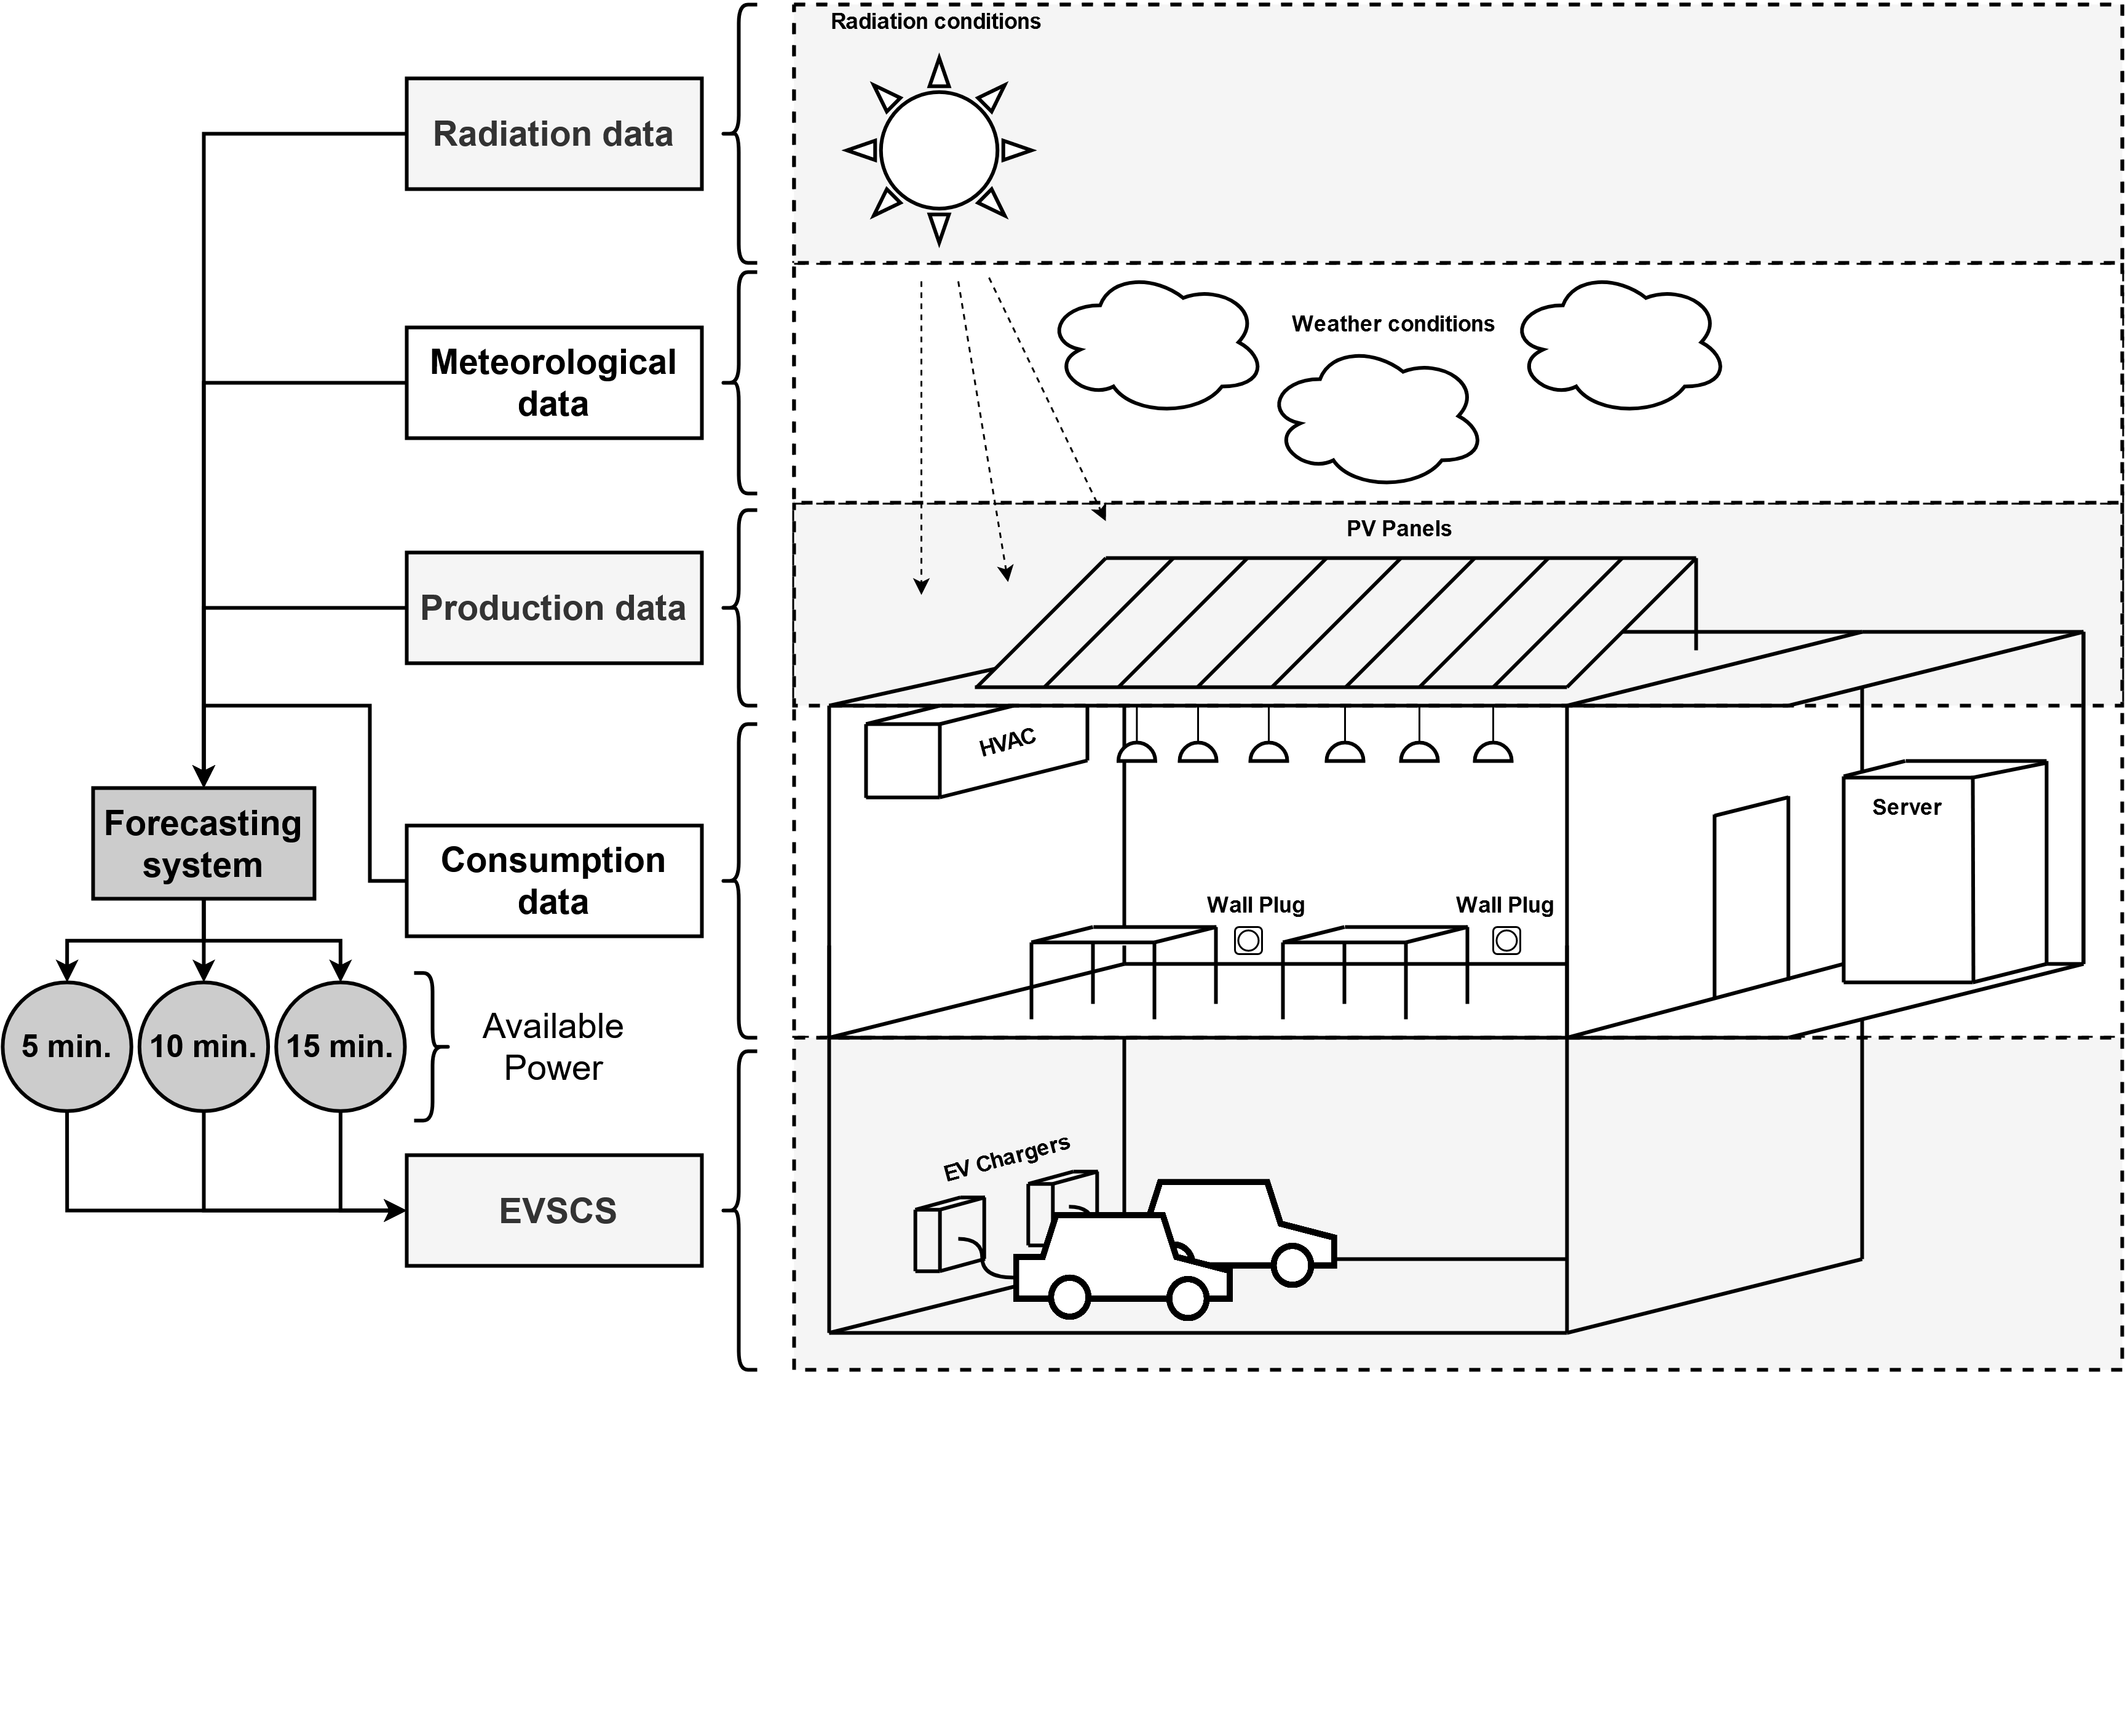
\includegraphics[width=1\textwidth]{Images/BUILDING.png}
    \caption{Building diagram.}
    \label{building}
    \end{center}
\end{figure}


A total of four datesets were used, with information on solar radiation and weather conditions of the area where the building is located, provided by \ac{FCUL}, and information regarding the power consumption and power production of the building, provided by \ac{EDP}. These datasets, besides having different dimensions and granularities, presented temporal gaps. It was then necessary to automate a data treatment process in which, regardless of the state in which the data is introduced in the system, it is treated and prepared to respect the structure that allows it to be used as input to the system. Next, six different models were developed: a Vanilla \ac{GRU}, a Vanilla \ac{LSTM}, a \ac{GRU} Encoder-Decoder, a \ac{LSTM} Encoder-Decoder, a \ac{1D CNN} - \ac{GRU} Encoder-Decoder and a \ac{1D CNN} - \ac{LSTM} Encoder-Decoder. Each one of the architectures has been built to, based on past available data, perform a forecast of the power available in the building in 5, 10 and 15 minutes. The performance of each of the architectures was evaluated and the best one was chosen. In addition, a variant of the already created models was tested and implemented, which consists of adding \ac{MCD} to the final models. The use of this methodology has the main purpose of generating random predictions and interpreting them as samples from a probabilistic distribution, which can not only help in determining the uncertainty of the model and its confidence intervals, but can also improve its performance as well. 

The result of this thesis is then a forecasting system capable of generating short-term forecasts of the available power of the building. The forecasts produced by the system are later provided to the \ac{EVCS}, that uses this information to optimize its decision process. The optimization process of the charging system is outside the scope of this thesis.

\section{Thesis outline}

This thesis is composed of five chapters in total. After this introduction in Chapter \ref{chap:intro}, Chapter \ref{chap:background} introduces the background and the work already developed in this field of research, both in a general aspect, where some of the most common models of \ac{ML} are detailed, and in a more specific aspect, where some of the work developed in building consumption forecasting is presented. In Chapter \ref{chap:architecture}, the case study proposed is introduced, and all the procedure taken into account, namely details concerning the building in question, selection of the variable to forecast, description of all the data processing carried out, description of the models proposed and implemented, environment in which the models were tested, and finally, the performance evaluation metrics applied. The results obtained are described in Chapter \ref{chap:results}. Lastly, Chapter \ref{chap:conclusion} presents the final conclusions of this work, as long as a brief description of what was accomplished.
% If Printing on DOUBLE SIDED pages, the second page should be white.
% Otherwise, comment the following command:
\cleardoublepage
%
%Chapter 2
% #############################################################################
% This is Chapter 2
% !TEX root = ../main.tex
% #############################################################################
% Change the Name of the Chapter i the following line
\fancychapter{Power availability forecast - Background and related work}
\cleardoublepage
% The following line allows to ref this chapter
\label{chap:background}

This chapter presents an overview of the fundamental and most commonly used models in \textit{Building Energy Consumption and Production Forecasting}, along with a revision of the related work in the field.

Before starting to dissect the history of predictive methodologies, one must consider that \textit{Time Series Forecasting} is an area with numerous utilities and that can be applied to several fields of research. Given the high energy consumption of buildings, the prediction of this factor can be the core basis for the development of intelligent systems, capable of optimizing resources and that contribute to a more economic and sustainable energy consumption profile.


\section{Methodologies\label{a}}

Over the past decades, numerous methods have been created to meet this challenge. The increase in the processing capacity of computers and the technological advance, in general, have been contributing to faster solutions, capable of obtaining more precise results in a shorter time span.

Currently, these approaches used for building energy simulation are categorized roughly as: (1) white-box based approaches, (2) grey-box based approaches and (3) black-box based approaches \cite{review2017}. 

White-box methods are based mostly on knowledge about the system. This type of methods requires knowledge of detailed information about the building in question, which makes it possible to obtain good accuracy in the forecasts obtained, but makes the models slow and complex to use.

Grey-box models are known to combine white-box models with data on past energy information from buildings, and apply statistical evaluations to predict future energy consumption.

Finally, the black-box methods are able to perform an assessment and produce a forecast of a building's energy consumption, based only on the building's statistical and historical information from the data, discarding the building's specific details (as is done in the other two methods). This allows this type of methods to produce results with better accuracy and at a much faster pace than the other alternatives. The main disadvantage is that in order to obtain a really useful and acceptable forecast, there must be a high amount of past data available to train, test and evaluate the model.

The work developed in this thesis aims to find a solution to the proposed problem through \ac{AI} and \ac{ML} techniques, which means that the focus of this work and respective research is based on black-box or, from now on, data-driven techniques.

\section{Data-driven prediction models\label{b}}

In 2020 there are numerous forecasting methodologies. Since data-driven techniques have been widely used for forecasting energy patterns, we will focus our research on these class of predictive techniques. In Figure \ref{datamodels}, there is a representation of some of the most common models applied in forecasting tasks.

\begin{figure}[h!]
    \centering
    \begin{center}
    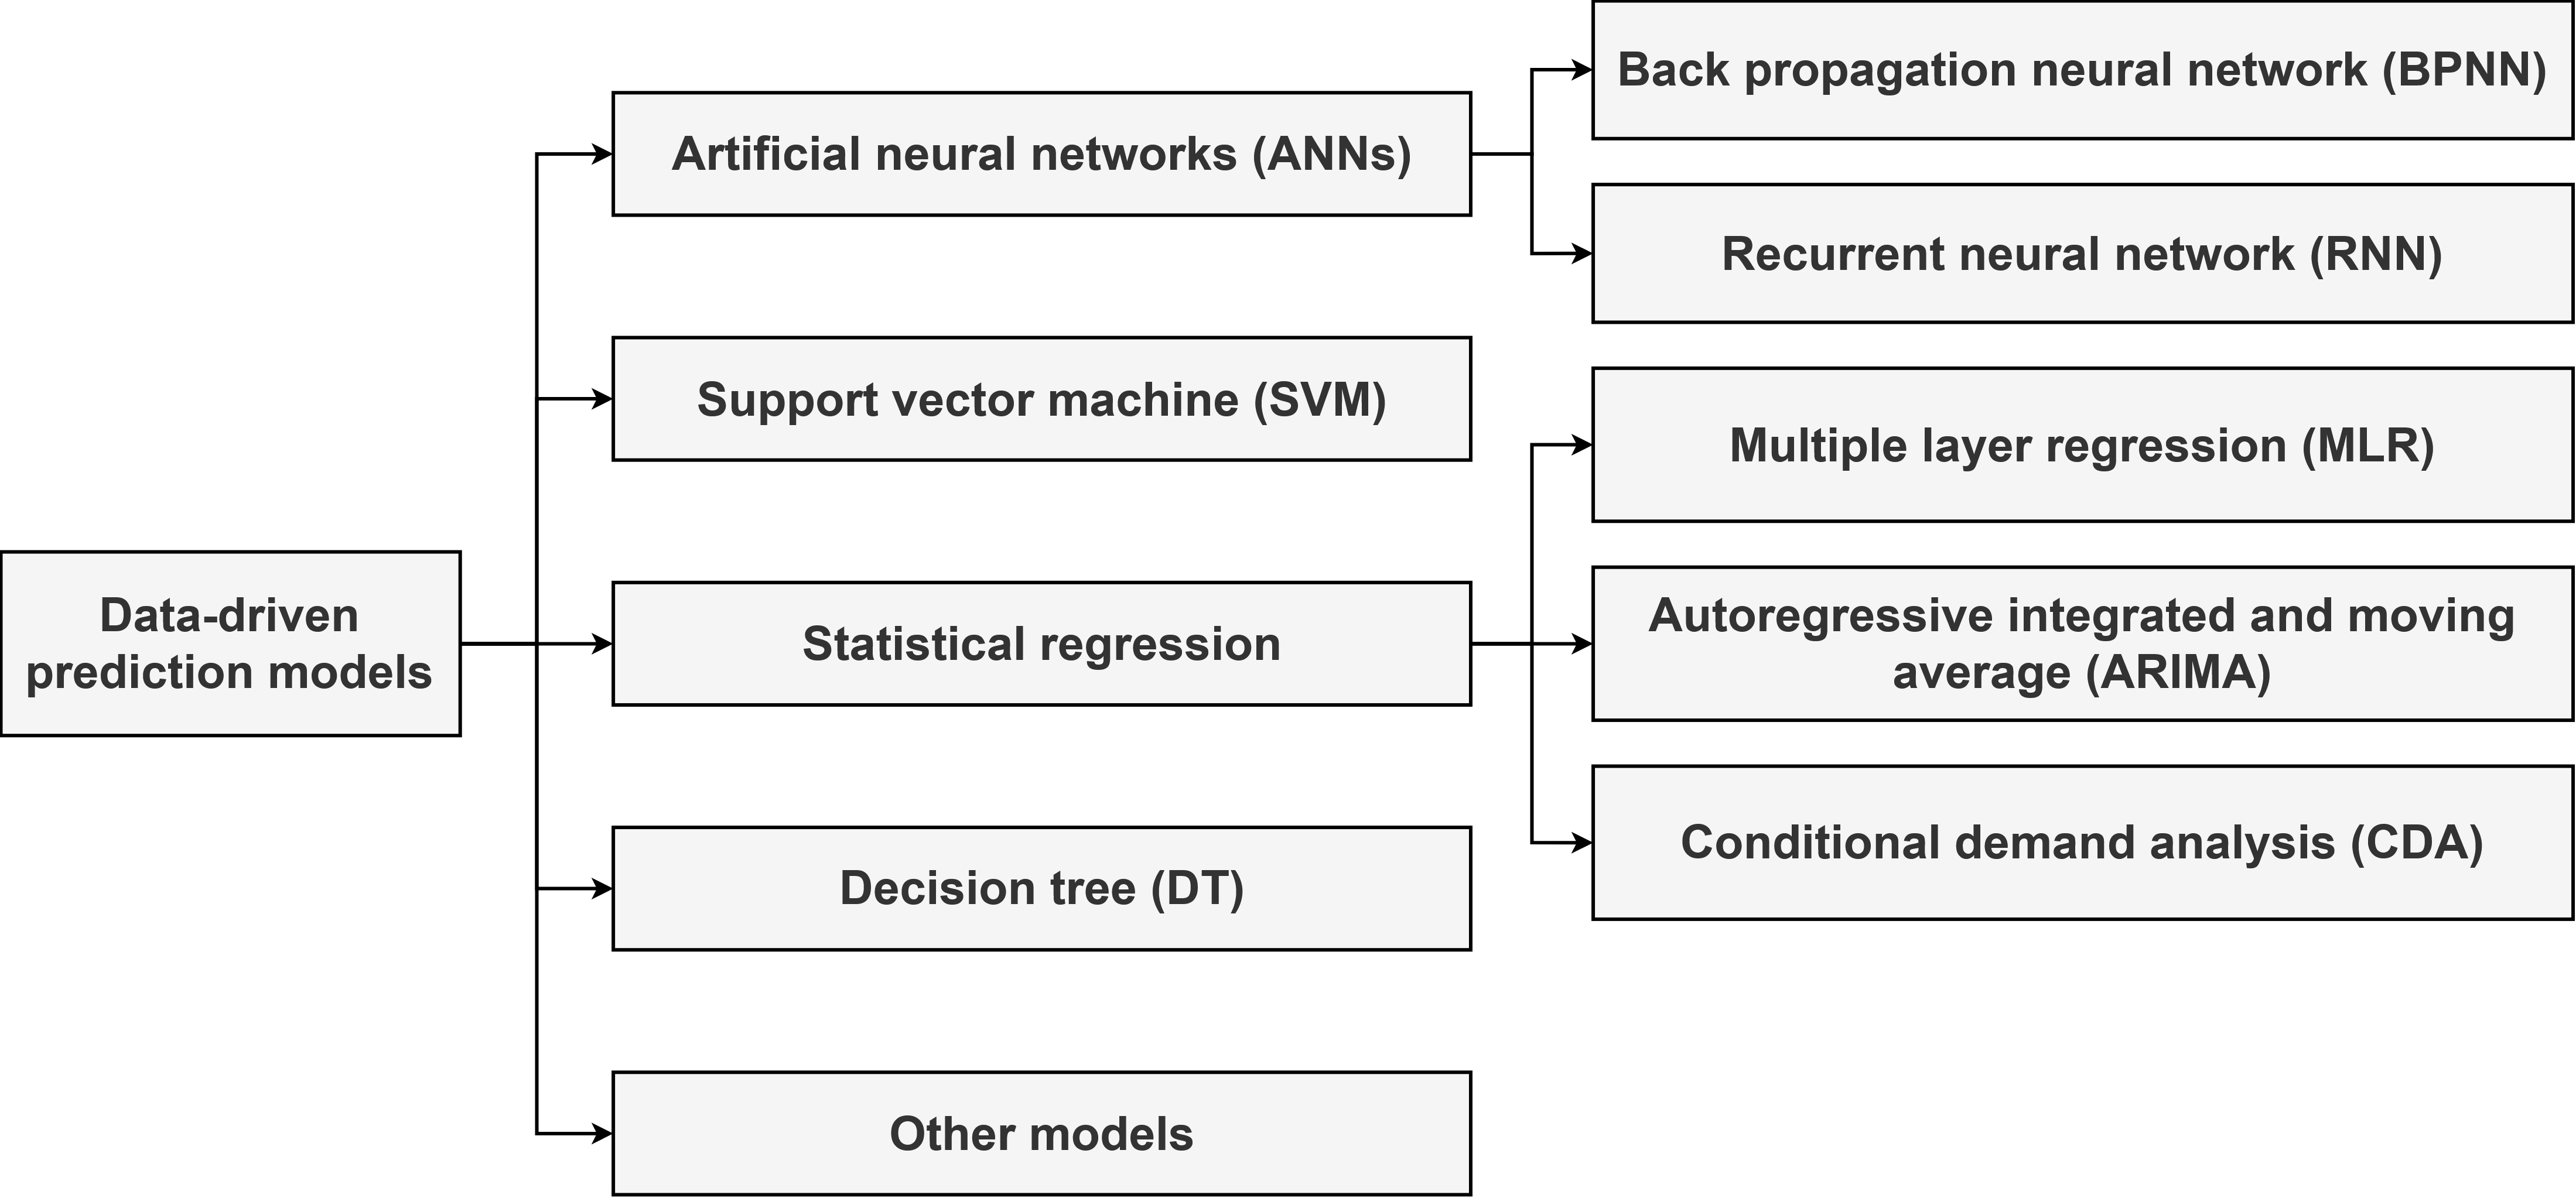
\includegraphics[width=1\textwidth]{Images/data-drive prediction models.png}
    \caption{Different data-driven models for forecasting tasks.}
    \label{datamodels}
    \end{center}
\end{figure}

To better understand how each of these methodologies works and how it can be used to solve the proposed problem, let us then move on to explain each of the main categories: \ac{ANN}, \ac{SVM}, Statistical regression, \ac{DT} and other models.


\subsection{Artificial neural networks (ANNs)}

Inspired by human brain architecture, a typical neural network consists of an interconnected group of artificial neurons, and it contains information using a connection list approach to computation \cite{ann1}. The application of this methodology has had enormous success when applied to nonlinear problems.

Structurally, \ac{ANN}s consist of a large number of neurons arrayed in different layers, connected with one another via connections \cite{review2017}. In Figure \ref{neuron}, it is possible to observe a representation of the basic computing element of an \ac{ANN}, the neuron. 
The neuron has a unique behavior, since it receives as input $I_i$ from other units or neurons, for example, and each one of these inputs, has associated a weight $w_i$, which changes its value based on the previous training of the network, in order to adjust the value of the input based on the proposed goal. The architecture of the neuron can be divided into two sections, in which the first adds products of weight coefficients and input signals, and the second section realizes the nonlinear function, called neuron activation function, i.e. $f(.)$. Therefore, the output function of the neuron is given by \cite{ann1}

\begin{equation}
   y = f(\sum_i w_i I_i + bias), 
   \label{tauequation}
\end{equation}

where the $bias$ is specific for each iteration and unit, and $f$ is the activation function. The most common transfer function is the sigmoid function \cite{ann1}

\begin{equation}
   f(x) = \frac{1}{1+e^{-x}}.
   \label{fequation}
\end{equation}

As the properties of common networks dictate, each neuron can serve as an input from the neuron in a next layer and so on.

In the Figure \ref{mlp} it is possible to see a scheme of a \ac{ANN}. It can be verified that it presents, as previously mentioned, a structure by layers. In this case, it is a \ac{FFNN} where the information circulates in only one direction, starting from the input layer, moving to the hidden layer, and ending in the output layer. 



\begin{figure}[h!]
\captionsetup[subfigure]{position=b}
\centering
\subcaptionbox{\label{neuron}}{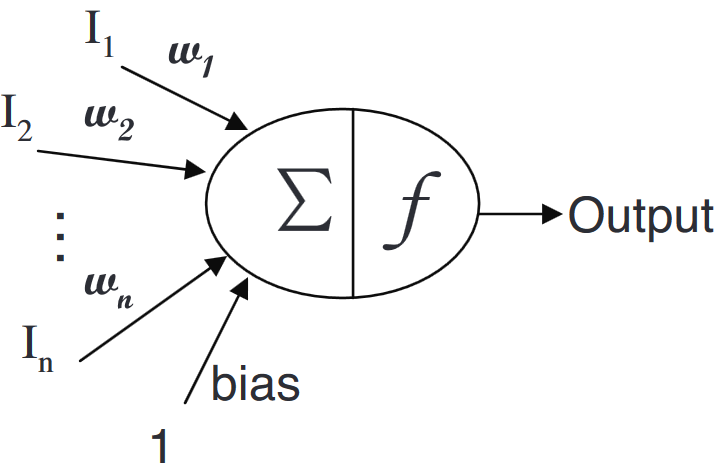
\includegraphics[width=.4\linewidth]{Images/neuron.PNG}}
\hspace{0.05\textwidth}
\subcaptionbox{ \label{mlp}}{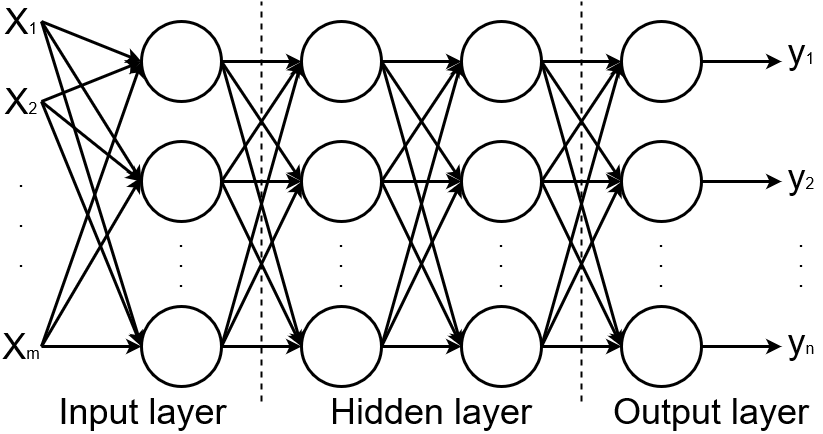
\includegraphics[width=.49\linewidth]{Images/ANN.png}}
\caption{Example of one neuron a) and a multi-layer perceptron b).}
\end{figure}

This is a very simple representation, but there are more complex models such as \ac{BPNN} and \ac{RNN}, which should be introduced.

\subsubsection{Back-propagation neutral network (BPNN)}
The \ac{BPNN} was developed by Rumelhart \cite{bpnn0}, is one of the most commonly used methods super-vised learning models of ANN. According to Goh \cite{bpnn}, in \ac{BPNN}s, the mathematical relation-ships between the various variables are not specified. Instead, they learn from the examples fed to them. In addition, they can generalize correct responses that only broadly resemble the data in the learning phase. Figure \ref{bpnn} shows the architecture of a \ac{BPNN} where the neural network computes the error of the output for each iteration, and then propagates this information as a negative feedback to tune the incoming connection weight and bias. This manipulation offers flexibility to modify the output error to a minimum, which  improves the accuracy of the \ac{ANN} calculation \cite{review2017}. To minimize the output error, the gradient descent method is used to compute the weight of each neuron and to adjusts the weight of interconnections. At the output of each node, the error is defined as

\begin{equation}
   E = \frac{1}{2}\sum_k(T_k-A_k)^2,
   \label{EBPNN}
\end{equation}

where $T_k$ is the actual value of the output of the neuron, $A_k$ denotes the predicted value of the output of the neuron and $k$ is the output neuron. 

\subsubsection{Recurrent neutral network (RNN)}

The \ac{RNN}, on the other hand, implies that the output of each neuron serves as input for the previous layer processing units, or even the for the same layer itself, in order to identify temporal patterns. This design makes this family of networks ideal for working with time series data-sets \cite{rnn1},\cite{rnn2},\cite{rnn3}, without shuffling, being the type of models that is applied more regularly in time-series forecasting problems.

In Figure \ref{rnn} is a representation of the architecture of a generalized \ac{RNN}, where it is possible to verify the existence of feedback loops in their recurrent layer. This helps them keep information in 'memory' for an extended period \cite{rnn4}.

\begin{figure}[h!]
\captionsetup[subfigure]{position=b}
\centering
\label{fig:Mould}
\subcaptionbox{\label{bpnn}}{
\includegraphics[width=.4\linewidth]{Images/bpnn.png}}
\hspace{0.05\textwidth}
\subcaptionbox{ \label{rnn}}{
\includegraphics[width=.4\linewidth]{Images/rnn.png}}
\caption{a) Back-propagation neural network (BPNN)  and b) Recurrent neutral network (RNN).}
\end{figure}

Although these models present a good behavior in temporal data prediction and modeling, it is difficult to train vanilla \ac{RNN}s whose data have a great temporal dependence. This is due to the loss function gradient that decays exponentially over time (which is referred to as the gradient vanishing problem)\cite{rnn4}. To combat this problem, new types of \ac{RNN}s have been developed, such as \ac{LSTM} and \ac{GRU}, whose behavior will be explained in a later chapter, which have been having an enormous success in predicting time-series patterns. 


\subsection{Support vector machine (SVM)}

Another very popular Machine Learning methodology is the \ac{SVM}. Introduced by Cortes, Corinna and Vapnik, Vladimir in 1995 \cite{svm1}, \ac{SVM}s are widely applied to estimate the relationship nonlinear inputs and real-value outputs continuous in time. \ac{SVR} is a specific type of \ac{SVM} used for regressions and it is an algorithm that allows the user to choose how tolerant he is with errors. The tolerance can be controlled both through an acceptable error margin($\varepsilon$) or through tuning an acceptable error rate.
Function \ref{svmdec} is constructed by performing some training process with historical data. The whole operation of a \ac{SVR} is based on the creation of a decision function $F(x_i)$

\begin{equation}
   F(x_i) = \langle w, \varphi(x_i) \rangle + b,
   \label{svmdec}
\end{equation}

where $\langle\cdot,\cdot\rangle$ represents the inner product, $w$ represents weight defined in $R^N$, $\varphi(x_i)$ represents the non-liner mapping of the input space to a high-dimensional feature space and b represents the bias\cite{svm2}. $w$ and $b$ are unknown variables, that are estimated by minimizing the regularized risk function \cite{svm2}. According to Magoules F. \cite{ann1}, the regularized risk can be solved using its dual form, introducing Lagrangian $L$

\begin{equation}
\begin{split}
       L & := \frac{1}{2}\parallel w \parallel^2 + c \sum_{i=1}^{n}(\xi_i + \xi_i^*) - \sum_{i=1}^{n}(\eta_i\xi_i + \eta_i^*\xi_i^*) - \sum_{i=1}^{n}a_i(\varepsilon + \xi_i - y_i- \langle w, \varphi(x_i) \rangle - b) \\ 
         & - \sum_{i=1}^{n}a_i^*(\varepsilon + \xi_i^* - y_i- \langle w, \varphi(x_i) \rangle - b),
\end{split}
\end{equation}

where $\{a_i, a_i^*, \eta_i, \eta_i^*\geq 0\}$ are the Lagrangian Multiplier, $\parallel w \parallel$ is the Euclidean norm, ${{\xi_i,\xi_i^*\geq 0}}$ are two slack variables to copy with some infeasible optimization constraints\cite{review2017}. Another constant $c \geq 0$ determines the trade-off between the training error (over-fitting) and model flatness (under-fitting)\cite{review2017}. 
It is important to mention that the Lagrange multipliers ($\eta_i = c - a_i$, $\eta_i^* = c-a_i^*$) are all independent. $\{a_i, a_i^*\}$ can be determined by the corresponding dual optimization \cite{ann1}

\begin{equation}
\begin{split}
       & Maximize \  W(a_i, a_i^*) = -\frac{1}{2}\sum_{i=1}^{n}\sum_{j=1}^{n}(a_i-a_i^*)(a_j-a_j^*)(\varphi(x_i)\cdot \varphi(x_j) + \\
       & \sum_{j=1}^{n}(a_i-a_i^*)y_i - \varepsilon \sum_{j=1}^{n}(a_i+a_i^*),\\
       & subject \  to \begin{cases} \sum_{j=1}^{n}(a_i-a_i^*) = 0 \\ a_i, a_i^* \in [0,c]. \end{cases} 
\end{split}
\end{equation}

After computing $a_i, a_i^*$, one can write $w$ as a function of $\{ a_i, a_i^*. x_i\}_{i=1}^n$. One can then infer the decision function for \ac{SVR}
\begin{equation}
      F(x) = \sum_{x_i \in SV} (a_i-a_i^*)K(x, x_i)+b , 
      \label{ioi}
\end{equation}
 where $K(x, x_i) = \varphi(x)\cdot\varphi(x_i)$. In \ac{ML}, one can call this function the \ac{SVR} kernel function, that which varies according to the intended final application. Another aspect to consider is that the sum presented in the equation \ref{ioi} does not include all the inputs, only the support vectors. Moreover, the bias $b$ is calculated based on these support vectors

\begin{equation}
\begin{split}
       b = & \frac{1}{N_1} \Bigg\{ \sum_{a_i \in (o,C)} \Bigg[ Y_i-\sum_{x_k\in SV}(a_j-a_j^*)K(x_i, x_j) - \varepsilon \Bigg] + \\
           & \sum_{a^*_j \in (o,C)}\Bigg[Y_i-\sum_{x_k\in SV}(a_j-a_j^*)K(x_i, x_j) - \varepsilon\Bigg] \Bigg\},
\end{split}
\end{equation}
 where $N_1$ is the number of support vectors. After the decision function, i.e., Eq.\ref{svmdec}, is fully defined by the training process, the \ac{SVR} model created is ready to compute predictions for a new input\cite{review2017}.
 

\subsection{Statistical regression}

The third family of methods is the statistical regression family. This is a set of methods quite famous for their simplicity of use in the area of forecasting building consumption. This solution is based on the attempt to map a relationship between the outputs and the inputs that contribute to the behavior of the system. The statistical regression methodologies create a probabilistic model capable of relating different variables, which contribute to an output given by 
\begin{equation}
       Y_i = \alpha_i + \beta_1 x_{i,1} + \beta_2 x_{i,2} + ... + \beta_m x_{i,m} + \varepsilon_i,\quad if \  multiple,
\label{multi}
\end{equation}
or
\begin{equation}
       Y_i = \tilde{\alpha_i} + \tilde{\beta_1} x_{i,1} + \tilde{\beta_2} x_{i,2}^2 + ... + \tilde{\beta_m} x_{i,m}^m + \varepsilon_i,\quad if \  polynomial,
\label{poly}
\end{equation}

where $x_i$ represents the input, $\varepsilon_i$ represents a random normally distributed error, and  $\alpha_i, \tilde{\alpha_i}, \beta_j\  and\  \tilde{\beta_j}\ (j=1,...,m)$ are the parameters to be estimated. To give an example, let's focus on multiple linear regression, E.q. \ref{multi}, in which the estimates of all the parameters where computed using the \ac{LS} method. Let's also introduce the notion of \ac{SSE} as

\begin{equation}
       SSE = \sum_{i=1}^n (y_i-A_i-B_1 x_{i,1} - B_2 x_{i,2} - ... - B_m x_{i,m})_i^2,
\label{SSE}
\end{equation}
 where $A_i$ and $B_j(j\ =\ 1,...m)$ are the corresponding \ac{LS} estimates of $\alpha_i$, $\beta_j(j\ =\ 1,...m)$ in E.q.\ref{multi} \cite{review2017}. Using this method, one should proceed to the minimization of the SSE which originates $m+1$ equations, in which each one of them presents a partial derivative of the \ac{SSE} in order to $A_i$ and $B_j(j=1,...,m)$ which should be equal to zero. It is through these equations that it is possible to determine the parameters $A_i$ and $B_j(j=1,...,m)$ that refer to the respective historical data. You can then write the equation
 
\begin{equation}
       y_i = A_i + B_1 x_{i,1} +  B_2 x_{i,2} + ... + B_m x_{i,m},
\label{y_i}
\end{equation}

known as the predictive equation with the estimated parameters in the form of multiple linear regression.
 
This model has become in forecasting medium to long term patterns and is widely used with that purpose. As a negative point, in order to make a good forecast, a large amount of data is needed, which makes this model limited by temporal constraints, which means that it is not a good model to use when there is a small amount of time available to run the model. As far as short term forecasting is concerned, it has been found that it presents worse results than models such as \ac{ANN}s and \ac{SVM}s.

\subsection{Decision tress (DT)}

\ac{DT} models \cite{dt1}, structurally present a tree inspired architecture consisting of a graph that has a root node and a set of branch nodes. In this architecture, the system inputs are inserted in the root node, where they are divided successively in different groups as they advance in the tree, based on a predetermined division criterion. This split data is then propagated to sub-nodes as branches from the root node.

The inner nodes of the tree subsequently apply divisions of the sub-data into new sub-data. The end nodes or leaf nodes that serve as output nodes. 
This type of methodologies can also be applied to the concrete case of energy forecasts of buildings. In the Figure \ref{dt} one can see an example where the range of consumption values is divided into hierarchical groups and the model classifies in the future the consumption of the building associating it with one of these groups.


\begin{figure}[h!]
    \centering
    \begin{center}
    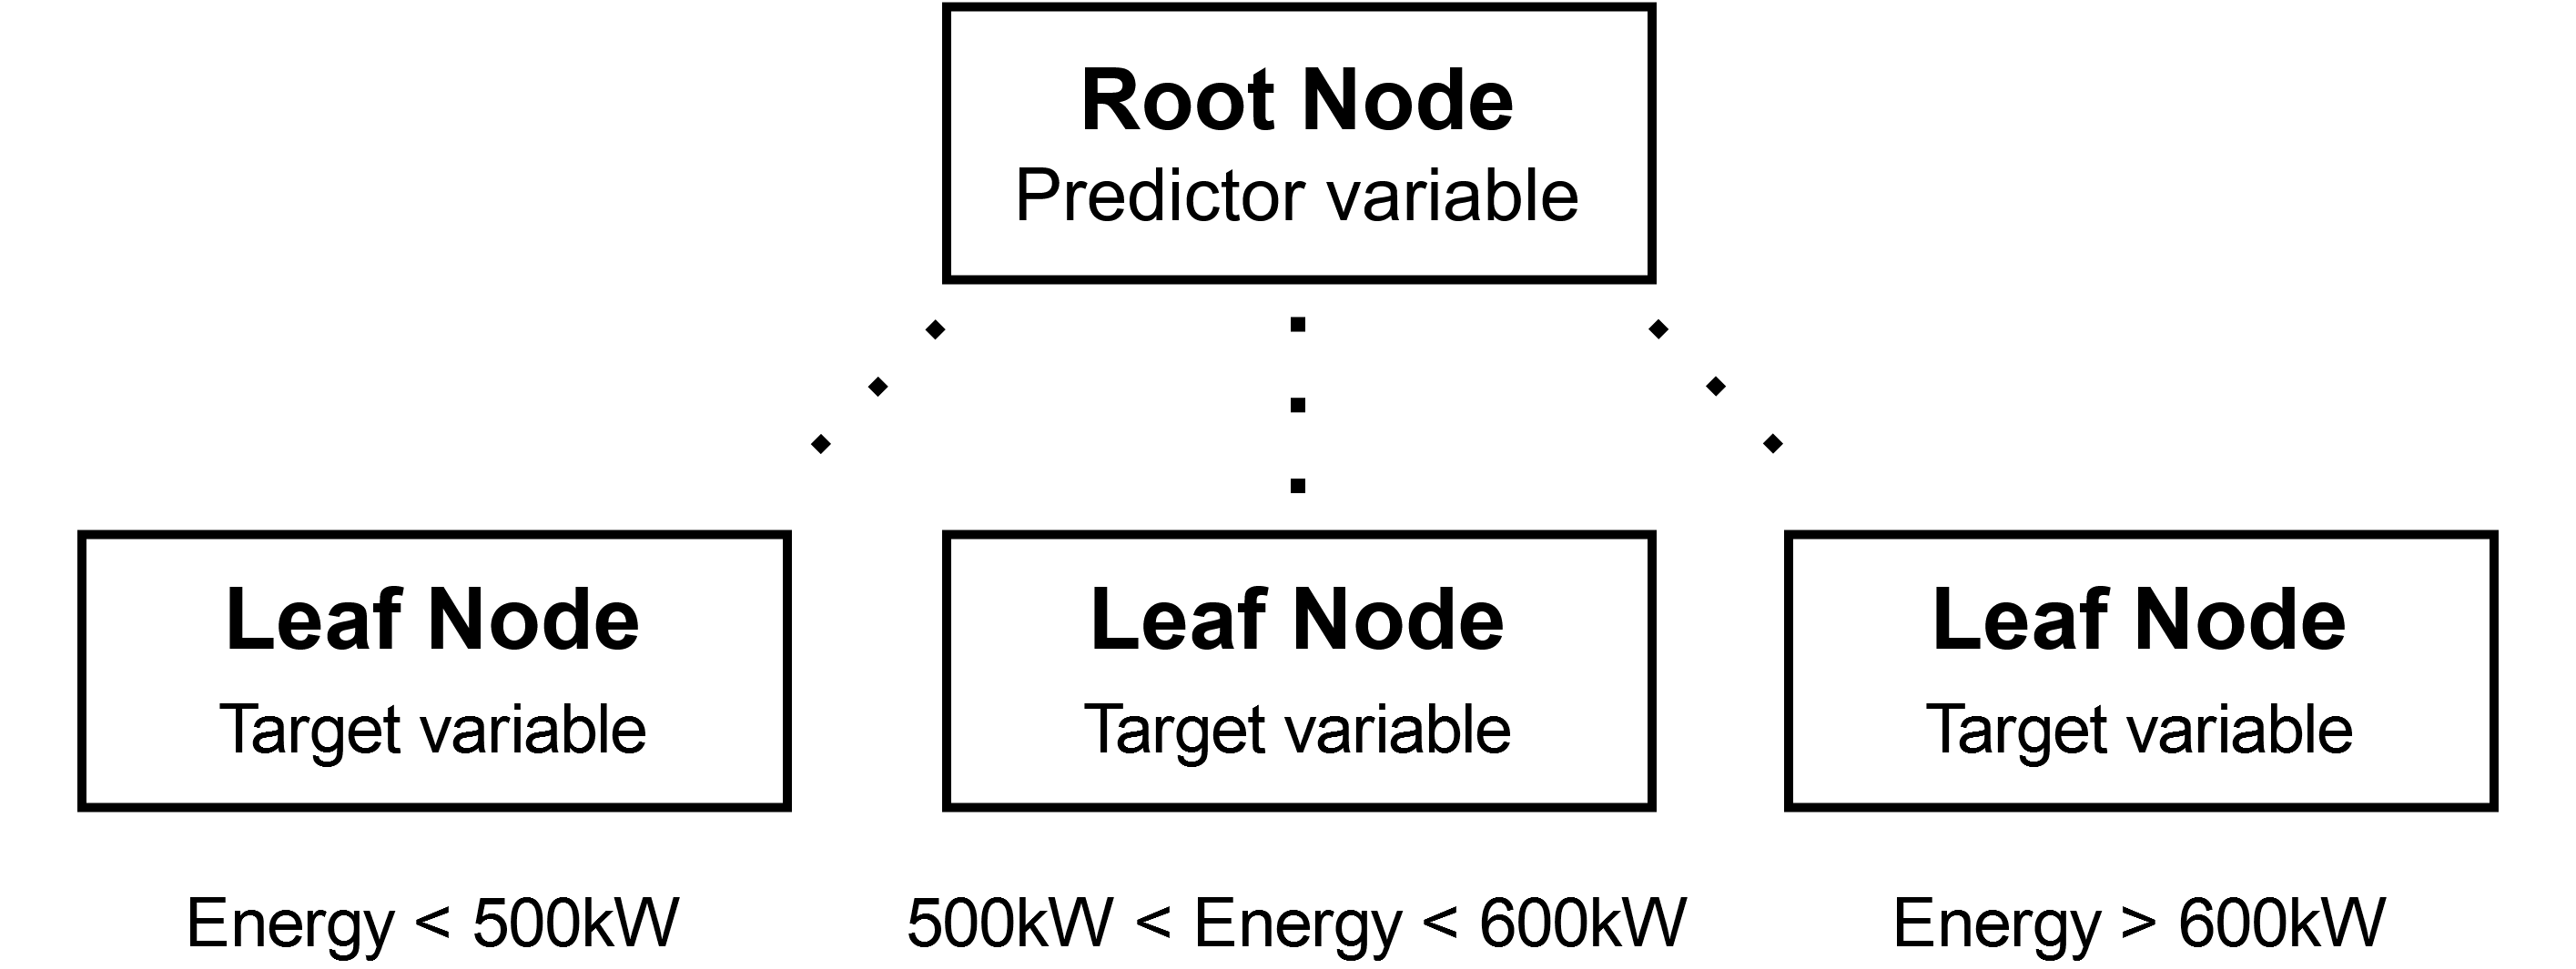
\includegraphics[width=0.6\textwidth]{Images/DT.png}
    \caption{Decision tree example.}
    \label{dt}
    \end{center}
\end{figure}

A relevant concept when it comes to the use of \ac{DT}s, is the concept of entropy
\begin{equation}
       E=\sum_{i=1}^n -P_i\log_2P_i,
\label{entropy}
\end{equation}

where $E$ is the information entropy, $n$ is the number of different target values and $P_i$ is the probability of a dataset taking the $i^{th}$ target value. This parameter is used to calculate the gain ratio of the \ac{DT}.

The biggest advantage of using this type of methodologies is the fact that it is a simple method to implement and does not require extensive computational knowledge to put it to work. Compared to other data-driven methods, the main disadvantage is that the targets or categories defined for leaf nodes are based on assumptions. In the example in Figure \ref{dt}, the previously defined energy ranges are those because there is an expectation that the future values fit into one of the categories. This limitation can sometimes generate errors or deviations from the real values. The architecture of this model is also in itself a limitation because it does not present a good performance for nonlinear data \cite{dt2}.


\section{Data-driven prediction models applied to building energy forecasting \label{c}}

Both the architectural and the technical specifications of a building, such as the type of glass used, geographical position, etc., have a huge impact on the way this kind of structures manage their production and energy consumption. 

Electricity consumption has increased in the commercial sector in the last fifteen years.  In commercial buildings, annual energy consumption per square meter of floor space is over 200 kW h, with air conditioning being the final application that consume the most energy within a building\cite{pie_1}. In Figure \ref{buildingenergy} \cite{pie_1}, a graph with the distribution of energy consumption in commercial buildings, in several groups, can be found.


\begin{figure}[h!]
    \centering
    \begin{center}
    \begin{tikzpicture}
    \pie[color={black!10, black!20, black!30, black!40}, text=pin]
        {4/Refrigeration, 
         4/Cooking,
         6/Lighting,
         7/Electronics,
         7/Others,
         9/Space cooling,
         18/Water heating,
         45/Space heating}
         
    \end{tikzpicture}
    \caption{End use wise energy consumption in commercial buildings.}
    \label{buildingenergy}
    \end{center}
\end{figure}


As can be seen in Figure \ref{buildingenergy}, space cooling, space heating and water heating represent more than 70\% of a building's energy consumption, which presents a direct correlation with  the number of people present in the building at each moment. Thus, it can be seen in the Figure \ref{consumption} that in office buildings, the energy consumption presents a behavior that respects a certain trend, which concerns the employees' working hours, vacation days, etc.

The ability to build models that take these factors into consideration and that can predict what the future energy consumption of the building will be, is a competence that enables not only the creation of more sustainable solutions, but also the design of optimization models for the use of these sources of consumption, limiting their use when necessary.

According to \cite{reviewtsf}, factors such as such as occupancy schedule, weather conditions, thermal properties of building materials, complex interactions of the energy systems like \ac{HVAC} and lighting etc have a huge impact in the energy behavior of a building. 

Giving all the necessary building specifications to take into account when applying white and grey-box techniques, it is quite complex to build a model capable of simulating the behavior of the building. In this sense, data-driven methods appear as a viable alternative. These techniques are based on past recorded data, and try to build a future model based on past observed energy patterns. Techniques that use past data to develop a model to predict future behaviour, often fall under the category of \ac{ML} and have been actively applied to building energy forecasting studies in the last two decades. With this notion in mind, let's then look at some concrete cases where the models described above have been applied in forecasting energy consumption of buildings.

The use of a simple prediction model has been common practice for many years, but with the progress of technology and computational capacity, the combination of several prediction models has become more and more common. In this regard, it is important to mention two very relevant model architectures, Ensemble models and Hybrid models. 

Ensemble models consist of models composed of several different machine learning techniques in parallel, where the different models work separately. Each of the models gets a certain answer, and then there is a voting system that determines the final forecast. 

Hybrid models are also models composed of several different machine learning techniques, but which work in series, where the result obtained by a certain model is introduced as input to the next model. In this type of architecture the two models work together to obtain a single output (there is no voting).

These two model typologies allow to obtain not only a better predictive performance than the one that would have been obtained using the models separately, but also more flexibility in model construction.

In Appendix B, Table \ref{table1}, the reader can find a table with all the applications mentioned in this section, the type of building involved, the input data, the output data, the size of the dataset and the type of model of models used.


According to \cite{ann1}, \ac{ANN}s are the most widely used artificial intelligence models in the application of building energy prediction. D. Datta et al. \cite{annr1} started, in 2000, to apply \ac{BPNN}s to forecast the energy consumption of a supermarket and since then, different \ac{BPNN}s models have been widely used in forecasting energy consumption of different types of buildings, such as office buildings, commercial buildings, residential buildings, etc. \cite{annr4}, \cite{annr9}, \cite{annr13}, \cite{annr14}, \cite{annr17} and \cite{annr19}. Kalogirou \cite{annr2} also explores the integration of \ac{ANN}s for predicting the energy consumption of a building that has integrated solar panels by applying a combination of \ac{RNN}s with a \ac{BPNN} model to predict the energy consumption of a seasonal holiday house. Yang et al. \cite{annr3} predicted one day ahead electric consumption of an office building by experimenting a sliding window \ac{ANN} methodology and accumulative \ac{ANN} methodology. Both Yezioro et al. \cite{annr5}, and Yokoyama et al. \cite{annr7} developed systems to forecast more specific indicators, eating energy consumption cooling energy consumption of a building, by using \ac{BPNN}s, as well as Ekici et al. \cite{annr6}, just for heating and Cheng-wen et al. \cite{annr8}, just for cooling. Later another methodology for forecasting energy consumption of buildings was also tested, which applies a \ac{BPNN} with multiple outputs \cite{annr10} so that one could choose the best option from among the results obtained, and Li et el.\cite{annr12} proposed two hybrid models, the \ac{iPSO-ANN} which adjusts the weights of the neural network, and the \ac{GA-ANN} model.
On the other hand, Deb et el. \cite{annr15}, Shi et el. \cite{annr16}, Hossen et el. \cite{annr18} and Gasparin et el. \cite{annr21},  have also used \ac{RNN}s to predict energy consumption of buildings, both offices and buildings as well as residential buildings and have concluded that this type of models presents a high accuracy, based on the use and knowledge of past consumption data of the buildings in question. Ruiz et el. \cite{annr22} introduced a methodology to predict future energy consumption using \ac{NAR} and the \ac{NARX} , respectively.
Finally, Deb et et. \cite{annr20}, used \ac{BPNN}s to create energy saving systems associated with the use of \ac{HVAC} in office buildings.
Li et el. \cite{annr24} developed a new hybrid method called teaching learning based optimization \ac{TLBO-ANN} to optimize \ac{ANN}’s parameters in order to forecast two actual building energy consumption. Ruiz et el. \cite{annr25} was also able to predict the energy consumption of multiple university buildings by applying Elman neural networks with evolutive optimization in 2018. Fan et el. \cite{annr26} compared \ac{RNN}s, \ac{LSTM}s and \ac{GRU}s while predicting the energy consumption of an educational building and \cite{annr27}, \cite{annr28} and \cite{annr29} are examples of hybrid models combining several types or \ac{ANN}s with the same purpose. 


In 2005, Dong et el. \cite{svm2} applied \ac{SVM}s to predict the energy consumption of a commercial building in tropical region. Then, in 2009, Li et el. \cite{svmr1} also applied \ac{SVM}s to predict the hourly cooling load of a building. Later, in 2010, Paudel et el. \cite{svm3} implemented an architecture with two parallel \ac{SVM}s to predict eating demand and electrical load of several office buildings and in 2017, et el. \cite{svmr7}, used again \ac{SVM}s to predict the consumption of a residential building. In 2010 Xuemei et el. \cite{svmr2}, introduced a \ac{FSVM} and fuzzy c-mean clustering for predicting the cooling load of Zhongkai university scientific building, and concluded that \ac{FSVM} has better effectiveness and efficiency of the learning and prediction in contrast to others, such as classical \ac{SVM}s. Edwards et el. \cite{svmr3} developed a case study where he implemented a \ac{SVR} to predict hourly electrical consumption of a residential building, and Zhang et el. \cite{svmr4} combined also \ac{SVR}s with a differential evolution optimization technique for the same purpose. Ma also applied et el. \cite{svmr5} \ac{SVM}s to tackle the same problem in China, and concluded that \ac{SVM} model forecasts agree well with the statistic values in all the seven zones of the country tested, as well as with the whole nation's data. Lastly, in 2019, Zhong et el. \cite{svmr6}, also applied \ac{SVR}s for building energy consumption prediction of an office building and concluded that "The energy consumption prediction obtained by applying the proposed models to a real office building can provide an accurate energy consumption scheduling plan for the power system, which has practical significance for energy planning, management, and conservation". \ac{SVM}s are models that can obtain good results for forecasting building's energy profiles because they can deal with non-linear relations by transforming them into linear relations in a higher dimension. On the other hand, \cite{svm3}, \cite{svm2} and \cite{svm5} identified that \ac{SVM} is a slow model for large scale problems.
 
In 2015 Fumo et el. \cite{regression0} applied both simple and multiple regression analysis in a case study regarding residential buildings. Later in 2018, Ahmad et el. \cite{dt0} applied both DTs and regression models for predicting the consumption behaviour of multiple buildings.

There are also studies that evaluate different models by applying them to the same case study. In 2009, et el. \cite{svmr0}, Setiawan compared several methods when performing load forecasting, and concluded that the \ac{SVR} model could outperform the \ac{BPNN}s, but simpler models such as linear regression could produce similar accuracy results in a much faster way. Seyedzadeh et el. \cite{other2}, also tested different models for predicting energy consumption of buildings and concluded that \ac{GBRT} provide the most accurate predictions. However, when the data was simple (in term of input variables and size), \ac{SVM} was proven to be the best choice because of simplicity and the speed of calculations. Lastly, Fan et el. \cite{other1}, compared the results when manipulating the features of a \ac{GAN}, which helped to bridge the knowledge gap between deep learning and building operations. 

Besides the models presented, there are also other data-driven models that were applied with the same purpose. Although are not used so regularly, less common models have been gaining some relevance in recent years, namely due to the significant increase in computing power available. Most of these methods are also a sub-category of the methods presented above. 

\ac{ANFIS}, is model that has an architecture similar to an artificial neural network that was developed in the early 1990s \cite{anfis1}, \cite{anfis2}. This methodology complements \ac{ANN}s with fuzzy logic principles \cite{anfis3}, which allows defining if-then rules to approximate non-linear functions that led \cite{anfis4} to classify \ac{ANFIS} as a universal estimator.


Wang et el. \cite{rf0} used a \ac{RF} technique, compared it to the most common approaches such as \ac{SVM}s and tried to demonstrate that RF is also a good choice when trying to predict building energy consumption.

Other method \ac{ELM} consists of feed-forward neural networks where the parameters of the hidden nodes don't need to be tuned. These hidden nodes can be randomly assigned, or can be inherited from their ancestors without being changed. Usually, the output weights of the hidden nodes are learned in a single step, which resembles the linear learning process. According to Guang-Bin Huang \cite{elm1}, the advantage of these models is their capability of producing a good generalization performance and learn in a faster pace than networks trained using back-propagation, and according to \cite{elm2}, \cite{elm3} and \cite{elm4}, these models have the capability to outperform support vector machines in both classification and regression applications.



\section{Conclusion}

In this section we introduce the main topics related to power availability forecast and the work done in this area. In the section \ref{a}, we started by doing a brief introduction of the different types of predictive methodologies and we explained the difference between each of them.

Then, in section \ref{b}, we have distinguished the different data-driven models and introduced theoretically the most common models in this branch.

Lastly, in the section \ref{c} we presented some of the most important applications of data-driven models for forecasting energy consumption of buildings, specifically.

% If Printing on DOUBLE SIDED pages, the second page should be white.
% Otherwise, comment the following command:
\cleardoublepage
%
%Chapter 3
% #############################################################################
% This is Chapter 3
% !TEX root = ../main.tex
% #############################################################################
% Change the Name of the Chapter i the following line
\fancychapter{Case Study}
\cleardoublepage
% The following line allows to ref this chapter
\label{chap:architecture}


In the last chapter we presented some of the most important models in the literature regarding the prediction of power consumption in buildings. In this chapter, we present in detail the challenge proposed by \ac{EDP}, and the procedure carried out throughout the development of this thesis.

\section{Problem statement and framework}\label{chap3:sec:problem_statement}

The proposed objective for this work is to create a system capable of computing predictions regarding the available power in a building, 5, 10 and 15 minutes ahead. Since all the experiment is directly related to the behavior of a specific building, it makes sense to present the building and its characteristics. Then, it is important to describe the whole procedure carried out to be able to produce those three forecasts.

\section{The building}\label{chap3:sec:building}

The building provided by \ac{EDP} for the development o this research has a total useful area of 39,801$m^2$ distributed in 5 major categories, office area, parking area, technical area, gymnasium area and bar, with the first two areas representing 89\% of the total area of the building. In Figure \ref{consedp} there is a diagram that shows the distribution of energy consumption by type of final use in each area of the building, for the year of 2016.

\begin{figure}[h!]
    \centering
    \begin{center}
    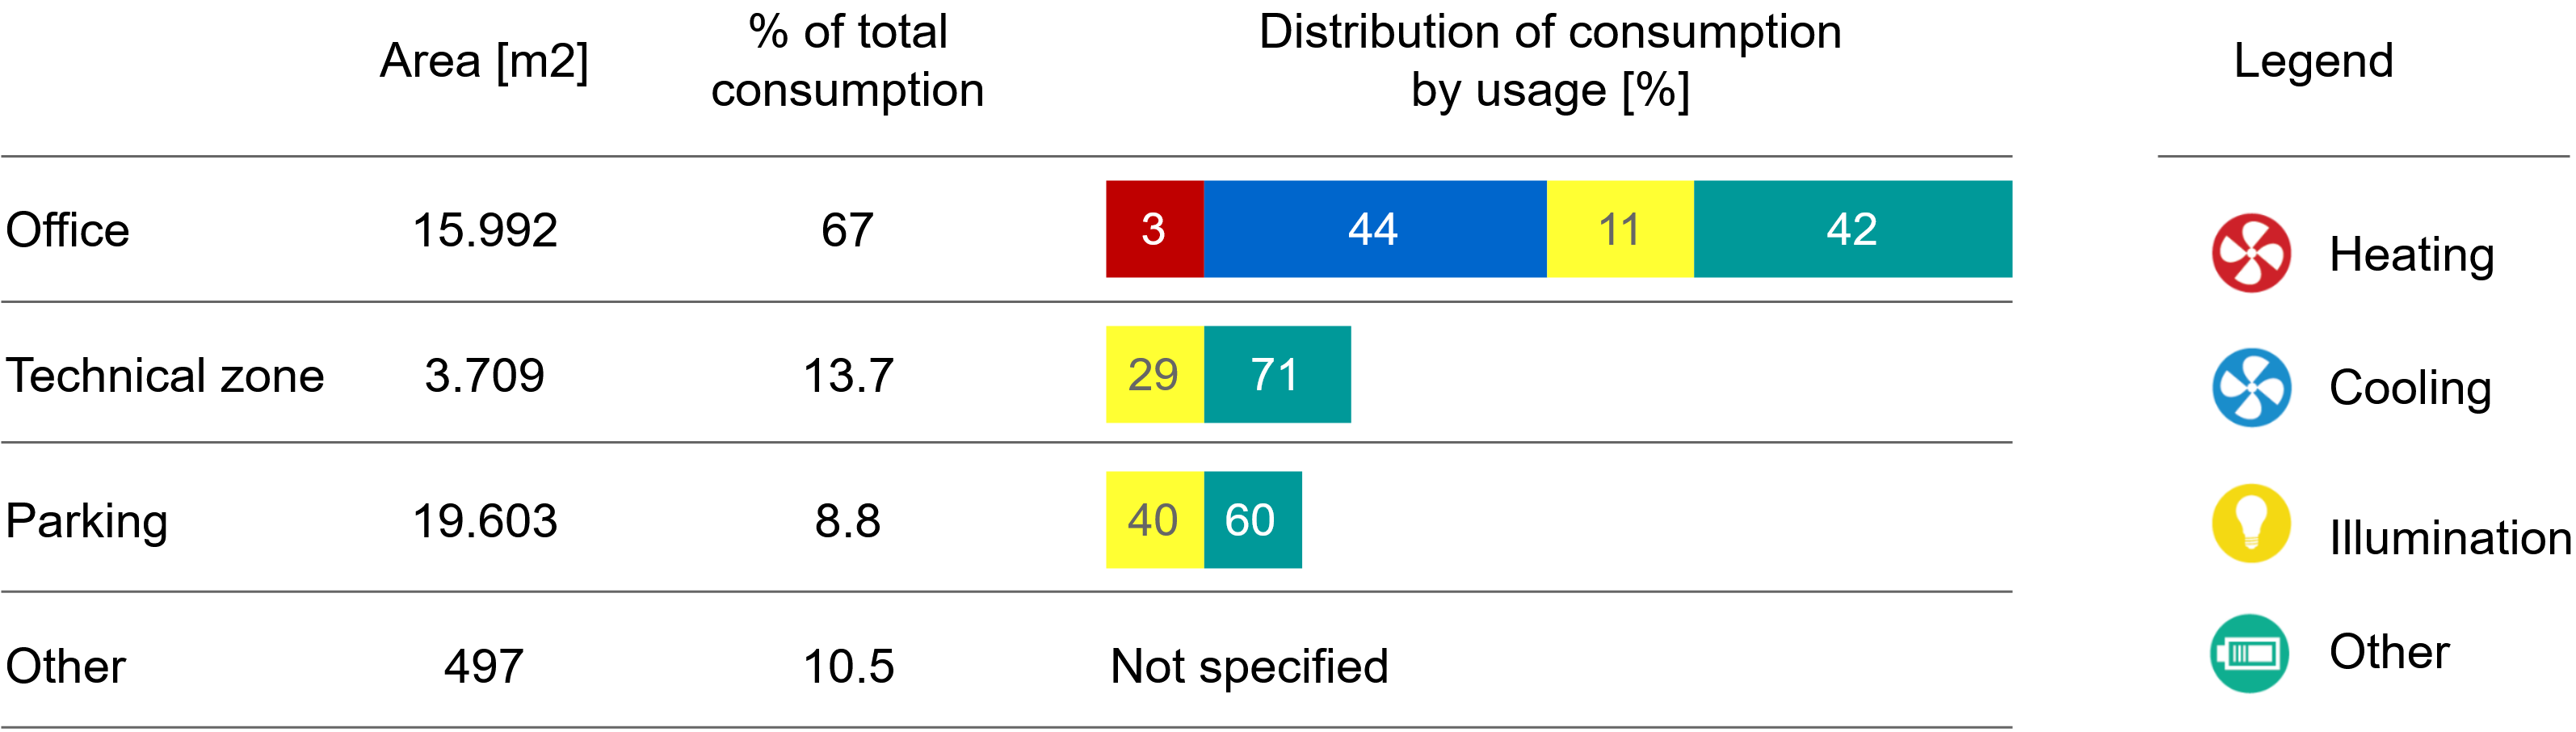
\includegraphics[width=1\textwidth]{Images/ConsumoEDP.png}
    \caption{Energy consumption for the building typology(s) with the highest consumption (2016).}
    \label{consedp}
    \end{center}
\end{figure}
In Figure \ref{consedp}, it can be seen that the \ac{HVAC} system represents almost 50\% of the consumption in the office zone. The use of the \ac{HVAC} system is directly related to the external weather conditions. In contrast to the commercial buildings referenced in section \ref{c}, since 44\% of the consumption is connected to the office cooling process, it can be deduced that in the region where this building is located, in warmer years, the consumption of the office area is higher, contributing to an increase in the total consumption of the building. It can also be seen that only 11\% of consumption is due to the lighting of the office area. On the other hand, 42\% of the consumption in the office area is made up of all other factors such as energy plugs. The technical zones represent about 14\% of the total consumption of the building although they represent a small portion of the total area of the building. Most of the consumption performed in these areas is identified as "other" and concerns servers and technical material of the high energy consumption, hence the enormous representativeness of these zones in the total consumption of the building. Parking lots also represent a significant portion of the total consumption of the building. It should be noted that 60\% of consumption is also identified as "other". This portion mainly concerns the electric car charging procedure, that is carried out in the building's garage, managed by the \ac{EVCS}, addressed in Chapter \ref{chap:intro}. This system consists of a total of 13 charging stations for \ac{EV}s, and falls into the category of controllable consumption, i.e., the system can control the power used in vehicle charging, based on the priority level of each vehicle (such as the percentage of full battery charged), and the total power available in the building. The contribution of this thesis falls exactly in this category. Although the system has instantaneous information of the available power state in the building, it would be of great use to have information regarding the future state of available power. In this sense, the work developed in this dissertation aims to respond to this need, contributing to the optimization of the current system.

Modeling energy consumption behaviour and identifying patterns can be crucial both to minimize power usage, and to develop new methodologies to optimize resources. Figure \ref{consumption} illustrates the energy consumption profile of \ac{EDP}'s building in Lisbon, Portugal, during the month of February 2020. The profile illustrated in Figure \ref{consumption} shows a movement that one can identify as a trend. The data presented provides power consumption details for 4 weeks and 4 weekends. The behaviour of the profile tends to be cyclical with a 7 day period. 
\begin{figure}[h!]
    \centering
    \begin{center}
    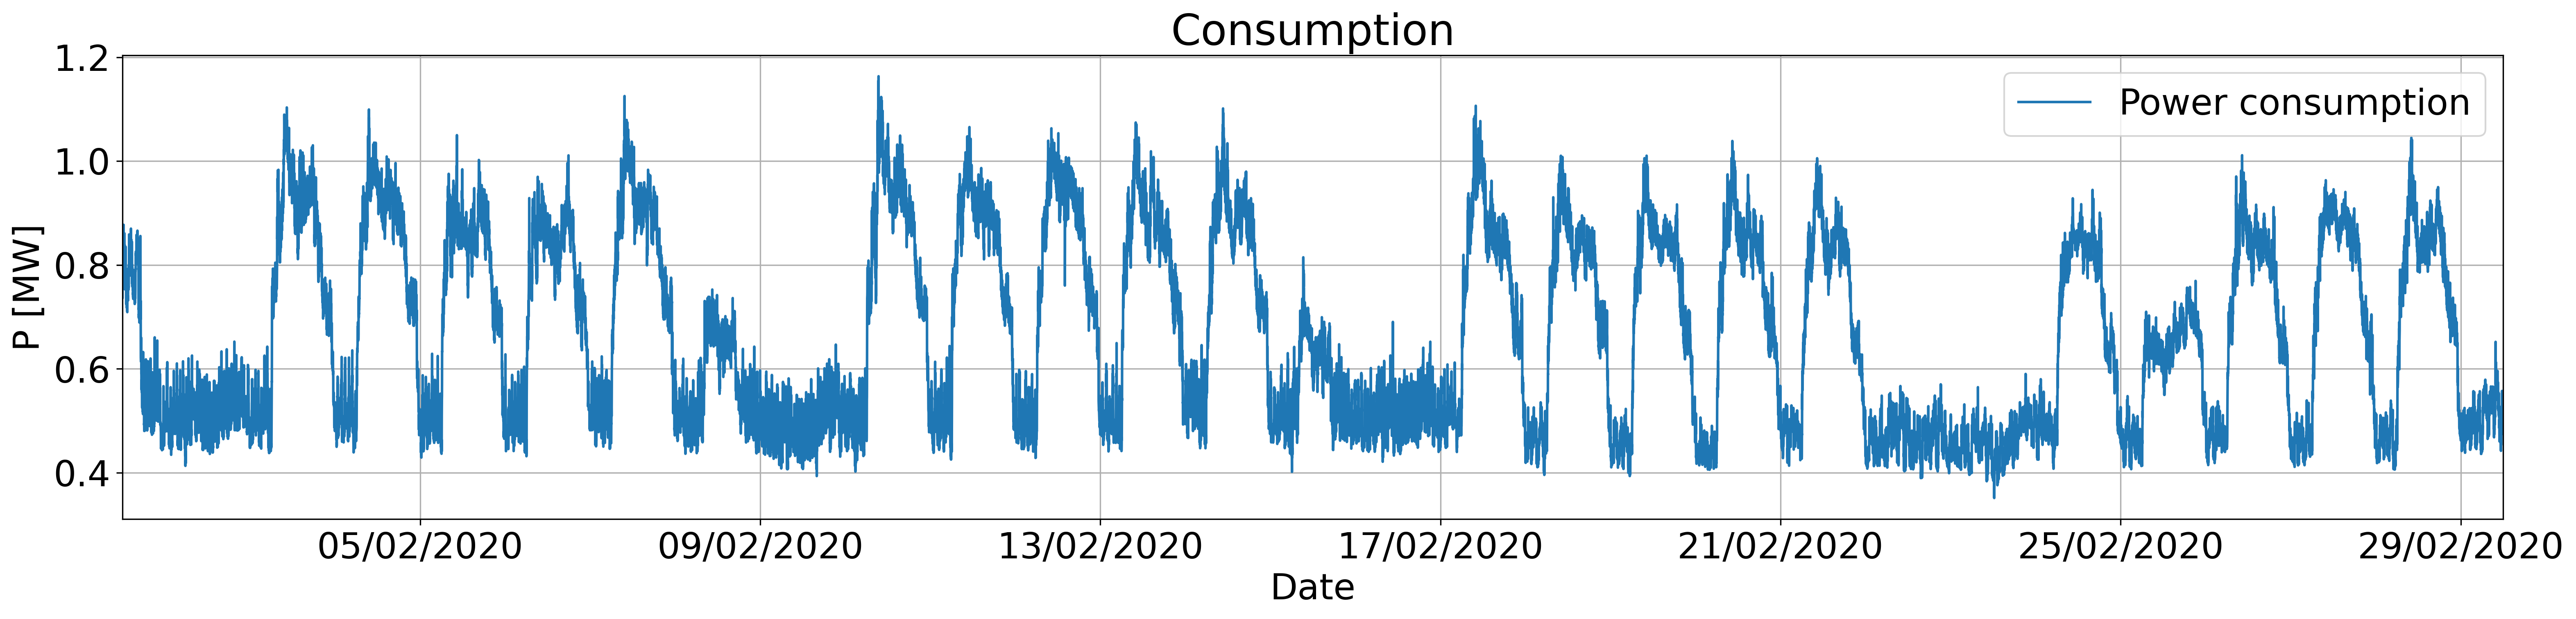
\includegraphics[width=1\textwidth]{Images/power_consumption.png}
    \caption{EDP's building's a) consumption.}
    \label{consumption}
    \end{center}
\end{figure}


Variables that present a trend are more easily examined since it is sometimes possible to associate a cause with their cyclical behavior. By identifying this cause, it becomes not only easier to control its current behavior, but also to predict its future behavior. 

%Power consumption forecasting for buildings is a well know area of research. According to \cite{CivilEU}, Energy consumption forecasting plays a significant role in plans to improve energy performance, save energy and reduce the hazardous environmental impact. Moreover, forecasting also plays a vital role in decision-making and future planning which rely on accurate forecasting results. The ability to predict the available power of any building has many interesting utilities. 

As far as power production is concerned, the building is equipped with a total of 500$m^2$ of \ac{PV} panels area on its roof. The efficiency of the installed panels is around 15$\%$, which represents a total of 70 kWp (kilowatt "peak") of solar generation. Although this kind of production is not controllable, since it depends solely on weather conditions, there are several relationships that can be established by having access to meteorological information. The increase in production generated by the \ac{PV} panels, directly represents an increase in the available power to consume. This factor then becomes an important indicator in the development of any forecasting system, since its behaviour directly influences the the amount of power available to charge \ac{EV}s. In Figure \ref{production}, one may see the power production profile for the same building and time-interval as Figure \ref{consumption}. The \ac{PV} production behaviour is also cyclical but presents a daily period due to the fact that solar radiation is not influenced by the occupancy rate of the building, so it has no direct relation with the day of the week, but with the hour of the day instead.

\begin{figure}[h!]
    \centering
    \begin{center}
    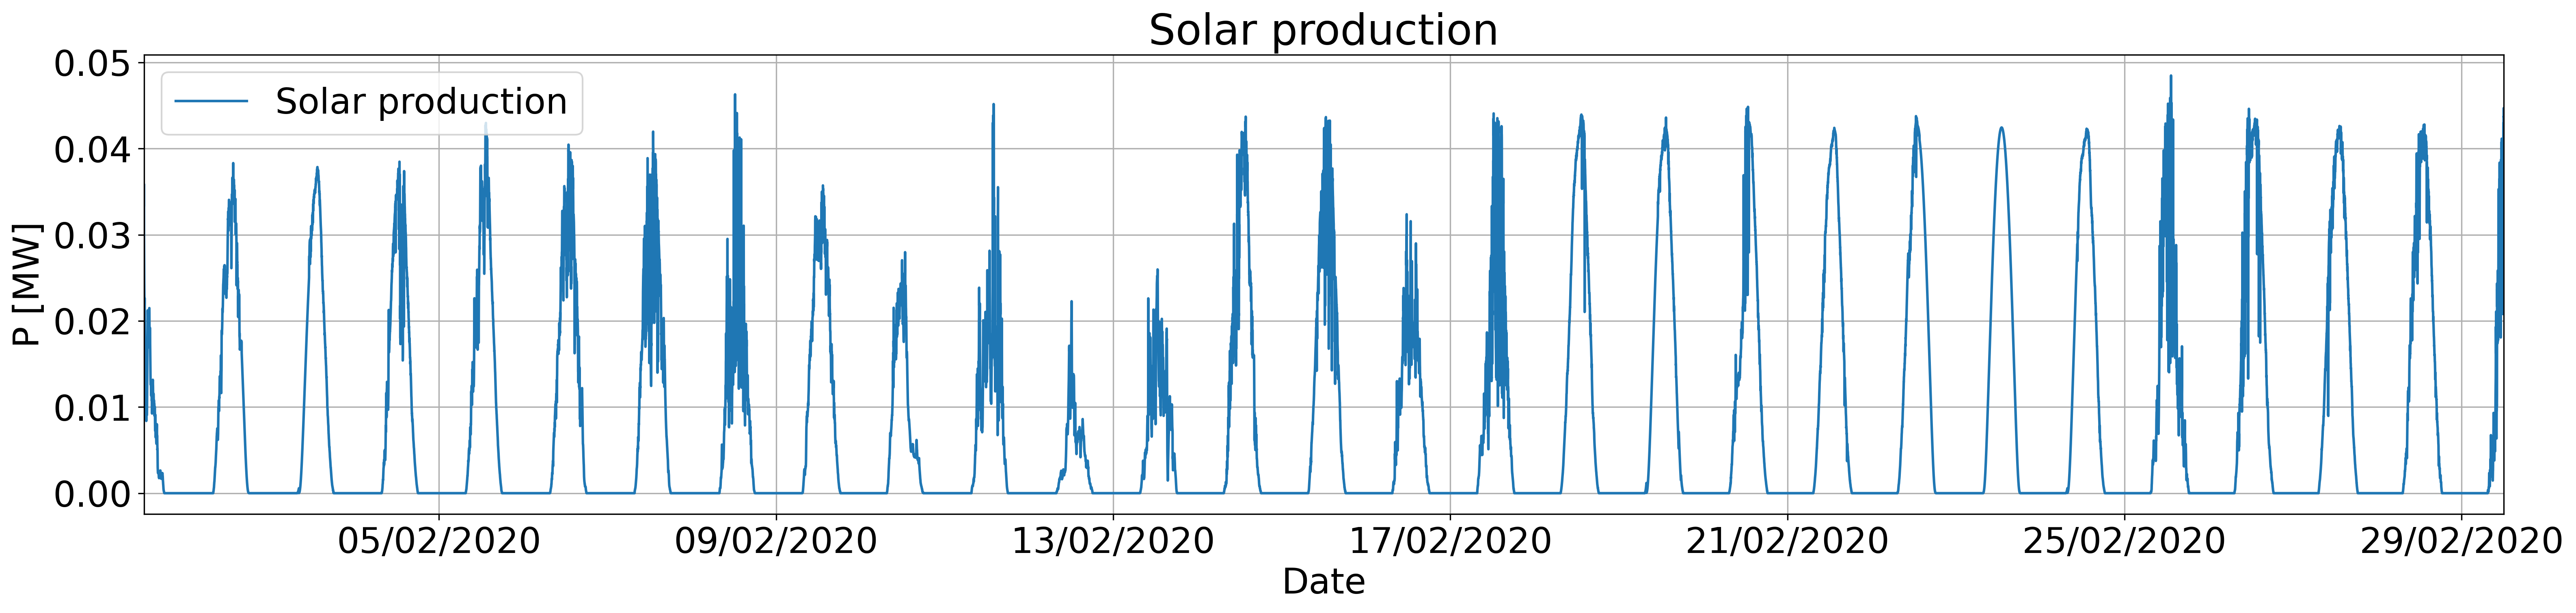
\includegraphics[width=1\textwidth]{Images/power_production.png}
    \caption{EDP's building's a) production.}
    \label{production}
    \end{center}
\end{figure}


Both power consumption and power production are vital information to have in order to predict power available at each time in the building. With this information, there are multiple innovative ideas that can be implemented with the goal of having a more sustainable and power-optimized building.

\section{Proposed variable to predict}\label{chap3:sec:variable_to_predict}

The available power is a key factor because it is the indicator provided to the \ac{EVCS} that enables it to proceed with the optimization of the distribution of the available power by the \ac{EV}s present in the building's garage, which need to be charged.

The power available is not a measured variable, it is a calculated variable. When it comes to computing it, one question then arises: Should one compute the available power and then predict it, or should one predict both consumed power and produced solar power, and just then perform the calculations to find the available power? Figure \ref{avsol} represents two possible solutions for this problem. The first solution consists in creating a model that has as input, besides the other variables, two variables: consumption power and solar production. This model will have as output a forecast for these two variables, and only then is the available power calculated. The second solution is to compute the available power before inputting the data into the model, which causes a reduction in the number of inputs and outputs in the model. 

\begin{figure}[h!]
    \centering
    \begin{center}
    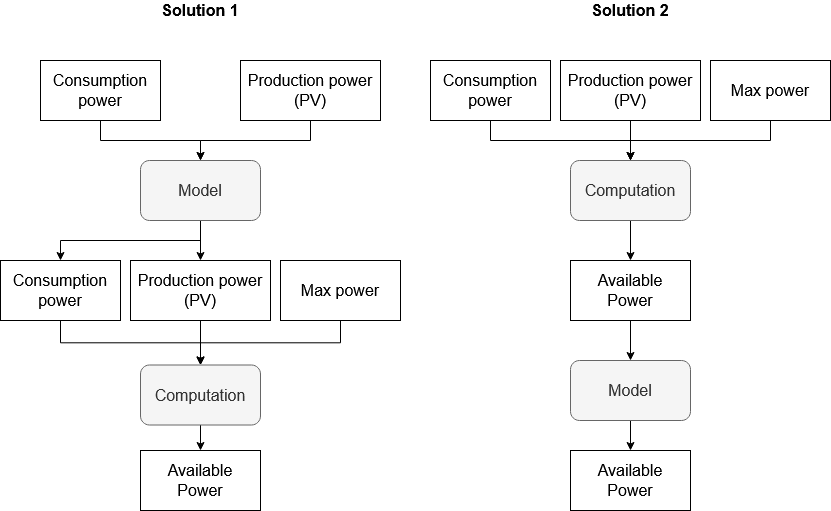
\includegraphics[width=1\textwidth]{Images/Available.png}
    \caption{Model solutions.}
    \label{avsol}
    \end{center}
\end{figure}

Comparing the two proposed hypotheses, solution 1 presents the advantage of predicting two different variables allowing better data manipulation, offering more flexibility. Since the model produces separate results for the consumption and production variables, the amount of possible uses for this data is greater than the amount of possibilities provided by solution 2. On the other hand, solution 2 presents, first of all, the advantage of having a much simpler architecture which makes the user's work easier, and secondly, the main advantage is that it requires the model to predict only one variable instead of two. This factor is quite relevant, namely regarding the time it takes the system to produce forecasts, and also the computational capacity that is required from the hardware to allow the prediction of two variables simultaneously. The prediction of two variables with the same model also has the disadvantage of making it difficult to evaluate the behavior of the proposed solution, since a specific model can be very good for predicting one of the variables and very bad for the other. 
Taking all these factors into account, the second approach was then chosen, which facilitates the user's work, allows to produce results more quickly, and facilitates the process of choosing a model that produces a good solution for a single variable.


In Figure \ref{Max_cons_prod}, the reader may see the graph for the power profile of \ac{EDP}’s building, for February 2020, where the blue line is the power consumption of the building, the orange line the solar power production, and the red line the power of the electrical grid made available to this specific building.


\begin{figure}[h!]
    \captionsetup[subfigure]{position=b}
    \centering
    \label{fig:ap}
    \subcaptionbox{\label{Max_cons_prod}}{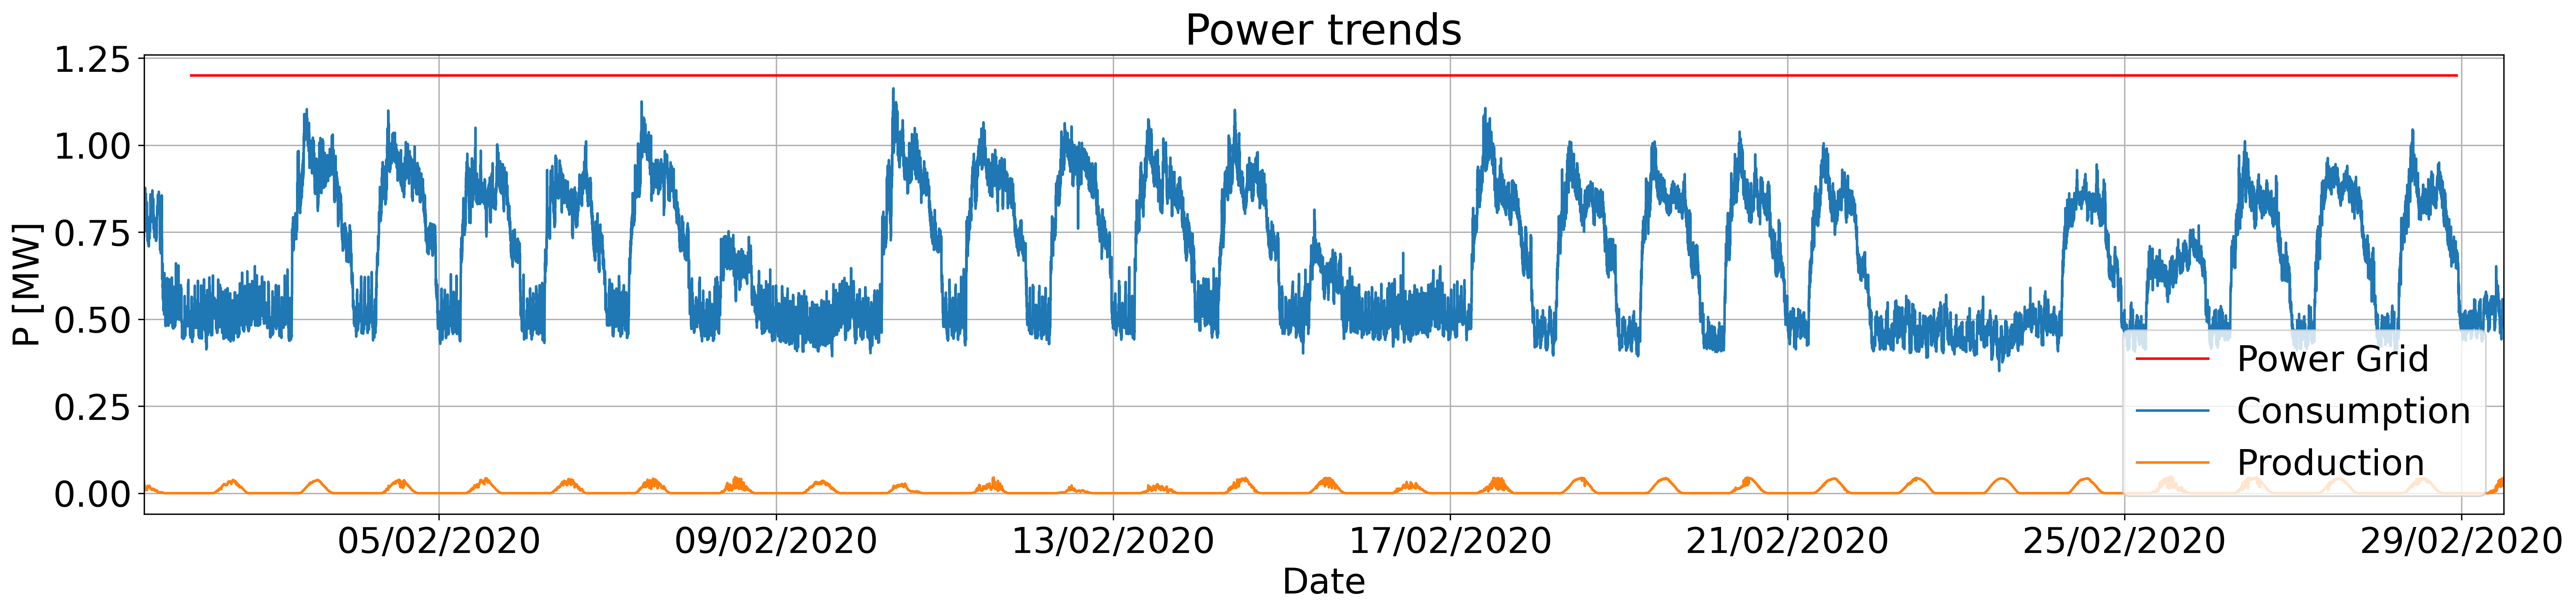
\includegraphics[width=1\linewidth]{Images/Max_cons_prod.png}}
    \subcaptionbox{ \label{available_power}}{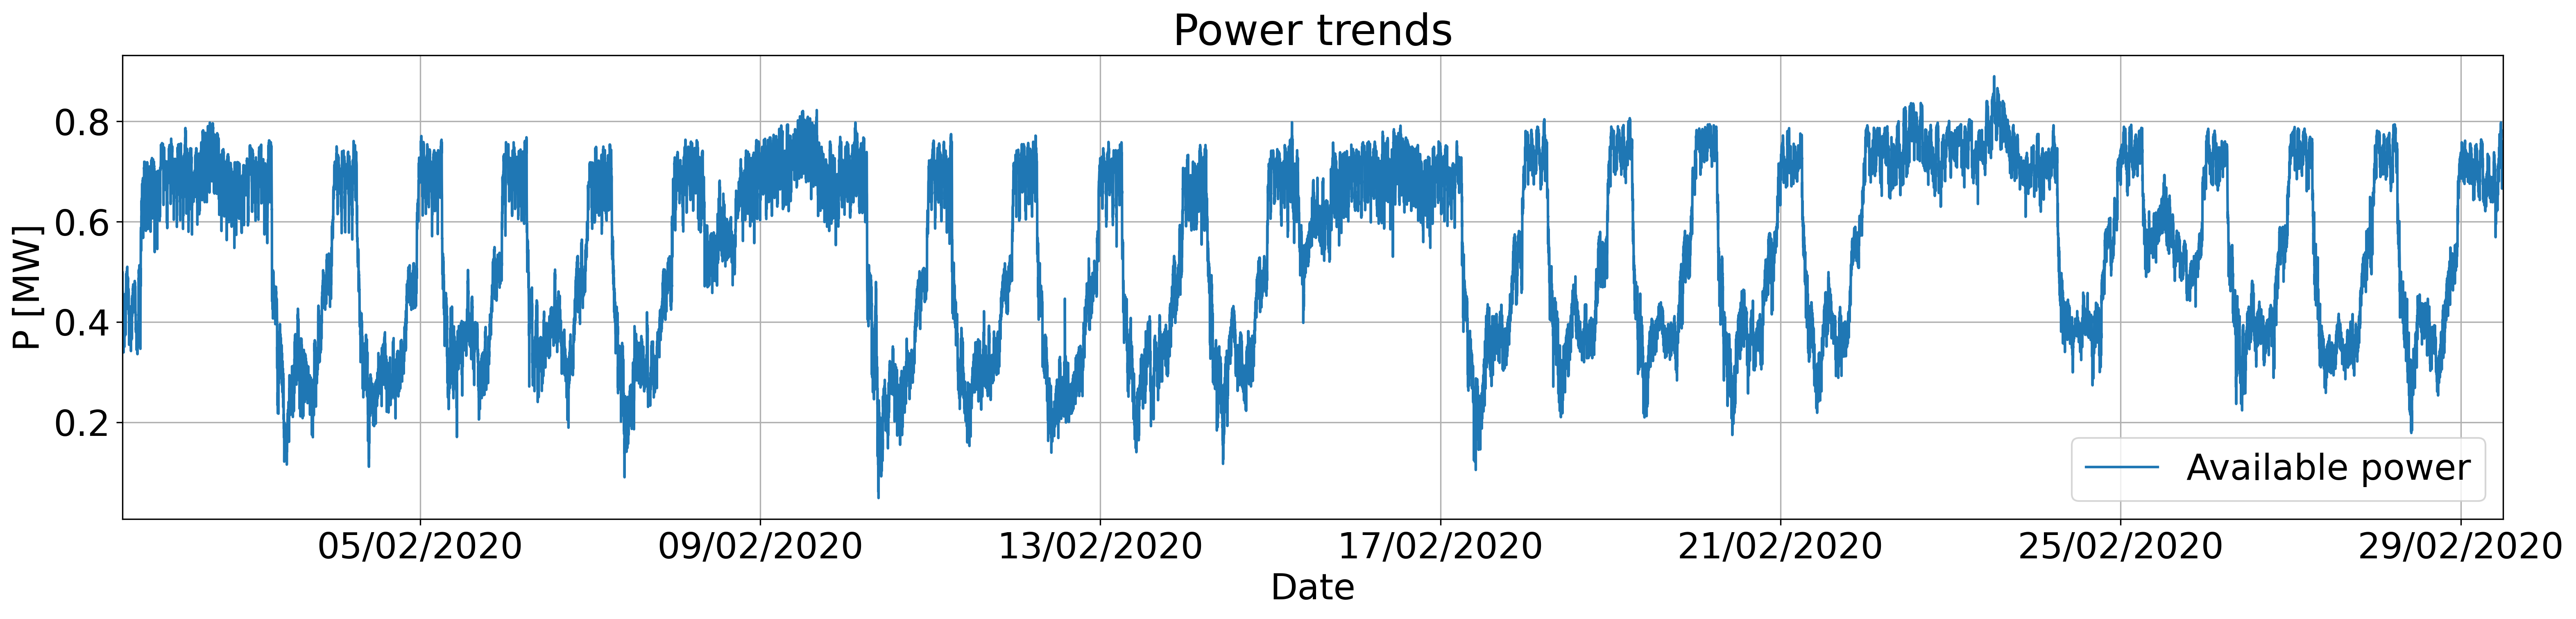
\includegraphics[width=1\linewidth]{Images/Available_power.png}}
    \caption{EDP's building power trends a) grid capacity, consumption and production b) available power.}
\end{figure}


By analyzing Figure \ref{Max_cons_prod}, it can be verified that, compared to the consumption presented by the building, the \ac{PV} panels do not have enough capacity for the building to be self-sustainable, that is, solar power is far from being enough to maintain the regular operation of the building. One can conclude that the influence of the power generated by the \ac{PV} panels on the available power of the building is quite limited. However, in order to make a correct evaluation, it is a parameter that must be taken into account. The value of the available power is a computed metric, given by:

\begin{equation}
   P_{available} = P_{grid} + P_{solar} - P_{consumption},
   \label{available}
\end{equation}

where $P_{grid}$ is the maximum power that is made available to the building, provided by the electrical grid, which in this particular case is around 1.2 MW, $P_{solar}$ is the active solar power produced by the \ac{PV} system, and $P_{consumption}$ denotes the the current power consumption of the building. In Figure \ref{available_power}, the available power profile is shown for the same time interval as Figure \ref{Max_cons_prod}. Like the previous variables, it shows an equally cyclical behavior.


Taking into account all the factors mentioned, it was then decided to choose solution 2, in which the value of the available power is calculated beforehand, and is then used as input for the predictive model. This solution was chosen because it is a simpler architecture and requires less computational capabilities, since the model produces forecasts for only one variable, and not for two. Furthermore, the flexibility offered by forecasting the two variables separately is irrelevant in the context of the problem, since for the proposed objective, it is not necessary to differentiate the consumption forecast from the production forecast. 

\section{Data}\label{chap3:sec:data}

In this section, we describe the datasets used in the development of this work, and also detail the data preprocessing applied to the datasets in order to have the necessary formatting to be used during the experiment.

\subsection{Data description}\label{chap3:subsec:data_description}

In the day to day of a building, there are many factors that influence its consumption and consequently, the available power. In Chapter \ref{chap:background}, some examples of work developed with the objective of predicting the energy consumption of a building were mentioned. In Appendix B, Table \ref{table1}, it is possible to verify that generally, two categories of data are used in this kind of applications, data that concern the behavior of the building, and climatic data that characterizes the surrounding environment of the building.

Regarding the energy behavior of the building, \ac{EDP} provided two different datasets that present information between January 25, 2020 and September 30, 2020, totalling 8 months and 5 days of data, with a granularity of 5 seconds. The first dataset includes historical data concerning the power consumption of the building, and the second dataset includes historical data regarding the solar power production generated by the \ac{PV} panels installed over the building. It is also relevant to mention that the production data provided showed some gaps, resulting from sensor reading failures. This aspect implies the need for some automatic mechanisms to complete the missing data, which are described below.

Regarding climate data, \ac{FCUL} provided two different datasets that present information between January 25, 2020 and June 15, 2020, totaling 4 months and 21 days of data, with a granularity of 1 minute. The first dataset includes meteorological data of the geographical location of the building, and the second includes data with respect to solar radiation exerted on the geographical location of the building. Neither of the two datasets had temporal flaws.

In Table \ref{table2}, there is a summary of the key points of the available data. The description of the variables for each of the datasets provided can be found in Appendix \ref{chapter:appendixE}, Table \ref{tab:available_variables}.

\begin{table}[htbp]
  \centering
  \caption{Summary of the datasets used.}
    \begin{tabular}{lr|cccc}
    \toprule
    \multicolumn{2}{c|}{\textbf{Provider}} & \multicolumn{2}{c}{\textbf{EDP}} & \multicolumn{2}{c}{\textbf{FCUL}} \\
    \midrule
    dataset &       & Consumption & Production & Meteorological & Radiation \\
    \# variables &       & 8     & 7     & 21    & 27 \\
    period &       & \multicolumn{2}{c}{8 motnhs and 5 days} & \multicolumn{2}{c}{4 motnhs and 21 days} \\
          & beginning date & \multicolumn{2}{c}{25-01-2020} & \multicolumn{2}{c}{25-01-2020} \\
          & ending date& \multicolumn{2}{c}{30-09-2020} & \multicolumn{2}{c}{15-06-2020} \\
    \# days &       & \multicolumn{2}{c}{249} & \multicolumn{2}{c}{142} \\
    \# samples &       & \multicolumn{2}{c}{4302720} & \multicolumn{2}{c}{2453760} \\
    \end{tabular}%
  \label{table2}%
\end{table}%


As can be seen through the analysis of Table \ref{table2}, the data provided do not portray the same time window nor have the same granularity. It is then necessary to proceed to some data treatment in order to obtain the data in the desired form.

\subsection{Data completion}\label{chap3:subsec:data_completion}

The data completion consists of a process in which the data made available is formatted in such a way that it meets the essential criteria to enable its introduction in the models. During the development of the thesis, this was the most time consuming process. The data treatment is an extremely demanding process, which is illustrated in the diagram of Figure \ref{datatreatment}.

\begin{figure}[h!]
    \centering
    \begin{center}
    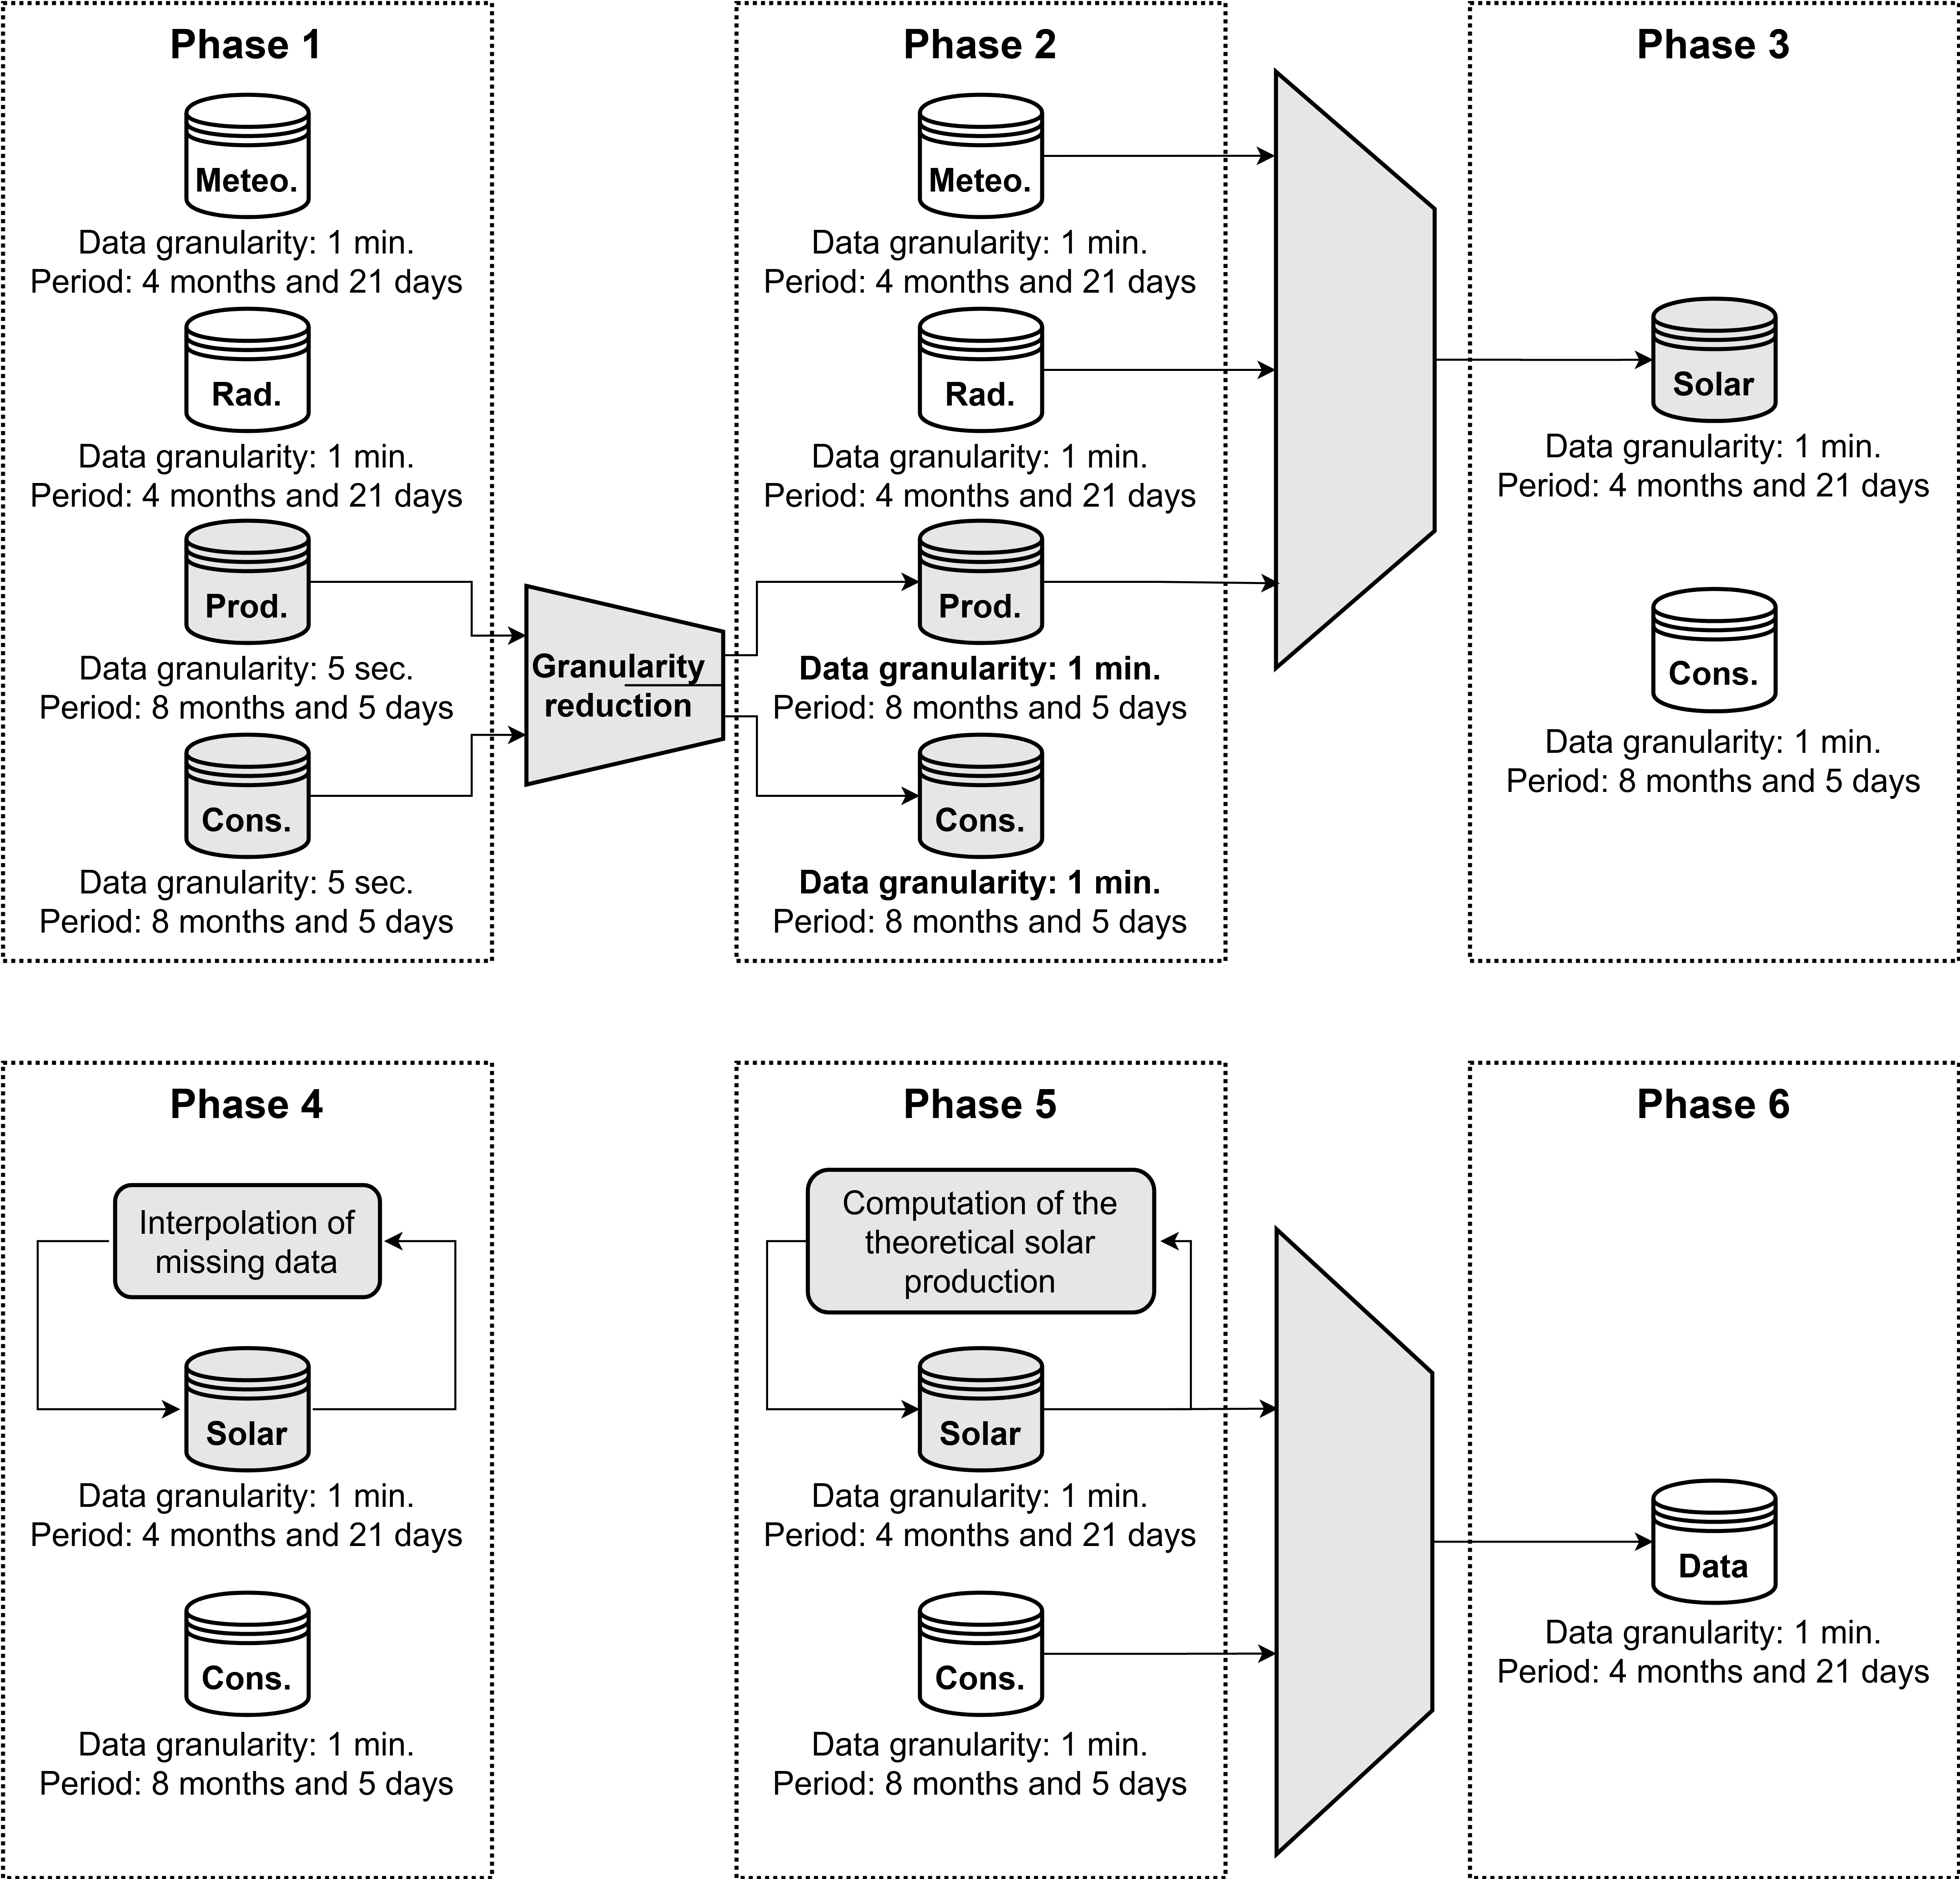
\includegraphics[width=1\textwidth]{Images/Data.png}
    \caption{Data treatment process.}
    \label{datatreatment}
    \end{center}
\end{figure}

In Phase 1, the production data (Prod.) is incomplete due to failure of the system responsible for acquiring and storing this indicator. There is also a difference both in granularity and period available, between the data provided by \ac{EDP} and the data provided by \ac{FCUL}. It is then necessary, first of all, to equal the granularity of all four datasets. In order to do that, a function was applied to reduce the granularity of the production (Prod.) and consumption (Cons.) datasets, forcing the frequency of both datasets to one minute. The function applies an arithmetic mean given by 

\begin{equation}
     A={\frac {1}{n}}\sum _{i=1}^{n}a_{i}={\frac {a_{1}+a_{2}+\cdots +a_{n}}{n}},
\label{amean}
\end{equation}

where $A$ represents the value of the final measure with frequency of 1 minute, and $n$ represents the number of nodes between that minute range that will be converted to a single value. We then reached Phase 2, where the four datasets have the same granularity. Then, the datasets corresponding to the meteorological data \textit{Meteo.}, radiation data \textit{Rad.} and production data \textit{Prod.} are concatenated. As a result of this process (Phase 3), the dataset \textit{Solar} is formed, which aggregates all the information regarding climate data and solar production data over a period of 4 months and 21 days. The reason behind this phenomenon is that all the production days for which there is no direct correspondence in the meteorological data \textit{Meteo.} and radiation data \textit{Rad.} datasets are dropped. 

As mentioned before, the data regarding the solar production \textit{Prod.} presented some temporal flaws. In order to solve the problem, two solutions were found. For time gaps of less than 30 minutes (Phase 4), a quadratic interpolation was applied. As an example, given any three points $(x_0, f(x_0))$, $(x_1, f(x_1))$ and $(x_2, f(x_2))$, the polynomial that interpolates the three points is given by

\begin{equation}
\begin{split}
     & f_2(x)=b_0+b1(x-x_0)+b_2(x-x_0)(x-x1),\\
     & where:\\
     & b_0=f(x_0),\\
     & b_1=f[x_0,x_1]=\frac{f(x_1)-f(x_0)}{x_1-x_0},\\
     & b_2=f[x_0,x_1,x_2]=\frac{\frac{f(x_2)-f(x_1)}{x_2-x_1}-\frac{f(x_1)-f(x_0)}{x_1-x_0}}{x_2-x_0}.\\
\end{split}
\label{poly}
\end{equation}


In order to exemplify the evolution of the incomplete dataset construction, in the chart of Figure \ref{int0} one can observe the solar power generated measured by the sensors on February 24, 2020. In red, is the portion of data that were measured, corresponding to the Solar dataset in Phase 3 represented in Figure \ref{datatreatment}. After the interpolation, to the original dataset are added the points represented in blue, which represent measurement failures of less than 30 minutes, resulting from the interpolation procedure explained before. At the end of Phase 4, the dataset is then composed of the data points represented in blue plus the points represented in red.



\begin{figure}[h!]
    \centering
    \begin{center}
    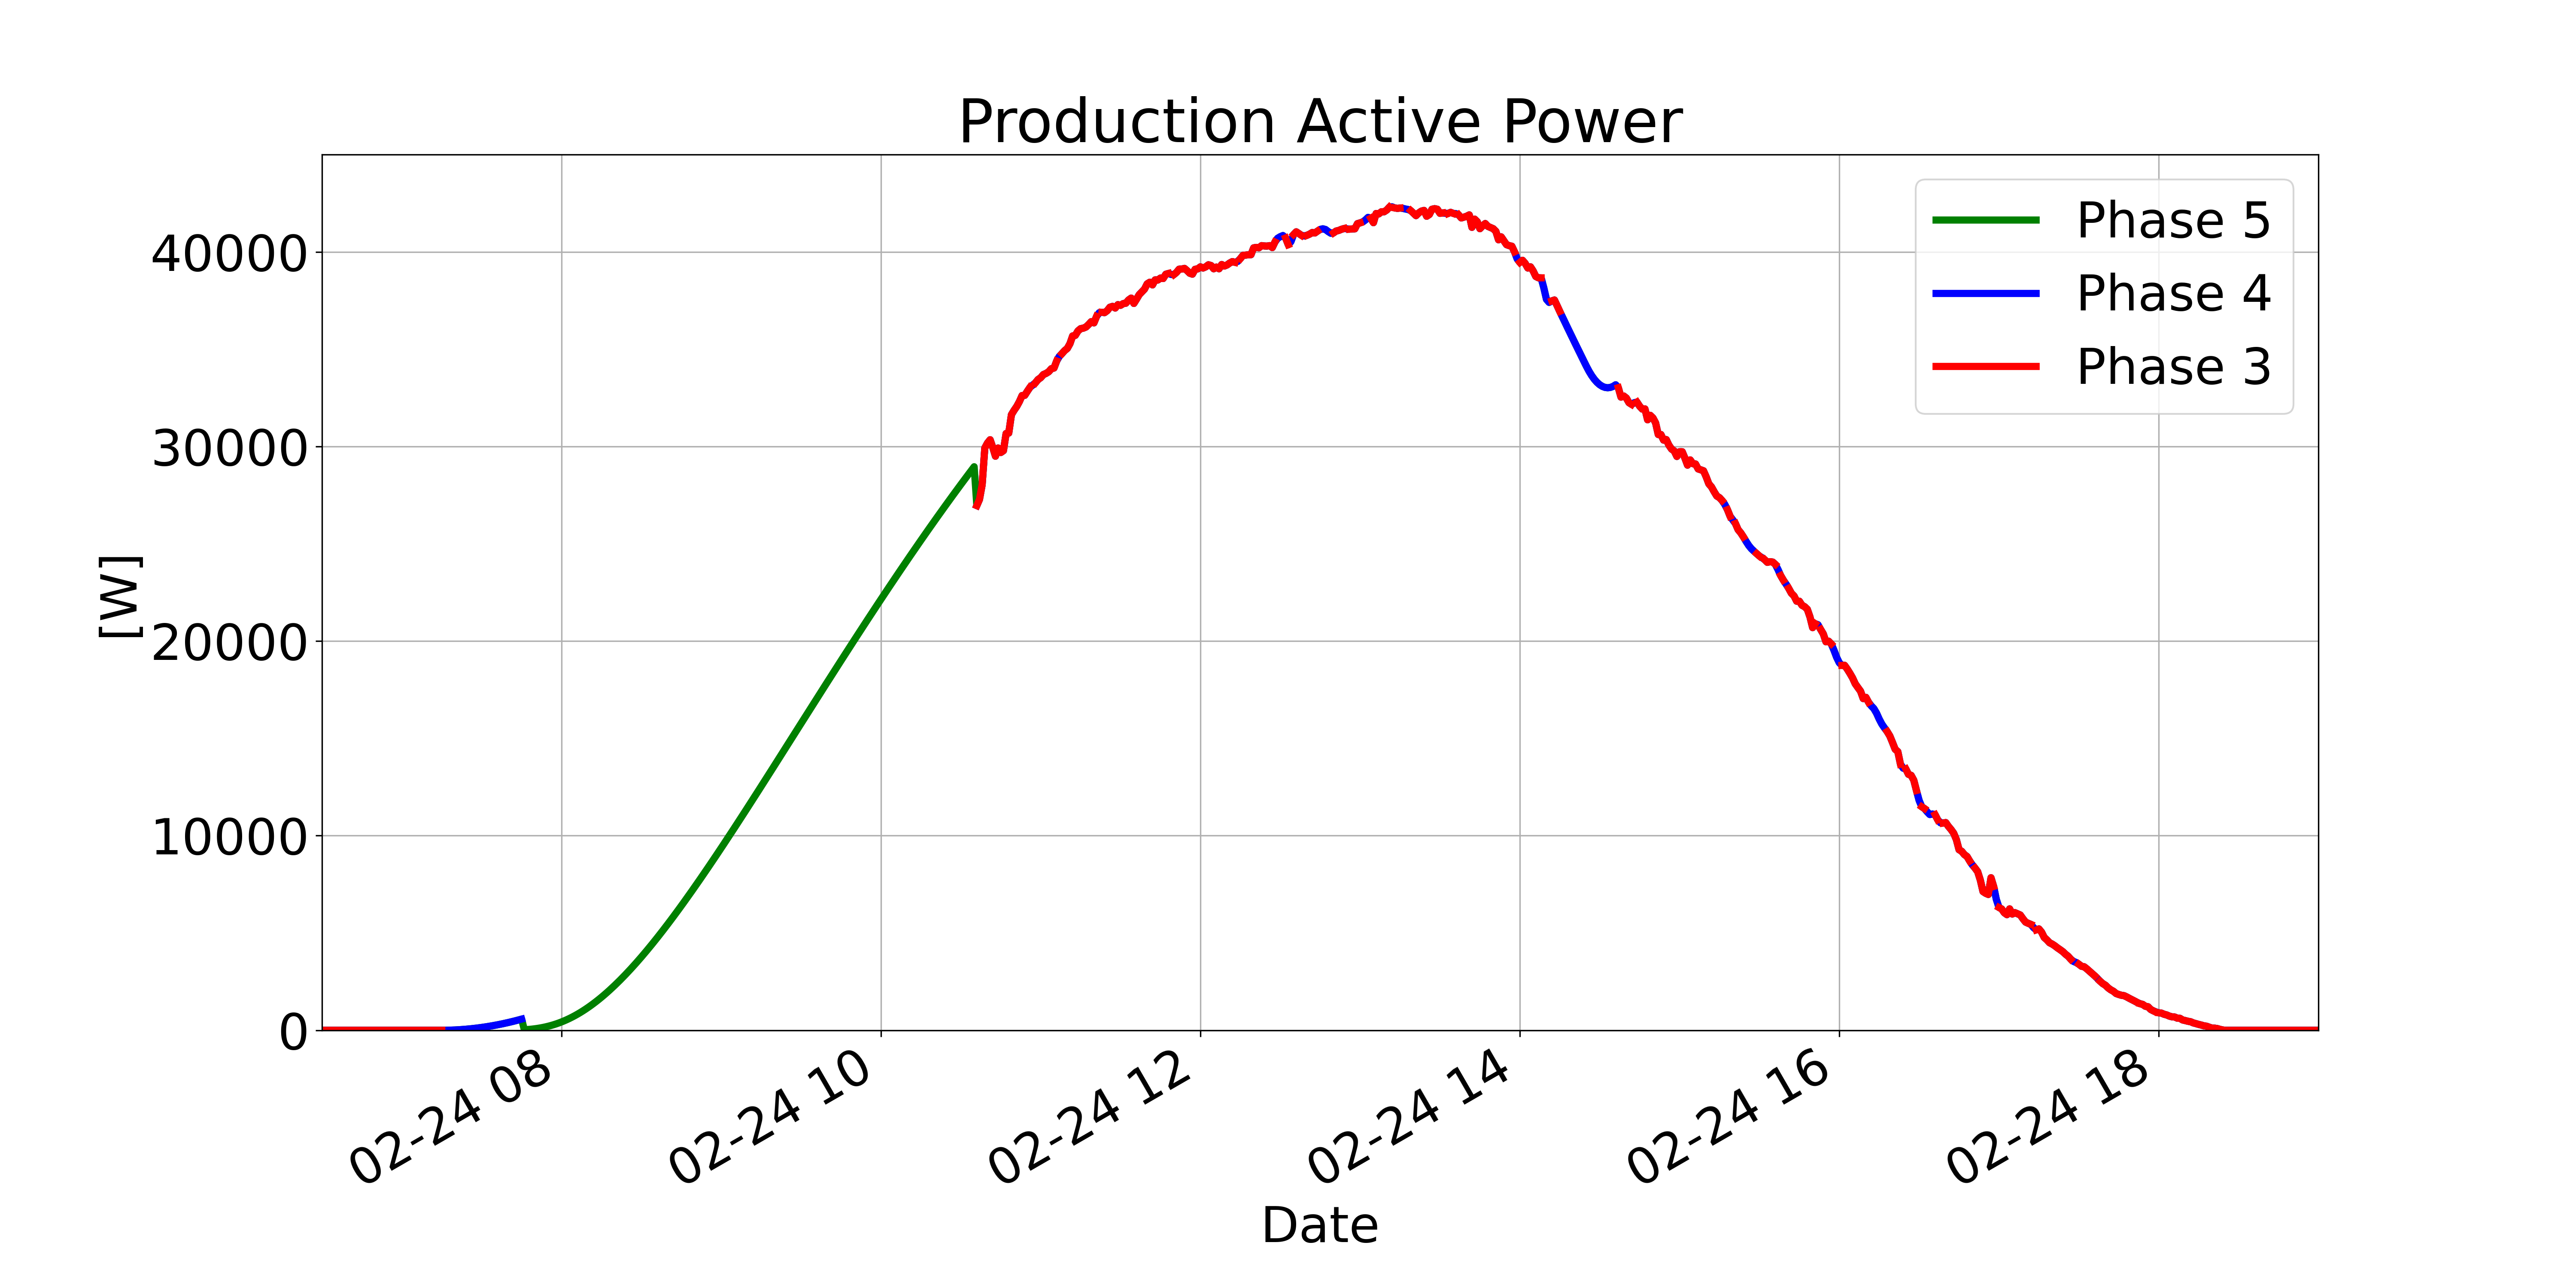
\includegraphics[width=1\textwidth]{Images/int0.png}
    \caption{Data treatment process.}
    \label{int0}
    \end{center}
\end{figure}

For time failures of over 30 minutes, the dataset was completed with theoretically computed values, since the interpolation for large temporal failures does not present the expected behavior.
Based on the equation of the sun's position in the sky throughout the year, the maximum amount of solar insolation on a surface at a particular tilt angle can be calculated as a function of latitude and day of the year\cite{solar0}. In order to determine the direct component of solar radiation in $kW/m^2$, one used


\begin{equation}
     I_D = I_0*0.7^{(AM^{0.678})},
\label{solar}
\end{equation}

where $I_0$ is the solar intensity external to the Earth's atmosphere that is approximately $1.353 kW/m^2$, $0.7$ represents the overall attenuation of the atmosphere, $AM = \frac{1}{cos\theta}$ is the airmass and $\theta$ is the zenith angle (90° minus the altitude) of the sun. This formula produces an optimal result when there are no clouds. Multiplying the resulting value by the total area of panels in the building and taking into account their positioning efficiency, a theoretical value of power generated by the \ac{PV} panels is obtained, in an ideal scenario. In Phase 5, all missing readings were replaced by the calculated theoretical value, as can be seen in Figure \ref{int0} in green. This way, the Solar dataset was completed. It is possible to verify that the point of change between the theoretical data (the green one) and the original data (the red one) is somewhat sudden, because the green signal considers an ideal scenario and the red signal represents real measurements (affected by clouds, cranes, etc.). The sum of the green, blue and red signals, result in a complete signal for the solar active power generated by the \ac{PV} panels. 


The completion process of the \textit{Prod.} dataset could have been done before joining it with the other datasets (\textit{Meteo.} and \textit{Rad.}) in the Solar dataset, but it was decided to first reduce the size of the total set from 8 months and 5 days to 4 months and 21 days (Phase 2 $\to$ 3), and only then, with the \textit{Solar} dataset already created, perform the necessary computations to complete the missing data. The two completion procedures described before are computationally expensive, so reducing the size of the dataset to be completed to half of its initial size has a major impact on the running time of the whole process. It is important to emphasize that, although the Phases 4 and 5 present in Figure \ref{datatreatment} present the process of interpolation and computation of the theoretical solar value regarding the whole Solar dataset, these procedures were applied exclusively to the features concerning production, since these were the only ones that were incomplete until then.



In Phase 6 the \textit{Solar} and \textit{Cons.} datasets were concatenated, thus reducing the dataset time interval to a final result of 4 months and 21 days.

\subsection{Data partition}\label{chap3:subsec:data_partition}

In order to study a certain algorithm, it is necessary to have access to past data to train the model and then evaluate its performance. The available data is key point when it comes to developing predictive models. Usually, in \ac{ML}, to study a certain model, the dataset should be divided into three sets as can bee seen in Figure \ref{division}. 

\begin{figure}[h!]
    \centering
    \begin{center}
    
\includegraphics[width=1\textwidth]{Images/division.png}
    \caption{Dataset division.}
    \label{division}
    \end{center}
\end{figure}

The first set is known as a training set, and consists of a dataset used to feed the model with examples in order to fit the hyperparameters, such as the weights of connections between neurons in \ac{ANNs}. As the name implies, the training set is suitable to train the model, progressively adapting the model to its intended purpose. The second set is for validation, which is responsible for simultaneously continuing to adapt the hyperparameters of the model, while providing an unbiased evaluation of the model fit. In addition to that, it can be used for regularization, as will be explored in a later section. Finally, the test set is an independent dataset of the two previous ones, which has the main objective to evaluate in an unbiased way the performance of the model in unseen data (data that was not used neither in the training process, nor in the validation process). 

One way to use the available dataset to evaluate the proposed models would be to simply apply the standard training-validation-testing division to the entire dataset available, but this strategy would be a poor way to use the small amount of data available. Typically, to evaluate machine learning models on a very limited time interval, k-fold cross-validation is used. This methodology consists, in the first place, in splitting the dataset into K folds. The higher the K value, the less biased the model is, but on the other hand, small folds (large value for K) can lead to errors due to lack of data, so one should choose the K value based on the data available for the specific application. Secondly, the model is trained in K-1 folds and validated on the remaining fold. This process is repeated until all the K folds have served as the validation set. The average performance on all validation folds shows a more robust result of the model performance evaluation than the standard train-validation-test methodology presented above. However, k-fold cross-validation can present some problems when applied to time-series problems, since one cannot choose random samples and assign them to either the validation set or the training set because it makes no sense to use future values to predict past values. There is a time dependency between observations, and it is essential to preserve this relationship during the entire process. To overcome this barrier, a nested cross-validation method was used. This validation methodology is an alternative to k-fold cross-validation that retains the temporal dependence of data. This procedure is quite complex, but according to the literature, it has the ability to "provide an almost unbiased estimate of the true error" \cite{nested}. It consists, in the first place, of splitting the data into different blocks, whose size progressively increases, implementing an expanding window approach. Then, each of these blocks must be split into train, validation and test data, where the validation data, as in the standard methodology, is temporally subsequent to the training data. In this procedure there are two loops, the inner loop and the outer loop. The inner loop is done with the purpose of tuning the hyperparameters for each of the blocks. After defining the optimal hyperparameters for each block, the model is retrained with these hyperparameters and tested in the test block. The outer loop consists of repeating this process for the 4 available blocks. 

After applying this procedure to the different blocks available, an average of the validation errors and an average of test errors presented in the different blocks is then calculated, thus reaching a total validation and testing error value. This methodology brings great advantages when the access to data is limited. It allows the user to make a much more robust evaluation of the performance of each model considering multiple scenarios.

In Figure \ref{partition}, the reader may find four different sub-datasets, resulting from a division of the main datastet, defined in phase 6, of the section \ref{chap3:subsec:data_completion}. The idea behind this division is to use 4 subsequent blocks for nested cross-validation, in order to conduct hyperparameter tuning of the different architectures proposed. In a second stage, after tuning the hyperprameters in each of the four blocks, one moves on to the test phase, in which the model to be tested, already with the hyperparameters defined, is retrained and tested in the Test set.

\begin{figure}[h!]
    \centering
    \begin{center}
    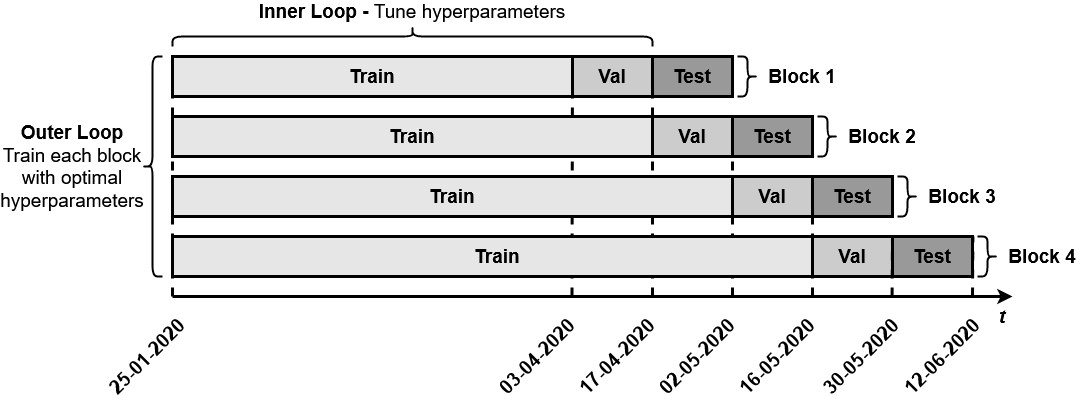
\includegraphics[width=1\textwidth]{Images/hyptun_.png}
    \caption{Data partition diagram.}
    \label{partition}
    \end{center}
\end{figure}

The performance evaluation of the models is then given by the average of the performance in each of these blocks i.e., the test error of the models is given by

\begin{equation}
     Model\ test\ error =\frac {1}{k}\ \sum_{i=1}^k Error_{di},
\label{err_av}
\end{equation}

where $Model\ test\ error$ represents the final model error for all the test sets, $Error_{di}$ represents the error that the model presented while performing in dataset $i$, and $k$ represents the number of datasets used.
In this specific case, the test error for each model is given by

\begin{equation}
     Model\ test\ error =\frac {1}{4}\ (Error_{testb1} + Error_{testb2} + Error_{testb3} + Error_{testb4}).
\label{err_av}
\end{equation}

The great advantage of using this method is the attenuation of the influence of random errors. In other words, by performing an average of the errors in the four different sets, the robustness of the selection process is increased since different scenarios are considered.


\subsection{Data shifting}\label{chap3:subsec:data_shifting}

While designing a predictive model, the training process is critical so that the model can learn from the data supplied to it. In a time series problem, it would not make sense for the input data to be of the same instant as the output data. When one wants to determine a future value based on current conditions, one needs to train the model to use the input data of the current instant to predict the output data of a future instant. It is then necessary to apply a shift to the output data so that training the model builds a predictive logic, also known as converting the time series into a supervised learning series. If the shift was not applied, one would be training the model to, based on the current instant data, determine the output data of the current instant, and that is not what is intended. As it is already known, one of the main objectives of this thesis is to forecast the available power of the building in 5, 10 and 15 minutes. To do that, depending on the model selected for that purpose, it might be necessary to develop 3 different supervised learning series. In Figure \ref{shifting}, the reader can find a graphical representation of the performed procedure.


\begin{figure}[h!]
    \centering
    \begin{center}
    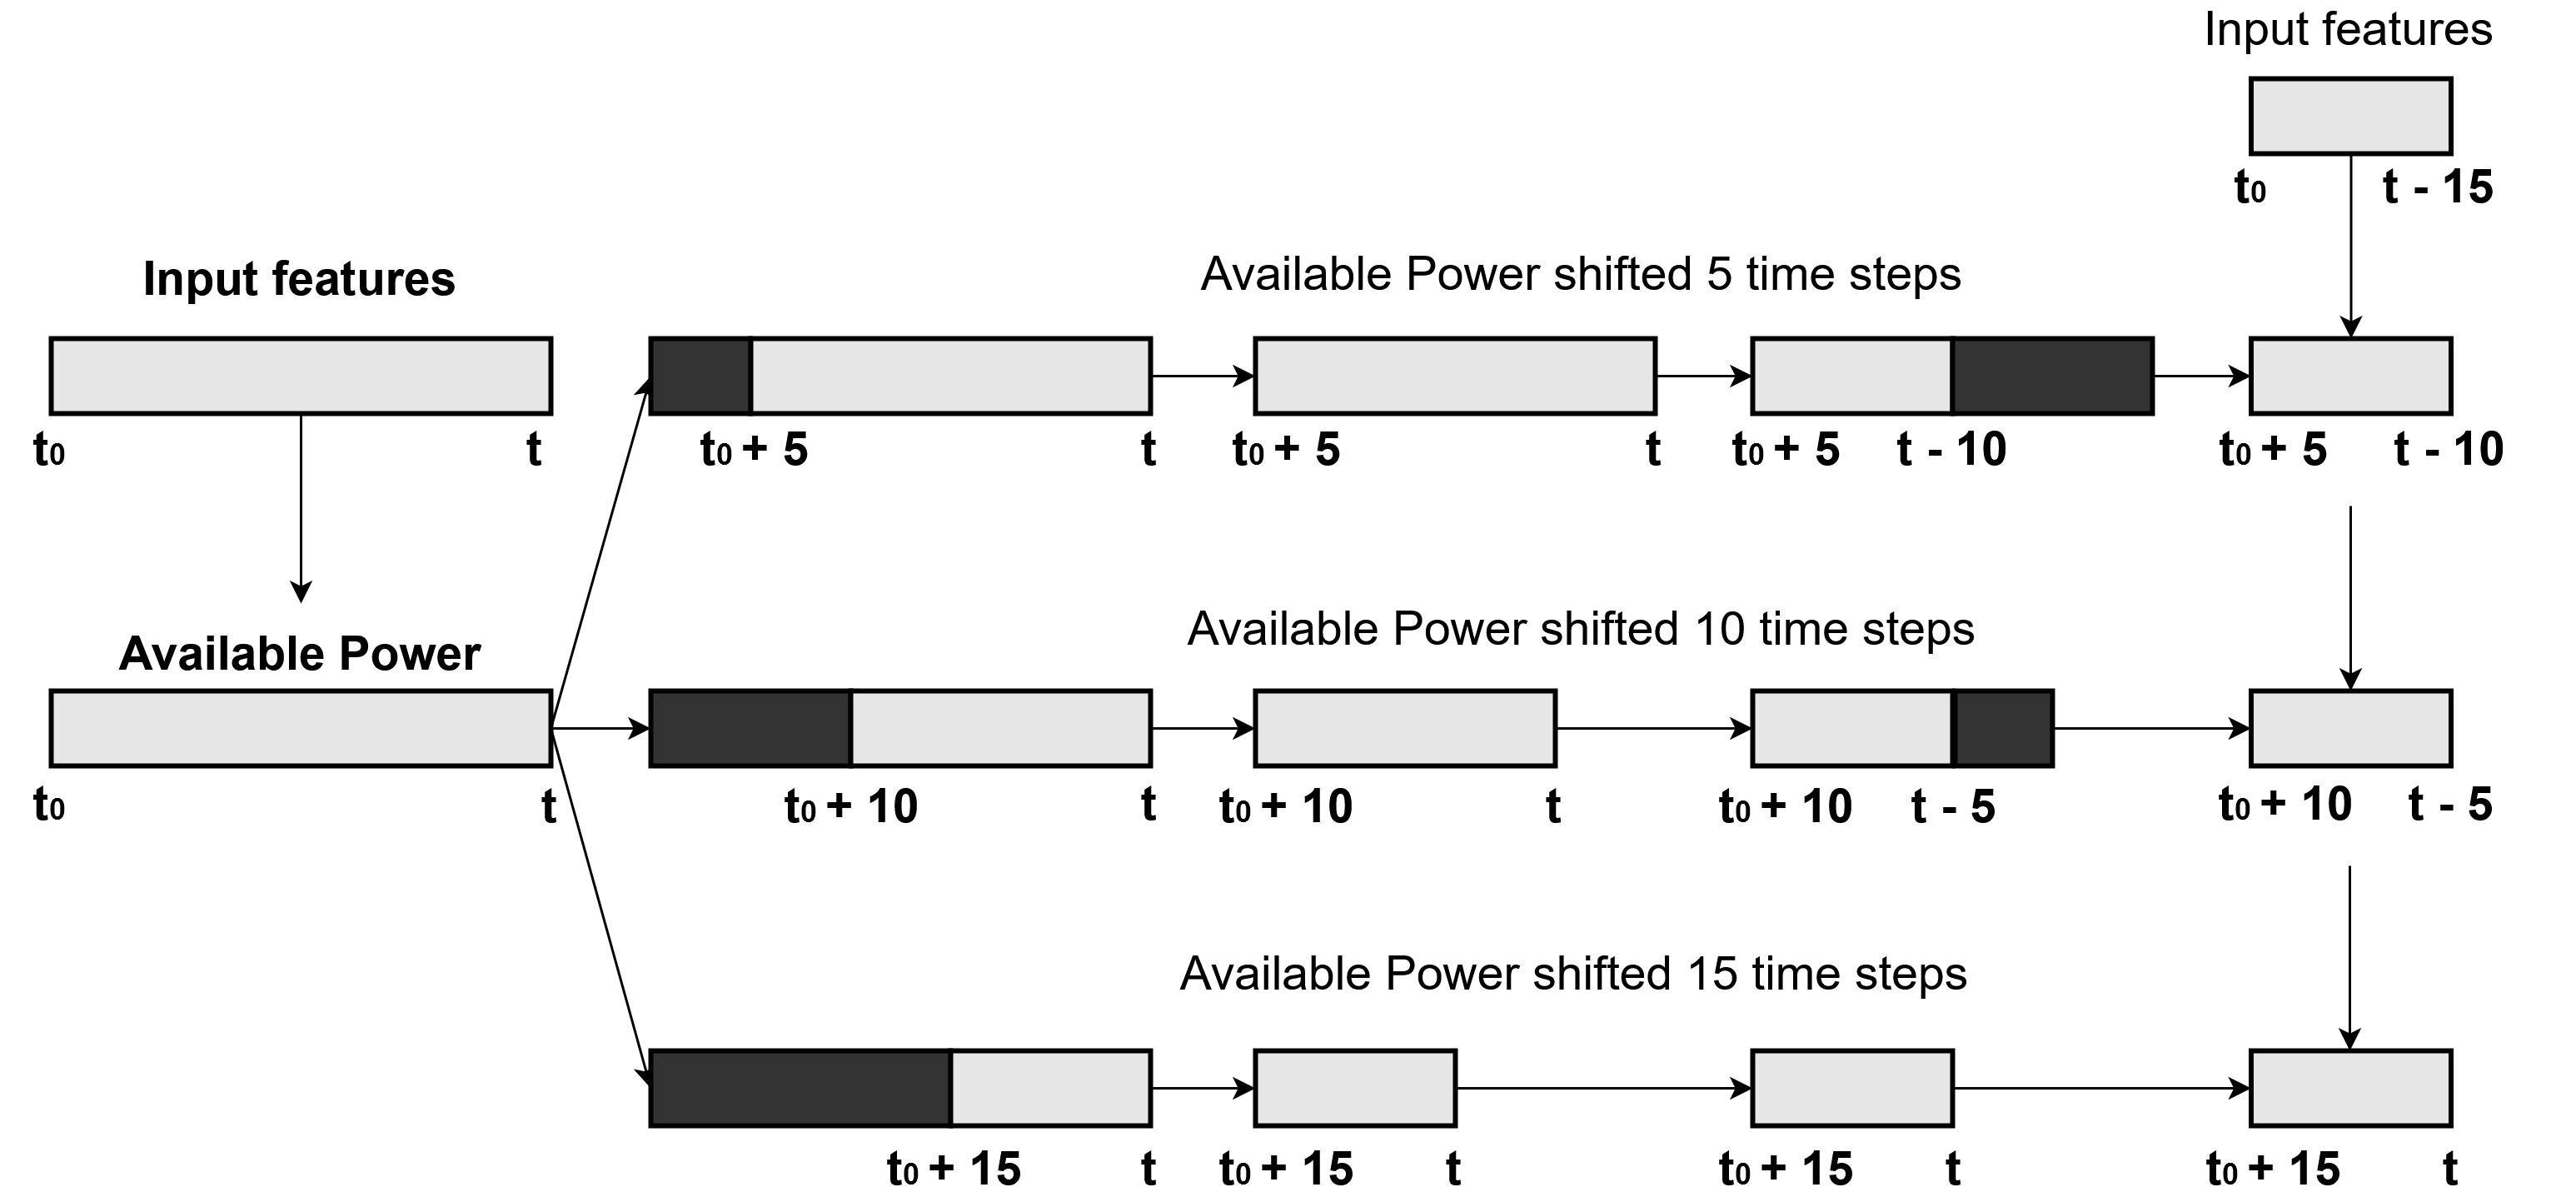
\includegraphics[width=1\textwidth]{Images/Data Shift.png}
    \caption{Data shifting procedure.}
    \label{shifting}
    \end{center}
\end{figure}

In a first instance, one has the data set that corresponds to the features identified as the input features of the model. For the initial scenario, the features of a given instant $t_i$, have a direct match with a value of Available Power of the output variables for the same instant $t_i$.  Then the transformation process begins, where the output variables will be shifted 5, 10 and 15 time-steps. The data vector of Available Power is copied originating three identical vectors. In the first step, the first 5, 10 and 15 measurements of each Available Power vector are removed, originating the output vectors with the ranges $[t_0 + 5, t]$, $[t_0 + 10, t]$, $[t_0 + 15, t]$ respectively. At this time, each set of input features already presents a match of Available Power in 5, 10 and 15 minutes, but the output vectors present different dimensions as one would expect. In order to have output vectors with the same dimension, the size of the three vectors is limited to the size of the smallest, as well as the set of input features. In the last step there is then a set of input features with values in the range $[t_0, t-15]$ and the ranges $[t\_0 + 5, t-10]$, $[t_0 + 10, t-5]$ and $[t\_0 + 15, t]$ for the Available Power to 5, 10 and 15 minutes, all four vectors with the same dimension. 

It should be noted that, depending on the chosen model, it may or may not be necessary to use the three series, this will depend exclusively on the architecture of the model used. In any case, it was thought relevant to have the three series, one in which the input features for instant t link to the output feature for $t+5$, the second in which the input features for instant t link to the output feature for $t+10$, and finally, a third series in which the input features for instant t link to the output feature for $t+15$. Another point to mention is the reduction in the dataset dimension. There is a loss of 15 time-steps of data in this whole process. Since the total dataset contains a total of 201542 time-steps, the elimination of these 15 time-steps corresponds to a loss of only 0.0074$\%$ of the information.

\subsection{Feature selection}\label{chap3:subsec:feature_selection}

Although a total of 63 different features have been made available for the development of this work (Appendix \ref{chapter:appendixE}, Table \ref{tab:available_variables}), it is necessary to select which features to use in the development of a \ac{ML} model. Besides the 63 features provided by \ac{EDP} and \ac{FCUL}, 7 other features were also selected, which are listed in Appendix \ref{chapter:appendixE}, Table \ref{tab:computed_variables}. These new features concern calendar metrics such as $hour$, $day\_of\_week$, $day\_of\_month$, $month$ and $holiday$ (a binary indicator that states whether the day in question is a national holiday or not), and also concern calculated metrics such as $AvailablePower$, whose calculation is detailed in section \ref{chap3:sec:variable_to_predict}, and the $TheorethicalValue$, which concerns the theoretical value of the power generated by the \ac{PV} panels, detailed in the section \ref{chap3:subsec:data_completion}. 

A high number of features implies a high complexity of the system architecture. Even though all these features contribute in some way to enrich the past information available, it is important to limit the number of features used. It is then necessary to perform a pre-selection of which features are ideal for the system to produce the best possible results. 

It is certain that for a good model performance, the amount of available data is an extremely relevant factor. A model that has access to more information, in general, will present a better performance than a model that has access to less information. However, it must be ensured that the data provided to the model is relevant in the context of the problem, and that it actually helps to improve its performance. So far, a set of 70 features has been accessed, but the individual contribution of each feature in the context of the problem is not the same. Using the 70 features would produce a heavy and inefficient model, as there may be small groups of features whose contribution to the model is the same. We are then faced with a problem of dimensionality reduction. From the 70 features, it is necessary to extract those that are relevant in the context of the problem, and that actually contribute to a more capable model.

The concept of \ac{PCA}, \cite{pca} is then introduced. \ac{PCA} is a statistical procedure whose goal is to reduce the dimensionality of large datasets, replacing a high number of features by fewer features that still contain the relevant information from the original dataset. The dimensionality reduction can often incur in an increase of the error produced by the model, but the trick relies in giving up some minor accuracy for simplicity.


The \ac{PCA} is characterized by identifying the dimensions over which data are most dispersed. This way, the dimensions that best differentiate the data set under analysis are identified, that is, its main components. Since the \ac{PCA} is sensitive to the scale of the original data, the first step is to normalize the data. To do this, on the original data, the following formula was applied to every feature individually

\begin{equation}
   Z_i = \frac{x_i-\overline{x_i}}{\sigma_i},
   \label{PCA1}
\end{equation}

where $Z_i$ represents the normalized variable, $x_i$ the original variable, $\overline{x_i}$ the mean, and $\sigma_i$ the standard deviation. From the standardized variables, the correlation matrix $\rho$ is then calculated, where each position is given by


\begin{equation}
   Q_{ij} = \frac{1}{n-1}\sum_{i=1}^nZ_{i,n}Z_{j,n}.
   \label{PCA2}
\end{equation}

After obtaining the complete correlation matrix, $\rho$, one should then extract the eigenvectors and eigenvalues, two important factors that contribute for finding the directions of maximum variance and the the value of that variance, respectively. In fact, the eigenvalues are the are  the  variance  of  principal  components. In order to extract eigenvectors and eigenvalues, one applied \ac{SVD}, that states that a matrix A with $n$ rows and $p$ can be decomposed in 

\begin{equation}
   A_{n,p} = U_{n,n} S_{n,p} V^T{p,p},
   \label{PCA3}
\end{equation}

where the columns of matrix $U$ are the left singular vectors, the $S$ is a diagonal matrix that has the same dimensions as A, and contains the singular values along the diagonal, and $V$ is the transposed orthogonal matrix and its rows are the right singular vectors. By multiplying $A^TA$, one gets exactly the matrix $\rho$, so 

\begin{equation}
   \rho = A^TA = VS^2V^T,
   \label{PCA4}
\end{equation}

thus V can be determined. Eigenvectors of matrix A are then found, and the $k$ eigenvectors that correspond to the $k$ directions of maximum variance are selected. The value of $k$ is is chosen based on the cumulative explained variance where the variance of several components is added together and divided by the total variance. This procedure is progressive, where the number of components used increases. With the increase of the number of components, there is also an increase the cumulative explained variance until it stops increasing. The point where this parameter stops increasing and stabilizes is the ideal point, where one can find the minimum value of $k$ for which the cumulative explained variance is maximum. Later, a matrix containing the selected eigenvalues is constructed which is multiplied by the original matrix A. This results in a $n,k$ matrix, the matrix resulting from the entire dimensional reduction process with the $k$ features relevant in the context of the problem.



%\subsubsection{Correlation Matrix}

%The criteria used for this selection of of meteorological and radiation data, included selecting unique features that were directly associated with the temperature or solar radiation of the surrounding environment, since, as was verified in section \ref{chap3:sec:building}, the energy consumption of the building is directly linked to the outside temperature and weather conditions. Metrics related to atmospheric pressure and humidity were discarded. Regarding the building, the metrics that refer to the power produced and the power consumed in were selected, but only the final metrics, that is, the three-phase currents and voltages were eliminated since it is from them that the value of power consumed and produced are obtained. As these two variables are also measured, the use of currents and voltages is then discarded. All 7 metrics that relate to the schedule and calculations performed, were also considered. 

%It was then necessary to evaluate these 16 pre-selected features. Therefore, the correlation matrix between each of the 16 features was computed. 

From the 70, a set of 13 features was considered useful in predicting the available power in the building. In Figure \ref{corr}, one can then observe the correlation matrix, where the correlations between all the 13 selected features are represented. The value of the correlation is present in the [-1, 1] range, where -1 means that the features present a perfect negative correlation, 0 means that there is no correlation between them, and 1 means that there is perfect positive correlation between the two features. 


\begin{figure}[h!]
    \centering
    \begin{center}
    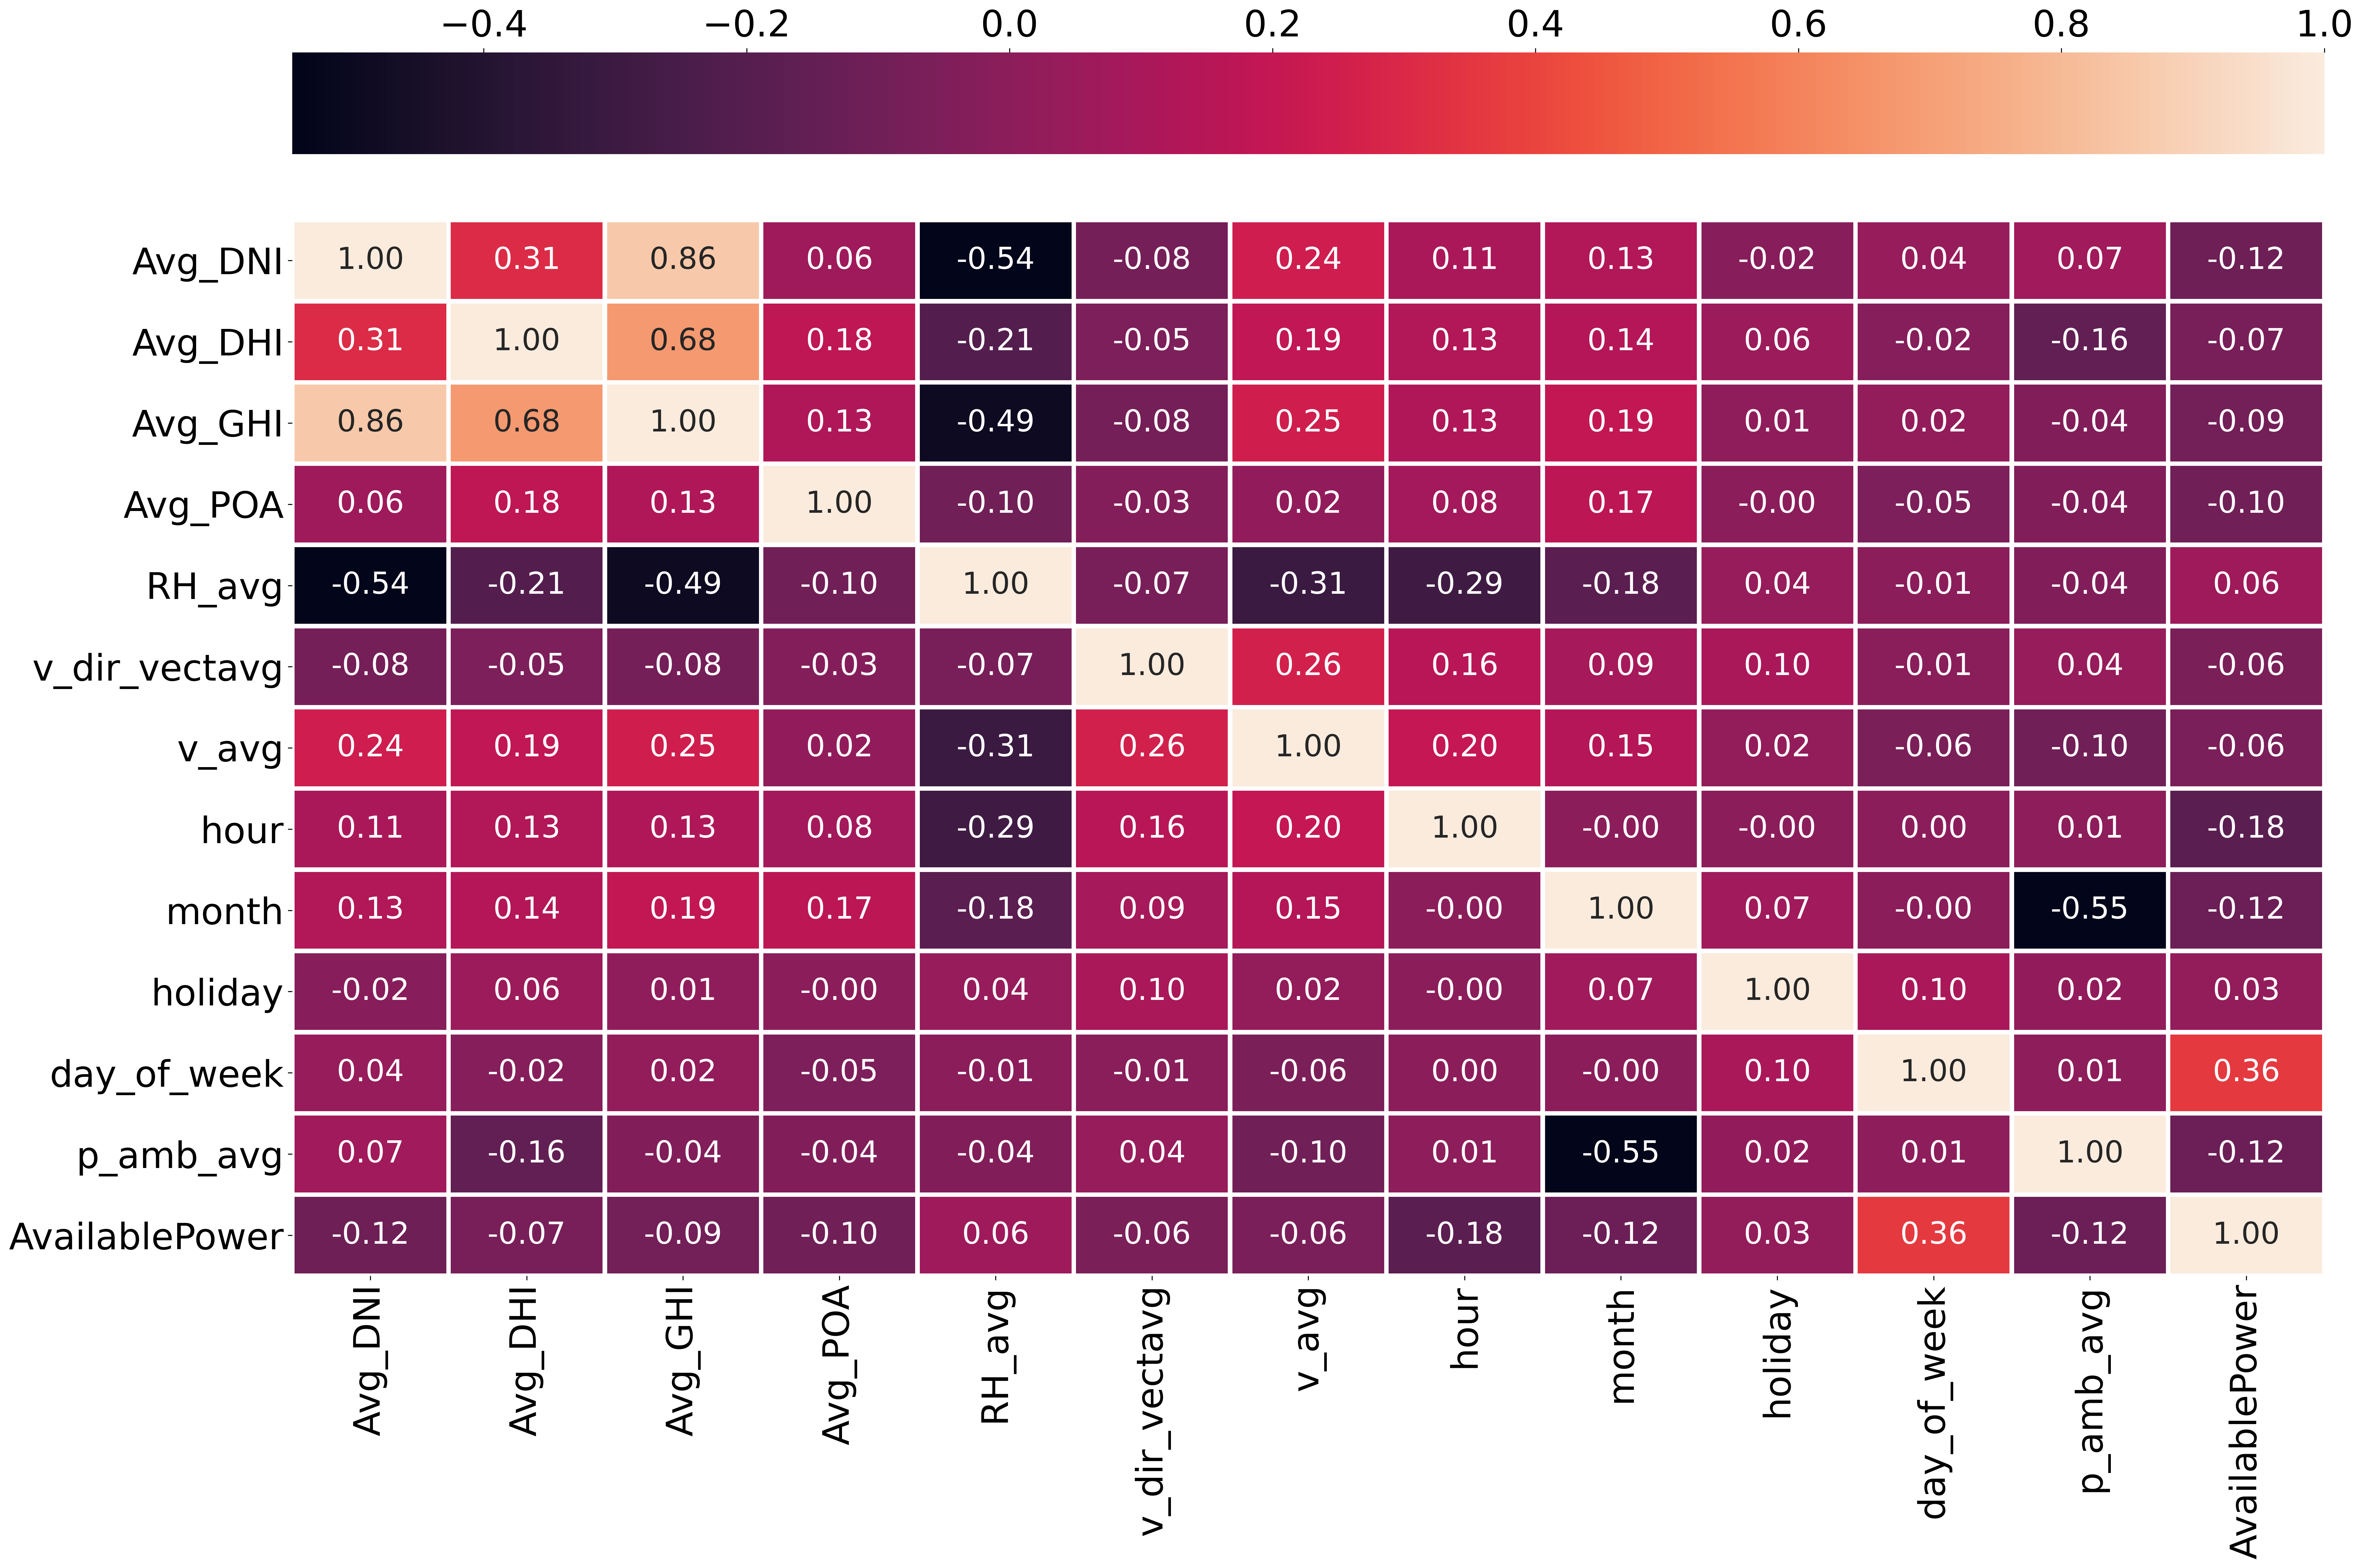
\includegraphics[width=1\textwidth]{Images/corr1.PNG}
    \caption{Feature correlation matrix.}
    \label{corr}
    \end{center}
\end{figure}


The aim of computing this matrix is to identify features that present a perfect or almost perfect correlation between them, both positively and negatively. A perfect correlation between two features means that one can be deduced from the other, that is, the relevance of the two features for the construction of the forecasting system is the same, so one of the features can be eliminated. Using features that present a perfect correlation, one can incur in multicollinearity \cite{multicollinearity}. As can be seen in the matrix present in Figure \ref{corr}, none of the features selected by \ac{PCA} presents a perfect correlation with any other. Thus, there is a minimum set of features that offers a good representation of the available data. Although all these features represent the most significant set of variables, it is not guaranteed that using all 13 features is the combination that will produce the best results, but rather that it is the set of features that presents the most distinct information. It was then vital to understand which of the features selected would produce the best results. After a trial and error process, it was verified that within the 13 features previously defined, there was a set of 8 features that would produce optimal results, being them AVG\_GHI, RH\_avg, p\_amb\_avg, hour, month, holiday, day\_of\_week and AvailablePower. 
In summary, we started with a set of 70 features where the process of \ac{PCA} was applied reducing the set to 13. Then, through a trial process where several features were combined, a final set of 8 features was obtained, which will be used as input for the proposed models.



%After evaluating the projected correlation matrix, it was decided to start to eliminate the features that present an almost perfect correlation, both negative and positive. Starting with positive correlation, S represents the complex power consumed and P the real power consumed, which means that the two values only differ in the imaginary component. Since S does not have an imaginary component, S and P have the same value. The feature S was then discarded. The Theoretical Value and ActPwr also present a perfect correlation. This happens because, as explained in section \ref{chap3:subsec:data_completion}, the readings of the power generated by \ac{PV} panels (ActPwr) showed a lot of flaws. For a time failure longer than 30 minutes, the ActPwr value (which was null) was replaced by the calculated theoretical value of power generated by \ac{PV} panels. The large correlation is then justified by the fact that there were quite a few time flaws, i.e., most of the ActPwr values are similar to the Theoretical Value. The feature Theoretical Value was also discarded. 



%Also, although Theoretical Value and Avg\_GHI present a very high correlation with ActPwr (which is predictable given that the measured ActPwr these two variables were added, as explained in section \ref{chap4:vtp}), we chose to keep these two variables as input features since the correlation is not exactly perfect and can be decisive in certain cases in building a good predictive model. Therefore, the variables chosen for the input of all tested models are: Std\_DHI, Avg\_DHI, Avg\_GHI, Avg\_DNI, Avg\_POA, T\_amb\_avg, Theoretical\ Value, ActPwr, P, hour, day\_of\_month, day\_of\_week, month and holiday. In addition, the variable Available Power given in W has been added as an input feature, resulting in a total of 15 input features and 3 output (Available Power in 5, 10 and 15 minutes).

\section{Proposed model}\label{chap3:sec:proposed_model}

In Chapter \ref{chap:background}, some of the most common models were studied with regard to forecasting power consumption in various types of buildings. As has also been mentioned, data-driven models have been widely used in this type of applications. In this thesis, it was also decided to study a solution composed by one or more data-driven models, since historically they present a better performance and an excellent relation between the need of computational resources used, and the obtained performance.

This problem presents some characteristics that are determinant in the process of choosing the models to be tested. First of all, the data made available for this study, represents a significantly short time period, which means that the use of models as statistical regressions are not ideal to solve this problem. On the other hand, the challenge presented by \ac{EDP} implies a 5, 10 and 15 minute data forecast. This factor implies the use of a fast model that is able to produce different forecasts in a short period of time. This is a problem for \ac{SVM}s/\ac{SVR}s because, as mentioned in \cite{svm3}, \cite{svm2} and \cite{svm5} while producing results with good precision an accuracy, they are slow models for large-scale problems. 

Another model presented in Chapter \ref{chap:background}, were the \ac{DT}s. Although they are simple to apply models, \ac{DT}s have the limitation of not allowing a future value to be computed, but rather a range of values in which the variable to be predicted can be found. Since for this problem the main objective is to obtain specific values of available power, this category of models was not considered in this research.

Although all the mentioned models can produce acceptable results for the proposed work, it was decided to apply different types of artificial neural networks, both architectures with only one \ac{ANN} layer, and architectures with multiple layers implemented simultaneously. The idea is then to test various topologies of \ac{ANN}s, and elaborate a comparative study between the proposed solutions, comparing their performance in different scenarios and conditions.

\subsection{Artificial Neural Networks}\label{chap3:subsec:artificial_neural_networks}

Neural networks have proven extremely efficient in identifying and learning temporal data patterns, many of them quite complex. In chapter \ref{chap:background}, two large families of neural networks were presented, \ac{FFNN}s and \ac{RNN}s. From the different existing architectures within these two categories, two types of layers were selected, \ac{GRU} and \ac{LSTM}, both classified as \ac{RNN}s' layers. In addition, \ac{1D CNN} layers were also tested, which fall under the umbrella of \ac{CNN}. These three different types of layers were tested in multiple arrangements and combined with each other to form multiple neural network architectures.

\subsubsection{Long short-term memory (LSTM)}\label{chap3:subsubsec:lstm}

The first type of configuration considered is the \ac{LSTM}, architecture that fits within the group of \ac{RNN}s, proposed et el. \cite{lstm0} by Hochreiter and Schmidhuber in 1997. \ac{LSTM}s were invented to fight the vanishing gradient problem that is often identified during the training process of common \ac{ANN}s with gradient-based learning methods and back propagation. In these cases, each of the \ac{ANN}'s weights receives an update proportional to the partial derivative of the error function from the current weight in each iteration of training. The problem is that, in some cases, the gradient becomes smaller and smaller with each iteration, preventing the weight from changing its value. This problem leads to a poor performance of the \ac{ANN}, and can even prevent it from continuing the training process. To avoid this situation, the \ac{LSTM} units are composed of a cell state, an input gate, an output gate and a forget gate, as can be seen in Figure \ref{lstm}.

\begin{figure}[h!]
    \centering
    \begin{center}
    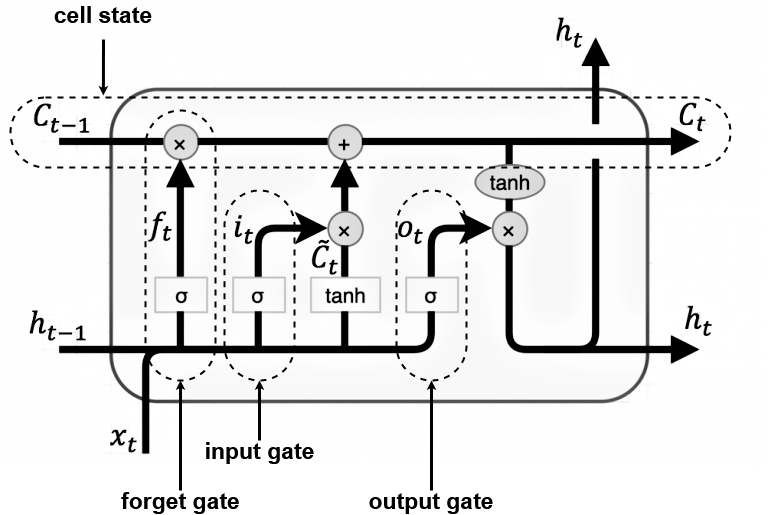
\includegraphics[width=0.6\textwidth]{Images/LSTM_cell_detailed.png}
    \caption{LSTM unit.}
    \label{lstm}
    \end{center}
\end{figure}

The responsibility of the cell state is to trace the dependencies between the elements in the input sequence. The forget gate has the purpose of forgetting information that is no longer useful to the state of the cell. This gate has two inputs, $x_t$ (input at the specific time) and $h_{t-1}$ (output from previous cell) which are multiplied by weight matrices, followed by the addition of the bias. The result of this process is passed through a sigmoid $\sigma$ activation function, which provides a binary output. If for a given cell state the output is 0, the information is forgotten, if the output is 1, the information is retained for future use.

The input gate is responsible for adding useful information to the cell state. First, the information is regulated using the sigmoide function that filters the values to be remembered in a similar way to the forget gate, also having as inputs $h_{t-1}$ and $x_t$. In parallel, a vector is created using the $tanh$ function that has as output a value in the range $ [-1, +1]$, which contains all possible values of $h_{t-1}$ and $x_t$. The values of the vector and the regulated values are then multiplied. 

The output gate's task is to extract useful information from the current cell state to be presented as an output. First, a vector is generated by applying the function tanh to the cell. In parallel, the information from the $h_{t-1}$ and $x_t$ inputs is regulated using the sigmoid function that filters the values to be remembered. The values of the vector and the regulated values are then multiplied to be sent as an output and input to the next cell.

 


The equations that describe the operation of a \ac{LSTM} unit are given by 

\begin{equation}
    \begin{cases} 
        
        f_t=\sigma(W_f.[h_{t-1},x_t] + b_f)\\
        i_t=\sigma(W_i.[h_{t-1},x_t] + b_i)\\
        \widetilde{C}_t = tanh(W_c.[h_{t-1},x_t] + b_C)\\
        C_t=f_t*C_{t-1}+i_t* \widetilde{C}_t\\
        o_t=\sigma(W_o.[h_{t-1},x_t] + b_o)\\
        h_t=ot*tanh(C_t)
        
         
    \end{cases} ,
\end{equation}

where $f_t$ represents the forget, $i_t$ the input gate, $\widetilde{C}_t$ the cell input activation vector, ${C}_t$ the cell state vector, $o_t$ the output gate, $h_t$ the hidden state vector or output vector of the \ac{LSTM} unit. This type of units has then the ability to choose new information that is relevant and delete the past information that is not relevant, maintaining a good functioning, particularly in time series data since there can be lags of undefined length between important events in a time series dataset.

\subsubsection{Gated recurrent unit (GRU)}\label{chap3:subsubsec:gru}

The \ac{GRU} unit is quite similar to \ac{LSTM} with the particular difference that it has no output gate. Introduced in 2014 by Kyunghyun Cho et el. \cite{gru0}, \ac{GRU}s are also part of the \ac{RNN} family. Although they have a similar architecture to \ac{LSTM}s, \ac{GRU}s are simpler models which led to the conclusion that for some cases, where there are smaller datasets and with a lower frequency of repetition, \ac{GRU} architectures perform better than \ac{LSTM} architectures \cite{gru1}, \cite{gru2}.

Compared to \ac{LSTM}s, \ac{GRU}s have no cell state and use the hidden state to transfer information. This architecture has only two gates, a reset gate and an update date, as can be seen in the diagram in Figure \ref{gru}.


\begin{figure}[h!]
    \centering
    \begin{center}
    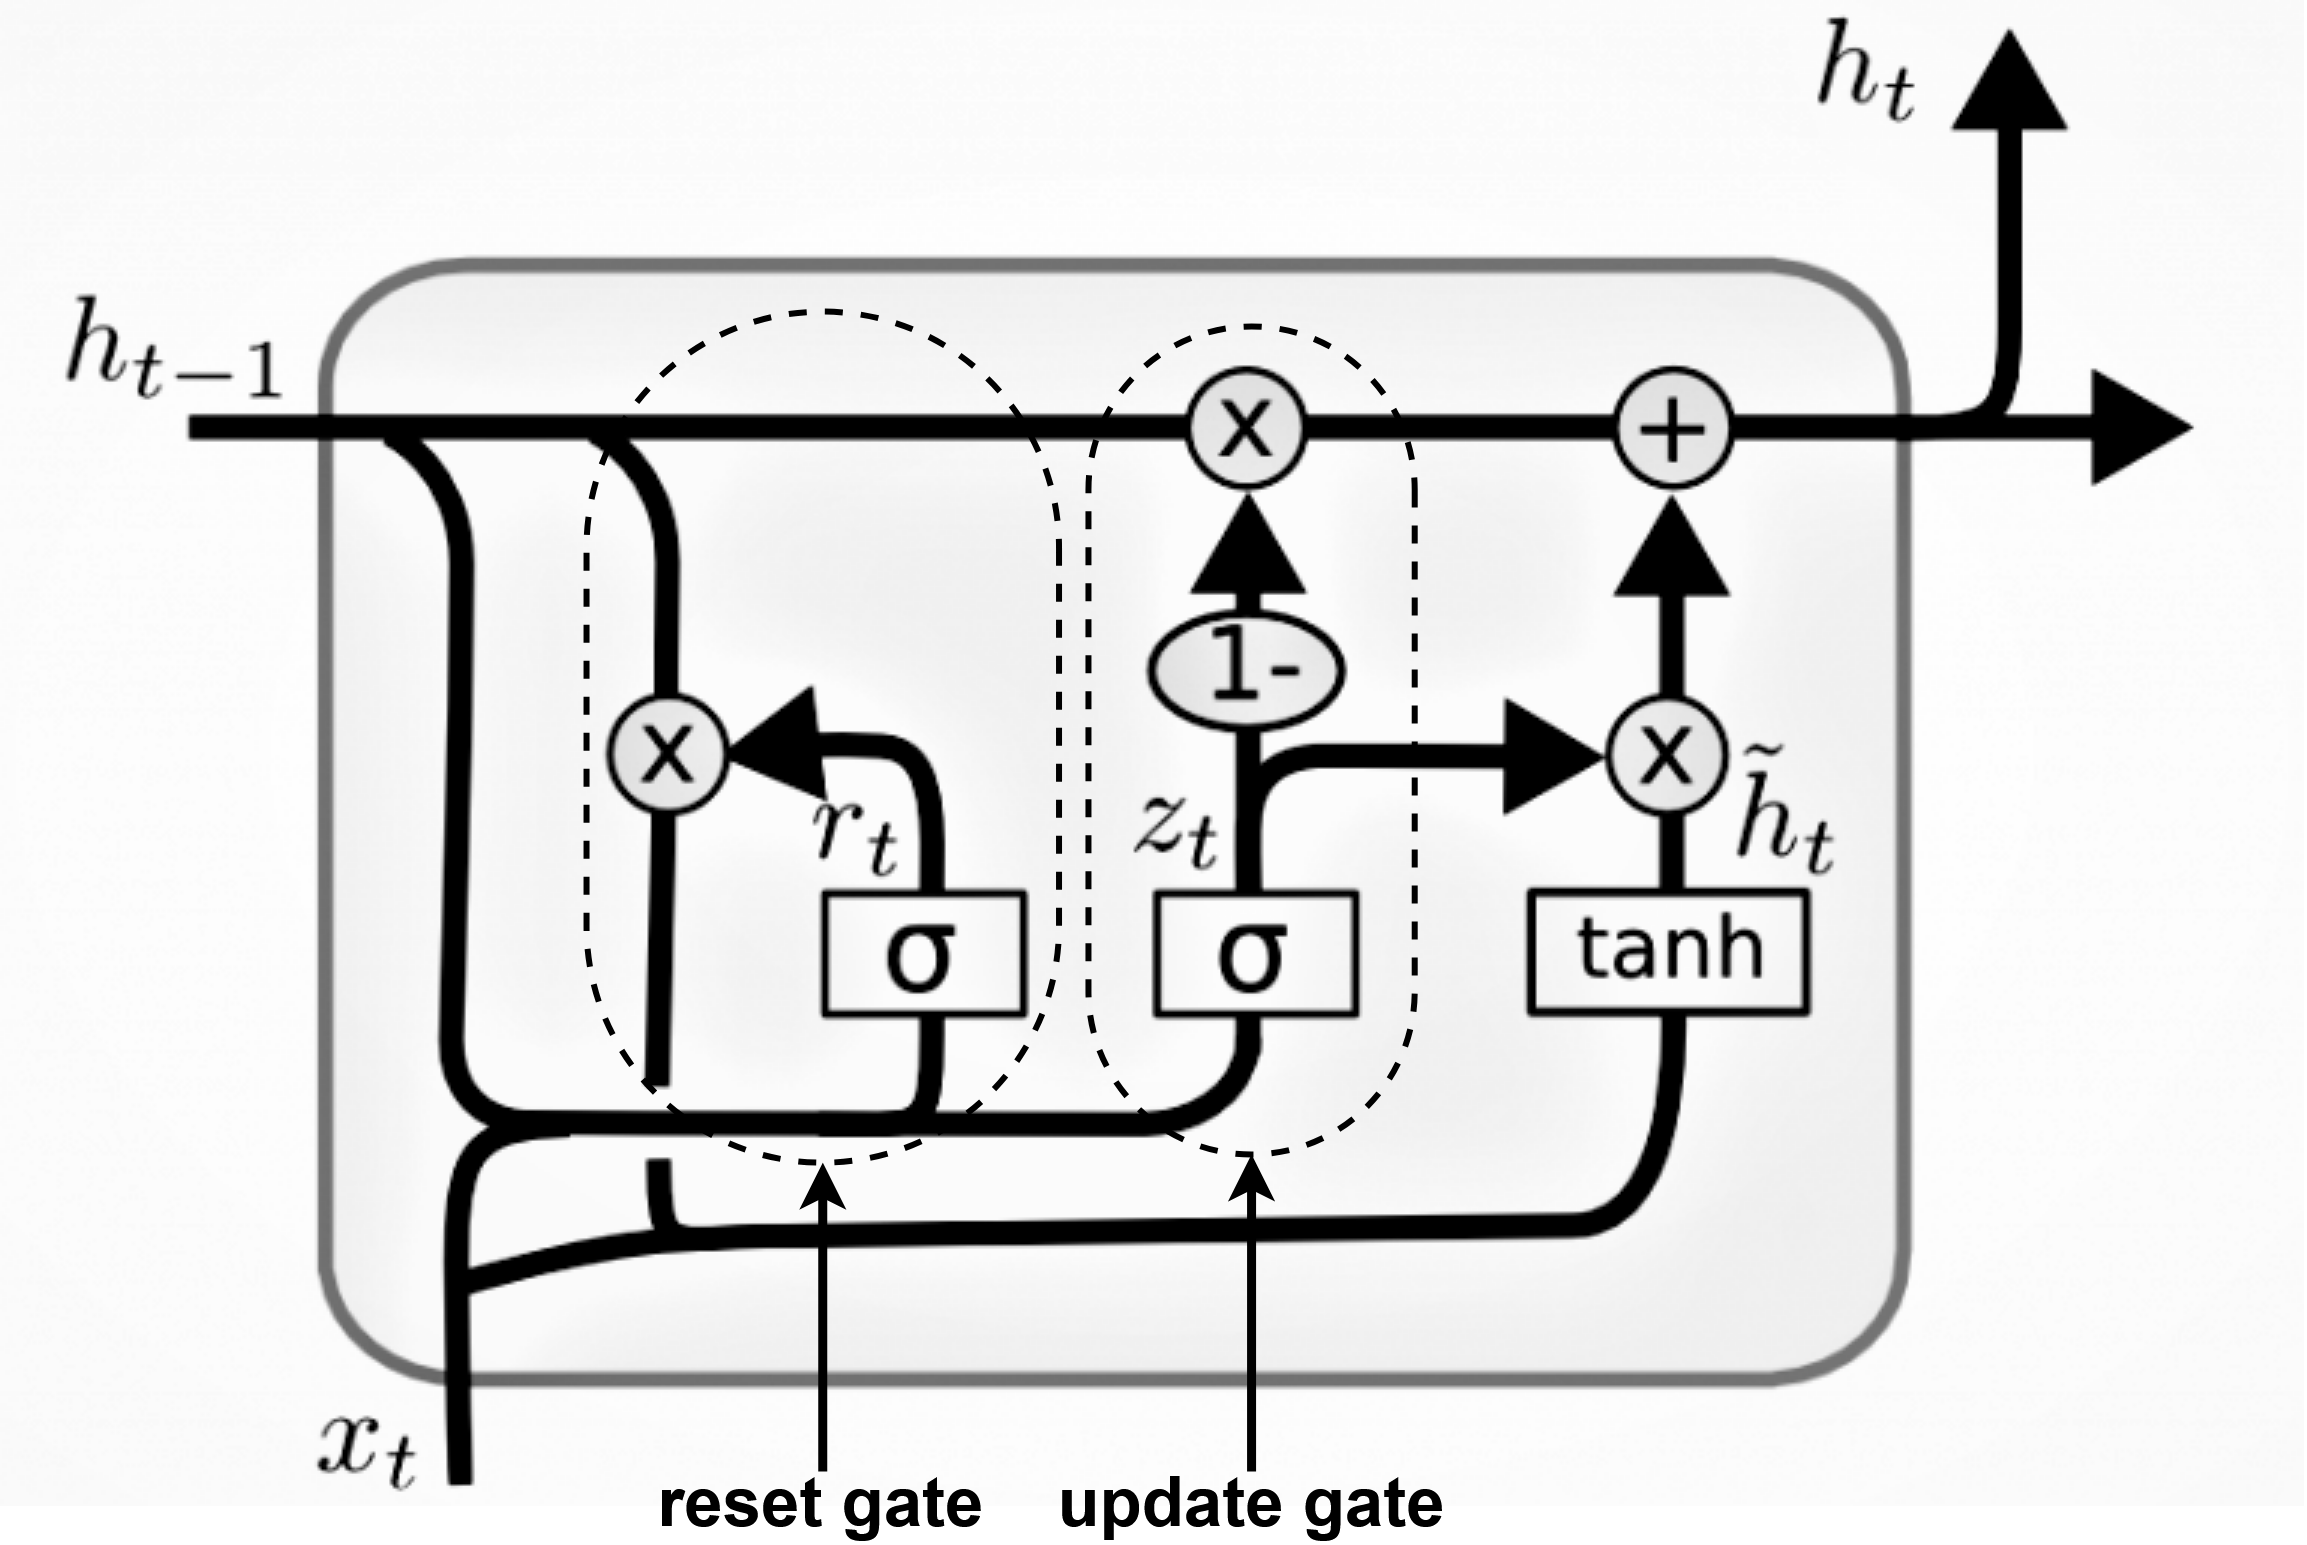
\includegraphics[width=0.6\textwidth]{Images/GRU_cell_detailed.png}
    \caption{GRU unit.}
    \label{gru}
    \end{center}
\end{figure}


The \ac{GRU} structure allows to capture dependencies of large data sequences without discarding information from previous parts of the sequence. This is achieved through its gates, similar to \ac{LSTM}s. These gates are responsible for regulating the information to be kept or discarded at each time interval.

The \ac{GRU}'s ability to maintain a long term memory stems from calculations in the \ac{GRU} unit to produce the hidden state. While \ac{LSTM}s have two different states passed between cells - the cell state, which carries long-term memory, and the hidden state, which carries short-term memory - \ac{GRU}s have only one hidden state transferred between time stages. This hidden state is able to maintain both long term and short term dependencies simultaneously, due to the constraint mechanisms and calculations through which the hidden state and the input data pass.  Like the \ac{LSTM} gates, the gates in the \ac{GRU} are trained to selectively filter out any irrelevant information, keeping what is useful.

These gates essentially produce vectors containing the values 0 or 1 that will be multiplied with the input data and/or hidden state. A value of 0 in the vectors indicates that the corresponding data in the input or hidden state is not important and therefore will be overridden. On the other hand, a value of 1 in the array means that the corresponding data is important and will be used.


The equations that describe the operation of a \ac{GRU} unit are given by 

\begin{equation}
    \begin{cases} 
        
        z_t = \sigma(W^{(z)} x_t + U^{(z)} h_{t-1} + b^{(z)})\\
        r_t = \sigma(W^{(r)} x_t + U^{(r)} h_{t-1} + b^{(r)})\\
        \tilde{h}_t = \tanh(W^{(h)} x_t + U^{(h)} h_{t-1} \circ r_t + b^{(h)})\\
        h_t = (1-z_t) \circ h_{t-1} + z_t \circ \tilde{h}_t

    \end{cases} ,
\end{equation}

where $zt$ represents the update gate vector, $r_t$ the reset gate vector, $\tilde{h}_t$ the candidate activation vector and $h_t$ the output vector. \ac{GRU}s have fewer tensor operations to perform, and so they take less time to train than \ac{LSTM}s.  

\subsubsection{One dimensional convolutional neural network (1D CNN)}\label{chap3:subsubsec:1dcnn}


Convolutional Neural Networks (\ac{CNN}s) are biologically-inspired feed-forward neural networks that have been successfully applied in the field of computer vision and digital image processing and analysis \cite{cnn0}.

In \ac{ML} applications, \ac{2D CNN} are typically used for categorizing 2D images (into classification problems) or creating images (in case of regression-based problems). In this kind of applications, the layers extract two-dimensional pathces from an image and then apply similar transformations to each of the patches. Similarly, there are \ac{1D CNN}, that extract data subsequences from a dimension of the main sequence. This thesis aims to predict the future behavior of certain variables of a single dimension, so that models consisting of \ac{1D CNN}'s layers have been tested.

The \ac{1D CNN} is very effective when you expect to derive interesting features from shorter (fixed-length) segments of the overall data set. Its main purpose is to turn the long input sequence into much shorter (downsampled) sequences of higher-level features, which can be very useful in the treatment of large time sequences.

In Figure \ref{conv1}, the reader may find a representation of the normal working process of a \ac{1D CNN}. The operation of \ac{1D CNN} is based on the extraction of odd size pathces (in this particular case it uses a convolution window with size 5), from a sequence of large dimensions of input data. Is then applied a convolution operation that can be written as \cite{cnn2} 

\begin{equation}
y(n)=
    \begin{cases} 
            
        \sum_{i=-\frac{k}{2}+\frac{1}{2}}^{\frac{k}{2}-\frac{1}{2}} x(n+i)h(i),\  if \  n=0.\\
        \sum_{i=-\frac{k}{2}+\frac{1}{2}}^{\frac{k}{2}-\frac{1}{2}} x(n+i+(s-1))h(i),\  otherwise.\\
    
    \end{cases} ,
\end{equation}

where $n$ represents the length of the convolution layer, $x$ represents the input of the layer, $h$ represents the kernel (or extracted patch) and $k$ its length. Lastly, $s$ represents the number of shifted positions of the kernel window after each convolution, also known as number of strides. For example, if n = 20, k=5 and s=1 then

\begin{equation}
    \begin{cases} 
        y(2)=x(0)h(0)+x(1)h(1)+x(2)h(2)+x(3)h(3)+x(4)h(4)\\
        y(3)=x(1)h(0)+x(2)h(1)+x(3)h(2)+x(4)h(3)+x(5)h(4)\\
        \  ...\\
        y(17)=x(15)h(0)+x(16)h(1)+x(17)h(2)+x(18)h(3)+x(19)h(4)\\
    \end{cases} .
    \label{noncausal}
\end{equation}

It should be mentioned that the output ($o=16$) does not have the same dimension as the input layer ($n=20$). This happens because no padding has been applied to the convolution which implies that for the length of the convolution layer $n$, the kernel size $k$, and the number of strides $s$, the output $o$ is given by:

\begin{equation}
    o = \lfloor \frac{(n-k)}{s} \rfloor + 1 .
\end{equation}

By applying "padding", having the input $n$, kernel size $k$, and padding with length $p$, the output $o$ is given by:

\begin{equation}
    o = \lfloor \frac{(n+2p-k)}{s} \rfloor + 1 .
\end{equation}

This allows to obtain \ac{1D CNN}'s layers whose input size is equal to the output. In this example, for the output $o$ dimension to have the same dimension as the input sequence, 20, then the $p$ dimension must be 2. In Figure \ref{conv1} it can be seen schematically the result of the described convolution operation.

\begin{figure}[h!]
    \centering
    \begin{center}
    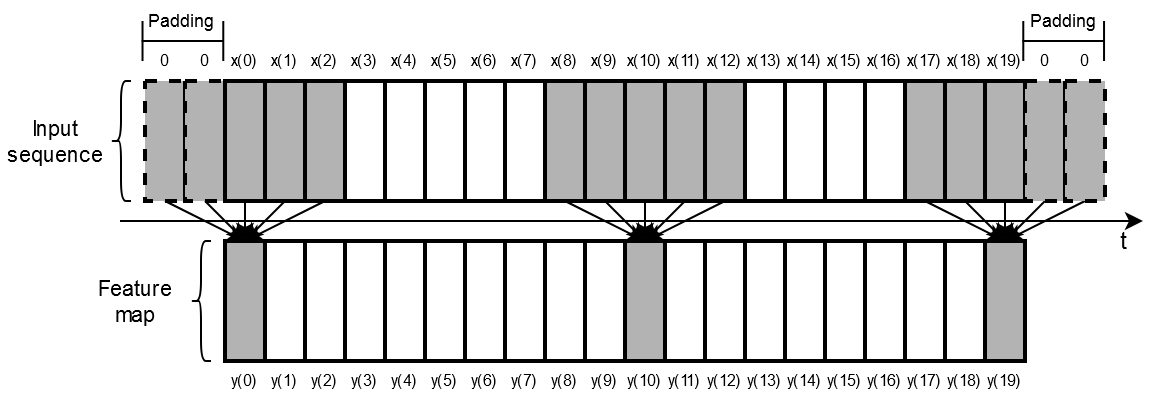
\includegraphics[width=1\textwidth]{Images/conv1.png}
    \caption{1D convolution working process.}
    \label{conv1}
    \end{center}
\end{figure}

Although it may seem like a good methodology, the convolution operation presents a particularity: it uses future values in its computing procedure. In the example present in Figure \ref{conv1}, it can be observed that in the computation of $y(10)$, for example, values of $x(8)$, $x(9)$, $x(10)$, $x(11)$ and $x(12)$ were used. In a series with time dependencies such as the problem in question, the use of future values in the computation of a present value presents an obvious violation, in which the output of instant $[t]$ depends on the input of $[t+1:]$. In this sense, the concept of causal convolution must be introduced. 

In causal convolution, the value of the generated output is not dependent on future inputs. In the same way described above, the causal convolution is given by 

\begin{equation}
y(n)=
    \begin{cases} 
            
        \sum_{i=0}^k x(n-i)h(i),\  if \  n=k-1.\\
        \sum_{i=0}^k x(n-i+(s-1))h(i),\  otherwise.\\
    
    \end{cases} ,
\end{equation}

where $n$ represents the length of the convolution layer, $x$ represents the input of the layer, $h$ represents the kernel (or extracted patch) and $k$ its length. Lastly, $s$ represents the number of shifted positions of the kernel window after each convolution, also known as number of strides. For example, if n = 20, k=5 and s=1 then

\begin{equation}
    \begin{cases} 
        y(4)=x(4)h(0)+x(3)h(1)+x(2)h(2)+x(1)h(3)+x(0)h(4)\\
        y(5)=x(5)h(0)+x(4)h(1)+x(3)h(2)+x(2)h(3)+x(1)h(4)\\
        y(6)=x(6)h(0)+x(5)h(1)+x(4)h(2)+x(3)h(3)+x(2)h(4)\\
        \  ...\\
        y(19)=x(19)h(0)+x(18)h(1)+x(17)h(2)+x(16)h(3)+x(15)h(4)\\
    \end{cases} .
    \label{noncausal}
\end{equation}

In Figure \ref{conv2}, a schematization of the causal convolution process can be seen.

\begin{figure}[h!]
    \centering
    \begin{center}
    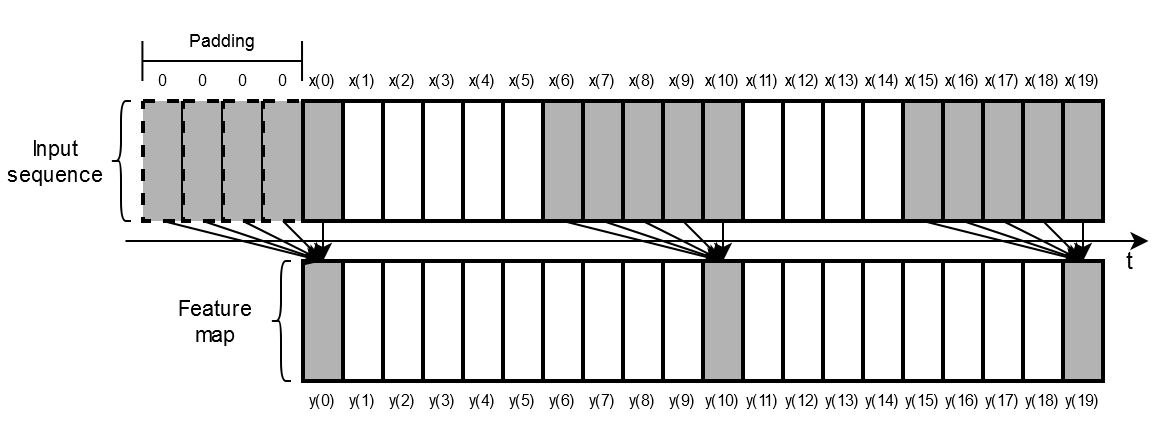
\includegraphics[width=1\textwidth]{Images/conv2.png}
    \caption{1D causal convolution working process.}
    \label{conv2}
    \end{center}
\end{figure}

In this layer category, convolutional windows are used, which is similar to using a k-dimensional kernel where all its elements have the value $\frac{1}{k}$. Following the example, with the kernel described in dimension 5, $y(19)$ is given by
\begin{equation}
        y(19)=x(19)\frac{1}{5}+x(18)\frac{1}{5}+x(17)\frac{1}{5}+x(16)\frac{1}{5}+x(15)\frac{1}{5}.
    \label{19}
\end{equation}



Usually, along with the \ac{CNN} layers, pooling layers are used. The pooling operation aims to simplify convolution output, giving more importance to prominent features and patterns. There are several types of pooling, the most important of which is Max pooling which involves selecting the largest value in a user-defined size window, thus reducing the dimensionality of the output. Following the example, for a $pool\_size$ of 5 units, one can see in Figure \ref{maxpooling}, the representation of the Max pooling operation where the dark units have the highest value within the 5-unit window. For the first 10 time-setps, the highest value value is then passed as layer output, and the dimension of the output decreases. In other words, for each set of 5 values, the largest is chosen, and the size of the output decreases with an inverse relationship to the chosen $pool\_size$. In this case, the dimensionality of the output decreases five times.

\begin{figure}[h!]
    \centering
    \begin{center}
    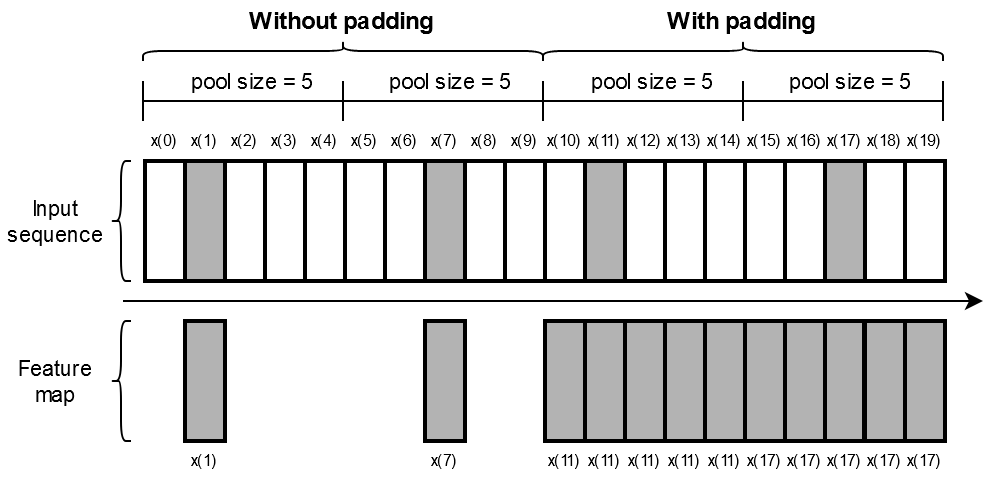
\includegraphics[width=0.9\textwidth]{Images/maxpooling.png}
    \caption{Max pooling without and with padding.}
    \label{maxpooling}
    \end{center}
\end{figure}

If the user intends to apply a normal pooling process, there is an obvious reduction in dimensionality. If you one intends to extract the most relevant features while maintaining the same dimensionality, it is also possible. To accomplish this, padding should also be added to this layer. In Figure \ref{maxpooling}, for the last 10 time-steps, it is possible to observe Max pooling with padding, where the beginning of the process is similar as pooling without padding, but inside the output windows of dimension $pool\_size$, the higher selected value is copied to all the remaining empty spaces. 

In order to aggregate all the information entered regarding the layers {1D CNN}, a simple example is shown in Figure \ref{resdata}, which illustrates the process of convolution between a simple size 5 kernel and a random time signal.

\begin{figure}[h!]
\captionsetup[subfigure]{position=b}
\centering
\subcaptionbox{\label{inputseq}}{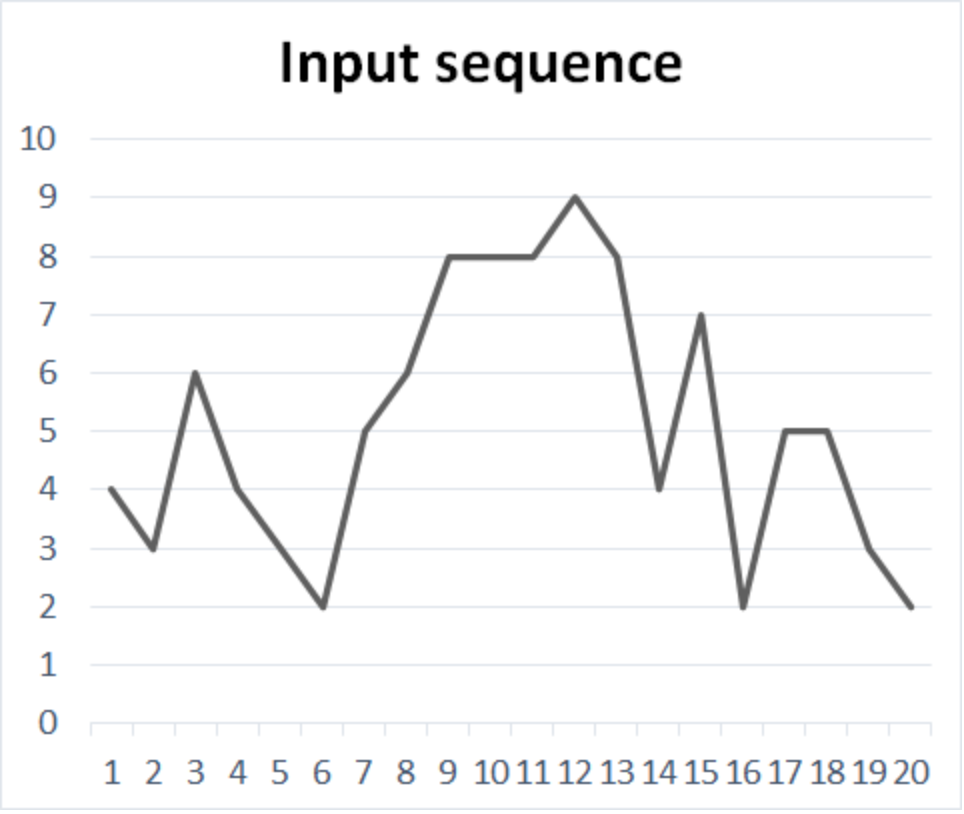
\includegraphics[width=.32\linewidth]{Images/inputsequence.png}}
\subcaptionbox{ \label{afterconv}}{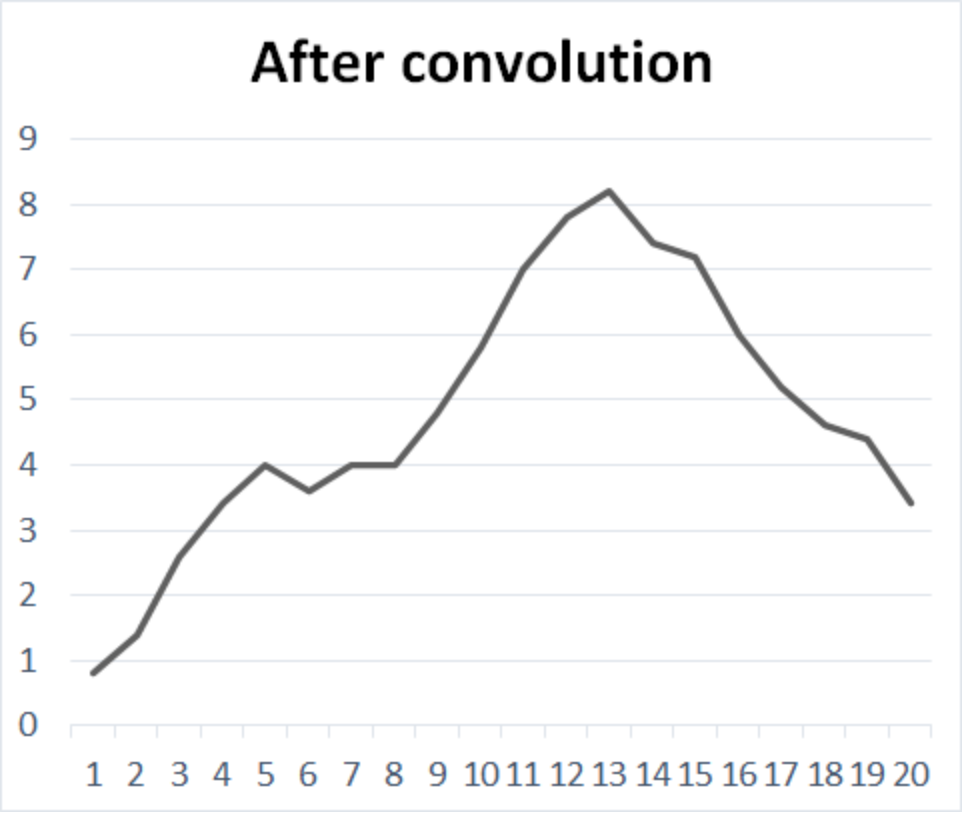
\includegraphics[width=.32\linewidth]{Images/afterconvolution.png}}
\subcaptionbox{ \label{aftermaxp}}{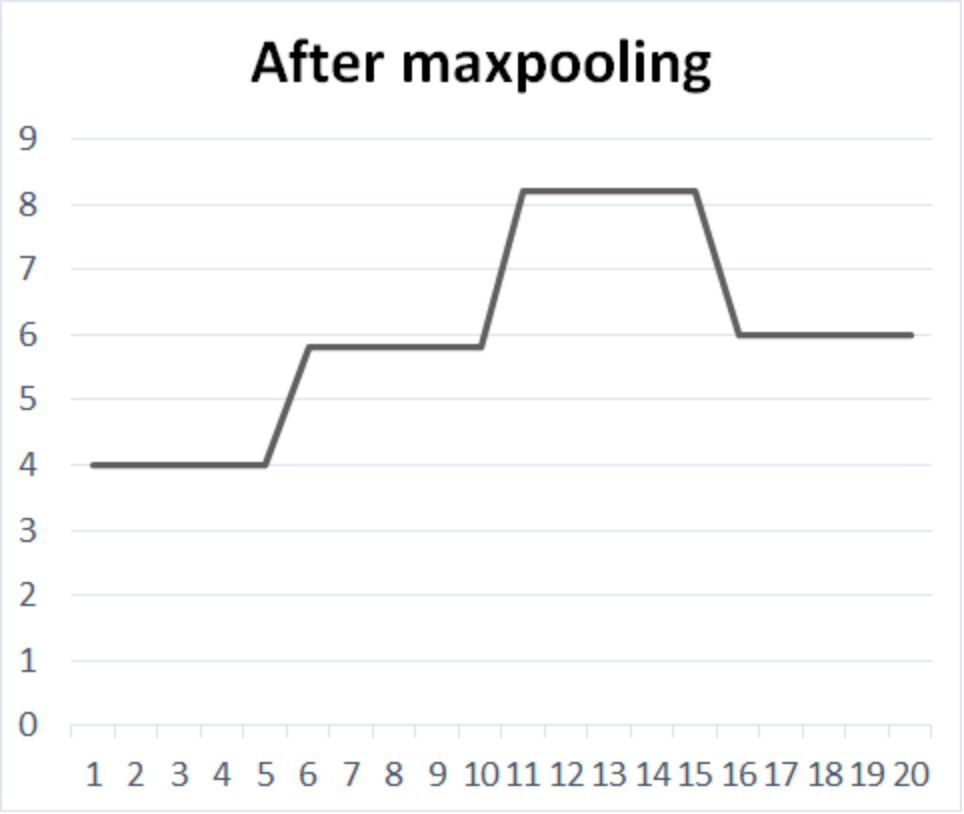
\includegraphics[width=.32\linewidth]{Images/aftermaxpooling.png}}
\caption{Example data a) Before convolution b) after convolution c) after Max pooling.}
\label{resdata}
\end{figure}


Figure \ref{inputseq} shows a 20 time-steps random signal, as the one used in the other examples used in this section. At this stage, the signal is in its original form, without any treatment. Figure \ref{afterconv} represents the result after the convolution operation with kernel\_size 5. It can be seen that at this point, the signal is a smoothed representation of the initial signal. The convolution operation extracts the main characteristics of the signal, ignoring intermediate oscillations. Afterwards, the Max pooling operation with pool\_size 5 is applied to the signal resulting from the convolution operation. The result of this operation is represented in Figure \ref{aftermaxp}. In red, is the result of the operation of Max pooling without padding, where the main points of the sequence are extracted, thus reducing the dimensionality of the time series. In grey, the same operation can be observed but with padding,  which consists of extending the point with the highest value within each of the 4 defined windows. This is the final signal resulting from the convolution operation with Max pooling, a simplified representation of the initial sequence. It is important to point out that the process described is a very simplified representation of the way the layers \ac{1D CNN} work. In practice, this process is much more complex, and is carried out taking into account multiple variables simultaneously. A more detailed description of this process will be provided later on. 

\subsection{Networks specifications}\label{chap3:subsec:networks_specifications}

The process of designing the architectures to be tested is a complex and demanding task. This section describes the architectures used, as well as some techniques used in their development.

\subsubsection{Studied architectures}\label{chap3:subsubsec:studied_architectures}
In the development of this thesis, different types of neural networks were tested, composed of the layers introduced in section \ref{chap3:subsec:artificial_neural_networks}. The objective was to study the influence that each of the three layers introduced has on a predictive model, and to study the results obtained by pairing multiple layers into a single model. 

\paragraph{Vanilla architecture}

The first architecture proposed for this study is a simple architecture, based on the many-to-one concept, which consists of using the input features of the last instants to predict a single value in the future. 
In Figure \ref{arc1} one can see an illustrative scheme of how this architecture works.

\begin{figure}[h!]
    \centering
    \begin{center}
    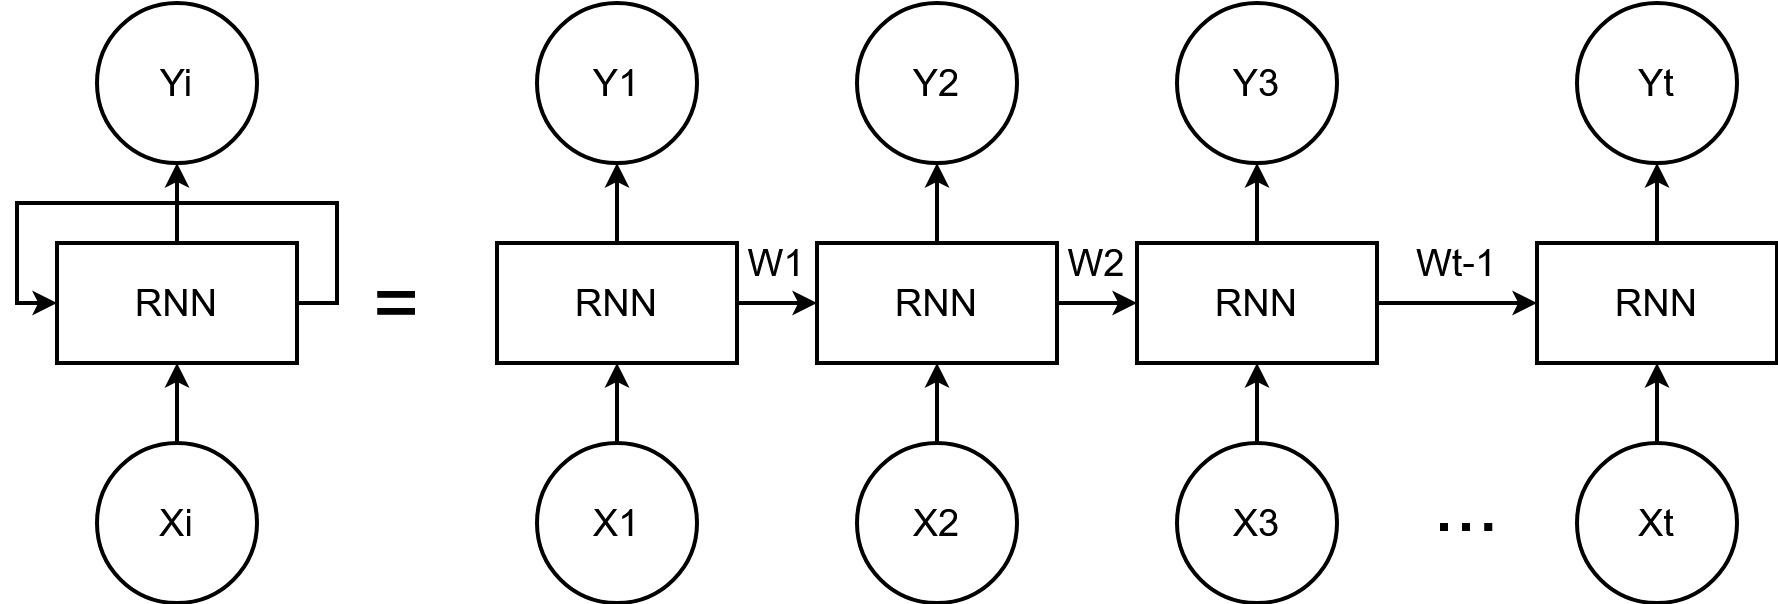
\includegraphics[width=0.7\textwidth]{Images/arc1.png}
    \caption{Vanilla architecture}
    \label{arc1}
    \end{center}
\end{figure}

This is a very common architecture that uses the capacity of the \ac{RNN}s to predict a single future value of the sequence. In Figure \ref{arc1}, one can see the working mode of the architecture where on the left side there is a representation of the functioning of a RNN cell, and on the right side there is a more detailed representation of the functioning of that same cell. As explained in section \ref{chap3:subsec:artificial_neural_networks}, there are two types of cells \ac{RNN} that present this type of behavior, the cells \ac{GRU} and \ac{LSTM}. In this sense, two models have been created, Model 1.1 whose architecture is similar to the structure presented in Figure \ref{arc1} and uses cells of type \ac{GRU}, and Model 1.2 whose architecture is similar but uses cells \ac{LSTM}. A relevant point to mention is that, as can be seen in Figure \ref{arc1}, for each $yt$ a $yt$ is generated. In this case, it is intended to forecast three values with a many to one architecture. The problem was modeled so that $yt$ corresponds to a vector $yt = [y(t+5), y(t+10), y(t+15)]$, that is, the vanilla model was adapted to produce an output with three values at each iteration. For this purpose, all the three supervised learning series, defined in section \ref{chap3:subsec:data_shifting}, were used.



\paragraph{Encoder-Decoder architecture}

The second proposed architecture is known as Encoder-Decoder.  This is a many-to-many architecture, that is, from a past data sequence, the architecture is able to predict a new data sequence. Contrary to the previous architecture, which produced only one value per iteration, this architecture uses the values up to instant t to produce data sequences for the next $N$ steps $(t+1, t+2, ..., t+N)$. This architecture is then more suitable in the context of this problem, since it can be used to predict for each instant t, the next 15 steps $(t+1, t+2, ..., t+15)$. In Figure \ref{arc3}, a schematic representation of the functioning mode of the Encoder-Decoder architecture can be observed. 

\begin{figure}[h!]
    \centering
    \begin{center}
    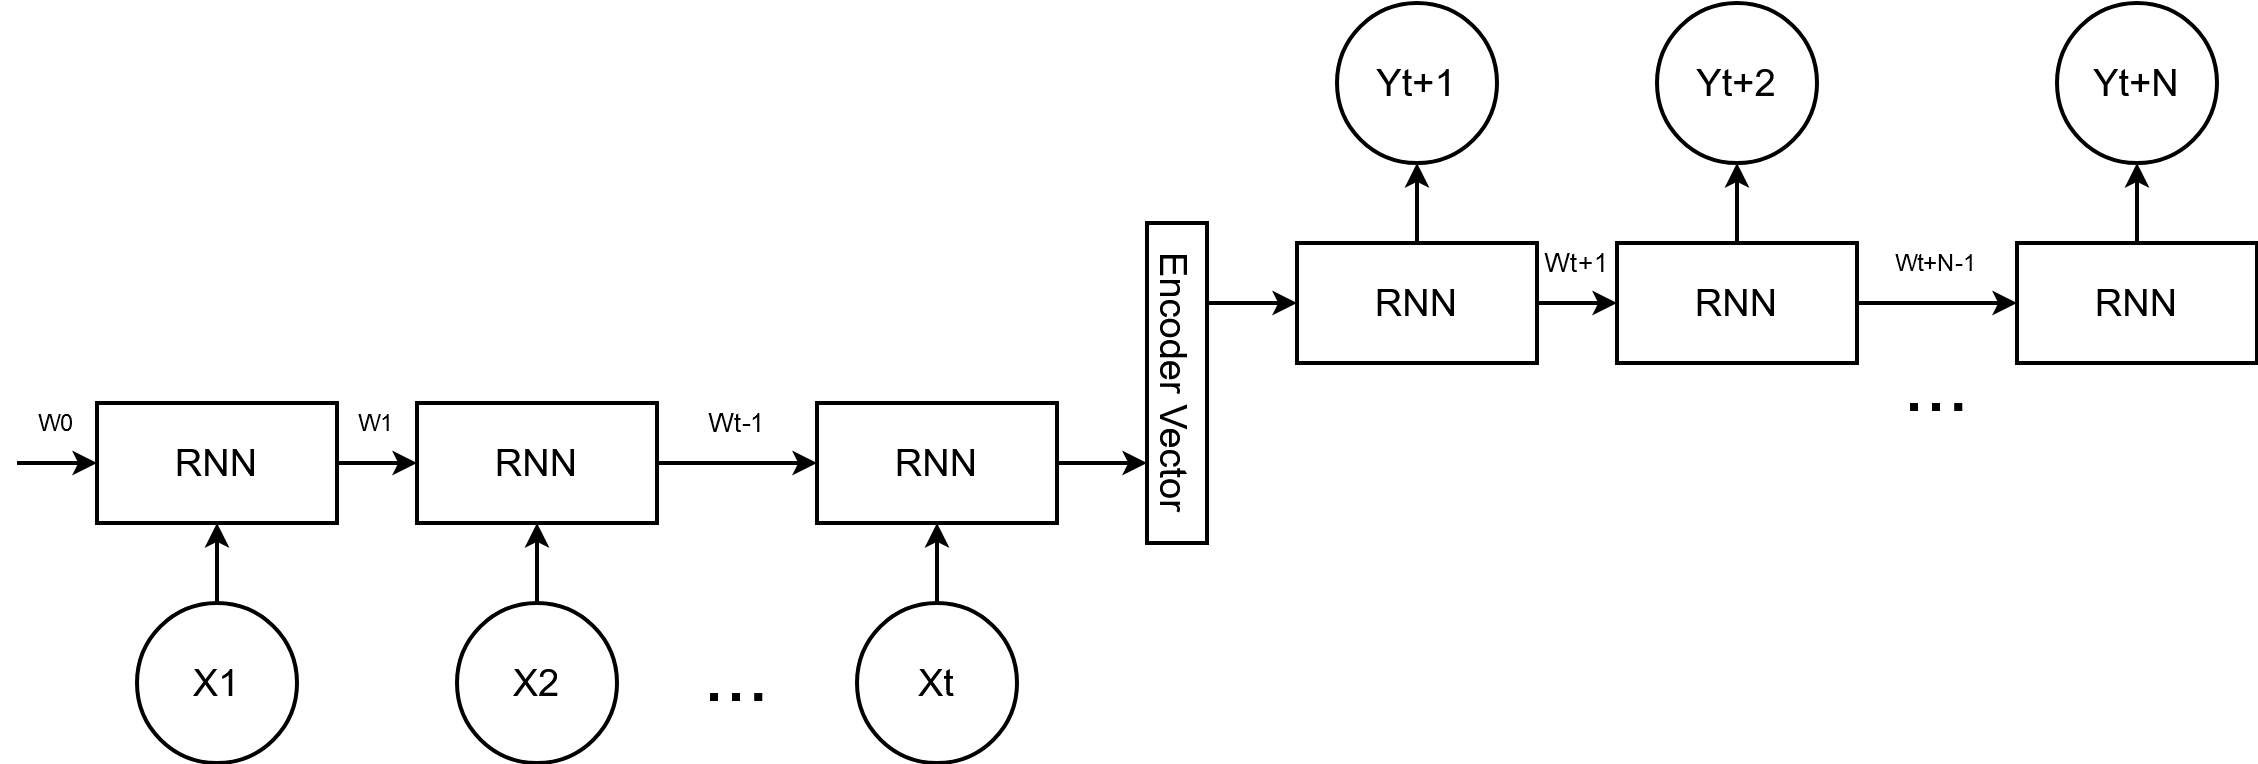
\includegraphics[width=0.9\textwidth]{Images/arc2.png}
    \caption{Encoder-Decoder architecture}
    \label{arc2}
    \end{center}
\end{figure}

As can be seen in Figure \ref{arc2}, this architecture is subdivided into two levels. The encoder level, present on the left, and the Decoder level, present on the right. The encoder is composed of a set of recurrent cells, responsible for aggregating important information about the input in the encoder vector. The decoder, present on the right side of the Figure \ref{arc2}, is responsible for using the information present in the encoder vector to make a forecast for the next N steps. It can also be seen that the output of the first step of the decoder is entered as input for the production of the next value of the sequence, and so on. This is a fundamental feature that enhances the production of the sequence. As in the Vanilla architecture, the Encoder-Decoder architecture has been implemented with two types of cells, \ac{GRU} which refers to Model 2.1 and \ac{LSTM} which refers to Model 2.2. Since this one is a many-to-may architecture, none of the sequences defined in section \ref{chap3:subsec:data_shifting} could be used for this model. For this purpose, sequences had to be developed\footnote{Both the code of this step as well as the rest of the developed code can be found at} that took into account both the size of the input sequence and the output sequence.



\paragraph{1D CNN Encoder-Decoder architecture}


The third architecture proposed is similar to the Encoder-Decoder architecture, but in this case the encoder, instead of being formed by a \ac{RNN} similar to the Decoder, is formed by a \ac{1D CNN}. Using the \ac{1D CNN} as an encoder may bring some advantages, namely the ability of this type of layers to identify small patterns in the input data.  As its name indicates, the \ac{1D CNN} layer applies the process of convolution between two functions, determining the relationship between them. The integral of this convolution, in turn, expresses how the form of a function is altered by the form of another function. This type of network is usually used in image processing, but by applying it to signals of only one dimension, as is the case with the input features available for the model to be developed, it is possible through the convolution process to identify how small patterns in one feature can affect the others. For this reason, it is then possible to combine this capacity if \ac{1D CNN}s with the predictive capacity of \ac{RNN}s from a hybrid model Encoder-Decoder. In Figure \ref{arc3}, the reader can find a diagram illustrating the operation mode of the Hybrid Encoder-Decoder model.

\begin{figure}[h!]
    \centering
    \begin{center}
    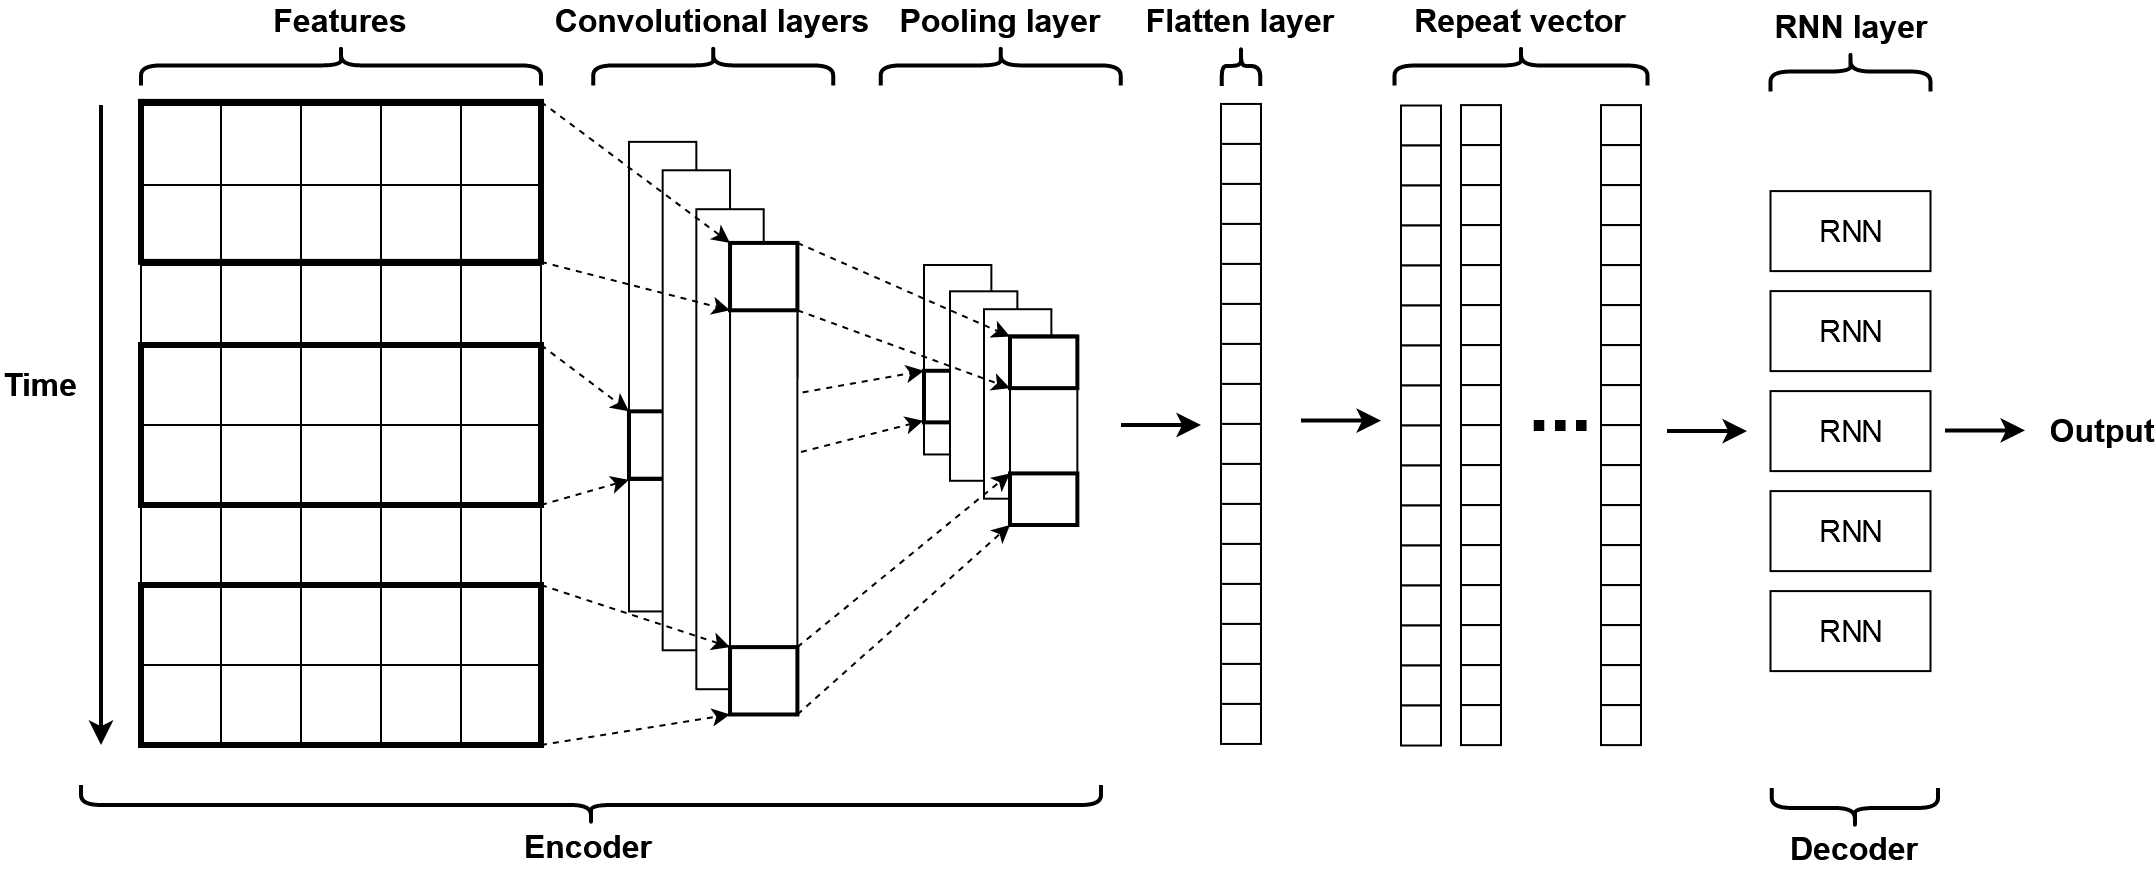
\includegraphics[width=1\textwidth]{Images/ED.png}
    \caption{1D CNN Encoder-Decoder architecture}
    \label{arc3}
    \end{center}
\end{figure}

By examining Figure \ref{arc3}, one can see how the third architecture proposed works. Given a temporal sign where the length represents the number of timesteps and the width the number of variables in a multivariate temporal series, the convolution kernels, with the same width as the temporal series, are sliding windows of defined length that travel through the temporal series performing the convolution process. The kernel elements are multiplied by the elements of the time series that they pass through at each instant. Then, the results of the multiplications are added together and a non-linear activation function is applied to the resulting value. As a result of the whole process, an element of an univariate time series is obtained. Then the kernel moves down one position and this process is repeated, generating the second value of the univariate time series. This is the process performed by a kernel. The number of univariate time series obtained corresponds to the number of kernels used. A set of univariate time series is then obtained which can be said to be "filtered". The second stage involves carrying out the Pooling process with each time series where the largest or the largest values are selected. A new vector, of smaller dimension, is then formed for each series. Then, all the vectors are flattened generating a single vector of larger dimension. This vector corresponds to the encoder vector detailed in Architecture 2. From this point on, the process is similar to the previous architecture. 

As in the other architectures, this architecture can be divided into two models, Model 3.1 where the recurring cells are \ac{GRU}s, and Model 3.2 where the reoccurring cells are \ac{LSTM}s. 



%In Figure \ref{models}, are represented the five main architectures studied.

%\begin{figure}[h!]
%    \centering
%    \begin{center}
%    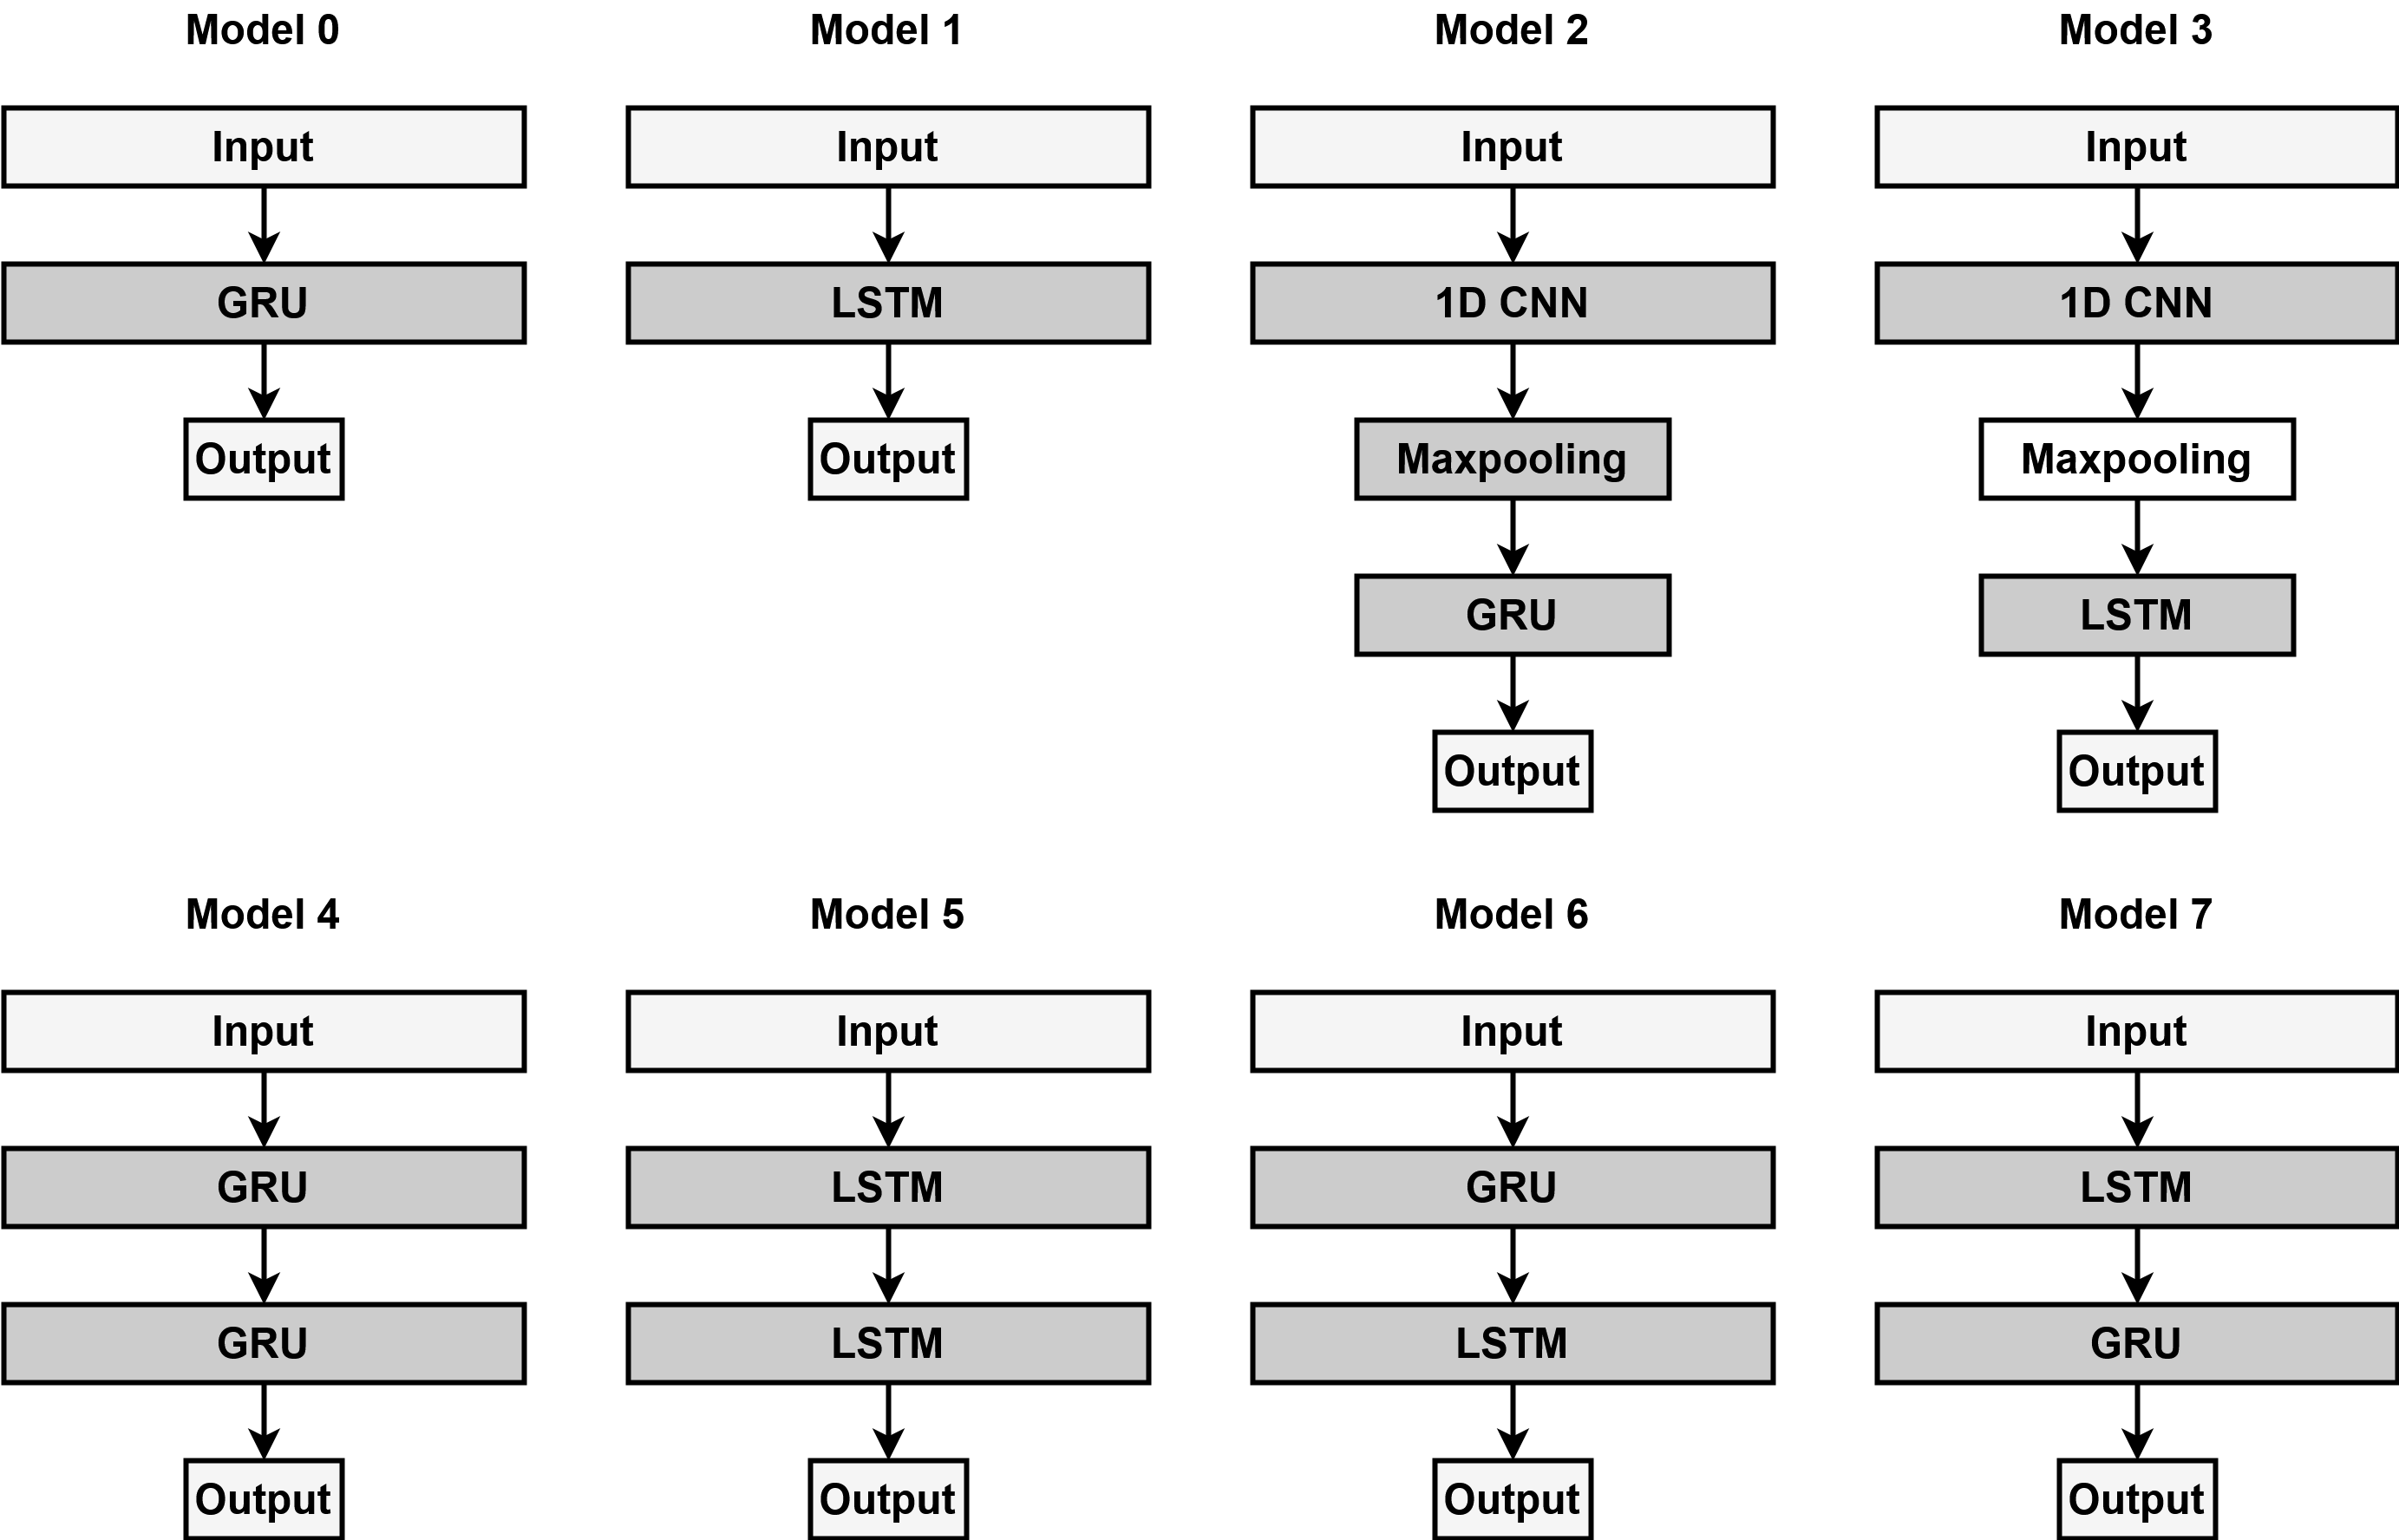
\includegraphics[width=1\textwidth]{Images/models.png}
%    \caption{Tested model architectures.}
%    \label{models}
%    \end{center}
%\end{figure}

%Model 1 and Model 2 are composed of a single layer of \ac{GRU} and \ac{LSTM} respectively. The purpose of these two models is to compare the performance between the two types of single layer. These two models were chosen, because both architectures are already known to perform well when it comes to time series forecasting problems. So one has a set of two simple models with predictive capabilities. These two models use as input all the variables selected through the \ac{ac} process based on the assumption that all the features help to predict the target, the Available Power of the building in the feature. 

%Although the \ac{PCA} procedure detailed in section \ref{chap3:subsec:feature_selection}, which defined the best features to be used as inputs of the selected models, it was decided to test the models with a single input feature, the past Available Power. The reason behind this choice is that it is suspected that a more complex model that has access to a larger number of features can also be easily deceived by those features. Once there is access to past measurements of the variable to predict, it was also experimented to use only this variable as an input feature. Models 3 and 4 present an architecture quite similar to the architecture of models 1 and 2, with the slight difference that only the past records of the output variable are used as input, i.e., with input only the measure of available power is given, and as output is expected the future value of available power and 5, 10 and 15 minutes. The study of these two models aims to evaluate simpler models with access to fewer variables, and compare their performance with models 1 and 2 that use all the features they have available to meet all the necessary requirements. Although the best 13 input variables from a set of 70 have been defined, nothing guarantees that the use of the larger set of variables will produce better results than the introduction of only past values of the variable to be predicted. 

%The layers \ac{1D CNN} layers introduced in section \ref{chap3:subsubsec:1dcnn}, thanks to their mode of operation, are often used for feature extraction on input data, since they have the ability to identify patterns in the input features. By combining this capability with the capability of \ac{GRU} and \ac{LSTM}s to support sequence prediction, it is hoped to obtain more capable models for predicting the proposed variable. In order to study the effect that the combination of \ac{CNN}s with \ac{GRU}s and\ac{LSTM}s has, the architecture of model 5 is similar to that of model 3, with the addition of a set of \ac{1D CNN} layers, and a Maxpooling layer before the \ac{GRU} layer. Similarly, model 6 is like to model 4 with the addition of a set of \ac{1D CNN} layers and a Maxpooling layer before the \ac{LSTM} layer. 

%All six architectures present, as their last layer, a Dense layer with three units, responsible for converting the outputs of the previous layers into only three outputs, one for each of the forecasts ((t+5), (t+10) and (t+15)). There are a total of two multivariate models, which use all the variables selected as input features, two similar models but using only one input feature, and two hybrid models with combine the capabilities of convolutional networks with the predictive capabilities of the models proposed so far. 


\subsubsection{Data standardization}\label{chap3:subsubsec:data_standardization}

As mentioned in section \ref{chap3:subsec:feature_selection}, there are several features that can be used in the implementation of \ac{ML} methodologies, namely in the use of \ac{ANNs}. Besides the several features have different scales, the \ac{ANNs} have a better performance when the data is standardized. Also, if inputs are not limited to a range like (0.1) or (-1.1) the model used will have difficulty in equally distribute importance of each feature, thus naturally large values become dominant relatively smaller values during the training of \ac{ANNs}.

From mod to avoid this kind of failures, a $MinMaxScaler$ \ref{minmax} was applied, whose mode of operation consists in transforming each feature individually, scaling it to a given interval(by default (0.1)).  Arithmetically, this function is given by

\begin{equation}
     X_i' = \frac{X_i - min(x) }{max(x)-min(x)},
\label{minmax}
\end{equation}

where $X_i'$ represents the rescaled value, $X_i$ the original value, $min(x)$ is the minimum value in the specific feature, and $max(x)$ is the maximum value in the feature. The standardized feature is then obtained in the defined range. Usually, this process consists of two phases, a phase in which the scaler used is adapted to the data and a phase in which it is used to transform the data. It is good practice to use the training data to adapt the scaler and transform the data, and the test data are only transformed. This reduces the bias associated with transforming unknown data. The inverse process to that presented in the equation \ac{ANN} is applied to the output of the \ac{ANN}, in order to transform the data back to its original scale.



\subsubsection{Hyperparameter optimization} \label{chap3:subsubsec:hyperparameter_optimization}

A hyperparameter is a parameter whose value is used to control the learning process. Hyperparameter optimization is the process of choosing a set of optimal hyperparameters for a learning algorithm. Depending on the layer in question, different hyperparameters can be tuned. Other parameters, such as node weights are initialized randomly, and are defined during the learning process. In other words, hyperparameters are parameters which must be changed by the user according to the results obtained, while other parameters should not be modified by the user, and are the result of the learning process.

\ac{ANN}s have numerous advantages, both in terms of their usage and performance. On the other hand, tuning the hyperparameters is an extremely time-consuming process that is done by hand. A certain set of hyperparameters is trained, validated, and then changed and so on until the best possible result is obtained. During the validation phase, different hyperparameters were tuned such as the number of nodes in each layer, number of filters of each \ac{1D CNN} layer and kernel size. Exhaustive grid search, a brute-force technique, was then used, which consists in testing all possible combinations of a hyperparameter user-defined grid. For each combination and hyperparameters, the models were evaluated using the validation methodology introduced in section \ref{chap3:subsec:data_partition}. This way, it was possible to obtain the best combination of hyperparameters for the available data set.

\subsubsection{Regularization techniques}\label{chap3:subsubsec:regularization_techniques}

During the learning process of an \ac{ANN}, it is possible that overfitting occurs. Overfitting is a term used to describe when a model fits very well to the previously observed data set, but proves to be ineffective in predicting new results. In practice, overfitting causes the model to perform very well during training, but the performance gets much worse when faced with brand new data because the model has adapted too much to the training data.  

Regularization refers to a set of different techniques that lower the complexity of a neural network model during training, and thus prevent the overfitting \cite{reg0}. There are several types of regularization techniques. In this thesis, two techniques were used: Early-stopping and Dropout.

\paragraph{Early-stopping}\label{sec:early}

Early-stopping is probably the most common regularization technique. In Figure \ref{early} the reader can find a two graphs that portray the evolution of the error over epochs of a prediction model. During the training and validation process of the predictive models, the error associated with the training set tends to decrease with the increase of the number of training epochs. In an optimal case, with the increase of the number of validation epochs, the error associated with the training set also tends to decrease, thus reaching a trained and validated model whose error produced at validation is minimal. In the case of datasets large enough to overfit, it is observed that most of the time the training set error also tends to decrease, but the validation error starts to increase at a certain point. This is one of the main ways to identify overfitting.

\begin{figure}[h!]
\captionsetup[subfigure]{position=b}
\centering
\subcaptionbox{\label{early0}}{
\includegraphics[width=.45\linewidth]{Images/early-stopping0.png}}
\hspace{0.05\textwidth}
\subcaptionbox{ \label{early1}}{
\includegraphics[width=.45\linewidth]{Images/early-stopping1.png}}
\caption{Prediction error evolution over epochs a) without overfitting b) without overfitting.}
\label{early}
\end{figure}

In Figure \ref{early0}, an ideal case is represented where there is no overfitting. It can be verified that the evolution of the validation error follows the evolution of the training error. Figure \ref{early1} presents a clear case of overfitting in which, at the moment marked with the black dot, the model presents its smallest validation error, which later increases. The early-stopping process consists in, from the moment the system detects that the validation error increases, it runs for more $p$ (patience factor) epochs where it gives the system the opportunity to obtain lower values of validation error. If in none of the $p$ epochs a lower value is found, the training process ends, eraly-stopping occurs. In the extreme case where $p$ = 0, the system stops the training process as soon as it detects a higher value than the previous one for the validation error, moment marked by the black circle present in Figure \ref{early1}.

\paragraph{Dropout}

In the process of training a fully connected \ac{ANN}, neurons tend to develop an interdependence between each other, which limits their individual capacity leading to overfitting.


To tackle this problem, the dropout is used, which is also widely used regularization technique. In Figure \ref{drop0} it is possible to see a \ac{ANN} without a dropout, and in Figure \ref{drop1} it is possible to see the same \ac{ANN} after dropout is applied.

\begin{figure}[h!]
\captionsetup[subfigure]{position=b}
\centering
\label{fig:drop}
\subcaptionbox{\label{drop0}}{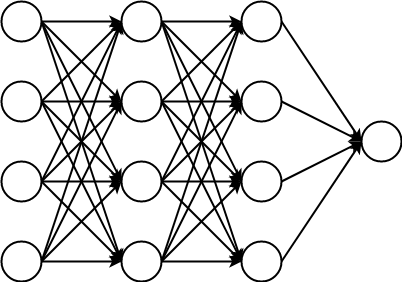
\includegraphics[width=.4\linewidth]{Images/dropout0.png}}
\hspace{0.05\textwidth}
\subcaptionbox{ \label{drop1}}{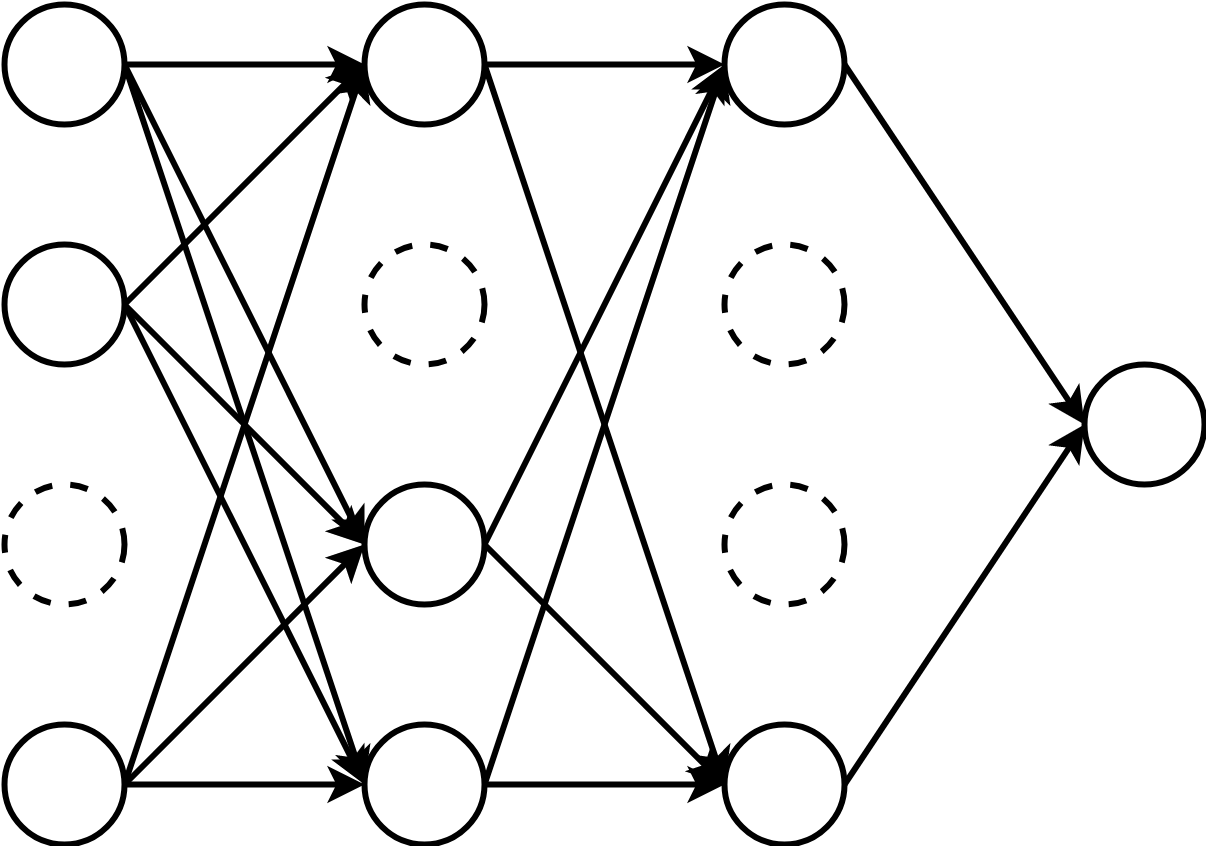
\includegraphics[width=.4\linewidth]{Images/dropout1.png}}
\caption{Artificial neural network a) without dropout b) with dropout.}
\end{figure}

The application of dropouts, implies for each hidden layer, for each sample of training, and for each iteration, to ignore a fraction $p$ of random neurons (and corresponding activations) during the training process. During the validation phase, all activations are then used, but reduced by a $p$ factor to take into account the missing activations lost during the training \cite{drop0}.

\section{Implementation environment}\label{chap3:sec:implementation_enviromnet}

During the development of the thesis, several scripts were implemented, both for data processing and for the implementation of machine learning models. The language chosen for this purpose was \textit{Pyhton}. The primary reasons for this choice were the ease of syntax of this language, as well as the large number of libraries available, including \textit{keras}, a Deep Learning library that provides all the necessary tools for building and deploying Neural Networks.

Regarding the hardware components used, two different systems were used during the development of this work. The first environment consists of a CPU (Intel Core i5-3470 3.20GHz), and a GPU (NVIDIA GeForce GTX 1050 Ti) essential to accelerate the training process of the proposed models. The second environment consists of a virtual environment implemented on \textit{Microsoft Azure Machine Learning} platform, where a cluster consisting of a 6 core processor, and a GPU (NVIDIA Tesla K80).

The first setup was used with the purpose of testing, in a first phase, several models with simple tasks, and the second environment was used to put into practice more complex tests that required more computational capacity.
	
\section{Performance evaluation metrics}\label{chap3:sec:performance_evaluation_metrics}

In the previous section, important details concerning the data used in this thesis were explained. One defined $Model\ error$, but did not specify which concrete metrics were used in this work. To compare the performance of the different models in the defined dataset, it is necessary to use some measures of forecast performance. In this sense, during this thesis four different measures were used that relate the real values present in the time series represented by $y_t$, and the forecast values, which are represented by $f_t$. Thus, the forecast error is given by $e_t=y_t-f_t$. The three measures presented are quite common in the literature \cite{errors} and are described below.

\subsection{Mean Absolute Error (MAE)}

The \ac{MAE}, is defined as

\begin{equation}
     MAE =\frac {\sum_{t=1}^n|e_t|}{n}.
\label{mae}
\end{equation}

The \ac{MAE} is known as a scale-dependent accuracy measure and measures the average absolute deviation between the forecasted values and the real ones. As a scale-dependent measure, it cannot be used to compare series series using different scales.


\subsection{Mean Squared Error (MSE) and Root Mean Squared Error (RMSE)}

The \ac{MSE}, is defined as

\begin{equation}
     MSE =\frac {1}{n}\sum_{t=1}^ne_t^2.
\label{mse}
\end{equation}

The \ac{MSE} is also known as a scale-dependent accuracy measure and measures the average squared deviation between the forecasted values and the real ones. The application of this measure is quite relevant because it doesn't allow the negative errors to cancel the positive errors and vice-versa. 

By applying the square root to the \ac{MSE}, the \ac{RMSE} is then defined as

\begin{equation}
     RMSE =\sqrt{MSE} = \sqrt{\frac {1}{n}\sum_{t=1}^ne_t^2}.
\label{rmse}
\end{equation}
Mathematically, the \ac{RMSE} is the square root of the average of the squared difference between the predicted values and the observed ones. The advantage of \ac{RMSE} over \ac{MSE} is that it is on the same scale as the targets, facilitating its interpretation in the concrete context of the problem. 

\ac{RMSE} and \ac{MAE} were the metrics implemented in the development of this research. These two measurements present some similarities, but also some differences that make it relevant to use the two metrics separately. In terms of similarities, both are expressed in the units of the variable in question, which means that both errors are easily interpretable given the context of the problem. The major difference between the two metrics lies in the contribution that individual error values make to the final result. In the case of \ac{MAE}, the contribution of individual errors follows a linear behavior. An error of 20 units contributes twice as much as an error of 10 units, and an error of 500 units contributes half as much as an error of 1000 units. In the case of \ac{MSE} the errors are squared before being averaged, which means that this metric gives more weight to larger errors.  This means that very small errors tend to be ignored while large errors tend to be magnified. One can then conclude that \ac{MSE} is especially useful when one intends to emphasize large errors and reduce the importance of smaller error. This is why this was the metric chosen as loss\_function, since by emphasizing large-scale errors, they end up being penalized, which is quite useful in time series, where the intention is to avoid this type of failure as much as possible. It was also decided to calculate, for all training, validations and tests, the \ac{MSE} and the \ac{MAE}. The first one because it translates the \ac{MSE} to the scale of the problem, allowing a better interpretation, and the second one because given its nature, it can be useful in the evaluation of the results obtained.

\section{Conclusion}\label{chap3:sec:conclusion}

In this chapter, we present the case-study of the problem. In the section \ref{chap3:sec:building}, we introduce the building used in the context of the problem, its characteristics and particularities. Then, in the section \ref{chap3:sec:variable_to_predict}, we presented two proposals of variables to predict, and one of the approaches was selected. In the section \ref{chap3:sec:data}, we presented all the available data and referred the whole process done on this data so that it could be used in the context of the problem.  In the section \ref{chap3:subsec:artificial_neural_networks} we also presented the models proposed to solve the problem proposed by \ac{EDP}, their specifications, the motivation behind their use, and the mechanisms used during their training and validation process. In the section \ref{chap3:sec:implementation_enviromnet} we explored the environment used to implement the proposed models, and finally, in the section \ref{chap3:sec:performance_evaluation_metrics}, we presented the metrics used to evaluate the performance of the models.
% If Printing on DOUBLE SIDED pages, the second page should be white.
% Otherwise, comment the following command:
\cleardoublepage
%
%Chapter 4
% #############################################################################
% This is Chapter 4
% !TEX root = ../main.tex
% #############################################################################
% Change the Name of the Chapter i the following line
\fancychapter{Experimental Work \& Results}
\cleardoublepage
% The following line allows to ref this chapter
\label{chap:results}

So far, we have introduced the theme to be developed in this thesis in Chapter \ref{chap:intro}, we have presented some studies developed in this area in Chapter \ref{chap:background}, and we have presented the specific case studied approached in this thesis during Chapter \ref{chap:architecture}. In this chapter, we present the experimental procedure put into practice, and the results obtained.



\section{Initial considerations}

Before diving into the details of the experimental work, it is necessary to establish a baseline for the results obtained. Without establishing the basis it is quite difficult to know what kind of values to expect during the development of the predictive models. In order to establish a comparative basis, a baseline model was developed which can be called the Naive Model. The mode of operation of this new model is relatively simple and is given by:

\begin{equation}
   Pred(x_{t+5}) = Pred(x_{t+10}) = Pred(x_{t+15}) = Real(x_{t}),
   \label{naive}
\end{equation}

i.e., the forecast that this model produces for each of the three cases (t+5), (t+10) and (t+15) is exactly the value measured at instant t. The Naive Model is useful for establishing a reference point, serving as a performance comparison basis for the remaining models.

\section{Stage 1 - Expanding window cross-validation}\label{chap3:section:stage_1}

In this section, the process of training and validation of the proposed architectures begins. At this stage, all the architectures were trained and validated in order to perform hyperparameter optimization. It was also at this stage that the performance of each architecture was evaluated for each one of the training and validation scenarios, by performing the expanding window cross-validation procedure. 

The key motivation behind this step is the possibility to evaluate the behavior of each set of hyperparameters for each one of the models in different scenarios. The possibility of observing the behavior of any system in different scenarios, allows the user to perform a more robust evaluation of the system in question, and adapt it based on more information. The larger the number of blocks used, the more robust the evaluation because a larger number of different scenarios are considered. To do so, the blocks 1, 2, 3 and 4 represented in Figure \ref{hyptun}, were used, each one consisting of a total of 6 weeks of data, 5 of which were used for training and 1 for validation. The expanding window cross-validation process described before, is put into practice with these three sets of data, where all the models are trained and validated in each of the three sets and the errors presented in each of the validation processes are recorded. At the end of this stage, an average of the errors presented in each of the three blocks is computed and for each of the models, the combination of hyperparameters that produces the smallest error, is selected as the final architecture of the model. 

\begin{figure}[h!]
    \centering
    \begin{center}
    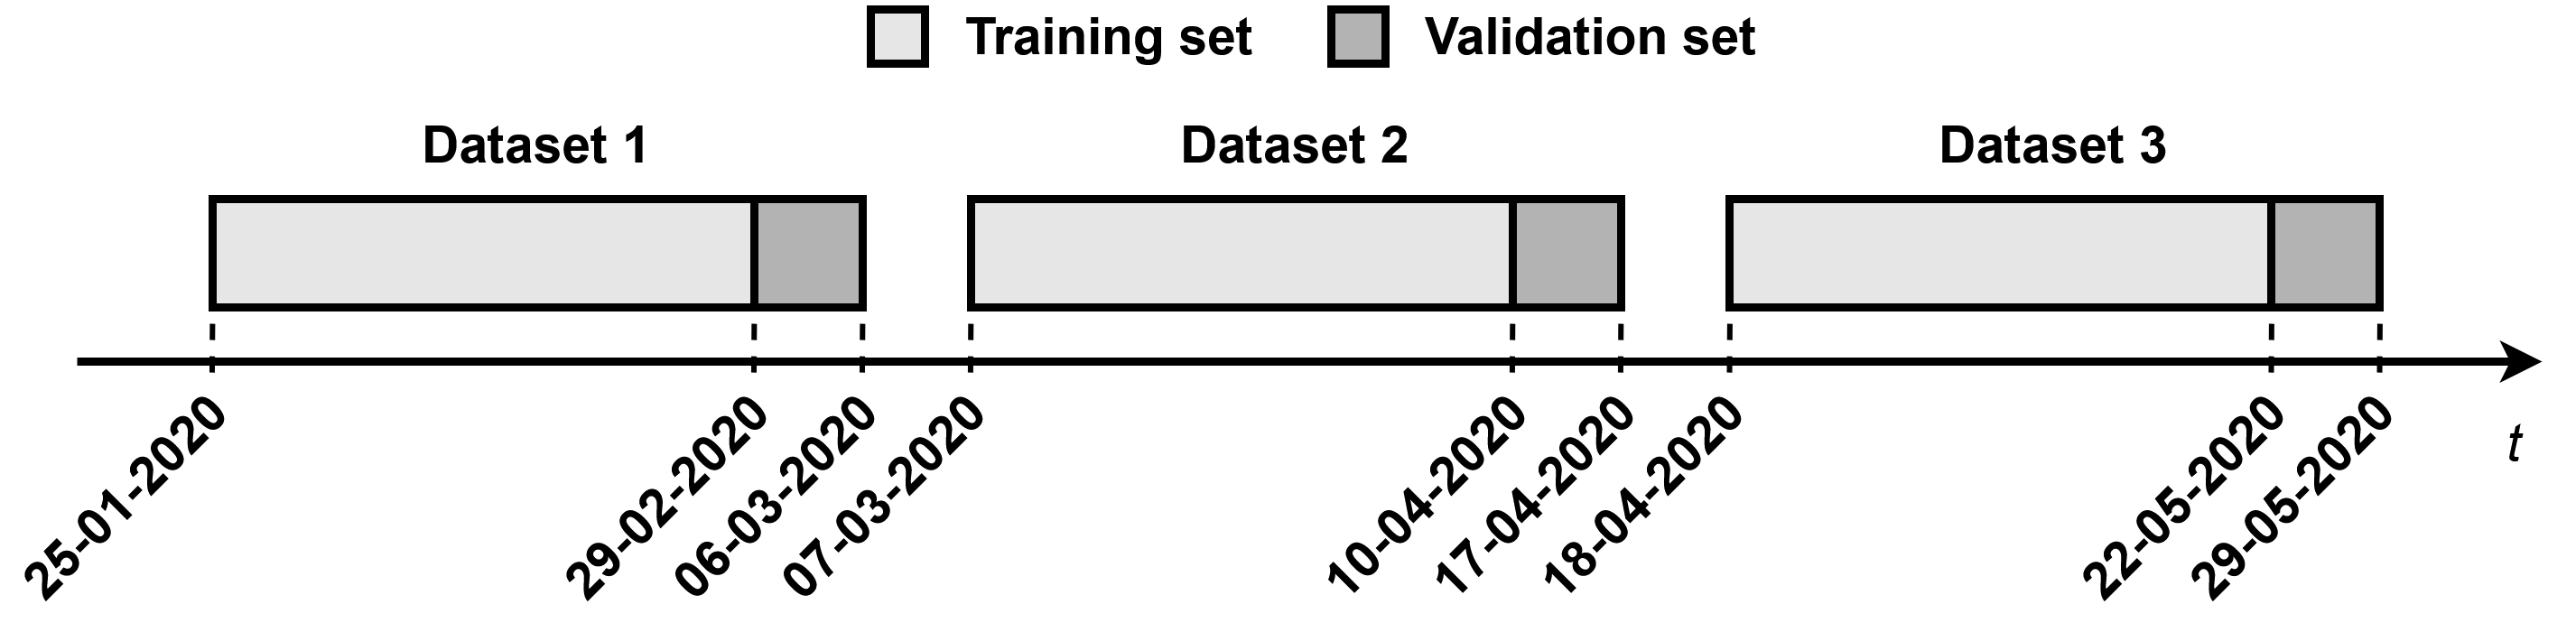
\includegraphics[width=1\textwidth]{Images/hyptun.png}
    \caption{Datasets used for expanding window cross-validation.}
    \label{hyptun}
    \end{center}
\end{figure}

The process of tuning hyperparameters is a long and time consuming process. Although the meaning of each hyperparameter and what it represents in the context of the layer is known, there is no rule dictating which hyperparamters are best for each case. It is an experimental process in which the models must be trained, and validated. The results obtained in the validation data are then compared for different hyperparameter combinations. The combination that presents the best results for each model, must be the one selected. 


Model 1 consists of a input layer, a \ac{GRU} layer, and a dense layer for the output with 3 units, one for each forecast ((t+5), (t+10) and (t+15)). In \ac{GRU} layers, the hyperparameter that can be changed is the number of Units - A positive integer that represents the dimensionality of the output space. This hyperparameter must be tuned in to find a value for which the system performs well. However, the increase of this value represents an increase in the complexity of the model, which makes it slower. In this sense, one tested initially a \ac{GRU} layer with 8 units, then 16 units and later a \ac{GRU} with 32 units. In order to avoid overfitting, a dropout layer with $p$=0.2 to the \ac{GRU} layer output.

Regarding model 2, the structure is relatively similar to model 1 with the difference that it has an \ac{LSTM} layer instead. As in the previous case, it was tested which number of units should be used in the layer, 8 units, 16 units or 32 units. The remaining structure used is similar to model 1.

Models 3 and 4 are similar to models 1 and 2, respectively, with the difference that they are univariates and not multivariates. This means that they have an input feature, Available Power, unlike models 1 and 2, which besides Available Power, also have the remaining features resulting from the \ac{PCA} process.

In models 5 and 6, regarding the \ac{1D CNN} layer, some experiments dictated that a good number of filters - An integer that represents dimensionality of the output space (i.e. the number of output filters in the convolution), to be used could be 8, that is, 8 convolutions are performed that produce the 8 outputs of this layer, but 32 was also tested. The kernel\_size - An integer or tuple/list of a single integer, specifying the length of the 1D convolution window used was 5 units, which means that the output of this layer consists of the result of consecutive convolutions of 5 values, but it was also tested to use a kernel of dimension 10, i.e. convolutions of 10 time-steps. In the Max pooling layer, a pool\_size of 10 units was used, which means that only the highest value every 10 values is taken into account, as explained in the section \ref{chap3:subsubsec:1dcnn}. 


For each of the three blocks defined in the expanding window cross-validation process, the architectures were trained and validated. The hyperarameters already mentioned were progressively optimized in the three blocks, for each model. In Table \ref{tab:layouts}, a summary of the final layouts resulting from the validation process can be found.

% Table generated by Excel2LaTeX from sheet 'Sheet6'
\begin{table}[htbp]
  \centering
  \caption{Models layout with tuned hyperparameters}
    \begin{tabular}{ccc}
    \toprule
    \textbf{Model 1} & \textbf{Model 2} & \textbf{Model 3} \\
    \midrule
    Input (1) & Input (1) & Input (13) \\
    GRU (8) & LSTM (8) & GRU (8) \\
    Dropout (0.2) & Dropout (0.2) & Dropout (0.2) \\
    Dense (3) & Dense (3) & Dense (3) \\
    \midrule
    \textbf{Model 4} & \textbf{Model 5} & \textbf{Model 6} \\
    \midrule
    Input (13) & Input (13) & Input (13) \\
    LSTM (8) & 2 * Conv1D (8, 10) & 2 * Conv1D (8, 10) \\
    Dropout (0.2) & Maxpooling(10) & Maxpooling(10) \\
    Dense (3) & GRU (8) & LSTM (8) \\
      & Dropout (0.2) & Dropout (0.2) \\
      & Dense (3) & Dense (3) \\
    \end{tabular}%
  \label{tab:layouts}%
\end{table}%


Of all the hyperparameter combinations tested, the models referred to in Table \ref{tab:layouts}, were those that presented the best performance in the expanding window cross-validation process, and were therefore considered the final combinations of hyperparameters used in this study. The Table \ref{tab:characteristics} details the number of inputs, hidden layers, hidden nodes and outputs of each model. 


% Table generated by Excel2LaTeX from sheet 'Sheet6'
\begin{table}[htbp]
  \centering
  \caption{Hyperparameters of the final models}
    \begin{tabular}{r|cccccc}
    \toprule
    \multicolumn{1}{c|}{\textbf{Model}} & \textbf{1} & \textbf{2} & \textbf{3} & \textbf{4} & \textbf{5} & \textbf{6} \\
    \midrule
    \# inputs & 13 & 13 & 1 & 1 & 1 & 1 \\
    \# hidden layers & 2-2 & 2-2 & 6-6 & 6-6 & 6-7 & 6-8 \\
    \# hidden nodes &   &   &   &   &   &  \\
    \# outputs & 3 & 3 & 3 & 3 & 4 & 5 \\
    \end{tabular}%
  \label{tab:characteristics}%
\end{table}%


In Table \ref{valres}, the reader may consult the results of the expanding window cross-validation process, which consists of an average of the errors presented in blocks 1, 2 and 3.

\begin{table}[htbp]
  \centering
  \caption{Stage 1 - Expanding window cross-validation results}
       \begin{tabular}{r|cccccccc}
    \toprule
    \multicolumn{1}{c}{} & 0     & 1     & 2     & 3     & 4     & 5     & 6     & 7 \\
    \midrule
    \multicolumn{1}{l|}{\textbf{Non normalized data}} &       &       &       &       &       &       &       &  \\
    \multicolumn{1}{l|}{\textbf{            Validation Score (t+5)      }} &       &       &       &       &       &       &       &  \\
    MSE (E+09)   & \textbf{0.82} & 0.87  & \textbf{0.58} & \textbf{0.67} & 0.90  & 1.18  & 0.91  & 1.02 \\
    RMSE (E+04)   & \textbf{2.84} & 2.92  & \textbf{2.40} & \textbf{2.58} & 2.99  & 3.40  & 2.97  & 3.16 \\
    MAE (E+04)   & \textbf{2.20} & 2.25  & \textbf{1.86} & \textbf{2.06} & 2.30  & 2.62  & 2.30  & 2.45 \\
    \multicolumn{1}{l|}{\textbf{            Validation Score (t+10)               }} &       &       &       &       &       &       &       &  \\
    MSE (E+09)   & \textbf{1.11} & 1.17  & \textbf{0.98} & \textbf{0.99} & 1.20  & 1.42  & 1.16  & 1.28 \\
    RMSE (E+04)   & \textbf{3.30} & 3.39  & \textbf{3.11} & \textbf{3.12} & 3.44  & 3.74  & 3.37  & 3.54 \\
    MAE (E+04)   & \textbf{2.54} & 2.63  & \textbf{2.37} & \textbf{2.43} & 2.65  & 2.89  & 2.59  & 2.76 \\
    \multicolumn{1}{l|}{\textbf{            Validation Score (t+15)               }} &       &       &       &       &       &       &       &  \\
    MSE (E+09)   & \textbf{1.31} & 1.38  & \textbf{1.25} & \textbf{1.24} & 1.43  & 1.63  & 1.38  & 1.51 \\
    RMSE (E+04)   & \textbf{3.58} & 3.68  & \textbf{3.51} & \textbf{3.50} & 3.76  & 4.01  & 3.68  & 3.85 \\
    MAE (E+04)   & \textbf{2.76} & 2.83  & \textbf{2.70} & \textbf{2.71} & 2.89  & 3.09  & 2.82  & 3.01 \\
    \midrule
    \multicolumn{1}{l|}{\textbf{Normalized data}} &       &       &       &       &       &       &       &  \\
    \textbf{Total Validation Score         } &       &       &       &       &       &       &       &  \\
    MSE (E-03)   & \textbf{2.28} & 2.43  & \textbf{2.00} & \textbf{2.11} & 2.47  & 3.03  & 2.36  & 2.56 \\
    RMSE (E-02)   & \textbf{4.70} & 4.84  & \textbf{4.39} & \textbf{4.51} & 4.91  & 5.44  & 4.80  & 5.03 \\
    MAE (E-02)   & \textbf{3.61} & 3.73  & \textbf{3.37} & \textbf{3.51} & 3.77  & 4.20  & 3.69  & 3.90 \\
    \end{tabular}%
  \label{valres}%
\end{table}%



The Table presents the validation \ac{MSE}, \ac{RMSE} and \ac{MAE} for each one of the models, both for the individual forecast for power available in 5, 10 and 15 minutes.



(COMENTÁRIOS AOS DADOS)

\section{Stage 2 - Results}\label{chap3:section:stage_2}

\section{Stage 3 - Discussion}\label{chap3:section:stage_3}
% If Printing on DOUBLE SIDED pages, the second page should be white.
% Otherwise, comment the following command:
\cleardoublepage
%
%Chapter 5
% #############################################################################
% This is Chapter 5
% !TEX root = ../main.tex
% #############################################################################
% Change the Name of the Chapter i the following line
\fancychapter{Forecasting model selection}
\cleardoublepage
% The following line allows to ref this chapter
\label{chap:implementation}

In the past chapters we introduced the theme \ref{chap:intro}, we presented some studies developed in this area \ref{chap:background}, we presented the concrete case studied in this thesis and we proposed a schematization of the work to be developed \ref{chap:architecture}, and we introduced the models that we will implement in this thesis \ref{chap:Model}.
In this chapter, we will present the environment in which the proposed models were trained, the data used and the way how they were treated and used during the research phase, and finally the metrics used to evaluate the performance of the proposed models.
 

\section{Implementation environment} \label{chap5:enviromnet}

During the development of the thesis, several scripts were implemented, both for data processing and for the implementation of machine learning models. The language chosen for this purpose was \textit{Pyhton}. The primary reasons for this choice were the ease of syntax of this language, as well as the large number of libraries available, including \textit{keras}, a Deep Learning library that provides all the necessary tools for building and deploying Neural Networks.

Regarding the hardware components used, two different systems were used during the development of this work. The first environment consists of a CPU (Intel Core i5-3470 3.20GHz), and a GPU (NVIDIA GeForce GTX 1050 Ti) essential to accelerate the training process of the proposed models. The second environment consists of a virtual environment implemented on \textit{Microsoft Azure Machine Learning} platform, where a cluster consisting of a 6 core processor, and a GPU (NVIDIA Tesla K80).

The first environment was used with the purpose of testing, in a first phase, several models with simple tasks, and the second environment was used to put into practice more complex tests that required more computational capacity.
	

\section{Dataset}\label{chap5:dataset}

In this section, we describe the datasets used in the development of this work, and also detail the data preprocessing applied to the datasets so that they had the necessary formatting to be used during this experiment.

\subsection{Data description}

In the day to day of a building, there are many factors that influence its consumption and consequently the available power. In Chapter \ref{chap:background} some examples of work developed with the objective of predicting the energy consumption of a building were mentioned. In Appendix B, Table \ref{table1}, it is possible to verify that generally, two categories of data are used in this kind of applications, data that concern the behavior of the building, and climatic data that characterize the environment in which the building is located.

With respect to data on the behaviour of the building, \ac{EDP} provided two different datasets that present information between January 25, 2020 and September 30, 2020, totalling roughly 8 months of data, with a granularity of 5 seconds. The first dataset includes historical data regarding the energy consumption of the building, and the second dataset includes historical data regarding the solar production generated by the \ac{PV} panels present in the upper part of the building. It is also relevant to mention that the production data provided showed some gaps resulting from sensor reading failures. This aspect implies the need for some mechanisms to complete the missing data.

Regarding climate data, \ac{FCUL} provided two different datasets that present information between January 25, 2020 and June 15, 2020, totaling more or less 5 months of data, with a granularity of 1 minute. The first dataset includes meteorological data regarding the geographical location of the building, and the second includes data regarding solar radiation exerted on the geographical area of the building. Neither of the two datasets had flaws.

In Table \ref{table2}, there is a summary of some key factors regarding the available datasets.


\begin{longtable}{|l|c|c|c|c|}
    \caption{Summary of the datasets used.}
    \label{table2}\\
    
    \hline & \multicolumn{2}{c|}{}&\multicolumn{2}{c|}{}\\[-0.5ex]
    \textbf{Dataset Provider}   & \multicolumn{2}{c|}{\textbf{EDP}} & \multicolumn{2}{c|}{\textbf{FCUL}}\\[1ex]
    \hline & \multicolumn{2}{c|}{}&\multicolumn{2}{c|}{}\\[-0.5ex]

    
    \textbf{Dataset} & \multicolumn{1}{l|}{\textbf{Consumption}} & \textbf{Production} & \multicolumn{1}{l|}{\textbf{Meteorological}} & \textbf{Radiation}  \\
    \textbf{Nº of variables} & \multicolumn{1}{c|}{8} & \multicolumn{1}{c|}{7} &  22  & \multicolumn{1}{c|}{28} \\
    \textbf{Preiod} & \multicolumn{2}{c|}{8 months and 5 days} & \multicolumn{2}{c|}{4 months and 21 days}  \\
    \multicolumn{1}{|r|}{Begin} & \multicolumn{2}{c|}{25-01-2020} & \multicolumn{2}{c|}{25-01-2020} \\
    \multicolumn{1}{|r|}{End}  & \multicolumn{2}{c|}{30-09-2020}  & \multicolumn{2}{c|}{15-06-2020} \\
    \textbf{Nº of days}       & \multicolumn{2}{c|}{249}     & \multicolumn{2}{c|}{142}    \\             
    \textbf{Nº of samples}    & \multicolumn{2}{c|}{4302720} & \multicolumn{2}{c|}{2453760} \\[1ex]
    \hline
    

\end{longtable}

As can be seen through the analysis of Table \ref{table2}, the data provided do not portray the same time window nor have the same granularity. It is then necessary to proceed to some data treatment in order to obtain the data in the desired form.

\subsection{Data manipulation}\label{sec:data_manip}

The data manipulation consists of a process in which the data made available is formatted in such a way that it meets the essential criteria to enable its introduction in the models. During the development of the thesis, this was the most time consuming process. The data treatment is an extremely demanding process, which is simplified in the diagram of Figure \ref{datatreatment}.

\begin{figure}[h!]
    \centering
    \begin{center}
    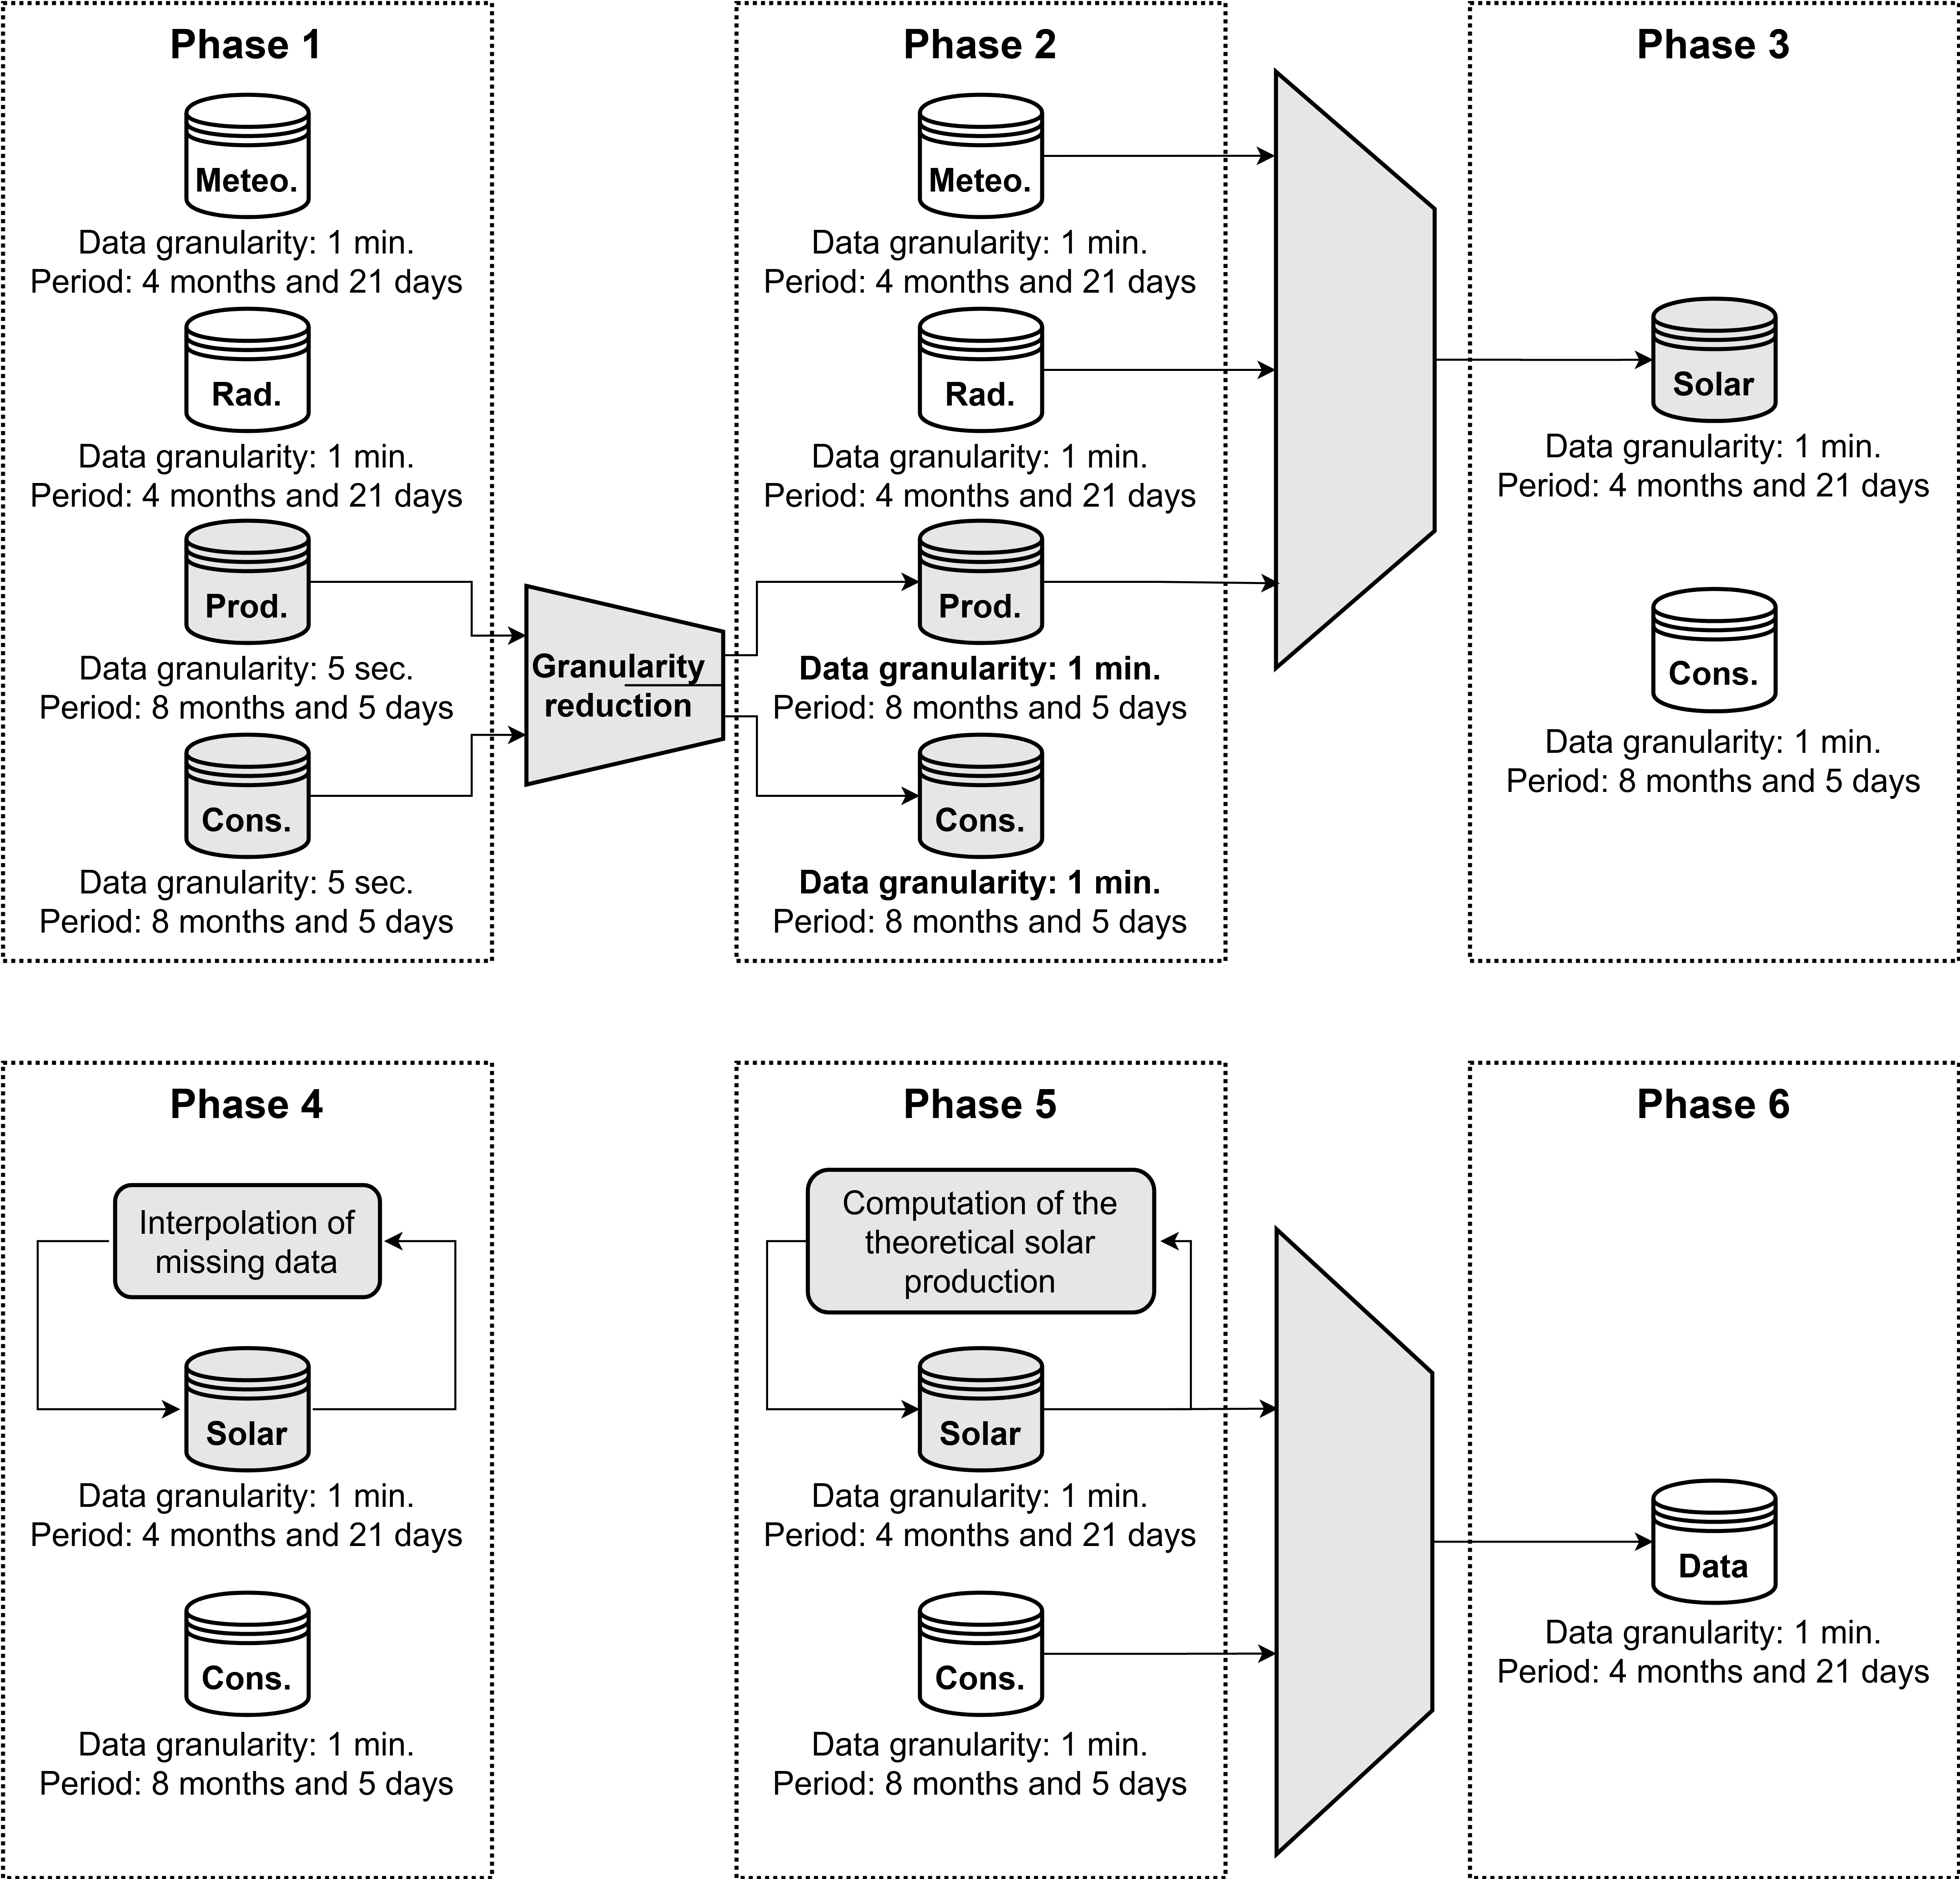
\includegraphics[width=1\textwidth]{Images/Data.png}
    \caption{Data treatment process.}
    \label{datatreatment}
    \end{center}
\end{figure}

In phase 1, the production data (Prod.) is incomplete due to failure of the system responsible for acquiring and storing this indicator. There is also a difference both in granularity and period available, between the data provided by \ac{EDP} and the data provided by \ac{FCUL}. It is then necessary, first of all, to equal the granularity of all four datasets. In order to do that, a function was applied to reduce the granularity of the production (Prod.) and consumption (Cons.) datasets, forcing the frequency of both datasets to one minute. the  The function applies an arithmetic mean given by 

\begin{equation}
     A={\frac {1}{n}}\sum _{i=1}^{n}a_{i}={\frac {a_{1}+a_{2}+\cdots +a_{n}}{n}},
\label{amean}
\end{equation}

where $A$ represents the value of the final measure with frequency of 1 minute, and $n$ represents the number of nodes between that minute range that will be converted to a single value. We then reached phase 2, where the four datasets have the same granularity. Then, the datasets corresponding to the meteorological data (Meteo.), radiation data (Rad.) and production data (Prod.) are concatenated. As a result of this process (phase 3), the dataset (Solar) is formed, which aggregates all the information regarding climate data and solar production data over a period of 4 months and 21 days. The reason behind this phenomenon is that all the production days for which there is no direct correspondence in the meteorological data (Meteo.) and radiation data (Rad.) datasets are rejected. 

As mentioned before, the data regarding the solar production (Prod.) presented some temporal flaws. In order to solve the problem, two solutions were found. For time gaps of less than 30 minutes (phase 4), a quadratic interpolation was applied. As an example, given any three points $(x_0, f(x_0))$, $(x_1, f(x_1))$ and $(x_2, f(x_2))$, the polynomial that interpolates the three points is given by

\begin{equation}
\begin{split}
     & f_2(x)=b_0+b1(x-x_0)+b_2(x-x_0)(x-x1),\\
     & where:\\
     & b_0=f(x_0),\\
     & b_1=f[x_0,x_1]=\frac{f(x_1)-f(x_0)}{x_1-x_0},\\
     & b_2=f[x_0,x_1,x_2]=\frac{\frac{f(x_2)-f(x_1)}{x_2-x_1}-\frac{f(x_1)-f(x_0)}{x_1-x_0}}{x_2-x_0}.\\
\end{split}
\label{poly}
\end{equation}

In order to exemplify the evolution of the incomplete dataset construction, in the graph of Figure \ref{int0} we can observe the solar power generated measured by the sensors on February 3, 2020. In red, is the portion of data that were measured, corresponding to the Solar dataset in Phase 3 represented in Figure \ref{datatreatment}. After the interpolation, to the original dataset are added the points represented in blue, which represent measurement failures of less than 30 minutes. At the end of Phase 4, the dataset is then composed of the data points represented in blue plus the points represented in red.



\begin{figure}[h!]
    \centering
    \begin{center}
    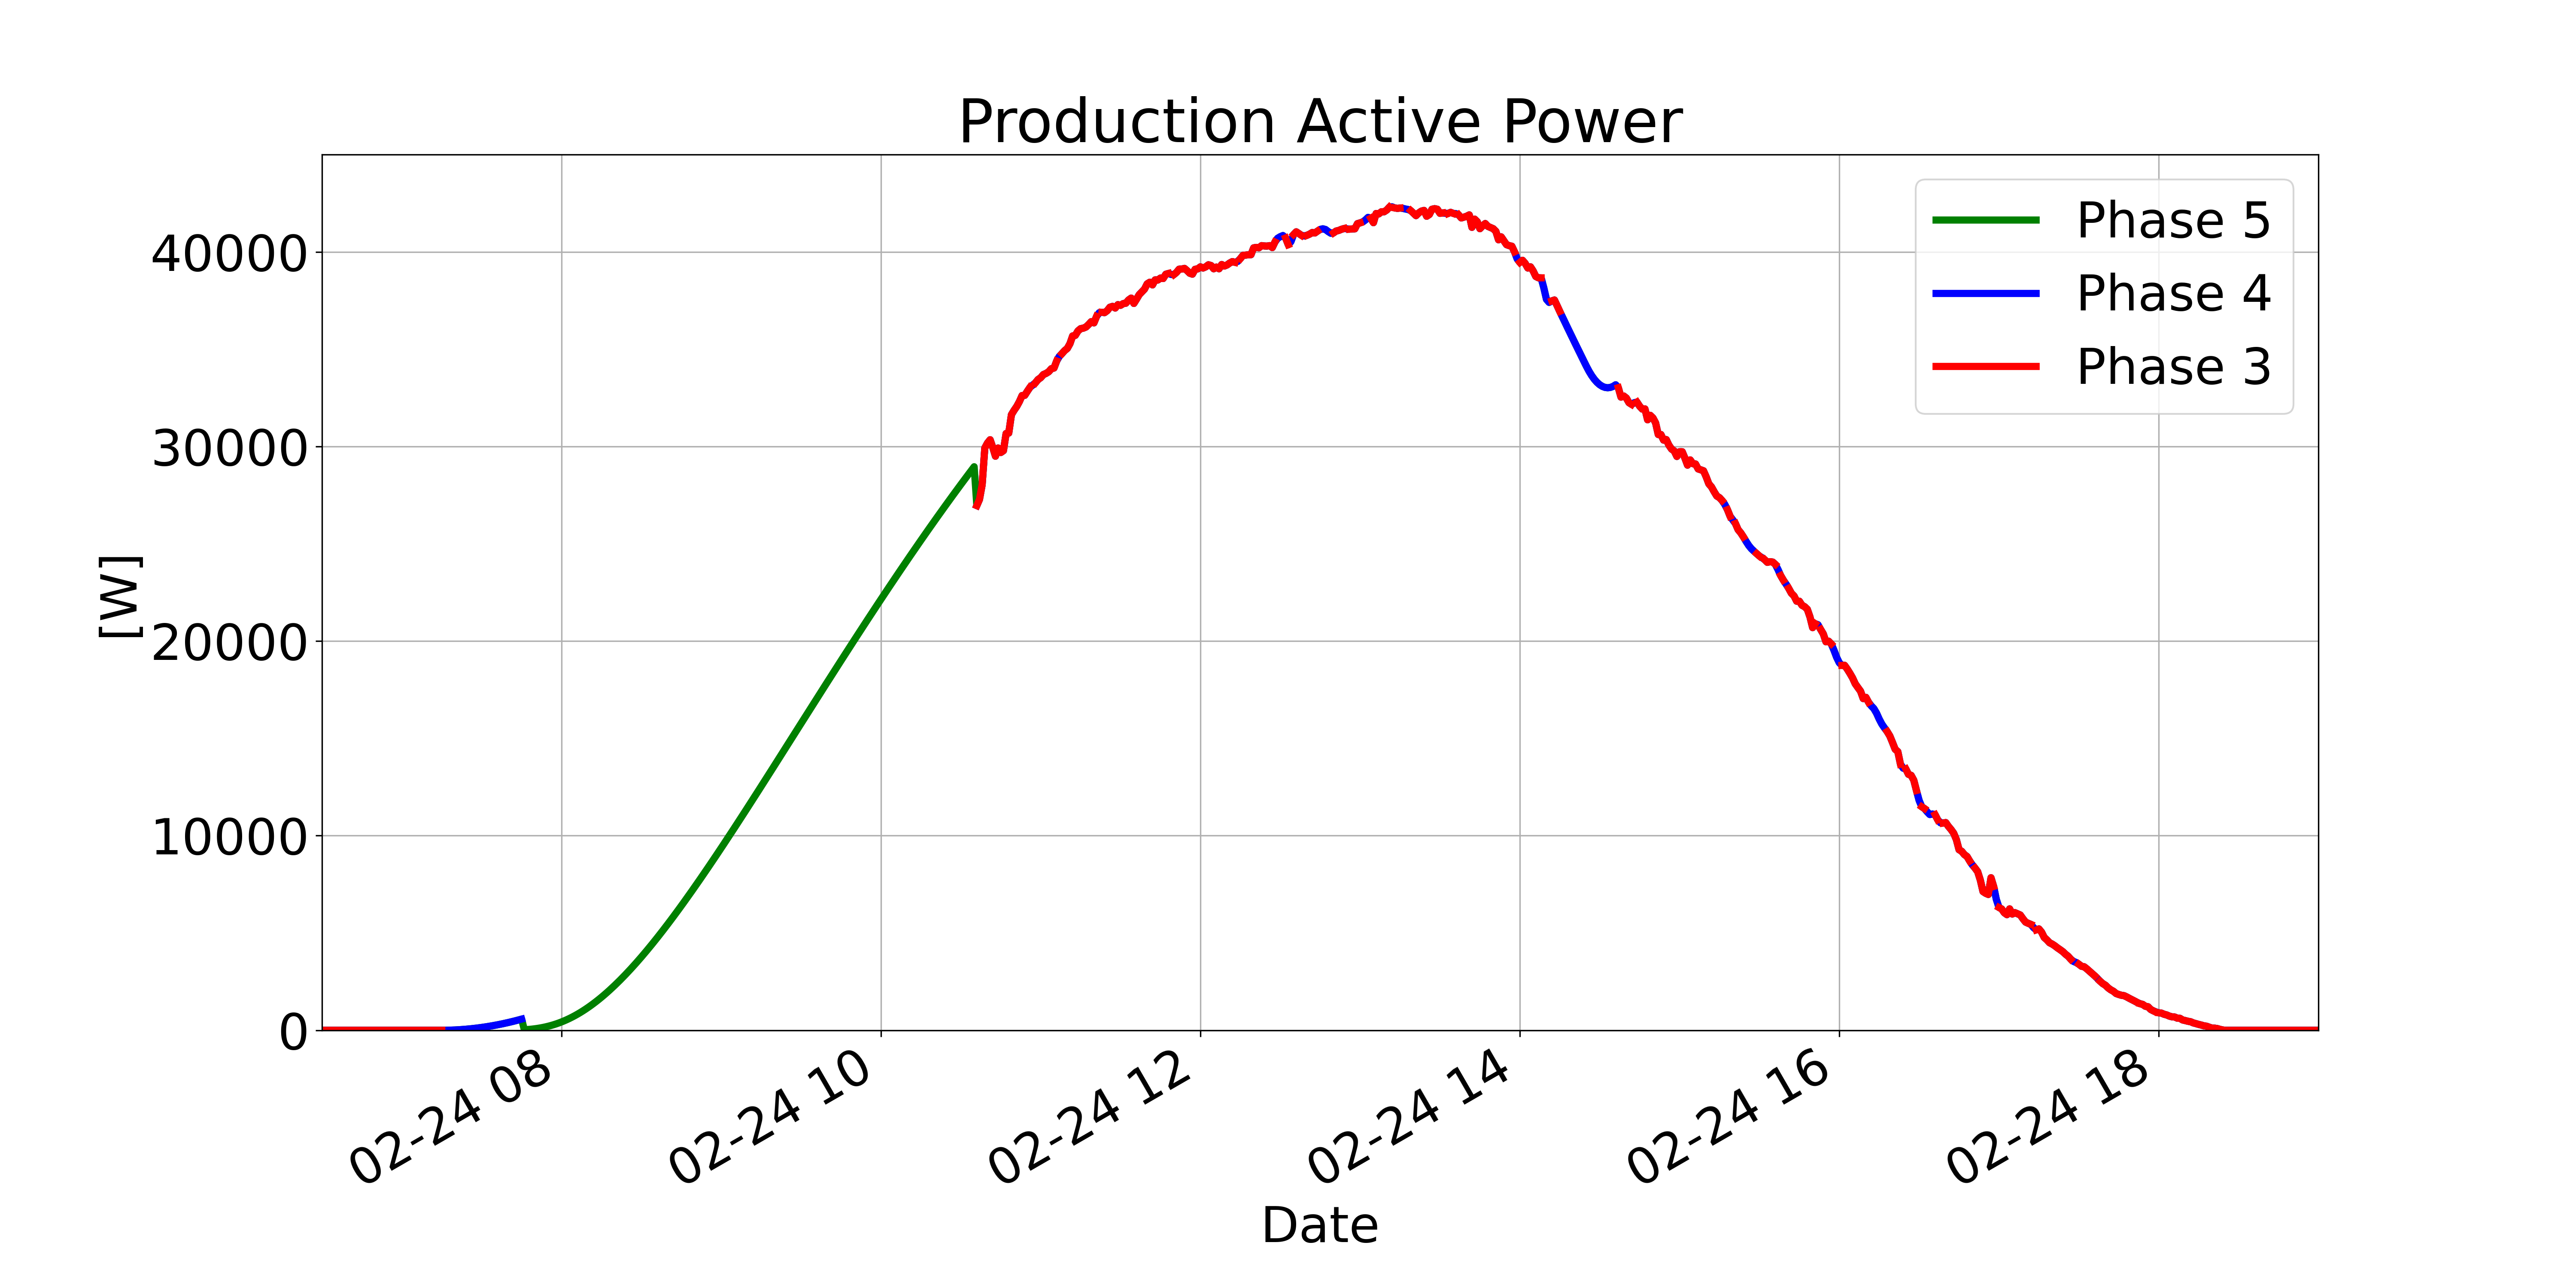
\includegraphics[width=1\textwidth]{Images/int0.png}
    \caption{Data treatment process.}
    \label{int0}
    \end{center}
\end{figure}





For time failures of more than 30 minutes, the dataset was completed with theoretically computed values, since the interpolation for large temporal failures does not present the expected behavior.
Based on the equation of the sun's position in the sky throughout the year, the maximum amount of solar insolation on a surface at a particular tilt angle can be calculated as a function of latitude and day of the year\cite{solar0}. In order to determine the direct component of solar radiation in $kW/m^2$, we used


\begin{equation}
     I_D = I_0*0.7^{(AM^{0.678})}
\label{solar}
\end{equation}

where $I_0$ is the solar intensity external to the Earth's atmosphere that is approximately $1.353 kW/m^2$, $0.7$ represents the overall attenuation of the atmosphere, $AM = \frac{1}{cos\theta}$ is the airmass and $\theta$ is the zenith angle (90° minus the altitude) of the sun. This formula produces an optimal result when there are no clouds. Multiplying the resulting value by the total area of panels in the building and taking into account their positioning efficiency, a theoretical value of power generated by the \ac{PV} panels is obtained, in an ideal scenario. In Phase 5, all missing readings were replaced by the calculated theoretical value, as can be seen in Figure \ref{int0} in green. This way, the Solar dataset was completed. It is possible to verify that the point of change between the theoretical data (the green one) and the original data (the red one) is somewhat sudden, because the green signal considers an ideal scenario and the red signal represents real measurements (affected by clouds, cranes, etc.) The sum of the green, blue and red signals, result in a complete signal for the solar active power generated by the \ac{PV} panels.


In Phase 6 the Solar and Cons. datasets were concatenated, thus reducing the dataset time interval to a final result of 4 months and 21 days.



\subsection{Feature selection}

Although a huge amount of data was made available for the development of this study, the use of a large number of different features may negatively affect the performance of the tested models, namely their speed. In order not to overload the models, an initial set of features from all the available datasets was selected. In Table \ref{table3} the reader may find the selected features, their unit and their descrption.


\begin{longtable}{|l|c|l|}
    \caption{Features used.}
    \label{table3}\\
    
    \hline 
    & &\\[-0.5ex]
    \textbf{Feature}   & \textbf{Unit} & \textbf{Description}\\[1ex]
    \hline
     & &\\[-0.5ex]
    \textbf{$Std\_DHI$} & $W/m^2$ & Standard diffuse horizontal irradiance\\
    \textbf{$Avg\_DHI$} & $W/m^2$ & Average diffuse horizontal irradiance \\
    \textbf{$Avg\_GHI$} & $W/m^2$ & Global horizontal irradiance \\
    \textbf{$Avg\_DNI$} & $W/m^2$ & Direct normal irradiance \\
    \textbf{$Avg\_POA$} & $W/m^2$ & Average plane of array\\
    \textbf{$T\_amb\_avg$} & $^\circ C$ & Average ambient temperature\\
    \textbf{$Theoretical Value$} & $W$ & Theoretical production active power generated\\
    \textbf{$ActPwr$} & $W$ & Production active power\\
    \textbf{$Ir$} & $A$ & Consumption three-phase current \\
    \textbf{$Is$} & $A$ & Consumption three-phase current \\
    \textbf{$It$} & $A$ & Consumption three-phase current \\
    \textbf{$Vrs$} & $V$ & Consumption three-phase voltage\\
    \textbf{$Vst$} & $V$ & Consumption three-phase voltage\\
    \textbf{$Vtr$} & $V$ & Consumption three-phase voltage\\
    \textbf{$P$} & $W$ & Consumption real power\\
    \textbf{$S$} & $VA$ & Consumption complex power\\
    \textbf{$hour$} & $hours$ & Hour of the day\\
    \textbf{$day\_of\_month$} & $days$ & Day of the month\\
    \textbf{$day\_of\_week$} & $days$ & Day of the week\\
    \textbf{$month$} & $months$ & Month of the year\\
    \textbf{$holiday$} & $binary$ & National holiday identifier\\[+1ex]
    \hline
    

\end{longtable}

Although all these features contribute in some way to enrich the past information available, it is important to reduce as much as possible the number of features used as input to the model, limiting the choice to the essentials.
In this sense, a second phase of analysis was then carried out where the correlation matrix between each of the features was projected. In Figure \ref{corr} one can then observe the correlation matrix where the correlations between all the selected variables are represented. The value of the correlation is present in the [-1, 1] range, where -1 means that the variables present an opposite correlation, 0 means that there is no correlation between the two variables and 1 means that there is perfect correlation between the two variables. 


\begin{figure}[h!]
    \centering
    \begin{center}
    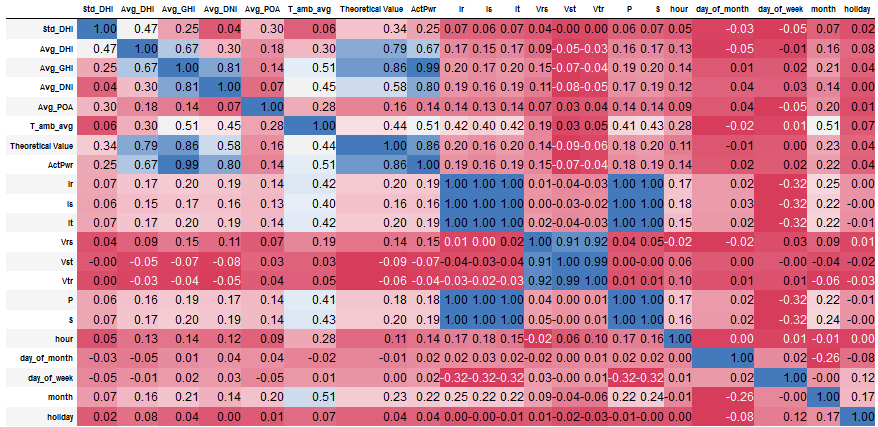
\includegraphics[width=1\textwidth]{Images/corr.PNG}
    \caption{Feature correlation matrix.}
    \label{corr}
    \end{center}
\end{figure}


The aim of computing this matrix is to identify variables that present a perfect or almost perfect correlation between them, in order to eliminate redundancies. 

A perfect correlation between two variables means that one can be deduced from the other, that is, the relevance of the two variables for the construction of the forecasting system is the same, so one of the variables can be eliminated. 


First of all, it was decided to eliminate the features that contribute to the calculation of others. In this sense, both three-phase voltages and three-phase currents contribute to the calculation of $S$ and $P$ and present a perfect correlation between them. It was then chosen to eliminate the features: $Ir$, $Is$, $It$, $Vrs$, $Vst$, $Vtr$. Then, since in this case $S$ does not have an imaginary component, $S$ and $P$ have the same value. The feature $S$ was then also eliminated. Also, although $Theoretical\ Value$ and $Avg\_GHI$ present a very high correlation with $ActPwr$ (which is predictable given that the measured $ActPwr$ these two variables were added, as explained in section X), we chose to keep these two variables as input features since the correlation is not exactly perfect and can be decisive in certain cases in building a good predictive model. Therefore, the variables chosen for the input of all tested models are: $Std\_DHI$, $Avg\_DHI$, $Avg\_GHI$, $Avg\_DNI$, $Avg\_POA$, $T\_amb\_avg$, $Theoretical\ Value$, $ActPwr$, $P$, $hour$, $day\_of\_month$, $day\_of\_week$, $month$ and $holiday$. In addition, the variable $Available Powe$ given in $watts$ has been added as an input feature, resulting in a total of 15 input features and 1 output.



SLIDING WINDOWXXXXXX

\subsection{Data partition}\label{sec:datap}

In order to study a certain algorithm, it is necessary to have access to past data to train the model and then evaluate its performance. The the available data as well is an important factor when it comes to developing predictive models. Usually, in \ac{ML}, to study a certain model, the dataset should be divided into three sets as can bee seen in Figure \ref{division}. 

\begin{figure}[h!]
    \centering
    \begin{center}
    
\includegraphics[width=1\textwidth]{Images/division.png}
    \caption{Dataset division.}
    \label{division}
    \end{center}
\end{figure}

The first set is known as a training set, and consists of a dataset used to feed the model with examples in order to fit the hyperparameters, such as the weights of connections between neurons in artificial neural networks. As the name implies, the training set is suitable to train the model, progressively adapting the model to its intended purpose. The second is the validation set, which is responsible for simultaneously continuing to adapt the hyperparameters of the model, while providing an unbiased evaluation of the model fit. In addition to that, it can be used for regularization, as is the case of eraly-stopping, referred to in section \ref{sec:early}. Finally, the test set is an independent dataset of the two previous ones, which has as main objective to evaluate in an unbiased way the performance of the model in unseen data (data that was not used neither in the training process nor in the validation process). 

In this study, a distribution with 80\% of training data, 10\% of validation data and 10\% of test data was used. Other combinations were tested as 90\% - 5\% - 5\% and 70\% - 15\% - 15\%, but always obtained poorer results. 

One way to use the available dataset to evaluate the proposed models would be to simply apply the standard training-validation-testing division to the entire dataset available, but this strategy would be a poor way to use the small amount of data available. Typically, to evaluate machine learning models on a very limited time interval, k-fold cross-validation is used. However, cross-validation can present some problems when applied to time-series problems, since one cannot choose random samples and assign them to either the test set or the training set because it makes no sense to use future values to predict past values. There is a time dependency between observations, and it is essential to preserve this relationship during testing. To overcome this barrier, a block cross-validation method was used.

In Figure \ref{partition} the reader may find four different sub-datasets, resulting from a division of the main datastet, defined in phase 6, of the section \ref{sec:data_manip}. The idea behind this division is, in a first part, to use datasets 1, 2 and 3 for training and validation in order to make hyperparameter tuning, and use dataset 4 to test the final models.

\begin{figure}[h!]
    \centering
    \begin{center}
    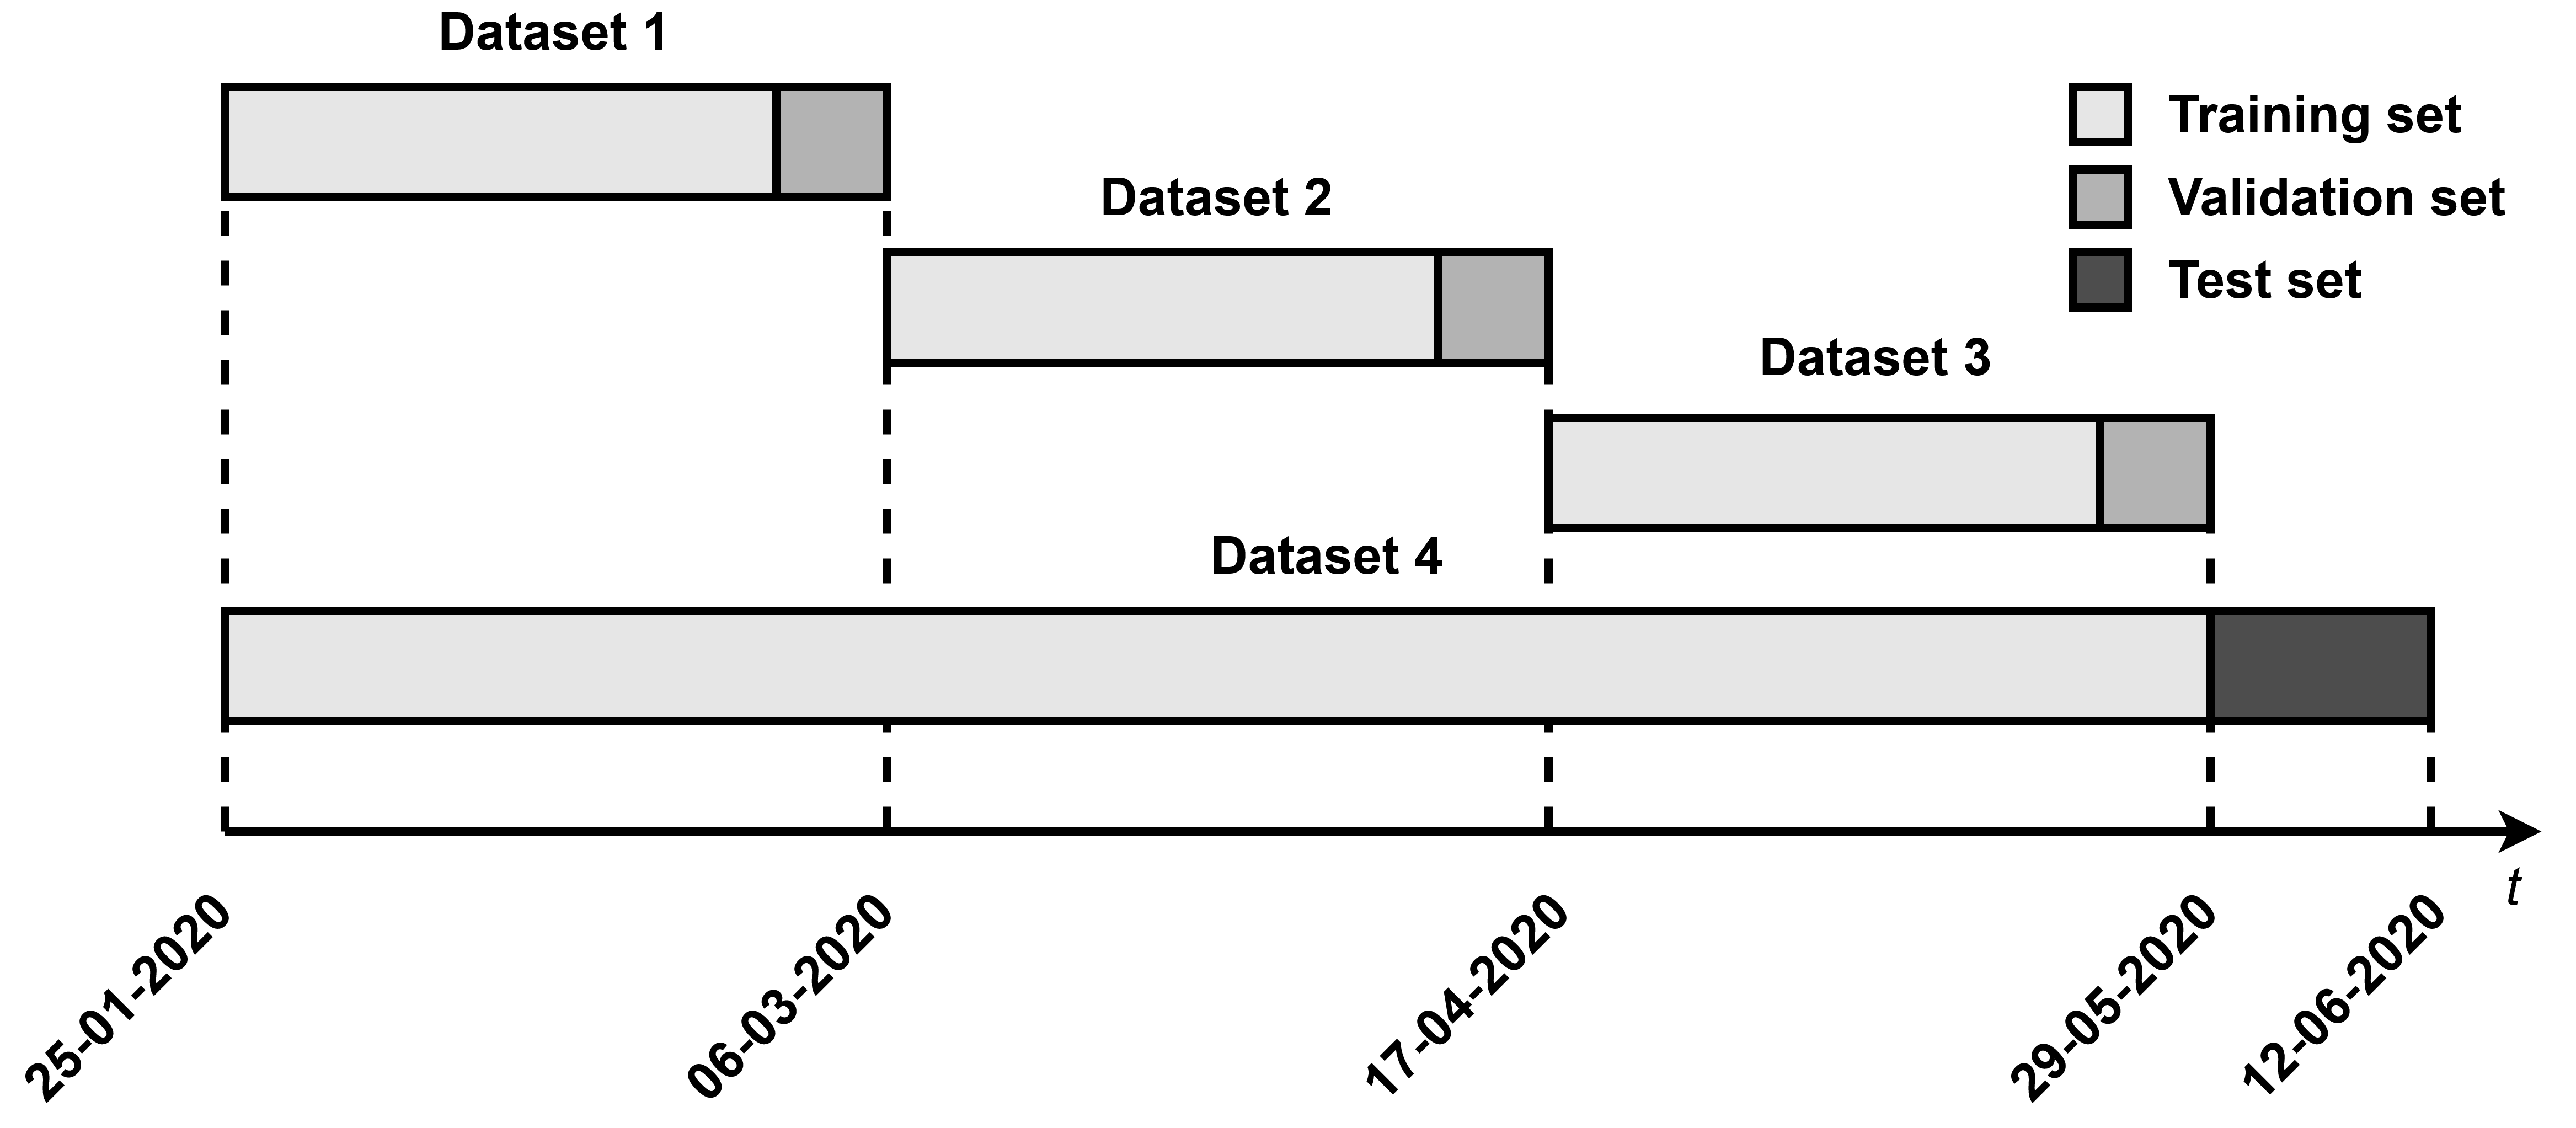
\includegraphics[width=1\textwidth]{Images/data_partition.png}
    \caption{Data partition diagram.}
    \label{partition}
    \end{center}
\end{figure}

Datesets 1, 2 and 3 feature five weeks of training and one week of validation. The dataset 4, however, presents 18 weeks of training and two tests. The overall goal is to propose a model capable of predicting the available power between May 25 and June 12. The standard approach would be to split dataset 4 in training, validation and testing.  Block cross-validation consists of dividing the training set in a fixed number of blocks, and perform training and validation on these blocks. The overall performance evaluation of the models is then given by the average of the performance in each of these blocks i.e., the error of the models is given by

\begin{equation}
     Model\ error =\frac {1}{k}\ \sum_{i=1}^k Error_{di},
\label{err_av}
\end{equation}

where $Model\ error$ represents the final model error, and $Error_{di}$ represents the error that the model presented while performing in dataset $i$, and $k$ represents the number of datasets used.
In this specific case, the validation error for each model is given by

\begin{equation}
     Model\ error =\frac {1}{3}\ (Error_{d1} + Error_{d2} + Error_{d3}).
\label{err_av}
\end{equation}

The great advantage of using this method is the reduction of the influence of eventual points in the choice of the best model. In other words, by performing an average of 3 different sets, the robustness of the choice process is increased since different scenarios are considered and the best model is the one that performs well on average for all of them.

\section{Performance evaluation metrics}\label{chap5:evaluation}

In the previous section, important details concerning the data used in this thesis were explained. One defined $Model\ error$, but did not specify which concrete metrics were used in this work. To compare the performance of the different models in the defined dataset, it is necessary to use some measures of forecast performance. In this sense, during this thesis four different measures were used that relate the real values present in the time series represented by $y_t$, and the forecast values, which are represented by $f_t$. Thus, the forecast error is given by $e_t=y_t-f_t$. The three measures presented are quite common in the literature \cite{} and are described below.

\subsection{Mean Absolute Error (MAE)}

The \ac{MAE}, is defined as

\begin{equation}
     MAE =\frac {\sum_{t=1}^n|e_t|}{n}.
\label{mae}
\end{equation}

The \ac{MAE} is known as a scale-dependent accuracy measure and measures the average absolute deviation between the forecasted values and the real ones. As a scale-dependent measure, it cannot be used to compare series series using different scales.


\subsection{Mean Squared Error (MSE)}

The \ac{MSE}, is defined as

\begin{equation}
     MSE =\frac {1}{n}\sum_{t=1}^ne_t^2.
\label{mse}
\end{equation}

The \ac{MSE} is also known as a scale-dependent accuracy measure and measures the average squared deviation between the forecasted values and the real ones. The application of this measure is quite relevant because it doesn't allow the negative errors to cancel the positive errors and vice-versa. 

\subsection{Root Mean Squared Error (RMSE)}

By applying the square root to the \ac{MSE}, the \ac{RMSE} is then defined as

\begin{equation}
     RMSE =\sqrt{MSE} = \sqrt{\frac {1}{n}\sum_{t=1}^ne_t^2}.
\label{rmse}
\end{equation}

The advantage of \ac{RMSE} over \ac{MSE} is that it is on the same scale as the targets, facilitating its interpretation in the concrete context of the problem. 

\section{Algorithm selection} \label{chap5:framework}

In this section, we explain the 8 architectures introduced in the section \ref{sec:arq}, and describe the method used to optimize the hyperparameters of each of the models. In addition, we also choose the models that present the best performance for specific situations such as holidays and weekends. At the end of this section, the goal is to find a model or a set of models that present good overall performance.


\subsection{Part 1 - Hyperparameter tuning}\label{sec:part1}
In the first part of the process, the focus was to optimize the hypterparameters of the 8 proposed architectures in order to obtain the best set of hyperparameters for each of the eight architectures. To do so, a script was developed responsible for training and validating all possible combinations of different hyperparameters (within a predefined range), for each one of the 3 Datasets mentioned in section \ref{sec:datap}. In Table \ref{table4} the different combinations of hyperparameters tested for each of the architectures can be observed.

\begin{longtable}{|c|c|c|c|}
    \caption{Combinations of hyperparameters tested.}
    \label{table4}\\
    \hline 
    & & & \\[-0.5ex]
    \textbf{Model} & \textbf{Architecture}   & \textbf{Hyperparameters tested values} & \makecell*[{{p{2.5cm}}}]{\centering\textbf{Total number of combinations}}\\[3ex]
    \hline
    & & & \\[-2ex]
    Model 0 & GRU & \makecell*[{{p{6.3cm}}}]{\centering Units - [8, 16, 32, 64, 128, 256, 512]} & 7\\
    \hline
    Model 1 & LSTM & \makecell*[{{p{6.3cm}}}]{\centering Units - [8, 16, 32, 64, 128, 256, 512]} & 7\\
    \hline
    Model 2 & 1D CNN - GRU & \makecell*[{{p{6.3cm}}}]{\centering Filters - [8, 16, 32, 64, 128, 256], Kernel\_size - [10,60], \\Units - [8, 16, 32, 64, 128, 256]} & 72\\
    \hline
    Model 3 & 1D CNN - LSTM & \makecell*[{{p{6.3cm}}}]{\centering Filters - [8, 16, 32, 64, 128, 256], Kernel\_size - [10,60], \\Units - [8, 16, 32, 64, 128, 256]} & 72\\
    \hline
    Model 4 & GRU - GRU & \makecell*[{{p{6.3cm}}}]{\centering Units - [8, 16, 32, 64, 128] (2x)} & 25\\
    \hline
    Model 5 & LSTM - LSTM & \makecell*[{{p{6.3cm}}}]{\centering Units - [8, 16, 32, 64, 128] (2x)} & 25\\
    \hline
    Model 6 & GRU - LSTM & \makecell*[{{p{6.3cm}}}]{\centering Units - [8, 16, 32, 64, 128] (2x)} & 25\\
    \hline
    Model 7 & LSTM - GRU & \makecell*[{{p{6.3cm}}}]{\centering Units - [8, 16, 32, 64, 128] (2x)} & 25\\
    \hline
    & & & \\[-0.5ex]
    \textbf{Total} & \textbf{-} &  \textbf{-} & \textbf{258}\\[+1ex]
    \hline
    

\end{longtable}

Models 0, 1, 4, 5, 6 and 7 only consist of \ac{GRU} and/or \ac{LSTM} layers. In this type of layers, the hyperparameter that changed was only the number of Units - A positive integer that represents the dimensionality of the output space. In models 4, 5, 6 and 7, these values are combined 2 to 2 (8-8, 8-16,... 128-64, 128-128), producing 25 different combinations. On Models 2 and 3, the parameters that are varied are the number of filters of the \ac{1D CNN} - An integer that represents dimensionality of the output space (i.e. the number of output filters in the convolution), the kernel\_size of the \ac{1D CNN} - An integer or tuple/list of a single integer, specifying the length of the 1D convolution window used, and again, the number of Units of the \ac{GRU} and \ac{LSTM} layers. With all these variants, 258 different models are then built and put to the test. The function of this first step is to reduce these 258 models to the best 8, thus selecting the best hyperparameters for each of the 8 architectures. It should be mentioned that, although after the treatment carried out in Part 1 the ideal hyperparameters for each of the 8 network structures are obtained, these values should only be used as indicators. If one verifies that the change of a parameter affects positively the model, then this change should be made.


In Appendix C, Table \ref{table7}, 













\subsection{Part 2 - Situational study}

In the second part of the process, the main objective is to compare the 8 models chosen in Part 1, situationally. To bring this into practice, multiple subdasets were created presenting particular situations in the activity of the building such as weekends, holidays, etc.

This step serves to identify which model presents the best performance depending on the situation to be expected. If it is possible to define a model that is clearly better to predict certain situations, and another that presents better performance in others, there is the possibility of creating a superior abstraction layer capable of choosing the best model to use in a given scenario. In Table {} are present the different scenarios tested as well as the number of cases used in choosing the best model for the scenario in question.

\begin{longtable}{|c|c|}
    \caption{Scenarios tested.}
    \label{table5}\\
    \hline 
    & \\[-0.5ex]
    \textbf{Scenario} & {\centering\textbf{Total number of cases}}\\[1ex]
    \hline
    & \\[-0.5ex]
    National holiday & 6\\
    Weekends & X\\
    Rainy days & \\
    Cold days & \\[1ex]
    \hline
    

\end{longtable}

For each of the cases presented in Table \ref{table5}, a dataset was created whose training subset represents the scenario to be tested. In order to understand which of the 8 models presents the best performance for each scenario, the equation \ref{err_av} was used again. Applying a specific case, the best model to apply in a holiday scenario will be the one that presents on average the lowest error value in the 6 scenarios where it was tested.

\subsection{Part 3}

\subsection{Framework diagram}


\section{Conclusion}

In this chapter, we have delved into the whole process of implementing the work of this thesis. Initially, in the section \ref{chap5:enviromnet}, we describe the different implementation environments used, and then, in the section \ref{chap5:dataset}, we describe the datset used and all the data processing that was performed. In the section \ref{chap5:framework}, we present the test framework and the process chosen to select the best models. Finally, in the section \ref{chap5:evaluation}, we describe the metrics used to choose the best models designed.
% If Printing on DOUBLE SIDED pages, the second page should be white.
% Otherwise, comment the following command:
\cleardoublepage
%
%Chapter 6
%% #############################################################################
% This is Chapter 6
% !TEX root = ../main.tex
% #############################################################################
% Change the Name of the Chapter i the following line
\fancychapter{Experimental Work \& Results}
\cleardoublepage
% The following line allows to ref this chapter
\label{chap:results}

So far we have introduced the theme to be developed in this thesis \ref{chap:intro}, we have presented some studies developed in this area \ref{chap:background}, we have presented the concrete case studied in this thesis and we propose a schematization of the work to be developed \ref{chap:architecture}, we have introduced the models that we will implement \ref{chap:Model}, and we have described in detail both the datasets used, as well as the experimental process implemented in this study \ref{chap:implementation}. In this chapter, we present the results obtained in this thesis as well as a discussion section.


\section{Model selection} \label{chap5:framework}

In this section, the process of training and validation of the proposed system begins. In a first stage, the eight architectures of level 1 are trained and validated in order to perform hyperparameter optimization. It is at this stage that the performance of each architecture is evaluated for the training and validation scenario, by performing the block cross-validation procedure. At the end of this stage, the three best models of the eight initially proposed are chosen, and are retrained on the entire dataset 4, used for the block cross-validation, and are tested in a new unseen set of data, dataset 5.

In the second stage, the resulting forecasts of the three models in dataset 5, are used as input for a new model that should compute new forecasts for 5, 10 and 15 minutes. The second phase then consists in developing the level 2 model, trained and validated in dataset 5, where the tuning of its hyperparameters takes place. The total system implemented to test and choose the models, both of level 1 and level 2, is represented in Appendix C, Figure \ref{levels}.

In the third stage, the final results are presented and a comparative analysis is made between the new hybrid ensemble model, and the other simple models.

\subsection{Stage 1 - Level 1 model selection}\label{sec:part1}

The level 1 model selection process, concerns the selection of the three best models, which consists of optimizing the hypterparameters of the eight proposed architectures for level 1, and selecting the best three. To do that, the datasets 1, 2 and 3 represented in Figure \ref{hyptun}, were used, each one consisting of a total of 4 weeks of data, 3 of which were used for training and 1 for validation. The Block cross-validation process described before, is put into practice with these three sets of data, where the eight models are tested and validated in each of the three sets and the errors presented in each of the validation processes are recorded. At the end of this process, an average of the errors presented in each of the three datasets is computed, for the eight architectures, and those presenting the least error are selected. 

\begin{figure}[h!]
    \centering
    \begin{center}
    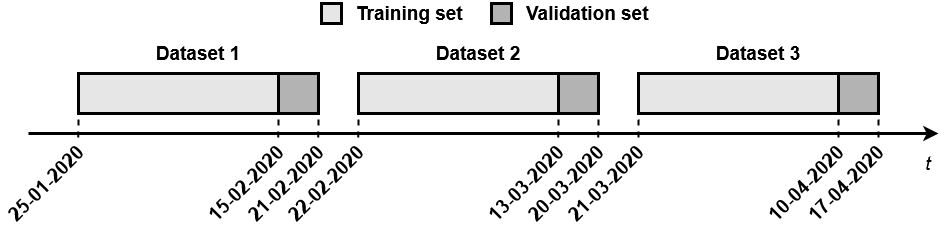
\includegraphics[width=1\textwidth]{Images/hyptun_1.png}
    \caption{Datasets used for training and validation.}
    \label{hyptun}
    \end{center}
\end{figure}

Since the process of tuning the hyperparameters is done by hand, all the architectures started this phase with layers of 8 units. In models 2 and 3 the initial number of filters of the \ac{1D CNN} layers was also 8 and the kernel\_size used was initially 2. If the models behaved well in the validation set and showed no signs of overfitting or underfitting, the initial values would be maintained. If any of these behaviors were observed in at least one of the datasets, the hyperparameters would be changed, or new layers would be added, until the model presented the desired behavior for all the datasets. It was chosen to start with simple architectures and one would only increase the complexity of the architecture (increasing the number of units per layer, for example) if the model did not present all the desired behavior. The increase in the complexity of the model is associated with an increase in its running time, so it was essential to use models as simple as possible. 


Model 0 consists of a input layer with 15 inputs, a \ac{GRU} layer, and a dense layer for the output with 3 units, one for each forecast ((t+5), (t+10) and (t+15)). In \ac{GRU} layers, the hyperparameter that can be changed is the number of Units - A positive integer that represents the dimensionality of the output space. This hyperparameter must be tuned in to find a value for which the system performs well. However, the increase of this value represents an increase in the complexity of the model, which makes it slower.  In this sense, one tested initially a \ac{GRU} layer with 8 units and later a \ac{GRU} with 32 units. Between the two, the structure that presented the best performance was the one with 8 units. In order to avoid overfitting, a drop layer with $p$=0.2 to the \ac{GRU} layer output.

Regarding model 1, the structure is relatively similar to model 0 with the difference that it has an \ac{LSTM} layer instead. As in the previous case, it was tested which number of units should be used in the layer, 8 units or 32 units.  Again, the 8-unit layer showed better performance and was therefore chosen. The remaining structure used is similar to model 0.

Since the layers of 8 units showed a good behavior for models 0 and 1, this variable was not altered anymore for the remaining models. In the remaining six models, \ac{GRU} and \ac{LSTM} layers of 8 units were always used.

In models 2 and 3, regarding the \ac{1D CNN} layer, some experiments dictated that a good number of filters - An integer that represents dimensionality of the output space (i.e. the number of output filters in the convolution), to be used could be 8, that is, 8 convolutions are performed that produce the 8 outputs of this layer, but 32 was also tested. The kernel\_size - An integer or tuple/list of a single integer, specifying the length of the 1D convolution window used was 2 units, which means that the output of this layer consists of the result of consecutive convolutions of 2 values, but it was also tested to use a kernel of dimension 10, i.e. convolutions of 10 time-steps that represent 10 minutes, and also of 60 time-steps, i.e. one hour. In the Max pooling layer, a pool\_size of 10 units was used, which means that only the highest value every 10 values is taken into account, as explained in the section \ref{sec:1dcnn}.

In models 4, 5, 6 and 7, since they since they are composed of multiple \ac{GRU} and/or \ac{LSTM} layers, again layers with only 8 units were used. These four models represent all possible combinations two layers of type \ac{GRU} and \ac{LSTM}. 

In Table \ref{tableModels}, a summary of the final models used in the validation process can be found. Factors such as the proposed structure and the number of parameters used are detailed.

\begin{table}[htbp]
  \centering
  \caption{Model specifications.}
    \begin{tabular}{r|cccccccc}
          & \multicolumn{8}{c}{Level 1 Model} \\
    \midrule
    \textbf{Model} & \multicolumn{2}{c}{0} & \multicolumn{2}{c}{1} & \multicolumn{2}{c}{2} & \multicolumn{2}{c}{3} \\
    \midrule
          & \multicolumn{2}{c}{Input (15)} & \multicolumn{2}{c}{Input (15)} & \multicolumn{2}{c}{Input (15)} & \multicolumn{2}{c}{Input (15)} \\
          & \multicolumn{2}{c}{GRU (8)} & \multicolumn{2}{c}{LSTM (8)} & \multicolumn{2}{c}{Conv1D (8, 2)} & \multicolumn{2}{c}{Conv1D (8, 2)} \\
          & \multicolumn{2}{c}{Dropout (0.2)} & \multicolumn{2}{c}{Dropout (0.2)} & \multicolumn{2}{c}{Maxpooling(10)} & \multicolumn{2}{c}{Maxpooling(10)} \\
          & \multicolumn{2}{c}{Dense (3)} & \multicolumn{2}{c}{Dense (3)} & \multicolumn{2}{c}{GRU (8)} & \multicolumn{2}{c}{LSTM (8)} \\
          & \multicolumn{2}{c}{} & \multicolumn{2}{c}{} & \multicolumn{2}{c}{Dropout (0.2)} & \multicolumn{2}{c}{Dropout (0.2)} \\
          & \multicolumn{2}{c}{} & \multicolumn{2}{c}{} & \multicolumn{2}{c}{Dense (3)} & \multicolumn{2}{c}{Dense (3)} \\
    \midrule
    \textbf{Model} & \multicolumn{2}{c}{4} & \multicolumn{2}{c}{5} & \multicolumn{2}{c}{6} & \multicolumn{2}{c}{7} \\
    \midrule
          & \multicolumn{2}{c}{Input (15)} & \multicolumn{2}{c}{Input (15)} & \multicolumn{2}{c}{Input (15)} & \multicolumn{2}{c}{Input (15)} \\
          & \multicolumn{2}{c}{GRU (8)} & \multicolumn{2}{c}{LSTM (8)} & \multicolumn{2}{c}{GRU (8)} & \multicolumn{2}{c}{LSTM (8)} \\
          & \multicolumn{2}{c}{Dropout (0.2)} & \multicolumn{2}{c}{Dropout (0.2)} & \multicolumn{2}{c}{Dropout (0.2)} & \multicolumn{2}{c}{Dropout (0.2)} \\
          & \multicolumn{2}{c}{GRU (8)} & \multicolumn{2}{c}{LSTM (8)} & \multicolumn{2}{c}{LSTM (8)} & \multicolumn{2}{c}{GRU (8)} \\
          & \multicolumn{2}{c}{Dropout (0.2)} & \multicolumn{2}{c}{Dropout (0.2)} & \multicolumn{2}{c}{Dropout (0.2)} & \multicolumn{2}{c}{Dropout (0.2)} \\
          & \multicolumn{2}{c}{Dense (3)} & \multicolumn{2}{c}{Dense (3)} & \multicolumn{2}{c}{Dense (3)} & \multicolumn{2}{c}{Dense (3)} \\
    \midrule
    \textbf{Model} & 0     & 1     & 2     & 3     & 4     & 5     & 6     & 7 \\
    \midrule
    \# inputs & 15    & 15    & 15    & 15    & 15    & 15    & 15    & 15 \\
    \# hidden layers & 2     & 2     & 4     & 4     & 4     & 4     & 4     & 4 \\
    \# hidden nodes & 16    & 16    & 16    & 16    & 16    & 16    & 16    & 16 \\
    \# outputs & 3     & 3     & 3     & 3     & 3     & 3     & 3     & 3 \\
    \end{tabular}%
  \label{tableModels}%
\end{table}%

After defining the structural details of the models to be evaluated, a block cross-validation process was then carried out where Datasets 1, 2 and 3 were trained and validated with a distribution of 75\% training and 25\% validation, i.e. three weeks training and one week of validation. In Appendix D, Tables \ref{table4}, \ref{table5} and \ref{table6}, the reader can find the results of the errors presented in each one of the three datastes. In Table \ref{valres}, the reader may consult the results of the block cross-validation process, which consists of an average of the errors presented in datasets 1, 2 and 3.

\begin{table}[htbp]
  \centering
  \caption{Stage 1 - Block cross-validation results}
       \begin{tabular}{r|cccccccc}
    \toprule
    \multicolumn{1}{c}{} & 0     & 1     & 2     & 3     & 4     & 5     & 6     & 7 \\
    \midrule
    \multicolumn{1}{l|}{\textbf{Non normalized data}} &       &       &       &       &       &       &       &  \\
    \multicolumn{1}{l|}{\textbf{            Validation Score (t+5)      }} &       &       &       &       &       &       &       &  \\
    MSE (E+09)   & \textbf{0.82} & 0.87  & \textbf{0.58} & \textbf{0.67} & 0.90  & 1.18  & 0.91  & 1.02 \\
    RMSE (E+04)   & \textbf{2.84} & 2.92  & \textbf{2.40} & \textbf{2.58} & 2.99  & 3.40  & 2.97  & 3.16 \\
    MAE (E+04)   & \textbf{2.20} & 2.25  & \textbf{1.86} & \textbf{2.06} & 2.30  & 2.62  & 2.30  & 2.45 \\
    \multicolumn{1}{l|}{\textbf{            Validation Score (t+10)               }} &       &       &       &       &       &       &       &  \\
    MSE (E+09)   & \textbf{1.11} & 1.17  & \textbf{0.98} & \textbf{0.99} & 1.20  & 1.42  & 1.16  & 1.28 \\
    RMSE (E+04)   & \textbf{3.30} & 3.39  & \textbf{3.11} & \textbf{3.12} & 3.44  & 3.74  & 3.37  & 3.54 \\
    MAE (E+04)   & \textbf{2.54} & 2.63  & \textbf{2.37} & \textbf{2.43} & 2.65  & 2.89  & 2.59  & 2.76 \\
    \multicolumn{1}{l|}{\textbf{            Validation Score (t+15)               }} &       &       &       &       &       &       &       &  \\
    MSE (E+09)   & \textbf{1.31} & 1.38  & \textbf{1.25} & \textbf{1.24} & 1.43  & 1.63  & 1.38  & 1.51 \\
    RMSE (E+04)   & \textbf{3.58} & 3.68  & \textbf{3.51} & \textbf{3.50} & 3.76  & 4.01  & 3.68  & 3.85 \\
    MAE (E+04)   & \textbf{2.76} & 2.83  & \textbf{2.70} & \textbf{2.71} & 2.89  & 3.09  & 2.82  & 3.01 \\
    \midrule
    \multicolumn{1}{l|}{\textbf{Normalized data}} &       &       &       &       &       &       &       &  \\
    \textbf{Total Validation Score         } &       &       &       &       &       &       &       &  \\
    MSE (E-03)   & \textbf{2.28} & 2.43  & \textbf{2.00} & \textbf{2.11} & 2.47  & 3.03  & 2.36  & 2.56 \\
    RMSE (E-02)   & \textbf{4.70} & 4.84  & \textbf{4.39} & \textbf{4.51} & 4.91  & 5.44  & 4.80  & 5.03 \\
    MAE (E-02)   & \textbf{3.61} & 3.73  & \textbf{3.37} & \textbf{3.51} & 3.77  & 4.20  & 3.69  & 3.90 \\
    \end{tabular}%
  \label{valres}%
\end{table}%



The Table presents the validation \ac{MSE}, \ac{RMSE} and \ac{MAE} for each of the eight models, both for the individual forecast for power available in 5, 10 and 15 minutes, as well as for the overall performance of the model.


It turns out that of all the models tested, the one with the lowest \ac{MSE} and \ac{RMSE}, also presents the lowest \ac{MAE}, Model 2. Since a more detailed comparative study is intended, the three models with the best validation performance, Models 0, 2 and 3, were selected as the three Finalist Models of level 1. These are the three models with the best performance during the block cross-validation procedure. 


(COMENTÁRIOS AOS DADOS)



\subsection{Stage 2 - Level 2 model selection}

In the second stage, the goal is to develop, based on the forecasting results obtained by the three level 1 selected models, a model (level 2 model) that combines the results of the three models to generate a single forecasting result (one for each of the three options (t+5), (t+10) and (t+15)). In order to choose the best model to do that, two steps were necessary.

\subsubsection{Input data generation}

In the first step, the three level 1 models selected were retrained, but this time using all the data from datasets 1, 2 and 3, which corresponds to dataset 4, defined in Figure \ref{level22}. The trained models, were then used to predict the power available in the building from 17 April 2020 until 29 May of the same year, corresponding to the dataset 5 defined in Figure \ref{level22}. The results of this procedure can be examined in Table Appendix D, Table \ref{}(XXXXXXX MUDAR). The data obtained from the forecasting for each one of the three models is then used as input of level 2. In Figure \ref{level22}, a diagram can be seen that portrays the distribution of information for each dataset across the two levels mentioned.

\begin{figure}[h!]
    \centering
    \begin{center}
    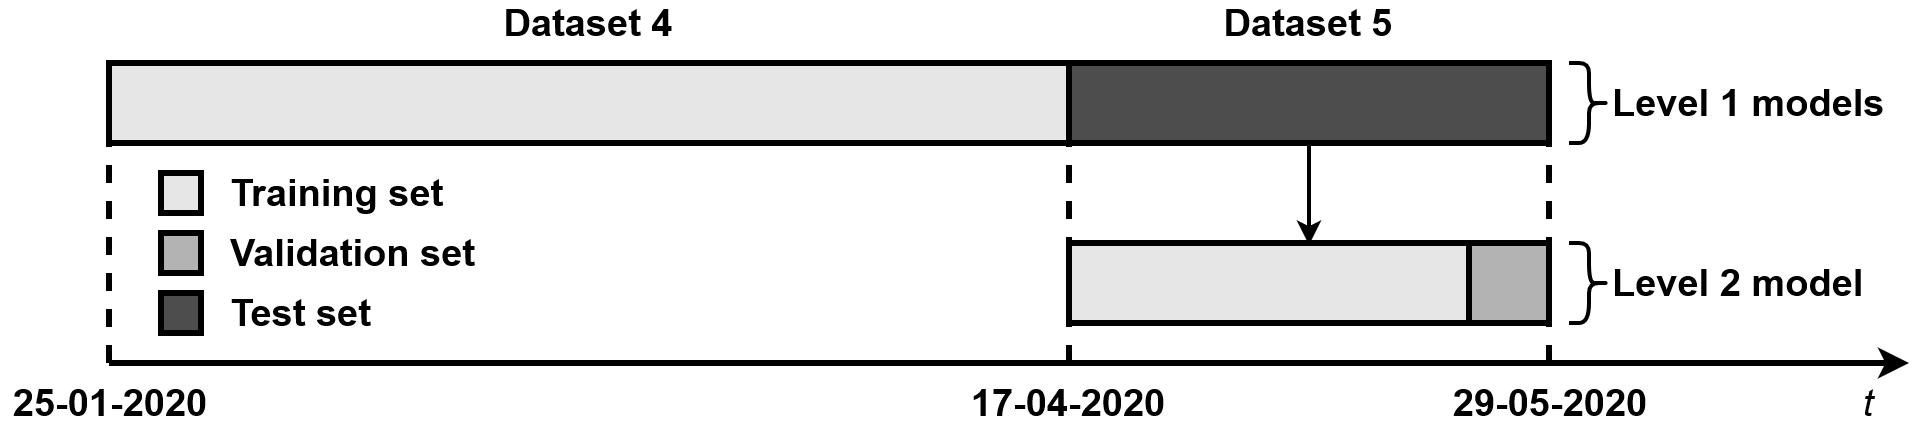
\includegraphics[width=1\textwidth]{Images/stage2.png}
    \caption{Dataset used for testing.}
    \label{level22}
    \end{center}
\end{figure}

The forecasts of (t+5), (t+10) and (t+15) of models 1, 2 and 3 of level 1, are used as input for the 
level 2 model and as targets, this model uses the measured values for the same instant to which the forecasts refer to ((t+5), (t+10) and (t+15)). Table \ref{table:Enseble} details the features used in this process.

\begin{table}[htbp]
  \centering
  \caption{Level 2 model features.}
    \begin{tabular}{rlcl}
    \toprule
          & \multicolumn{1}{c}{\textbf{Feature}} & \textbf{Unit} & \multicolumn{1}{c}{\textbf{Description}} \\
    \midrule
    Input & Model1\_(t+ 5) & W     & Available power prediction of Model 1 for 5 minutes ahead \\
          & Model1\_(t+ 10) & W     & Available power prediction of Model 1 for 10 minutes ahead \\
          & Model1\_(t+ 15) & W     & Available power prediction of Model 1 for 15 minutes ahead \\
          & Model2\_(t+ 5) & W     & Available power prediction of Model 2 for 5 minutes ahead \\
          & Model2\_(t+ 10) & W     & Available power prediction of Model 2 for 10 minutes ahead \\
          & Model2\_(t+ 15) & W     & Available power prediction of Model 2 for 15 minutes ahead \\
          & Model3\_(t+ 5) & W     & Available power prediction of Model 3 for 5 minutes ahead \\
          & Model3\_(t+ 10) & W     & Available power prediction of Model 3 for 10 minutes ahead \\
          & Model3\_(t+ 15) & W     & Available power prediction of Model 3 for 15 minutes ahead \\
    \midrule
    Output & Real (t+5) & W     & Real available power for 5 minutes ahead \\
          & Real (t+10) & W     & Real available power for 10 minutes ahead \\
          & Real (t+15) & W     & Real available power for 15 minutes ahead \\
    \end{tabular}%
  \label{table:Enseble}%
\end{table}%

As input variables, forecasts of each of the selected models of level 1 were chosen. As output variables, the same variables as those present in level 1, the available power in 5, 10 and 15 minutes, is used. Thus, it is necessary to create a model that can, based on the forecasts obtained for the instants (t+5), (t+10) and (t+15), generate new forecasting results for the same instants, using information mutually generated by the three models. By using more useful information, it is expected that a model that considers the results of three models simultaneously will perform better than a single model, and it is based on this premise that a hybrid system is then developed, which uses the outputs from one set of models as input from another.

\subsubsection{Model specifications}


In this second step, it is expected to create a model that, based on the data obtained for the instant (t+5), can obtain new data for (t+5), from the data obtained for the instant (t+10), can obtain new data for (t+10), and based on the data obtained for the instant (t+15), can obtain new data for (t+15). This means that it is no longer necessary to use a \ac{ANN} that can identify temporal patterns, but one that can simply establish a relationship between the input and output data, i.e. it is necessary to apply a simple \ac{FFNN}. 

As explained in section \ref{chap4:anns}, the best way to do this is to create a \ac{ANN} composed only by layers of the Dense type. In Table \ref{tab:level2arch}, a summary of the specifications of the four evaluated layouts for the level 2 model can be found.

\begin{table}[htbp]
  \centering
  \caption{Level 2 model specifications.}
    \begin{tabular}{c|cccc}
    \toprule
    \textbf{Model} & \multicolumn{4}{c}{Level 2 Model} \\
    \midrule
    Layout & 0     & 1      & 2     & 3 \\
    \midrule
          & Input (12) & Input (12) & Input (12) & Input (12) \\
          & Dense (8) & Dense (16) & Dense (32) & Dense (64) \\
          & Dense (8) & Dense (16) & Dense (32) & Dense (64) \\
          & Dense (3) & Dense (3) & Dense (3) & Dense (3) \\
    \midrule
    \# inputs & 12    & 12    & 12    & 12 \\
    \# hidden layers & 2     & 2     & 2     & 2 \\
    \# hidden nodes & 16    & 32    & 64    & 128 \\
    \# outputs & 3     & 3     & 3     & 3 \\
    \end{tabular}%
  \label{tab:level2arch}%
\end{table}%



For all four layouts studied, two hidden layers were used. The only hyperparameter that changed from layout to layout was the number of neurons (the size of the output space) in each of the layers. Combinations of two layers of 8 neurons each, two layers of 16 neurons each, two layers of 32 neurons each, and two layers of 64 neurons each were tested. After defining the structural details of the level 2 model layouts to be evaluated, a standard validation process was carried out in which data from the predictions computed by the three level 1 models (which correspond to the time interval of dataset 5), were divided into training and validation with a distribution of 75\% - 25\%, respectively, which represents approximately five weeks of data for testing and one week for validation. Table XXX shows the test and validation results for dataset 5, where the four layouts were trained and validated.









\subsection{Stage 3 - Results}

So far, both level 1 and level 2 models have been trained. In this third and final phase, the objective is to test the models created and compare their performance. Figure \ref{test} shows a distribution of the data used in this phase. The level 1 models were trained with the data collected between January 25, 2020 and April 17, 2020, and the level 2 model was trained with the forecasts made by these same level 1 models for the period between April 17, 2020 and May 29, 2020. It should be noted that the training periods have quite different dimensions,

\begin{figure}[h!]
    \centering
    \begin{center}
    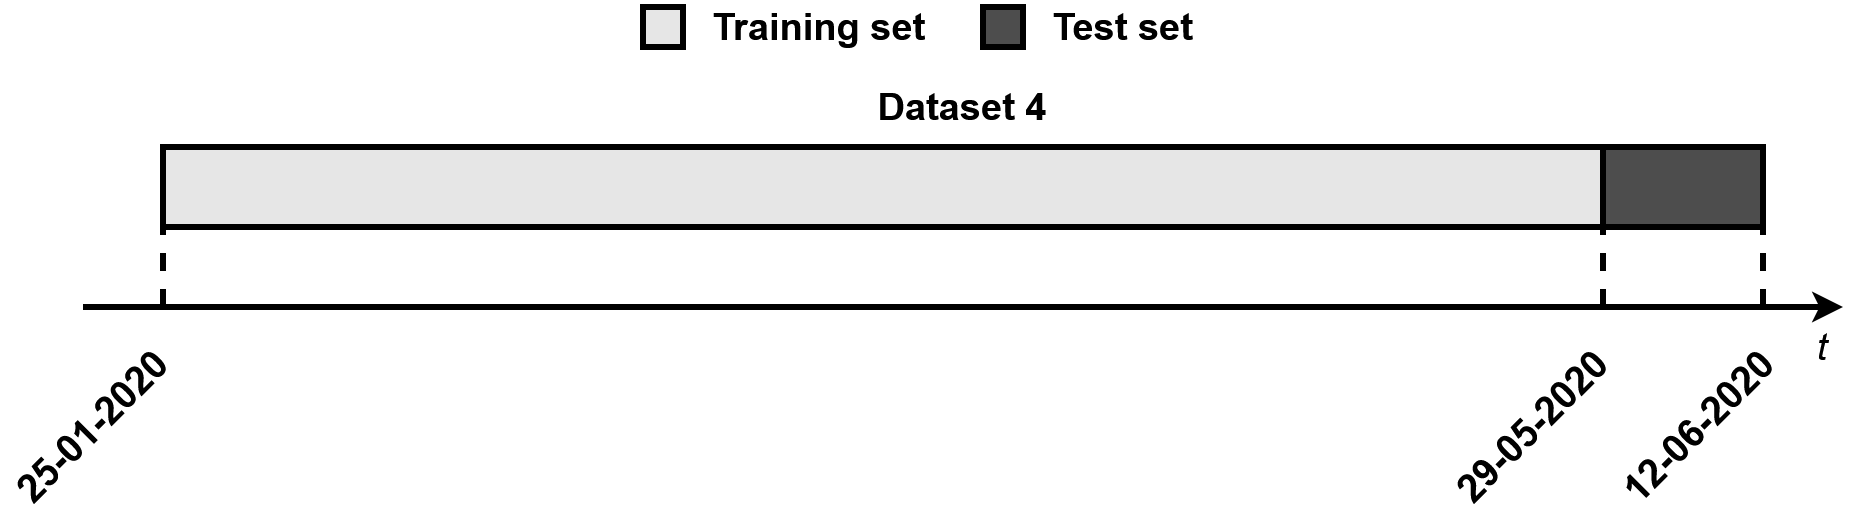
\includegraphics[width=1\textwidth]{Images/Test.png}
    \caption{Dataset used for testing.}
    \label{test}
    \end{center}
\end{figure}

\section{Discussion}



% If Printing on DOUBLE SIDED pages, the second page should be white.
% Otherwise, comment the following command:
%\cleardoublepage
%%Chapter 7
%% #############################################################################
% This is Chapter 7
% !TEX root = ../main.tex
% #############################################################################
% Change the Name of the Chapter i the following line
\fancychapter{Conclusions and Future Work}
\cleardoublepage
% The following line allows to ref this chapter
\label{chap:conclusion}

\section{Conclusions}
\section{Future Work}
% If Printing on DOUBLE SIDED pages, the second page should be white.
% Otherwise, comment the following command:
%\cleardoublepage
% -----------------------------------------------------------------------------
% BIBLIOGRAPHY
% Add the Bibliography to the PDF table of contents (not the document table of contents)
\pdfbookmark[0]{Bibliography}{bib}
% The bibliography style sheet
% Chose your preferences on the format of the entries and the Labels:
% IEEEtran: Used in general (recommended for IST Thesis)
%           Entries are labelled and sorted by appearance in the document
%           Labels are Numeric inside square brackets
\bibliographystyle{IEEEtran}
%
% Apalike:  Entries formatted alphabetically, last name first, with identation
%           Labels with Autor's Name and Year inside square brackets
%\bibliographystyle{apalike}
%
% Alpha:    Entries formatted with Autor's Name and Year, hanging identation
%           Labels with Autor's abbr. Names and Year inside square brackets
%\bibliographystyle{alpha}
%
% Acm:Entries formatted with Autor's Name (small Caps), hanging identation
%          Labels are Numeric inside square brackets
%\bibliographystyle{acm}
% The following command resets the 'emphasis' style for bibliography entries
\normalem
% Name of your BiBTeX file
\bibliography{./Thesis-MSc-Bibliography} % Put here your own filename
%
% The following command modifies the 'emphasis' style for bibliography entries
\ULforem
% If Printing on DOUBLE SIDED pages, the second page should be white.
% Otherwise, comment the following command:
\cleardoublepage
%
% -----------------------------------------------------------------------------
% HERE GO THE APPENDIXES IF REQUIRED
% If not required just comment the blocks
\appendix
%% First Appendix
\pdfbookmark[1]{Appendix A}{appendix}
% #############################################################################
% This is Appendix A
% !TEX root = ../main.tex
% #############################################################################
\chapter{Code of Project}
\label{chapter:appendixA}

Nulla dui purus, eleifend vel, consequat non, dictum porta, nulla. Duis ante mi, laoreet ut, commodo eleifend, cursus nec, lorem. Aenean eu est. Etiam imperdiet turpis. Praesent nec augue. Curabitur ligula quam, rutrum id, tempor sed, consequat ac, dui. Vestibulum accumsan eros nec magna. Vestibulum vitae dui. Vestibulum nec ligula et lorem consequat ullamcorper. 



\begin{lstlisting} [style=py,caption={PYTHON Code}]
class TelgramRequestHandler(object):
    def handle(self):
        addr = self.client_address[0]         # Client IP-adress
        telgram = self.request.recv(1024)     # Recieve telgram
        print "From: %s, Received: %s" % (addr, telgram)
        return
\end{lstlisting}
%% If Printing on DOUBLE SIDED pages, the second page should be white.
%% Otherwise, comment the following command:
\cleardoublepage

%% Second Appendix
\pdfbookmark[1]{Appendix B}{appendix}
% #############################################################################
% This is Appendix B
% !TEX root = ../main.tex
% #############################################################################
\chapter{Literature revision tables}


\label{chapter:appendixB}

This appendix includes a table with some details of scientific articles that study issues similar to the theme of this thesis.

\begin{landscape}

    \begin{longtable}{llllllll}
    \caption {Summary of ANNs in predicting building energy consumption.}
    \label{table1}\\
    \hline \\[-1.0ex]
    \textbf{Year} & \textbf{Reference} & \textbf{Type of building}  & \textbf{Inputs} & \textbf{Output} & \textbf{Dataset length} & \textbf{Model} \\[+1.0ex] \hline \\[-1.0ex]
    \endhead

     2000   &
     \cite{annr1}  &
     Supermarket & 
     \makecell*[{{p{5cm}}}]{~\textbullet~Day, Time, External Humidity and Temperature and Internal humidity and temperature for short term i.e. a month}   & 
     \makecell*[{{p{5cm}}}]{~\textbullet~Energy consumption}   & 
     Not specified  & 
     \makecell*[{{p{3cm}}}]{BPNN}  \\
     
     
     2000   &
     \cite{annr2}  &
     Holiday passive house  & 
     \makecell*[{{p{5cm}}}]{~\textbullet~Season, insulation function, wall thickness, heat transfer coefficient, time of day}   & 
     \makecell*[{{p{5cm}}}]{~\textbullet~Energy consumption}   & 
     Two seasons & 
     \makecell*[{{p{3cm}}}]{RNN combined with BPNN}  \\
         
     2005   &
     \cite{annr3}  &
     Office   & 
     \makecell*[{{p{5cm}}}]{~\textbullet~Outdoor dry-bulb temperature, outdoor humility, water temperature of chiller, compressor status etc.}   & 
     \makecell*[{{p{5cm}}}]{~\textbullet~Dynamic chiller electric demand}   & 
     1 year & 
     \makecell*[{{p{3cm}}}]{Sliding window ANN and accumulative ANN}  \\


     2005   &
     \cite{svm2}  &
     Commercial   & 
     \makecell*[{{p{5cm}}}]{~\textbullet~Outdoor temperature, relative humility, global solar
     radiation, previous electricity consumption}   & 
     \makecell*[{{p{5cm}}}]{~\textbullet~Building energy consumption per month} & 
     3 years & 
     \makecell*[{{p{3cm}}}]{SVM}   \\

         
     2007   &
     \cite{annr4}  &
     Multiple  & 
     \makecell*[{{p{5cm}}}]{~\textbullet~Economic indicators (GNP and GDP), population}   & 
     \makecell*[{{p{5cm}}}]{~\textbullet~Energy consumption}   & 
     37 years (1968–2005) & 
     \makecell*[{{p{3cm}}}]{BPNN}  \\    
     
     2008   &
     \cite{annr5}  &
     Solar house  & 
     \makecell*[{{p{5cm}}}]{~\textbullet~Outdoor temperature, relative humility, set point temperature, occupancy schedule}   & 
     \makecell*[{{p{5cm}}}]{~\textbullet~Heating/cooling consumption}   & 
     2 days & 
     \makecell*[{{p{3cm}}}]{BPNN}  \\
         
     2009   &
     \cite{annr6}  &
     Multiple & 
     \makecell*[{{p{5cm}}}]{~\textbullet~Transparency ratios, insulation thickness, building form factors and heating energy demands}   & 
     \makecell*[{{p{5cm}}}]{~\textbullet~Building heating energy requirements}   & 
     5 years  & 
     \makecell*[{{p{3cm}}}]{BPNN}  \\
     
     2009   &
     \cite{annr7}  &
     Commercial & 
     \makecell*[{{p{5cm}}}]{~\textbullet~Previous cooling demand, air temperature and relative humidity}   & 
     \makecell*[{{p{5cm}}}]{~\textbullet~Cooling demand}   & 
     45 weekdays & 
     \makecell*[{{p{3cm}}}]{BPNN}  \\   
     
     2009   &
     \cite{svm5}  &
     Office  & 
     \makecell*[{{p{5cm}}}]{~\textbullet~Outdoor weather parameters, the outdoor temperature, humidity and solar radiation}   & 
     \makecell*[{{p{5cm}}}]{~\textbullet~Building cooling load}   & 
     6 months & 
     \makecell*[{{p{3cm}}}]{BPNN, RBFNN, RNN and SVM} \\
     
     2009   &
     \cite{svmr0}  &
     Multiple   & 
     \makecell*[{{p{5cm}}}]{~\textbullet~Historical electricity consumption data}   & 
     \makecell*[{{p{5cm}}}]{~\textbullet~5-min ahead electricity load} & 
     3 years & 
     \makecell*[{{p{3cm}}}]{SVM, statistical regression, and BPNN}  \\
     
     2009   &
     \cite{svmr1}  &
     Not specified   & 
     \makecell*[{{p{5cm}}}]{~\textbullet~Past energy consumption, past climatic data}   & 
     \makecell*[{{p{5cm}}}]{~\textbullet~Energy load}   & 
     Not specified & 
     \makecell*[{{p{3cm}}}]{SVM}  \\
     
     2010   &
     \cite{annr8}  &
     Residential & 
     \makecell*[{{p{5cm}}}]{~\textbullet~18 building envelope parameters, heating degree day, cooling degree day}   & 
     \makecell*[{{p{5cm}}}]{~\textbullet~Heating and cooling energy consumption}   & 
     1 year & 
     \makecell*[{{p{3cm}}}]{BPNN}  \\   
     
     2010   &
     \cite{svm3}  &
     Office buildings   & 
     \makecell*[{{p{5cm}}}]{~\textbullet~Heating consumption, electrical consumption}   & 
     \makecell*[{{p{5cm}}}]{~\textbullet~Heating demand and electrical load} & 
     5 months & 
     \makecell*[{{p{3cm}}}]{Parallel SVM}   \\
     
     2010   &
     \cite{svmr2}  &
     Office buildings   & 
     \makecell*[{{p{5cm}}}]{~\textbullet~Past building cooling load}   & 
     \makecell*[{{p{5cm}}}]{~\textbullet~Building cooling load}   & 
     6 months & 
     \makecell*[{{p{3cm}}}]{FSVM} \\ 
     
     2011   &
     \cite{annr9}  &
     Multiple & 
     \makecell*[{{p{5cm}}}]{~\textbullet~Weather conditions, calendar, type of day and other factors}&
     \makecell*[{{p{5cm}}}]{~\textbullet~Energy consumption}   & 
     1 year & 
     \makecell*[{{p{3cm}}}]{BPNN}  \\
     
     2012  &
     \cite{svmr3}  &
     Residential & 
     \makecell*[{{p{5cm}}}]{~\textbullet~Past energy consumption, past climatic data}   & 
     \makecell*[{{p{5cm}}}]{~\textbullet~Energy consumption}   & 
     2 years & 
     \makecell*[{{p{3cm}}}]{SVM and SVR} \\     
     
     2013   &
     \cite{annr10}  &
     Multiple & 
     \makecell*[{{p{5cm}}}]{~\textbullet~Previous electricity consumption}   & 
     \makecell*[{{p{5cm}}}]{~\textbullet~Half-hour ahead electricity demand}   & 
     9 weeks & 
     \makecell*[{{p{3cm}}}]{Multi-output BPNN}  \\
     
     2015   &
     \cite{annr12}  &
     Multiple & 
     \makecell*[{{p{5cm}}}]{~\textbullet~Outdoor and indoor temperature, solar radiation, humidity ratio, wind speed, occupancy}   & 
     \makecell*[{{p{5cm}}}]{~\textbullet~Building electricity power consumption}   & 
     6 months & 
     \makecell*[{{p{3cm}}}]{Hybrid iPSO-ANN and GA-ANN}  \\
     
     2015   &
     \cite{regression0}  &
     Residential & 
     \makecell*[{{p{5cm}}}]{~\textbullet~Energy consumption, time, outdoor temperature and global horizon radiation}   & 
     \makecell*[{{p{5cm}}}]{~\textbullet~Energy consumption}   & 
     1 month & 
     \makecell*[{{p{3cm}}}]{Simple and multiple regression analysis}  \\
     
      2016   &
     \cite{annr13}  &
     Commercial & 
     \makecell*[{{p{5cm}}}]{~\textbullet~Meteorological data and HVAC operation schedule}   & 
     \makecell*[{{p{5cm}}}]{~\textbullet~Energy consumption}   & 
     1 year & 
     \makecell*[{{p{3cm}}}]{BPNN}  \\    
     
      2016   &
     \cite{annr14}  &
     Office & 
     \makecell*[{{p{5cm}}}]{~\textbullet~Previous load, temperatures of previous day, occupancy condition, sin and cosine of the hour}   & 
     \makecell*[{{p{5cm}}}]{~\textbullet~One day ahead electric power consumption}   & 
     1 year and a half & 
     \makecell*[{{p{3cm}}}]{BPNN}  \\
      
     2016   &
     \cite{svmr4}  &
     Institutional  & 
     \makecell*[{{p{5cm}}}]{~\textbullet~Daily and half-hourly energy consumption}   & 
     \makecell*[{{p{5cm}}}]{~\textbullet~Daily and half-hourly energy consumption} & 
     1 year & 
     \makecell*[{{p{3cm}}}]{GA combined with SVM}   \\
     
     2016   &
     \cite{annr15}  &
     Institutional & 
     \makecell*[{{p{5cm}}}]{~\textbullet~Indoor conditions and occupancy}   & 
     \makecell*[{{p{5cm}}}]{~\textbullet~Energy consumption}   & 
     1 to 2 years & 
     \makecell*[{{p{3cm}}}]{RNN}  \\
     
     2016   &
     \cite{annr22}  &
     University & 
     \makecell*[{{p{5cm}}}]{~\textbullet~Energy consumption and temperature}   & 
     \makecell*[{{p{5cm}}}]{~\textbullet~Energy consumption}   & 
     1 year & 
     \makecell*[{{p{3cm}}}]{Non-linear auto regressive model}  \\

      2017   &
     \cite{annr16}  &
     Residential & 
     \makecell*[{{p{5cm}}}]{~\textbullet~Past energy consumption}   & 
     \makecell*[{{p{5cm}}}]{~\textbullet~Energy consumption}   & 
     1 year and a half & 
     \makecell*[{{p{3cm}}}]{PDRNN}  \\ 
     
      2017   &
     \cite{annr17}  &
     Office & 
     \makecell*[{{p{5cm}}}]{~\textbullet~Past energy consumption, past climatic data}   & 
     \makecell*[{{p{5cm}}}]{~\textbullet~Energy consumption}   & 
     1 year  & 
     \makecell*[{{p{3cm}}}]{BPNN}  \\
     
     2017   &
     \cite{annr18}  &
     Not specified & 
     \makecell*[{{p{5cm}}}]{~\textbullet~Past energy load, past climatic data}   & 
     \makecell*[{{p{5cm}}}]{~\textbullet~Load forecast}   & 
     Not specified & 
     \makecell*[{{p{3cm}}}]{DNN}  \\    
     
     2017   &
     \cite{svmr7}  &
     Residential & 
     \makecell*[{{p{5cm}}}]{~\textbullet~Climatic data}   & 
     \makecell*[{{p{5cm}}}]{~\textbullet~Energy consumption}   & 
     Not specified & 
     \makecell*[{{p{3cm}}}]{SVM}  \\    
     
     2018   &
     \cite{annr19}  &
     Residential & 
     \makecell*[{{p{5cm}}}]{~\textbullet~Socio-demographic data, building characteristics, occupancy and appliance characteristics}   & 
     \makecell*[{{p{5cm}}}]{~\textbullet~Energy consumption}   & 
     Not specified & 
     \makecell*[{{p{3cm}}}]{BPNN}  \\
     
     2018   &
     \cite{annr20}  &
     Office & 
     \makecell*[{{p{5cm}}}]{~\textbullet~Past energy consumption, air-conditioning data, operating hours, other consumption sources}   & 
     \makecell*[{{p{5cm}}}]{~\textbullet~HVAC related energy saving}   & 
     15 years & 
     \makecell*[{{p{3cm}}}]{BPNN}  \\ 
     
     
     2018   &
     \cite{annr24}  &
     Multiple & 
     \makecell*[{{p{5cm}}}]{~\textbullet~Climatic data, calendar, occupation}   & 
     \makecell*[{{p{5cm}}}]{~\textbullet~Energy  consumption}   & 
     6 months & 
     \makecell*[{{p{3cm}}}]{Improved teaching learning based optimization algorithm based artificial neural network}  \\ 
     
     2018   &
     \cite{annr25}  &
     University & 
     \makecell*[{{p{5cm}}}]{~\textbullet~Past energy consumption and climatic data}   & 
     \makecell*[{{p{5cm}}}]{~\textbullet~Energy  consumption}   & 
     Not specified & 
     \makecell*[{{p{3cm}}}]{ANNs}  \\ 
     
     2018   &
     \cite{svmr5}  &
     Not specified & 
     \makecell*[{{p{5cm}}}]{~\textbullet~Climatic data, ratio  of  urbanization,  gross  domestic  product, household consumption level and total area of structure}   & 
     \makecell*[{{p{5cm}}}]{~\textbullet~Energy consumption} & 
     14 years & 
     \makecell*[{{p{3cm}}}]{SVM}   \\ 
     
     2018   &
     \cite{dt0}  &
     Multiple & 
     \makecell*[{{p{5cm}}}]{~\textbullet~Climatic data}   & 
     \makecell*[{{p{5cm}}}]{~\textbullet~Energy consumption} & 
     1 year & 
     \makecell*[{{p{3cm}}}]{DTs, Regressive models}   \\ 
     
     2018   &
     \cite{rf0}  &
     Multiple & 
     \makecell*[{{p{5cm}}}]{~\textbullet~Climatic data, occupancy, schedule}   & 
     \makecell*[{{p{5cm}}}]{~\textbullet~Energy consumption} & 
     1 year & 
     \makecell*[{{p{3cm}}}]{Random forest}   \\ 
          
     2019   &
     \cite{annr21}  &
     Multiple & 
     \makecell*[{{p{5cm}}}]{~\textbullet~Past energy consumption, past climatic data}   & 
     \makecell*[{{p{5cm}}}]{~\textbullet~Energy consumption}   & 
     4 years & 
     \makecell*[{{p{3cm}}}]{RNN, SSA and TCNN}  \\  
     
     2019   &
     \cite{annr26}  &
     Educational & 
     \makecell*[{{p{5cm}}}]{~\textbullet~Climatic data, occupancy, schedule, operating variables}   & 
     \makecell*[{{p{5cm}}}]{~\textbullet~Energy consumption}   & 
     1 year & 
     \makecell*[{{p{3cm}}}]{RNN, LSTM and GRU}  \\  
     
     2019   &
     \cite{annr27}  &
     Multiple & 
     \makecell*[{{p{5cm}}}]{~\textbullet~Hubei province, China (Energy consumption, temporal and climatic data)}   & 
     \makecell*[{{p{5cm}}}]{~\textbullet~Power load forecasting}   & 
     11 months & 
     \makecell*[{{p{3cm}}}]{Variational mode decomposition, LSTMs and Bayesian optimization algorithm}  \\  
     
     2019   &
     \cite{annr28}  &
     Multiple& 
     \makecell*[{{p{5cm}}}]{~\textbullet~Energy consumption data from five states of Australia}   & 
     \makecell*[{{p{5cm}}}]{~\textbullet~Power load forecasting}   & 
     Not specified & 
     \makecell*[{{p{3cm}}}]{ANNs, BPNN, GABPNN, ELM and GRNN}  \\  
     
     2019   &
     \cite{annr29}  &
     Residential & 
     \makecell*[{{p{5cm}}}]{~\textbullet~Schedule, Global active power, average voltage}   & 
     \makecell*[{{p{5cm}}}]{~\textbullet~Energy consumption}   & 
     4 years & 
     \makecell*[{{p{3cm}}}]{CNNs and LSTMs}  \\  
     
     2019   &
     \cite{svmr6}  &
      Office  & 
     \makecell*[{{p{5cm}}}]{~\textbullet~Not specified}   & 
     \makecell*[{{p{5cm}}}]{~\textbullet~Energy consumption} & 
     2 months & 
     \makecell*[{{p{3cm}}}]{SVR}   \\ 
     
     2019   &
     \cite{other1}  &
     Educational  & 
     \makecell*[{{p{5cm}}}]{~\textbullet~Schedule, climatic data and other operating parameters}   & 
     \makecell*[{{p{5cm}}}]{~\textbullet~Energy consumption} & 
     1 year & 
     \makecell*[{{p{3cm}}}]{Deep learning techniques for feature engineering}  \\  
     
     2019   &
     \cite{other2}  &
     Multiple  & 
     \makecell*[{{p{5cm}}}]{~\textbullet~physical characteristics of the building and independent of the climate}   & 
     \makecell*[{{p{5cm}}}]{~\textbullet~Energy consumption} & 
     Not specified & 
     \makecell*[{{p{3cm}}}]{ANNs, SVMs, Gaussian Process, RF and DTs}   \\             


    \end{longtable}

\end{landscape}
%% If Printing on DOUBLE SIDED pages, the second page should be white.
%% Otherwise, comment the following command:
\cleardoublepage

\pdfbookmark[1]{Appendix E}{appendix}
% #############################################################################
% This is Appendix E
% !TEX root = ../main.tex
% #############################################################################
\chapter{Data}
\label{chapter:appendixE}


This appendix contains the tables concerning the features computed and the features made available for the development of this thesis. Table \ref{tab:available_variables} contains the four datasets provided by \ac{FCUL} and by \ac{EDP}, where the name of each feature, the unit in which it is found, and a brief description are discriminated. 

\newpage

\begin{table}[htbp]
  \centering
  \scriptsize
  \caption{Description of the provided and computed variables.}
    \begin{tabular}{lcl|rrr}
    \textbf{Meteo.} &   &   & \multicolumn{1}{l}{\textbf{Rad.}} &   &  \\
    \textbf{Feature} & \textbf{Unit} & \textbf{Description} & \multicolumn{1}{l}{\textbf{Feature}} & \multicolumn{1}{c}{\textbf{Unit}} & \multicolumn{1}{l}{\textbf{Description}} \\
    \midrule
    T\_amb\_min & degC & Minimum ambient temperature & \multicolumn{1}{l}{Avg\_GHI} & \multicolumn{1}{c}{W/m2} & \multicolumn{1}{l}{Average global horizontal irradiance} \\
    T\_amb\_max & degC & Maximum ambient temperature & \multicolumn{1}{l}{Avg\_DHI} & \multicolumn{1}{c}{W/m2} & \multicolumn{1}{l}{Average diffuse horizontal irradiance} \\
    T\_amb\_avg & degC & Average ambient temperature & \multicolumn{1}{l}{Avg\_POA} & \multicolumn{1}{c}{W/m2} & \multicolumn{1}{l}{Average plane of array} \\
    T\_dp\_avg & degC & Time-dependenta verage temperature & \multicolumn{1}{l}{Avg\_DNI} & \multicolumn{1}{c}{W/m2} & \multicolumn{1}{l}{Average direct normal irradiance} \\
    RH\_min & \% & Minimum relative humidity & \multicolumn{1}{l}{Avg\_cosDNI} & \multicolumn{1}{c}{W/m2} & \multicolumn{1}{l}{Cos theta correction} \\
    RH\_max & \% & Maximum relative humidity & \multicolumn{1}{l}{Avg\_closGHI} & \multicolumn{1}{c}{W/m2} & \multicolumn{1}{l}{Cos theta correction} \\
    RH\_avg & \% & Average relative humidity & \multicolumn{1}{l}{Std\_GHI} & \multicolumn{1}{c}{W/m2} & \multicolumn{1}{l}{Standard global horizontal irradiance} \\
    AH\_min & g/m3 & Minimum absolute humidity & \multicolumn{1}{l}{Std\_DHI} & \multicolumn{1}{c}{W/m2} & \multicolumn{1}{l}{Standard diffuse horizontal irradiance} \\
    AH\_max & g/m3 & Maximum absolute humidity & \multicolumn{1}{l}{Std\_POA} & \multicolumn{1}{c}{W/m2} & \multicolumn{1}{l}{Standard plane of array} \\
    AH\_avg & g/m3 & Average absolute humidity & \multicolumn{1}{l}{Std\_DNI} & \multicolumn{1}{c}{W/m2} & \multicolumn{1}{l}{Standard direct normal irradiance} \\
    p\_amb\_min & hPa & Minimum atmospheric pressure & \multicolumn{1}{l}{Std\_cosDNI} & \multicolumn{1}{c}{W/m2} & \multicolumn{1}{l}{Cos theta correction} \\
    p\_amb\_max & hPa & Maximum atmospheric pressure & \multicolumn{1}{l}{Std\_closGHI} & \multicolumn{1}{c}{W/m2} & \multicolumn{1}{l}{Cos theta correction} \\
    p\_amb\_avg & hPa & Average atmospheric pressure & \multicolumn{1}{l}{Min\_GHI} & \multicolumn{1}{c}{W/m2} & \multicolumn{1}{l}{Minimum global horizontal irradiance} \\
    rho\_act & kg/m3 & Air density & \multicolumn{1}{l}{Min\_DHI} & \multicolumn{1}{c}{W/m2} & \multicolumn{1}{l}{Minimum diffuse horizontal irradiance} \\
    v\_min & m/s & Minimum air speed & \multicolumn{1}{l}{Min\_POA} & \multicolumn{1}{c}{W/m2} & \multicolumn{1}{l}{Minimum plane of array} \\
    v\_max & m/s & Maximum air speed & \multicolumn{1}{l}{Min\_DNI} & \multicolumn{1}{c}{W/m2} & \multicolumn{1}{l}{Minimum direct normal irradiance} \\
    v\_avg & m/s & Average air speed & \multicolumn{1}{l}{Min\_cosDNI} & \multicolumn{1}{c}{W/m2} & \multicolumn{1}{l}{Cos theta correction} \\
    v\_vectavg & m/s & Average gust speed & \multicolumn{1}{l}{Min\_closGHI} & \multicolumn{1}{c}{W/m2} & \multicolumn{1}{l}{Cos theta correction} \\
    v\_dir\_min & degrees & Minimum wind direction & \multicolumn{1}{l}{Max\_GHI} & \multicolumn{1}{c}{W/m2} & \multicolumn{1}{l}{Maximum global horizontal irradiance} \\
    v\_dir\_max & degrees & Maximum wind direction & \multicolumn{1}{l}{Max\_DHI} & \multicolumn{1}{c}{W/m2} & \multicolumn{1}{l}{Maximum diffuse horizontal irradiance} \\
    v\_dir\_vectavg & degrees & Average wind direction & \multicolumn{1}{l}{Max\_POA} & \multicolumn{1}{c}{W/m2} & \multicolumn{1}{l}{Maximum plane of array} \\
\cmidrule{1-3}    \textbf{Prod.} &   &   & \multicolumn{1}{l}{Max\_DNI} & \multicolumn{1}{c}{W/m2} & \multicolumn{1}{l}{Maximum direct normal irradiance} \\
    \textbf{Feature} & \textbf{Unit} & \textbf{Description} & \multicolumn{1}{l}{Max\_cosDNI} & \multicolumn{1}{c}{W/m2} & \multicolumn{1}{l}{Cos theta correction} \\
\cmidrule{1-3}    I1 & A & Production three-phase current & \multicolumn{1}{l}{Max\_closGHI} & \multicolumn{1}{c}{W/m2} & \multicolumn{1}{l}{Cos theta correction} \\
    I2 & A & Production three-phase current & \multicolumn{1}{l}{phi} & \multicolumn{1}{c}{degree} & \multicolumn{1}{l}{azimuth angle} \\
    I3 & A & Production three-phase current & \multicolumn{1}{l}{theta} & \multicolumn{1}{c}{degree} & \multicolumn{1}{l}{zenit angle} \\
    V1 & V & Production three-phase voltage & \multicolumn{1}{l}{SensorT} & \multicolumn{1}{c}{degC} & \multicolumn{1}{l}{Sensor temperature} \\
    V2 & V & Production three-phase voltage &   &   &  \\
    V3 & V & Production three-phase voltage &   &   &  \\
    ActPwr & W & Production active power &   &   &  \\
    \midrule
    \textbf{Cons.} &   &   & \multicolumn{1}{l}{\textbf{Computed}} &   &  \\
    \textbf{Feature} & \textbf{Unit} & \textbf{Description} & \multicolumn{1}{l}{\textbf{Feature}} & \multicolumn{1}{c}{\textbf{Unit}} & \multicolumn{1}{l}{\textbf{Description}} \\
    \midrule
    Ir & A & Consumption three-phase current & \multicolumn{1}{l}{hour} & \multicolumn{1}{c}{hours} & \multicolumn{1}{l}{Hour of the day} \\
    Is & A & Consumption three-phase current & \multicolumn{1}{l}{day\_of\_moth} & \multicolumn{1}{c}{days} & \multicolumn{1}{l}{Day of the month} \\
    It & A & Consumption three-phase current & \multicolumn{1}{l}{day\_of\_week} & \multicolumn{1}{c}{days} & \multicolumn{1}{l}{Day of the week} \\
    Vrs & V & Consumption three-phase voltage & \multicolumn{1}{l}{month} & \multicolumn{1}{c}{months} & \multicolumn{1}{l}{Month of the year} \\
    Vst & V & Consumption three-phase voltage & \multicolumn{1}{l}{holiday} & \multicolumn{1}{c}{binary} & \multicolumn{1}{l}{National holiday identifier} \\
    Vtr & V & Consumption three-phase voltage & \multicolumn{1}{l}{AvailablePower} & \multicolumn{1}{c}{W} & \multicolumn{1}{l}{Current available power} \\
    P & W & Consumption real power & \multicolumn{1}{l}{TheoreticalValue} & \multicolumn{1}{c}{W} & \multicolumn{1}{l}{Theoretical production active power} \\
    S & VA & Consumption complex power &   &   &  \\
    \end{tabular}%
  \label{tab:available_variables}%
\end{table}%


%% If Printing on DOUBLE SIDED pages, the second page should be white.
%% Otherwise, comment the following command:
\cleardoublepage

%% Second Appendix
%\pdfbookmark[1]{Appendix C}{appendix}
%% #############################################################################
% This is Appendix C
% !TEX root = ../main.tex
% #############################################################################
\chapter{Forecasting Results}


\label{chapter:appendixC}

This appendix includes a table with some details of scientific articles that study issues similar to the theme of this thesis.



\begin{landscape}
\begin{longtable}{|l|c|c|c|c|c|c|c|c|c|c|c|c|c|c|c|}
     \caption{Part 1 testing results}
     \label{table7}\\
    \toprule
    \multicolumn{1}{|c|}{\multirow{3}[2]{*}{\textbf{Model}}} & \multicolumn{3}{c|}{\textbf{Dataset 1 validation}} & \multicolumn{3}{c|}{\textbf{Dataset 2 validation}} & \multicolumn{3}{c|}{\textbf{Dataset 3 validation}} & \multicolumn{3}{c|}{\textbf{Total}} \\
          & \multirow{2}[1]{*}{\textbf{MSE}} & \multirow{2}[1]{*}{\textbf{RMSE}} & \multirow{2}[1]{*}{\textbf{MAE}} & \multirow{2}[1]{*}{\textbf{MSE}} & \multirow{2}[1]{*}{\textbf{RMSE}} & \multirow{2}[1]{*}{\textbf{MAE}} & \multirow{2}[1]{*}{\textbf{MSE}} & \multirow{2}[1]{*}{\textbf{RMSE}} & \multirow{2}[1]{*}{\textbf{MAE}} & \multirow{2}[1]{*}{\textbf{MSE}} & \multirow{2}[1]{*}{\textbf{RMSE}} & \multirow{2}[1]{*}{\textbf{MAE}} \\
          &       &       &       &       &       &       &       &       &       &       &       &  \\
    \midrule
    \endhead
    GRU-8 & 6.052E+04 & 3.663E+09 & 0.0740 & 2.053E+05 & 4.216E+10 & 0.4240 & 5.512E+04 & 3.038E+09 & 0.0938 & 1.070E+05 & 1.629E+10 & 0.1973 \\
    GRU-16 & \cellcolor[rgb]{ .573,  .816,  .314}\textbf{5.123E+04} & \cellcolor[rgb]{ .573,  .816,  .314}\textbf{2.625E+09} & 0.0687 & 1.772E+05 & 3.141E+10 & 0.3423 & 7.163E+04 & 5.131E+09 & 0.1323 & 1.000E+05 & 1.306E+10 & 0.1811 \\
    GRU-32 & 5.416E+04 & 2.933E+09 & 0.0702 & 1.769E+05 & 3.129E+10 & 0.3345 & 2.066E+05 & 4.267E+10 & 0.4240 & 1.459E+05 & 2.563E+10 & 0.2762 \\
    GRU-64 & 5.694E+04 & 3.242E+09 & 0.0704 & \cellcolor[rgb]{ .573,  .816,  .314}\textbf{8.088E+04} & \cellcolor[rgb]{ .573,  .816,  .314}\textbf{6.541E+09} & 0.1284 & \cellcolor[rgb]{ .573,  .816,  .314}\textbf{4.984E+04} & \cellcolor[rgb]{ .573,  .816,  .314}\textbf{2.484E+09} & \cellcolor[rgb]{ .573,  .816,  .314}\textbf{0.0826} & \cellcolor[rgb]{ .573,  .816,  .314}\textbf{6.255E+04} & \cellcolor[rgb]{ .573,  .816,  .314}\textbf{4.089E+09} & \cellcolor[rgb]{ .573,  .816,  .314}\textbf{0.0938} \\
    GRU-128 & 5.135E+04 & 2.637E+09 & \cellcolor[rgb]{ .573,  .816,  .314}\textbf{0.0677} & 8.703E+04 & 7.575E+09 & \cellcolor[rgb]{ .573,  .816,  .314}\textbf{0.1282} & 1.514E+05 & 2.291E+10 & 0.2817 & 9.658E+04 & 1.104E+10 & 0.1592 \\
    GRU-256 & 5.714E+04 & 3.265E+09 & 0.0727 & 1.894E+05 & 3.588E+10 & 0.3661 & 6.074E+04 & 3.689E+09 & 0.0933 & 1.024E+05 & 1.428E+10 & 0.1774 \\
    GRU-512 & 6.356E+04 & 4.039E+09 & 0.0791 & 1.620E+05 & 2.625E+10 & 0.2898 & 1.254E+05 & 1.571E+10 & 0.1897 & 1.170E+05 & 1.533E+10 & 0.1862 \\
    \midrule
    LSTM-8 & 8.918E+04 & 7.953E+09 & 0.1061 & 9.462E+04 & 8.953E+09 & 0.1912 & 1.317E+05 & 1.735E+10 & 0.2335 & \cellcolor[rgb]{ .573,  .816,  .314}\textbf{1.052E+05} & \cellcolor[rgb]{ .573,  .816,  .314}\textbf{1.142E+10} & 0.1769 \\
    LSTM-16 & 8.250E+04 & 6.807E+09 & 0.0974 & 1.346E+05 & 1.812E+10 & 0.2443 & 1.532E+05 & 2.346E+10 & 0.3076 & 1.234E+05 & 1.613E+10 & 0.2164 \\
    LSTM-32 & 1.178E+05 & 1.388E+10 & 0.1405 & \cellcolor[rgb]{ .573,  .816,  .314}\textbf{6.151E+04} & \cellcolor[rgb]{ .573,  .816,  .314}\textbf{3.783E+09} & \cellcolor[rgb]{ .573,  .816,  .314}\textbf{0.1149} & 2.755E+05 & 7.592E+10 & 0.5672 & 1.516E+05 & 3.119E+10 & 0.2742 \\
    LSTM-64 & 1.071E+05 & 1.147E+10 & 0.1296 & 1.932E+05 & 3.733E+10 & 0.3728 & \cellcolor[rgb]{ .573,  .816,  .314}\textbf{1.073E+05} & \cellcolor[rgb]{ .573,  .816,  .314}\textbf{1.151E+10} & 0.2053 & 1.359E+05 & 2.010E+10 & 0.2359 \\
    LSTM-128 & 6.690E+04 & 4.475E+09 & 0.0805 & 1.784E+05 & 3.184E+10 & 0.3099 & 1.694E+05 & 2.870E+10 & 0.2795 & 1.383E+05 & 2.167E+10 & 0.2233 \\
    LSTM-256 & 6.085E+04 & 3.703E+09 & 0.0755 & 1.394E+05 & 1.943E+10 & 0.2238 & 1.721E+05 & 2.961E+10 & 0.2727 & 1.241E+05 & 1.758E+10 & 0.1907 \\
    LSTM-512 & \cellcolor[rgb]{ .573,  .816,  .314}\textbf{5.777E+04} & \cellcolor[rgb]{ .573,  .816,  .314}\textbf{3.338E+09} & \cellcolor[rgb]{ .573,  .816,  .314}\textbf{0.0731} & 1.491E+05 & 2.224E+10 & 0.2499 & 1.258E+05 & 1.583E+10 & \cellcolor[rgb]{ .573,  .816,  .314}\textbf{0.1963} & 1.109E+05 & 1.380E+10 & \cellcolor[rgb]{ .573,  .816,  .314}\textbf{0.1731} \\
    \midrule
    1D-8-10-GRU-8 & 6.410E+04 & 4.109E+09 & 0.0808 & 1.586E+05 & 2.516E+10 & 0.2985 & 1.111E+05 & 1.234E+10 & 0.2182 & 1.113E+05 & 1.387E+10 & 0.1992 \\
    1D-8-10-GRU-16 & 5.662E+04 & 3.206E+09 & 0.0683 & 1.408E+05 & 1.984E+10 & 0.2669 & 1.034E+05 & 1.069E+10 & 0.2012 & 1.003E+05 & 1.124E+10 & 0.1788 \\
    1D-8-10-GRU-32 & 5.482E+04 & 3.005E+09 & 0.0722 & 1.432E+05 & 2.051E+10 & 0.2749 & 1.154E+05 & 1.333E+10 & 0.2232 & 1.045E+05 & 1.228E+10 & 0.1901 \\
    1D-8-10-GRU-64 & 6.140E+04 & 3.770E+09 & 0.0797 & 1.522E+05 & 2.315E+10 & 0.2868 & 8.648E+04 & 7.479E+09 & 0.1543 & 1.000E+05 & 1.147E+10 & 0.1736 \\
    1D-8-10-GRU-128 & 5.785E+04 & 3.347E+09 & 0.0731 & 1.665E+05 & 2.772E+10 & 0.3216 & 6.614E+04 & 4.374E+09 & 0.1069 & 9.683E+04 & 1.182E+10 & 0.1672 \\
    1D-8-10-GRU-256 & 6.485E+04 & 4.205E+09 & 0.0824 & 1.975E+05 & 3.902E+10 & 0.3850 & 7.781E+04 & 6.054E+09 & 0.1226 & 1.134E+05 & 1.643E+10 & 0.1966 \\
    1D-16-10-GRU-8 & 7.282E+04 & 5.303E+09 & 0.0935 & 1.830E+05 & 3.348E+10 & 0.3508 & 8.193E+04 & 6.713E+09 & 0.1250 & 1.126E+05 & 1.516E+10 & 0.1898 \\
    1D-16-10-GRU-16 & 5.981E+04 & 3.578E+09 & 0.0719 & 1.717E+05 & 2.947E+10 & 0.3351 & 1.234E+05 & 1.524E+10 & 0.2432 & 1.183E+05 & 1.610E+10 & 0.2167 \\
    1D-16-10-GRU-32 & 5.998E+04 & 3.598E+09 & 0.0766 & 1.765E+05 & 3.115E+10 & 0.3413 & 8.494E+04 & 7.216E+09 & 0.1607 & 1.071E+05 & 1.399E+10 & 0.1929 \\
    1D-16-10-GRU-64 & 6.106E+04 & 3.728E+09 & 0.0723 & 1.689E+05 & 2.853E+10 & 0.3268 & 1.963E+05 & 3.852E+10 & 0.4012 & 1.421E+05 & 2.359E+10 & 0.2667 \\
    1D-16-10-GRU-128 & 6.027E+04 & 3.632E+09 & 0.0770 & 1.774E+05 & 3.146E+10 & 0.3425 & 7.726E+04 & 5.969E+09 & 0.1234 & 1.050E+05 & 1.369E+10 & 0.1810 \\
    1D-16-10-GRU-256 & 6.494E+04 & 4.217E+09 & 0.0817 & 1.773E+05 & 3.143E+10 & 0.3443 & 8.758E+04 & 7.670E+09 & 0.1317 & 1.099E+05 & 1.444E+10 & 0.1859 \\
    1D-32-10-GRU-8 & 5.831E+04 & 3.400E+09 & 0.0704 & 1.816E+05 & 3.297E+10 & 0.3525 & 1.523E+05 & 2.320E+10 & 0.3030 & 1.307E+05 & 1.986E+10 & 0.2420 \\
    1D-32-10-GRU-16 & 5.931E+04 & 3.517E+09 & 0.0740 & 1.831E+05 & 3.352E+10 & 0.3494 & 6.278E+04 & 3.942E+09 & 0.0995 & 1.017E+05 & 1.366E+10 & 0.1743 \\
    1D-32-10-GRU-32 & 5.903E+04 & 3.485E+09 & 0.0709 & 1.628E+05 & 2.650E+10 & 0.3078 & 1.440E+05 & 2.074E+10 & 0.2863 & 1.219E+05 & 1.691E+10 & 0.2217 \\
    1D-32-10-GRU-64 & 6.448E+04 & 4.157E+09 & 0.0821 & 1.688E+05 & 2.848E+10 & 0.3272 & 1.206E+05 & 1.455E+10 & 0.1856 & 1.180E+05 & 1.573E+10 & 0.1983 \\
    1D-32-10-GRU-128 & 6.054E+04 & 3.665E+09 & 0.0794 & 1.094E+05 & 1.198E+10 & 0.1922 & 2.148E+05 & 4.614E+10 & 0.4275 & 1.283E+05 & 2.060E+10 & 0.2330 \\
    1D-32-10-GRU-256 & 6.148E+04 & 3.780E+09 & 0.0824 & 1.694E+05 & 2.870E+10 & 0.3282 & 9.109E+04 & 8.298E+09 & 0.1558 & 1.073E+05 & 1.359E+10 & 0.1888 \\
    1D-64-10-GRU-8 & 5.980E+04 & 3.576E+09 & 0.0758 & 1.691E+05 & 2.859E+10 & 0.3214 & 1.274E+05 & 1.622E+10 & 0.2491 & 1.187E+05 & 1.613E+10 & 0.2155 \\
    1D-64-10-GRU-16 & \cellcolor[rgb]{ .573,  .816,  .314}\textbf{5.190E+04} & \cellcolor[rgb]{ .573,  .816,  .314}\textbf{2.693E+09} & \cellcolor[rgb]{ .573,  .816,  .314}\textbf{0.0664} & 1.318E+05 & 1.736E+10 & 0.2184 & 1.197E+05 & 1.432E+10 & 0.2319 & 1.011E+05 & 1.146E+10 & 0.1722 \\
    1D-64-10-GRU-32 & 6.644E+04 & 4.414E+09 & 0.0879 & 1.581E+05 & 2.500E+10 & 0.2957 & 6.132E+04 & 3.760E+09 & 0.0976 & 9.529E+04 & 1.106E+10 & 0.1604 \\
    1D-64-10-GRU-64 & 6.408E+04 & 4.107E+09 & 0.0775 & 8.405E+04 & 7.064E+09 & \cellcolor[rgb]{ .573,  .816,  .314}\textbf{0.1335} & 6.715E+04 & 4.508E+09 & 0.1112 & \cellcolor[rgb]{ .573,  .816,  .314}\textbf{7.176E+04} & \cellcolor[rgb]{ .573,  .816,  .314}\textbf{5.226E+09} & \cellcolor[rgb]{ .573,  .816,  .314}\textbf{0.1074} \\
    1D-64-10-GRU-128 & 6.943E+04 & 4.821E+09 & 0.0924 & 1.558E+05 & 2.428E+10 & 0.3014 & 8.711E+04 & 7.589E+09 & 0.1430 & 1.041E+05 & 1.223E+10 & 0.1789 \\
    1D-64-10-GRU-256 & 6.268E+04 & 3.929E+09 & 0.0901 & 1.195E+05 & 1.428E+10 & 0.2148 & 1.916E+05 & 3.672E+10 & 0.3813 & 1.246E+05 & 1.831E+10 & 0.2287 \\
    1D-128-10-GRU-8 & 6.709E+04 & 4.502E+09 & 0.0856 & 1.203E+05 & 1.446E+10 & 0.2053 & 6.724E+04 & 4.521E+09 & 0.1181 & 8.486E+04 & 7.828E+09 & 0.1364 \\
    1D-128-10-GRU-16 & 5.523E+04 & 3.050E+09 & 0.0717 & 1.663E+05 & 2.764E+10 & 0.3146 & 1.002E+05 & 1.004E+10 & 0.1848 & 1.072E+05 & 1.358E+10 & 0.1904 \\
    1D-128-10-GRU-32 & 5.723E+04 & 3.275E+09 & 0.0747 & 1.326E+05 & 1.757E+10 & 0.2483 & 7.821E+04 & 6.117E+09 & 0.1440 & 8.934E+04 & 8.989E+09 & 0.1557 \\
    1D-128-10-GRU-64 & 5.765E+04 & 3.323E+09 & 0.0768 & 1.198E+05 & 1.436E+10 & 0.2202 & 1.098E+05 & 1.206E+10 & 0.1621 & 9.576E+04 & 9.913E+09 & 0.1530 \\
    1D-128-10-GRU-128 & 5.816E+04 & 3.382E+09 & 0.0803 & 1.395E+05 & 1.945E+10 & 0.2582 & 8.707E+04 & 7.581E+09 & 0.1579 & 9.490E+04 & 1.014E+10 & 0.1654 \\
    1D-128-10-GRU-256 & 6.070E+04 & 3.685E+09 & 0.0816 & \cellcolor[rgb]{ .573,  .816,  .314}\textbf{8.252E+04} & \cellcolor[rgb]{ .573,  .816,  .314}\textbf{6.809E+09} & 0.1420 & 7.357E+04 & 5.412E+09 & 0.1316 & 7.226E+04 & 5.302E+09 & 0.1184 \\
    1D-256-10-GRU-8 & 6.275E+04 & 3.938E+09 & 0.0803 & 1.699E+05 & 2.885E+10 & 0.3232 & 1.031E+05 & 1.064E+10 & 0.1953 & 1.119E+05 & 1.447E+10 & 0.1996 \\
    1D-256-10-GRU-16 & 5.651E+04 & 3.194E+09 & 0.0723 & 1.203E+05 & 1.447E+10 & 0.2149 & 6.992E+04 & 4.889E+09 & 0.1181 & 8.224E+04 & 7.518E+09 & 0.1351 \\
    1D-256-10-GRU-32 & 5.719E+04 & 3.271E+09 & 0.0736 & 1.061E+05 & 1.125E+10 & 0.1801 & 8.444E+04 & 7.129E+09 & 0.1578 & 8.257E+04 & 7.217E+09 & 0.1372 \\
    1D-256-10-GRU-64 & 6.352E+04 & 4.035E+09 & 0.0827 & 1.152E+05 & 1.326E+10 & 0.2049 & 6.531E+04 & 4.265E+09 & 0.1110 & 8.133E+04 & 7.188E+09 & 0.1329 \\
    1D-256-10-GRU-128 & 5.725E+04 & 3.277E+09 & 0.0774 & 1.093E+05 & 1.195E+10 & 0.2036 & 6.578E+04 & 4.327E+09 & 0.1091 & 7.744E+04 & 6.517E+09 & 0.1300 \\
    1D-256-10-GRU-256 & 6.101E+04 & 3.722E+09 & 0.0822 & 1.168E+05 & 1.364E+10 & 0.2139 & 7.863E+04 & 6.183E+09 & 0.1336 & 8.548E+04 & 7.849E+09 & 0.1432 \\
    1D-8-60-GRU-8 & 6.525E+04 & 4.257E+09 & 0.0758 & 1.850E+05 & 3.423E+10 & 0.3532 & 1.018E+05 & 1.036E+10 & 0.1893 & 1.174E+05 & 1.628E+10 & 0.2061 \\
    1D-8-60-GRU-16 & 6.030E+04 & 3.636E+09 & 0.0758 & 1.712E+05 & 2.933E+10 & 0.3372 & 8.840E+04 & 7.814E+09 & 0.1696 & 1.066E+05 & 1.359E+10 & 0.1942 \\
    1D-8-60-GRU-32 & 5.919E+04 & 3.503E+09 & 0.0722 & 1.777E+05 & 3.159E+10 & 0.3362 & 7.410E+04 & 5.490E+09 & 0.1330 & 1.037E+05 & 1.353E+10 & 0.1805 \\
    1D-8-60-GRU-64 & 5.667E+04 & 3.212E+09 & 0.0768 & 1.596E+05 & 2.547E+10 & 0.3057 & 5.872E+04 & 3.448E+09 & 0.1025 & 9.167E+04 & 1.071E+10 & 0.1617 \\
    1D-8-60-GRU-128 & 5.834E+04 & 3.404E+09 & 0.0746 & 1.582E+05 & 2.503E+10 & 0.2990 & 7.369E+04 & 5.430E+09 & 0.1298 & 9.674E+04 & 1.129E+10 & 0.1678 \\
    1D-8-60-GRU-256 & 5.797E+04 & 3.360E+09 & 0.0767 & 1.742E+05 & 3.035E+10 & 0.3306 & 7.073E+04 & 5.002E+09 & 0.1304 & 1.010E+05 & 1.290E+10 & 0.1792 \\
    1D-16-60-GRU-8 & 5.521E+04 & 3.048E+09 & 0.0694 & 1.596E+05 & 2.547E+10 & 0.2962 & 9.841E+04 & 9.685E+09 & 0.1858 & 1.044E+05 & 1.273E+10 & 0.1838 \\
    1D-16-60-GRU-16 & 6.514E+04 & 4.243E+09 & 0.0879 & 1.715E+05 & 2.940E+10 & 0.3336 & 1.244E+05 & 1.549E+10 & 0.2360 & 1.203E+05 & 1.638E+10 & 0.2192 \\
    1D-16-60-GRU-32 & 5.604E+04 & 3.140E+09 & 0.0680 & 1.515E+05 & 2.295E+10 & 0.2912 & 8.211E+04 & 6.742E+09 & 0.1295 & 9.655E+04 & 1.094E+10 & 0.1629 \\
    1D-16-60-GRU-64 & 5.930E+04 & 3.516E+09 & 0.0811 & 1.067E+05 & 1.137E+10 & 0.2025 & 9.007E+04 & 8.113E+09 & 0.1732 & 8.534E+04 & 7.668E+09 & 0.1523 \\
    1D-16-60-GRU-128 & 5.887E+04 & 3.465E+09 & 0.0775 & 1.457E+05 & 2.123E+10 & 0.2770 & 9.121E+04 & 8.319E+09 & 0.1664 & 9.859E+04 & 1.100E+10 & 0.1736 \\
    1D-16-60-GRU-256 & 6.156E+04 & 3.790E+09 & 0.0755 & 1.612E+05 & 2.600E+10 & 0.3082 & 7.320E+04 & 5.359E+09 & 0.1241 & 9.867E+04 & 1.172E+10 & 0.1693 \\
    1D-32-60-GRU-8 & 5.668E+04 & 3.213E+09 & 0.0717 & 1.566E+05 & 2.454E+10 & 0.3016 & 1.114E+05 & 1.240E+10 & 0.2006 & 1.082E+05 & 1.338E+10 & 0.1913 \\
    1D-32-60-GRU-16 & 5.563E+04 & 3.095E+09 & 0.0739 & 1.646E+05 & 2.709E+10 & 0.3122 & 9.888E+04 & 9.777E+09 & 0.1892 & 1.064E+05 & 1.332E+10 & 0.1918 \\
    1D-32-60-GRU-32 & 6.463E+04 & 4.177E+09 & 0.0769 & 1.829E+05 & 3.346E+10 & 0.3502 & \cellcolor[rgb]{ .573,  .816,  .314}\textbf{5.209E+04} & \cellcolor[rgb]{ .573,  .816,  .314}\textbf{2.714E+09} & 0.0833 & 9.988E+04 & 1.345E+10 & 0.1701 \\
    1D-32-60-GRU-64 & 5.726E+04 & 3.279E+09 & 0.0722 & 1.796E+05 & 3.226E+10 & 0.3454 & 6.293E+04 & 3.960E+09 & 0.1127 & 9.993E+04 & 1.316E+10 & 0.1768 \\
    1D-32-60-GRU-128 & 5.915E+04 & 3.499E+09 & 0.0775 & 1.467E+05 & 2.153E+10 & 0.2716 & 5.494E+04 & 3.018E+09 & \cellcolor[rgb]{ .573,  .816,  .314}\textbf{0.0817} & 8.694E+04 & 9.349E+09 & 0.1436 \\
    1D-32-60-GRU-256 & 7.228E+04 & 5.224E+09 & 0.0943 & 1.764E+05 & 3.113E+10 & 0.3512 & 8.293E+04 & 6.877E+09 & 0.1328 & 1.106E+05 & 1.441E+10 & 0.1927 \\
    1D-64-60-GRU-8 & 6.851E+04 & 4.693E+09 & 0.0834 & 1.474E+05 & 2.172E+10 & 0.2731 & 8.204E+04 & 6.731E+09 & 0.1499 & 9.930E+04 & 1.105E+10 & 0.1688 \\
    1D-64-60-GRU-16 & 6.100E+04 & 3.721E+09 & 0.0825 & 1.427E+05 & 2.036E+10 & 0.2617 & 1.081E+05 & 1.168E+10 & 0.2069 & 1.039E+05 & 1.192E+10 & 0.1837 \\
    1D-64-60-GRU-32 & 6.413E+04 & 4.113E+09 & 0.0770 & 1.524E+05 & 2.323E+10 & 0.2887 & 5.933E+04 & 3.520E+09 & 0.0909 & 9.196E+04 & 1.029E+10 & 0.1522 \\
    1D-64-60-GRU-64 & 5.696E+04 & 3.245E+09 & 0.0781 & 1.327E+05 & 1.760E+10 & 0.2462 & 7.785E+04 & 6.060E+09 & 0.1398 & 8.916E+04 & 8.968E+09 & 0.1547 \\
    1D-64-60-GRU-128 & 6.189E+04 & 3.830E+09 & 0.0810 & 1.117E+05 & 1.247E+10 & 0.1901 & 1.023E+05 & 1.046E+10 & 0.1951 & 9.194E+04 & 8.920E+09 & 0.1554 \\
    1D-64-60-GRU-256 & 5.845E+04 & 3.416E+09 & 0.0792 & 1.456E+05 & 2.120E+10 & 0.2723 & 5.629E+04 & 3.168E+09 & 0.0933 & 8.678E+04 & 9.261E+09 & 0.1483 \\
    1D-128-60-GRU-8 & 6.997E+04 & 4.896E+09 & 0.0854 & 1.423E+05 & 2.026E+10 & 0.2697 & 8.376E+04 & 7.015E+09 & 0.1270 & 9.869E+04 & 1.072E+10 & 0.1607 \\
    1D-128-60-GRU-16 & 7.133E+04 & 5.087E+09 & 0.0958 & 1.889E+05 & 3.568E+10 & 0.3618 & 9.286E+04 & 8.624E+09 & 0.1505 & 1.177E+05 & 1.646E+10 & 0.2027 \\
    1D-128-60-GRU-32 & 6.311E+04 & 3.982E+09 & 0.0856 & 1.260E+05 & 1.588E+10 & 0.2274 & 9.656E+04 & 9.324E+09 & 0.1637 & 9.523E+04 & 9.729E+09 & 0.1589 \\
    1D-128-60-GRU-64 & 5.756E+04 & 3.313E+09 & 0.0805 & 1.368E+05 & 1.872E+10 & 0.2528 & 7.517E+04 & 5.650E+09 & 0.1333 & 8.985E+04 & 9.229E+09 & 0.1555 \\
    1D-128-60-GRU-128 & 5.632E+04 & 3.172E+09 & 0.0793 & 1.573E+05 & 2.475E+10 & 0.3017 & 8.355E+04 & 6.981E+09 & 0.1385 & 9.906E+04 & 1.163E+10 & 0.1731 \\
    1D-128-60-GRU-256 & 6.155E+04 & 3.788E+09 & 0.0868 & 1.465E+05 & 2.147E+10 & 0.2647 & 9.446E+04 & 8.923E+09 & 0.1471 & 1.008E+05 & 1.139E+10 & 0.1662 \\
    1D-256-60-GRU-8 & 6.395E+04 & 4.089E+09 & 0.0719 & 1.632E+05 & 2.664E+10 & 0.3085 & 1.002E+05 & 1.004E+10 & 0.1654 & 1.091E+05 & 1.359E+10 & 0.1819 \\
    1D-256-60-GRU-16 & 6.310E+04 & 3.981E+09 & 0.0803 & 1.841E+05 & 3.388E+10 & 0.3533 & 7.746E+04 & 5.999E+09 & 0.1404 & 1.082E+05 & 1.462E+10 & 0.1913 \\
    1D-256-60-GRU-32 & 6.334E+04 & 4.012E+09 & 0.0890 & 1.288E+05 & 1.659E+10 & 0.2247 & 8.129E+04 & 6.608E+09 & 0.1347 & 9.114E+04 & 9.069E+09 & 0.1495 \\
    1D-256-60-GRU-64 & 6.557E+04 & 4.299E+09 & 0.0847 & 1.416E+05 & 2.006E+10 & 0.2651 & 1.017E+05 & 1.035E+10 & 0.1913 & 1.030E+05 & 1.157E+10 & 0.1804 \\
    1D-256-60-GRU-128 & 6.901E+04 & 4.762E+09 & 0.0932 & 1.169E+05 & 1.367E+10 & 0.2146 & 8.358E+04 & 6.986E+09 & 0.1485 & 8.983E+04 & 8.471E+09 & 0.1521 \\
    1D-256-60-GRU-256 & 6.588E+04 & 4.340E+09 & 0.0892 & 1.114E+05 & 1.242E+10 & 0.2093 & 8.604E+04 & 7.402E+09 & 0.1642 & 8.778E+04 & 8.053E+09 & 0.1543 \\
    \midrule
    1D-8-10-LSTM-8 & 5.580E+04 & 3.113E+09 & 0.0669 & 1.718E+05 & 2.953E+10 & 0.3316 & 1.581E+05 & 2.499E+10 & 0.3215 & 1.286E+05 & 1.921E+10 & 0.2400 \\
    1D-8-10-LSTM-16 & 6.452E+04 & 4.163E+09 & 0.0784 & 1.004E+05 & 1.007E+10 & 0.1742 & 1.132E+05 & 1.282E+10 & 0.1933 & 9.270E+04 & 9.017E+09 & 0.1486 \\
    1D-8-10-LSTM-32 & 8.136E+04 & 6.620E+09 & 0.1003 & 1.855E+05 & 3.440E+10 & 0.3557 & 6.054E+04 & 3.665E+09 & 0.0997 & 1.091E+05 & 1.490E+10 & 0.1852 \\
    1D-8-10-LSTM-64 & 5.990E+04 & 3.588E+09 & 0.0719 & 1.893E+05 & 3.582E+10 & 0.3668 & 5.804E+04 & 3.368E+09 & 0.0933 & 1.024E+05 & 1.426E+10 & 0.1774 \\
    1D-8-10-LSTM-128 & 5.610E+04 & 3.148E+09 & 0.0713 & 1.926E+05 & 3.711E+10 & 0.3751 & 9.568E+04 & 9.154E+09 & 0.1530 & 1.148E+05 & 1.647E+10 & 0.1998 \\
    1D-8-10-LSTM-256 & 7.315E+04 & 5.352E+09 & 0.0835 & 1.603E+05 & 2.570E+10 & 0.2674 & 6.473E+04 & 4.190E+09 & 0.1071 & 9.940E+04 & 1.175E+10 & 0.1527 \\
    1D-16-10-LSTM-8 & 6.139E+04 & 3.769E+09 & 0.0774 & 1.686E+05 & 2.843E+10 & 0.3218 & 8.971E+04 & 8.048E+09 & 0.1680 & 1.066E+05 & 1.342E+10 & 0.1891 \\
    1D-16-10-LSTM-16 & 6.381E+04 & 4.072E+09 & 0.0884 & 1.495E+05 & 2.236E+10 & 0.2792 & 7.679E+04 & 5.896E+09 & 0.1323 & 9.671E+04 & 1.078E+10 & 0.1666 \\
    1D-16-10-LSTM-32 & 6.294E+04 & 3.962E+09 & 0.0759 & 1.928E+05 & 3.715E+10 & 0.3692 & 5.810E+04 & 3.375E+09 & 0.0993 & 1.046E+05 & 1.483E+10 & 0.1814 \\
    1D-16-10-LSTM-64 & \cellcolor[rgb]{ .573,  .816,  .314}\textbf{4.826E+04} & \cellcolor[rgb]{ .573,  .816,  .314}\textbf{2.329E+09} & \cellcolor[rgb]{ .573,  .816,  .314}\textbf{0.0637} & 9.024E+04 & 8.144E+09 & 0.1429 & 2.403E+05 & 5.772E+10 & 0.4831 & 1.263E+05 & 2.273E+10 & 0.2299 \\
    1D-16-10-LSTM-128 & 7.139E+04 & 5.096E+09 & 0.0931 & 1.770E+05 & 3.133E+10 & 0.3493 & 1.618E+05 & 2.619E+10 & 0.3264 & 1.367E+05 & 2.087E+10 & 0.2563 \\
    1D-16-10-LSTM-256 & 5.220E+04 & 2.725E+09 & 0.0718 & 1.269E+05 & 1.610E+10 & 0.2118 & 5.079E+04 & 2.580E+09 & 0.0800 & 7.663E+04 & 7.135E+09 & 0.1212 \\
    1D-32-10-LSTM-8 & 5.991E+04 & 3.589E+09 & 0.0759 & 1.310E+05 & 1.716E+10 & 0.2400 & 8.532E+04 & 7.280E+09 & 0.1472 & 9.208E+04 & 9.344E+09 & 0.1544 \\
    1D-32-10-LSTM-16 & 5.740E+04 & 3.295E+09 & 0.0712 & 9.959E+04 & 9.919E+09 & 0.1563 & 6.927E+04 & 4.799E+09 & 0.1085 & 7.542E+04 & 6.004E+09 & 0.1120 \\
    1D-32-10-LSTM-32 & 7.508E+04 & 5.637E+09 & 0.0930 & 9.624E+04 & 9.261E+09 & 0.1511 & 9.507E+04 & 9.038E+09 & 0.1835 & 8.879E+04 & 7.979E+09 & 0.1426 \\
    1D-32-10-LSTM-64 & 5.938E+04 & 3.526E+09 & 0.0730 & 1.806E+05 & 3.262E+10 & 0.3483 & 1.367E+05 & 1.868E+10 & 0.2117 & 1.256E+05 & 1.827E+10 & 0.2110 \\
    1D-32-10-LSTM-128 & 5.710E+04 & 3.260E+09 & 0.0746 & 1.305E+05 & 1.704E+10 & 0.2135 & 7.120E+04 & 5.069E+09 & 0.1019 & 8.627E+04 & 8.456E+09 & 0.1300 \\
    1D-32-10-LSTM-256 & 7.950E+04 & 6.320E+09 & 0.1038 & \cellcolor[rgb]{ .573,  .816,  .314}\textbf{7.000E+04} & \cellcolor[rgb]{ .573,  .816,  .314}\textbf{4.900E+09} & \cellcolor[rgb]{ .573,  .816,  .314}\textbf{0.1114} & 5.737E+04 & 3.292E+09 & 0.0922 & \cellcolor[rgb]{ .573,  .816,  .314}\textbf{6.896E+04} & \cellcolor[rgb]{ .573,  .816,  .314}\textbf{4.837E+09} & \cellcolor[rgb]{ .573,  .816,  .314}\textbf{0.1025} \\
    1D-64-10-LSTM-8 & 8.009E+04 & 6.414E+09 & 0.0848 & 1.864E+05 & 3.476E+10 & 0.3579 & 1.013E+05 & 1.025E+10 & 0.1708 & 1.226E+05 & 1.714E+10 & 0.2045 \\
    1D-64-10-LSTM-16 & 6.285E+04 & 3.950E+09 & 0.0741 & 9.228E+04 & 8.515E+09 & 0.1793 & 7.031E+04 & 4.943E+09 & 0.1102 & 7.514E+04 & 5.803E+09 & 0.1212 \\
    1D-64-10-LSTM-32 & 5.737E+04 & 3.291E+09 & 0.0719 & 1.703E+05 & 2.901E+10 & 0.3118 & 6.368E+04 & 4.055E+09 & 0.0963 & 9.712E+04 & 1.212E+10 & 0.1600 \\
    1D-64-10-LSTM-64 & 6.873E+04 & 4.724E+09 & 0.0874 & 7.100E+04 & 5.040E+09 & 0.1148 & 7.837E+04 & 6.142E+09 & 0.1428 & 7.270E+04 & 5.302E+09 & 0.1150 \\
    1D-64-10-LSTM-128 & 6.838E+04 & 4.676E+09 & 0.0814 & 1.653E+05 & 2.733E+10 & 0.2883 & 7.320E+04 & 5.359E+09 & 0.1238 & 1.023E+05 & 1.246E+10 & 0.1645 \\
    1D-64-10-LSTM-256 & 6.540E+04 & 4.278E+09 & 0.0771 & 1.313E+05 & 1.724E+10 & 0.2313 & 5.196E+04 & 2.700E+09 & 0.0879 & 8.289E+04 & 8.074E+09 & 0.1321 \\
    1D-128-10-LSTM-8 & 6.177E+04 & 3.816E+09 & 0.0760 & 1.311E+05 & 1.720E+10 & 0.2245 & 7.669E+04 & 5.882E+09 & 0.1154 & 8.987E+04 & 8.965E+09 & 0.1386 \\
    1D-128-10-LSTM-16 & 8.632E+04 & 7.450E+09 & 0.1021 & 1.519E+05 & 2.309E+10 & 0.2684 & 1.378E+05 & 1.900E+10 & 0.2720 & 1.254E+05 & 1.651E+10 & 0.2142 \\
    1D-128-10-LSTM-32 & 6.276E+04 & 3.938E+09 & 0.0904 & 1.378E+05 & 1.898E+10 & 0.2448 & 4.781E+04 & 2.286E+09 & 0.0750 & 8.278E+04 & 8.401E+09 & 0.1367 \\
    1D-128-10-LSTM-64 & 5.754E+04 & 3.311E+09 & 0.0730 & 1.186E+05 & 1.408E+10 & 0.1877 & 6.732E+04 & 4.532E+09 & 0.0995 & 8.117E+04 & 7.306E+09 & 0.1201 \\
    1D-128-10-LSTM-128 & 8.683E+04 & 7.540E+09 & 0.1146 & 1.429E+05 & 2.042E+10 & 0.2458 & 6.308E+04 & 3.979E+09 & 0.1077 & 9.761E+04 & 1.065E+10 & 0.1560 \\
    1D-128-10-LSTM-256 & 6.413E+04 & 4.112E+09 & 0.0851 & 1.679E+05 & 2.820E+10 & 0.3290 & 7.318E+04 & 5.356E+09 & 0.1072 & 1.017E+05 & 1.256E+10 & 0.1738 \\
    1D-256-10-LSTM-8 & 9.358E+04 & 8.758E+09 & 0.1006 & 1.425E+05 & 2.030E+10 & 0.2472 & 8.935E+04 & 7.983E+09 & 0.1237 & 1.085E+05 & 1.235E+10 & 0.1572 \\
    1D-256-10-LSTM-16 & 6.076E+04 & 3.692E+09 & 0.0741 & 1.583E+05 & 2.506E+10 & 0.3068 & 9.756E+04 & 9.519E+09 & 0.1776 & 1.055E+05 & 1.276E+10 & 0.1862 \\
    1D-256-10-LSTM-32 & 6.367E+04 & 4.054E+09 & 0.0812 & 1.015E+05 & 1.031E+10 & 0.1593 & 7.310E+04 & 5.344E+09 & 0.1122 & 7.944E+04 & 6.570E+09 & 0.1175 \\
    1D-256-10-LSTM-64 & 5.940E+04 & 3.529E+09 & 0.0705 & 1.305E+05 & 1.703E+10 & 0.2208 & 5.654E+04 & 3.197E+09 & 0.0844 & 8.215E+04 & 7.919E+09 & 0.1252 \\
    1D-256-10-LSTM-128 & 6.678E+04 & 4.459E+09 & 0.0847 & 9.404E+04 & 8.844E+09 & 0.1697 & 4.670E+04 & 2.181E+09 & 0.0745 & 6.917E+04 & 5.161E+09 & 0.1096 \\
    1D-256-10-LSTM-256 & 6.268E+04 & 3.929E+09 & 0.0788 & 1.542E+05 & 2.379E+10 & 0.2762 & \cellcolor[rgb]{ .573,  .816,  .314}\textbf{4.559E+04} & \cellcolor[rgb]{ .573,  .816,  .314}\textbf{2.078E+09} & \cellcolor[rgb]{ .573,  .816,  .314}\textbf{0.0676} & 8.750E+04 & 9.931E+09 & 0.1409 \\
    1D-8-60-LSTM-8 & 5.578E+04 & 3.112E+09 & 0.0693 & 1.656E+05 & 2.742E+10 & 0.2995 & 1.221E+05 & 1.490E+10 & 0.2427 & 1.145E+05 & 1.514E+10 & 0.2038 \\
    1D-8-60-LSTM-16 & 5.273E+04 & 2.780E+09 & 0.0699 & 1.902E+05 & 3.617E+10 & 0.3639 & 1.219E+05 & 1.486E+10 & 0.1924 & 1.216E+05 & 1.794E+10 & 0.2087 \\
    1D-8-60-LSTM-32 & 5.256E+04 & 2.762E+09 & 0.0669 & 1.630E+05 & 2.658E+10 & 0.2809 & 8.214E+04 & 6.747E+09 & 0.1271 & 9.924E+04 & 1.203E+10 & 0.1583 \\
    1D-8-60-LSTM-64 & 6.129E+04 & 3.757E+09 & 0.0736 & 1.839E+05 & 3.381E+10 & 0.3534 & 1.448E+05 & 2.098E+10 & 0.2920 & 1.300E+05 & 1.951E+10 & 0.2397 \\
    1D-8-60-LSTM-128 & 6.586E+04 & 4.338E+09 & 0.0848 & 1.891E+05 & 3.577E+10 & 0.3693 & 5.373E+04 & 2.887E+09 & 0.0806 & 1.029E+05 & 1.433E+10 & 0.1782 \\
    1D-8-60-LSTM-256 & 5.721E+04 & 3.273E+09 & 0.0678 & 1.140E+05 & 1.299E+10 & 0.1754 & 6.637E+04 & 4.405E+09 & 0.0965 & 7.918E+04 & 6.889E+09 & 0.1133 \\
    1D-16-60-LSTM-8 & 5.244E+04 & 2.749E+09 & 0.0662 & 1.379E+05 & 1.903E+10 & 0.2502 & 8.185E+04 & 6.699E+09 & 0.1497 & 9.074E+04 & 9.493E+09 & 0.1554 \\
    1D-16-60-LSTM-16 & 6.674E+04 & 4.455E+09 & 0.0840 & 1.616E+05 & 2.612E+10 & 0.2985 & 9.120E+04 & 8.317E+09 & 0.1622 & 1.065E+05 & 1.296E+10 & 0.1816 \\
    1D-16-60-LSTM-32 & 6.565E+04 & 4.310E+09 & 0.0762 & 9.652E+04 & 9.316E+09 & 0.1419 & 1.195E+05 & 1.427E+10 & 0.1815 & 9.388E+04 & 9.300E+09 & 0.1332 \\
    1D-16-60-LSTM-64 & 6.138E+04 & 3.767E+09 & 0.0774 & 1.551E+05 & 2.405E+10 & 0.2933 & 6.795E+04 & 4.617E+09 & 0.1068 & 9.480E+04 & 1.081E+10 & 0.1592 \\
    1D-16-60-LSTM-128 & 5.820E+04 & 3.388E+09 & 0.0686 & 1.247E+05 & 1.554E+10 & 0.2142 & 9.241E+04 & 8.540E+09 & 0.1560 & 9.176E+04 & 9.156E+09 & 0.1463 \\
    1D-16-60-LSTM-256 & 6.301E+04 & 3.970E+09 & 0.0757 & 1.783E+05 & 3.178E+10 & 0.3414 & 6.129E+04 & 3.756E+09 & 0.1031 & 1.009E+05 & 1.317E+10 & 0.1734 \\
    1D-32-60-LSTM-8 & 6.697E+04 & 4.485E+09 & 0.0832 & 1.170E+05 & 1.369E+10 & 0.1970 & 1.300E+05 & 1.689E+10 & 0.2488 & 1.047E+05 & 1.169E+10 & 0.1763 \\
    1D-32-60-LSTM-16 & 6.603E+04 & 4.360E+09 & 0.0781 & 1.650E+05 & 2.723E+10 & 0.3027 & 1.165E+05 & 1.357E+10 & 0.2257 & 1.159E+05 & 1.506E+10 & 0.2022 \\
    1D-32-60-LSTM-32 & 6.282E+04 & 3.947E+09 & 0.0814 & 1.455E+05 & 2.118E+10 & 0.2459 & 1.026E+05 & 1.052E+10 & 0.1600 & 1.036E+05 & 1.188E+10 & 0.1624 \\
    1D-32-60-LSTM-64 & 6.477E+04 & 4.195E+09 & 0.0852 & 1.584E+05 & 2.508E+10 & 0.2736 & 7.015E+04 & 4.921E+09 & 0.0995 & 9.776E+04 & 1.140E+10 & 0.1528 \\
    1D-32-60-LSTM-128 & 6.838E+04 & 4.676E+09 & 0.0798 & 1.516E+05 & 2.297E+10 & 0.2663 & 8.712E+04 & 7.590E+09 & 0.1343 & 1.024E+05 & 1.175E+10 & 0.1601 \\
    1D-32-60-LSTM-256 & 6.304E+04 & 3.973E+09 & 0.0848 & 1.290E+05 & 1.665E+10 & 0.2278 & 7.260E+04 & 5.271E+09 & 0.1069 & 8.822E+04 & 8.631E+09 & 0.1398 \\
    1D-64-60-LSTM-8 & 6.490E+04 & 4.212E+09 & 0.0842 & 1.571E+05 & 2.468E+10 & 0.2903 & 1.328E+05 & 1.763E+10 & 0.2129 & 1.183E+05 & 1.551E+10 & 0.1958 \\
    1D-64-60-LSTM-16 & 5.696E+04 & 3.245E+09 & 0.0739 & 1.430E+05 & 2.046E+10 & 0.2576 & 1.188E+05 & 1.411E+10 & 0.1922 & 1.063E+05 & 1.261E+10 & 0.1746 \\
    1D-64-60-LSTM-32 & 6.381E+04 & 4.071E+09 & 0.0805 & 1.417E+05 & 2.008E+10 & 0.2518 & 1.096E+05 & 1.201E+10 & 0.1934 & 1.050E+05 & 1.205E+10 & 0.1753 \\
    1D-64-60-LSTM-64 & 6.629E+04 & 4.394E+09 & 0.0874 & 1.053E+05 & 1.110E+10 & 0.1696 & 6.192E+04 & 3.834E+09 & 0.0942 & 7.785E+04 & 6.441E+09 & 0.1171 \\
    1D-64-60-LSTM-128 & 6.451E+04 & 4.162E+09 & 0.0836 & 1.550E+05 & 2.402E+10 & 0.2933 & 1.003E+05 & 1.006E+10 & 0.1496 & 1.066E+05 & 1.275E+10 & 0.1755 \\
    1D-64-60-LSTM-256 & 6.436E+04 & 4.142E+09 & 0.0866 & 1.929E+05 & 3.719E+10 & 0.3726 & 6.665E+04 & 4.442E+09 & 0.1014 & 1.080E+05 & 1.526E+10 & 0.1869 \\
    1D-128-60-LSTM-8 & 6.226E+04 & 3.876E+09 & 0.0773 & 1.344E+05 & 1.807E+10 & 0.2303 & 1.093E+05 & 1.195E+10 & 0.1665 & 1.020E+05 & 1.130E+10 & 0.1580 \\
    1D-128-60-LSTM-16 & 6.014E+04 & 3.617E+09 & 0.0714 & 1.513E+05 & 2.290E+10 & 0.2530 & 7.433E+04 & 5.524E+09 & 0.1225 & 9.526E+04 & 1.068E+10 & 0.1490 \\
    1D-128-60-LSTM-32 & 8.210E+04 & 6.741E+09 & 0.1067 & 1.176E+05 & 1.384E+10 & 0.1962 & 1.052E+05 & 1.106E+10 & 0.1722 & 1.016E+05 & 1.055E+10 & 0.1584 \\
    1D-128-60-LSTM-64 & 7.759E+04 & 6.020E+09 & 0.1076 & 1.766E+05 & 3.118E+10 & 0.3178 & 1.141E+05 & 1.302E+10 & 0.1827 & 1.228E+05 & 1.674E+10 & 0.2027 \\
    1D-128-60-LSTM-128 & 6.023E+04 & 3.628E+09 & 0.0805 & 1.181E+05 & 1.395E+10 & 0.1886 & 6.774E+04 & 4.588E+09 & 0.1161 & 8.202E+04 & 7.387E+09 & 0.1284 \\
    1D-128-60-LSTM-256 & 6.259E+04 & 3.918E+09 & 0.0810 & 1.565E+05 & 2.451E+10 & 0.2672 & 9.994E+04 & 9.988E+09 & 0.1865 & 1.064E+05 & 1.280E+10 & 0.1782 \\
    1D-256-60-LSTM-8 & 6.166E+04 & 3.802E+09 & 0.0770 & 1.777E+05 & 3.159E+10 & 0.3478 & 7.066E+04 & 4.993E+09 & 0.1195 & 1.033E+05 & 1.346E+10 & 0.1814 \\
    1D-256-60-LSTM-16 & 7.275E+04 & 5.293E+09 & 0.0882 & 1.871E+05 & 3.502E+10 & 0.3584 & 9.856E+04 & 9.714E+09 & 0.1491 & 1.195E+05 & 1.668E+10 & 0.1986 \\
    1D-256-60-LSTM-32 & 5.974E+04 & 3.569E+09 & 0.0764 & 1.460E+05 & 2.131E+10 & 0.2594 & 1.053E+05 & 1.109E+10 & 0.1635 & 1.037E+05 & 1.199E+10 & 0.1665 \\
    1D-256-60-LSTM-64 & 7.211E+04 & 5.201E+09 & 0.0768 & 1.336E+05 & 1.786E+10 & 0.2256 & 1.053E+05 & 1.108E+10 & 0.1559 & 1.037E+05 & 1.138E+10 & 0.1528 \\
    1D-256-60-LSTM-128 & 6.030E+04 & 3.636E+09 & 0.0739 & 1.285E+05 & 1.652E+10 & 0.2092 & 1.199E+05 & 1.437E+10 & 0.1871 & 1.029E+05 & 1.151E+10 & 0.1568 \\
    1D-256-60-LSTM-256 & 6.576E+04 & 4.325E+09 & 0.0784 & 1.823E+05 & 3.322E+10 & 0.3333 & 1.351E+05 & 1.826E+10 & 0.2146 & 1.277E+05 & 1.860E+10 & 0.2088 \\
    \midrule
    GRU-8-GRU-8 & 6.768E+04 & 4.580E+09 & 0.0817 & 1.736E+05 & 3.012E+10 & 0.3389 & 5.874E+04 & 3.450E+09 & 0.1038 & 9.999E+04 & 1.272E+10 & 0.1748 \\
    GRU-8-GRU-16 & 6.312E+04 & 3.984E+09 & 0.0732 & 1.739E+05 & 3.025E+10 & 0.3408 & 8.782E+04 & 7.713E+09 & 0.1664 & 1.083E+05 & 1.398E+10 & 0.1935 \\
    GRU-8-GRU-32 & 8.760E+04 & 7.673E+09 & 0.1044 & 1.757E+05 & 3.085E+10 & 0.3340 & 8.656E+04 & 7.492E+09 & 0.1616 & 1.166E+05 & 1.534E+10 & 0.2000 \\
    GRU-8-GRU-64 & 6.427E+04 & 4.131E+09 & 0.0764 & 1.913E+05 & 3.658E+10 & 0.3753 & \cellcolor[rgb]{ .573,  .816,  .314}\textbf{4.921E+04} & \cellcolor[rgb]{ .573,  .816,  .314}\textbf{2.422E+09} & \cellcolor[rgb]{ .573,  .816,  .314}\textbf{0.0801} & 1.016E+05 & 1.438E+10 & 0.1773 \\
    GRU-8-GRU-128 & 6.204E+04 & 3.849E+09 & 0.0782 & 1.836E+05 & 3.371E+10 & 0.3649 & 2.670E+05 & 7.128E+10 & 0.5461 & 1.709E+05 & 3.628E+10 & 0.3297 \\
    GRU-16-GRU-8 & 5.653E+04 & 3.196E+09 & 0.0707 & 1.726E+05 & 2.979E+10 & 0.3323 & 7.823E+04 & 6.120E+09 & 0.1470 & 1.025E+05 & 1.303E+10 & 0.1833 \\
    GRU-16-GRU-16 & 6.535E+04 & 4.271E+09 & 0.0853 & 1.638E+05 & 2.684E+10 & \cellcolor[rgb]{ .573,  .816,  .314}\textbf{0.3085} & 7.320E+04 & 5.358E+09 & 0.1357 & 1.008E+05 & 1.216E+10 & 0.1765 \\
    GRU-16-GRU-32 & 5.906E+04 & 3.488E+09 & 0.0769 & 1.711E+05 & 2.927E+10 & 0.3279 & 1.767E+05 & 3.124E+10 & 0.3599 & 1.356E+05 & 2.133E+10 & 0.2549 \\
    GRU-16-GRU-64 & 6.539E+04 & 4.276E+09 & 0.0797 & 1.678E+05 & 2.816E+10 & 0.3286 & 1.276E+05 & 1.628E+10 & 0.2525 & 1.203E+05 & 1.624E+10 & 0.2203 \\
    GRU-16-GRU-128 & 5.924E+04 & 3.509E+09 & 0.0767 & 1.921E+05 & 3.689E+10 & 0.3778 & 3.550E+05 & 1.260E+11 & 0.7338 & 2.021E+05 & 5.546E+10 & 0.3961 \\
    GRU-32-GRU-8 & 6.338E+04 & 4.017E+09 & 0.0779 & 1.871E+05 & 3.501E+10 & 0.3634 & 1.526E+05 & 2.328E+10 & 0.3052 & 1.344E+05 & 2.077E+10 & 0.2488 \\
    GRU-32-GRU-16 & 5.568E+04 & 3.101E+09 & 0.0695 & 1.750E+05 & 3.064E+10 & 0.3319 & 9.584E+04 & 9.185E+09 & 0.1602 & 1.089E+05 & 1.431E+10 & 0.1872 \\
    GRU-32-GRU-32 & 5.531E+04 & 3.059E+09 & 0.0691 & 1.616E+05 & 2.612E+10 & 0.3168 & 1.708E+05 & 2.919E+10 & 0.3483 & 1.293E+05 & 1.946E+10 & 0.2447 \\
    GRU-32-GRU-64 & 5.853E+04 & 3.425E+09 & 0.0726 & 1.751E+05 & 3.067E+10 & 0.3395 & 2.660E+05 & 7.074E+10 & 0.5489 & 1.665E+05 & 3.495E+10 & 0.3204 \\
    GRU-32-GRU-128 & 6.311E+04 & 3.982E+09 & 0.0800 & \cellcolor[rgb]{ .573,  .816,  .314}\textbf{1.611E+05} & \cellcolor[rgb]{ .573,  .816,  .314}\textbf{2.594E+10} & 0.3163 & 7.416E+04 & 5.500E+09 & 0.1073 & \cellcolor[rgb]{ .573,  .816,  .314}\textbf{9.944E+04} & \cellcolor[rgb]{ .573,  .816,  .314}\textbf{1.181E+10} & \cellcolor[rgb]{ .573,  .816,  .314}\textbf{0.1678} \\
    GRU-64-GRU-8 & 5.912E+04 & 3.495E+09 & 0.0751 & 1.801E+05 & 3.245E+10 & 0.3430 & 1.696E+05 & 2.876E+10 & 0.3437 & 1.363E+05 & 2.157E+10 & 0.2539 \\
    GRU-64-GRU-16 & 6.091E+04 & 3.710E+09 & 0.0818 & 1.671E+05 & 2.792E+10 & 0.3139 & 1.599E+05 & 2.557E+10 & 0.3232 & 1.293E+05 & 1.907E+10 & 0.2396 \\
    GRU-64-GRU-32 & 5.454E+04 & 2.975E+09 & 0.0688 & 1.814E+05 & 3.291E+10 & 0.3453 & 6.683E+04 & 4.467E+09 & 0.0963 & 1.009E+05 & 1.345E+10 & 0.1701 \\
    GRU-64-GRU-64 & 5.754E+04 & 3.311E+09 & 0.0725 & 1.765E+05 & 3.115E+10 & 0.3337 & 1.604E+05 & 2.572E+10 & 0.3248 & 1.315E+05 & 2.006E+10 & 0.2437 \\
    GRU-64-GRU-128 & 6.354E+04 & 4.038E+09 & 0.0817 & 1.759E+05 & 3.095E+10 & 0.3395 & 6.139E+04 & 3.769E+09 & 0.0945 & 1.003E+05 & 1.292E+10 & 0.1719 \\
    GRU-128-GRU-8 & 5.565E+04 & 3.097E+09 & 0.0713 & 1.717E+05 & 2.948E+10 & 0.3153 & 8.852E+04 & 7.835E+09 & 0.1625 & 1.053E+05 & 1.347E+10 & 0.1831 \\
    GRU-128-GRU-16 & 5.498E+04 & 3.022E+09 & 0.0701 & 1.789E+05 & 3.202E+10 & 0.3409 & 1.755E+05 & 3.081E+10 & 0.3468 & 1.365E+05 & 2.195E+10 & 0.2526 \\
    GRU-128-GRU-32 & 5.423E+04 & 2.941E+09 & 0.0720 & 1.807E+05 & 3.266E+10 & 0.3540 & 9.765E+04 & 9.536E+09 & 0.1572 & 1.109E+05 & 1.504E+10 & 0.1944 \\
    GRU-128-GRU-64 & 5.415E+04 & 2.933E+09 & \cellcolor[rgb]{ .573,  .816,  .314}\textbf{0.0687} & 1.734E+05 & 3.006E+10 & 0.3273 & 1.217E+05 & 1.482E+10 & 0.2340 & 1.164E+05 & 1.594E+10 & 0.2100 \\
    GRU-128-GRU-128 & \cellcolor[rgb]{ .573,  .816,  .314}\textbf{5.283E+04} & \cellcolor[rgb]{ .573,  .816,  .314}\textbf{2.791E+09} & 0.0693 & 1.646E+05 & 2.711E+10 & 0.3240 & 8.659E+04 & 7.497E+09 & 0.1561 & 1.014E+05 & 1.247E+10 & 0.1831 \\
    \midrule
    LSTM-8-LSTM-8 & 1.054E+05 & 1.111E+10 & 0.1178 & 1.575E+05 & 2.480E+10 & 0.2997 & 8.838E+04 & 7.811E+09 & 0.1620 & 1.171E+05 & 1.457E+10 & 0.1931 \\
    LSTM-8-LSTM-16 & 6.254E+04 & 3.912E+09 & 0.0764 & 1.743E+05 & 3.038E+10 & 0.3309 & 8.275E+04 & 6.848E+09 & 0.1282 & 1.065E+05 & 1.371E+10 & 0.1785 \\
    LSTM-8-LSTM-32 & 6.152E+04 & 3.785E+09 & 0.0792 & 1.436E+05 & 2.063E+10 & 0.2379 & 1.535E+05 & 2.356E+10 & 0.3066 & 1.195E+05 & 1.599E+10 & 0.2079 \\
    LSTM-8-LSTM-64 & 6.148E+04 & 3.780E+09 & 0.0798 & 2.020E+05 & 4.081E+10 & 0.4043 & 1.183E+05 & 1.399E+10 & 0.2235 & 1.273E+05 & 1.953E+10 & 0.2359 \\
    LSTM-8-LSTM-128 & 1.336E+05 & 1.785E+10 & 0.1637 & 1.694E+05 & 2.869E+10 & 0.3258 & 6.321E+04 & 3.995E+09 & 0.0954 & 1.221E+05 & 1.684E+10 & 0.1950 \\
    LSTM-16-LSTM-8 & 6.255E+04 & 3.912E+09 & 0.0798 & 2.035E+05 & 4.140E+10 & 0.3899 & 1.463E+05 & 2.140E+10 & 0.2951 & 1.374E+05 & 2.224E+10 & 0.2549 \\
    LSTM-16-LSTM-16 & 8.715E+04 & 7.595E+09 & 0.1008 & 1.932E+05 & 3.733E+10 & 0.3685 & 8.643E+04 & 7.471E+09 & 0.1525 & 1.223E+05 & 1.746E+10 & 0.2073 \\
    LSTM-16-LSTM-32 & 7.152E+04 & 5.115E+09 & 0.0976 & 2.031E+05 & 4.126E+10 & 0.4017 & 6.769E+04 & 4.581E+09 & 0.1093 & 1.141E+05 & 1.699E+10 & 0.2029 \\
    LSTM-16-LSTM-64 & 1.397E+05 & 1.953E+10 & 0.1602 & 1.985E+05 & 3.941E+10 & 0.3860 & 1.156E+05 & 1.337E+10 & 0.1771 & 1.513E+05 & 2.410E+10 & 0.2411 \\
    LSTM-16-LSTM-128 & 5.821E+04 & 3.388E+09 & 0.0805 & 1.215E+05 & 1.476E+10 & 0.1848 & 9.484E+04 & 8.994E+09 & 0.1629 & 9.151E+04 & 9.046E+09 & 0.1427 \\
    LSTM-32-LSTM-8 & 6.306E+04 & 3.977E+09 & 0.0759 & 1.739E+05 & 3.025E+10 & 0.3336 & 1.899E+05 & 3.605E+10 & 0.3778 & 1.423E+05 & 2.343E+10 & 0.2624 \\
    LSTM-32-LSTM-16 & 8.389E+04 & 7.037E+09 & 0.0967 & 1.245E+05 & 1.551E+10 & 0.1957 & 5.480E+04 & 3.003E+09 & 0.0845 & 8.773E+04 & 8.515E+09 & 0.1256 \\
    LSTM-32-LSTM-32 & 6.439E+04 & 4.147E+09 & 0.0754 & 1.209E+05 & 1.461E+10 & 0.1938 & 1.674E+05 & 2.802E+10 & 0.3368 & 1.175E+05 & 1.559E+10 & 0.2020 \\
    LSTM-32-LSTM-64 & 7.213E+04 & 5.203E+09 & 0.0916 & 1.505E+05 & 2.264E+10 & 0.2522 & 2.228E+05 & 4.963E+10 & 0.4526 & 1.485E+05 & 2.583E+10 & 0.2654 \\
    LSTM-32-LSTM-128 & 1.130E+05 & 1.278E+10 & 0.1365 & 1.025E+05 & 1.050E+10 & 0.1507 & 2.034E+05 & 4.135E+10 & 0.4107 & 1.396E+05 & 2.154E+10 & 0.2327 \\
    LSTM-64-LSTM-8 & 6.128E+04 & 3.755E+09 & 0.0761 & 1.739E+05 & 3.025E+10 & 0.3047 & 1.021E+05 & 1.042E+10 & 0.1625 & 1.124E+05 & 1.481E+10 & 0.1811 \\
    LSTM-64-LSTM-16 & 7.306E+04 & 5.337E+09 & 0.0898 & 9.254E+04 & 8.563E+09 & 0.1419 & 6.467E+04 & 4.182E+09 & 0.1001 & 7.675E+04 & 6.028E+09 & 0.1106 \\
    LSTM-64-LSTM-32 & 1.088E+05 & 1.183E+10 & 0.1315 & 1.061E+05 & 1.126E+10 & 0.1603 & 1.529E+05 & 2.338E+10 & 0.2902 & 1.226E+05 & 1.549E+10 & 0.1940 \\
    LSTM-64-LSTM-64 & 6.144E+04 & 3.775E+09 & \cellcolor[rgb]{ .573,  .816,  .314}\textbf{0.0753} & 1.595E+05 & 2.544E+10 & 0.2696 & 6.924E+04 & 4.794E+09 & 0.1037 & 9.673E+04 & 1.134E+10 & 0.1495 \\
    LSTM-64-LSTM-128 & 1.075E+05 & 1.156E+10 & 0.1272 & 1.696E+05 & 2.875E+10 & 0.2949 & 1.715E+05 & 2.940E+10 & 0.3252 & 1.495E+05 & 2.323E+10 & 0.2491 \\
    LSTM-128-LSTM-8 & 7.058E+04 & 4.982E+09 & 0.0906 & 1.721E+05 & 2.963E+10 & 0.3030 & 1.224E+05 & 1.499E+10 & 0.1963 & 1.217E+05 & 1.653E+10 & 0.1967 \\
    LSTM-128-LSTM-16 & 9.325E+04 & 8.696E+09 & 0.1152 & 1.388E+05 & 1.927E+10 & 0.2236 & 8.161E+04 & 6.660E+09 & 0.1390 & 1.046E+05 & 1.154E+10 & 0.1593 \\
    LSTM-128-LSTM-32 & \cellcolor[rgb]{ .573,  .816,  .314}\textbf{5.778E+04} & \cellcolor[rgb]{ .573,  .816,  .314}\textbf{3.339E+09} & 0.0761 & 1.425E+05 & 2.030E+10 & 0.2314 & \cellcolor[rgb]{ .573,  .816,  .314}\textbf{5.044E+04} & \cellcolor[rgb]{ .573,  .816,  .314}\textbf{2.545E+09} & \cellcolor[rgb]{ .573,  .816,  .314}\textbf{0.0808} & 8.357E+04 & 8.728E+09 & 0.1294 \\
    LSTM-128-LSTM-64 & 7.352E+04 & 5.406E+09 & 0.0869 & \cellcolor[rgb]{ .573,  .816,  .314}\textbf{5.307E+04} & \cellcolor[rgb]{ .573,  .816,  .314}\textbf{2.816E+09} & \cellcolor[rgb]{ .573,  .816,  .314}\textbf{0.0935} & 9.171E+04 & 8.410E+09 & 0.1486 & \cellcolor[rgb]{ .573,  .816,  .314}\textbf{7.277E+04} & \cellcolor[rgb]{ .573,  .816,  .314}\textbf{5.544E+09} & \cellcolor[rgb]{ .573,  .816,  .314}\textbf{0.1097} \\
    LSTM-128-LSTM-128 & 6.643E+04 & 4.413E+09 & 0.0810 & 1.870E+05 & 3.496E+10 & 0.3570 & 2.213E+05 & 4.896E+10 & 0.4333 & 1.582E+05 & 2.945E+10 & 0.2904 \\
    \midrule
    GRU-8-LSTM-8 & 7.078E+04 & 5.009E+09 & 0.0912 & 1.980E+05 & 3.922E+10 & 0.3801 & 1.240E+05 & 1.538E+10 & 0.2126 & 1.309E+05 & 1.987E+10 & 0.2279 \\
    GRU-8-LSTM-16 & 5.900E+04 & 3.481E+09 & 0.0738 & 2.128E+05 & 4.528E+10 & 0.4118 & 1.159E+05 & 1.344E+10 & 0.2204 & 1.292E+05 & 2.073E+10 & 0.2353 \\
    GRU-8-LSTM-32 & 6.084E+04 & 3.702E+09 & 0.0775 & 1.920E+05 & 3.688E+10 & 0.3744 & 1.202E+05 & 1.444E+10 & 0.2368 & 1.244E+05 & 1.834E+10 & 0.2296 \\
    GRU-8-LSTM-64 & 6.920E+04 & 4.788E+09 & 0.0796 & 5.433E+04 & 2.952E+09 & 0.0885 & 9.458E+04 & 8.945E+09 & 0.1438 & 7.270E+04 & 5.562E+09 & 0.1040 \\
    GRU-8-LSTM-128 & 9.205E+04 & 8.473E+09 & 0.1109 & 2.037E+05 & 4.150E+10 & 0.4038 & 7.023E+04 & 4.932E+09 & 0.1032 & 1.220E+05 & 1.830E+10 & 0.2059 \\
    GRU-16-LSTM-8 & 7.666E+04 & 5.876E+09 & 0.0913 & 1.487E+05 & 2.211E+10 & 0.2753 & 1.365E+05 & 1.863E+10 & 0.2411 & 1.206E+05 & 1.554E+10 & 0.2026 \\
    GRU-16-LSTM-16 & 6.494E+04 & 4.217E+09 & 0.0839 & 1.926E+05 & 3.708E+10 & 0.3704 & 6.930E+04 & 4.803E+09 & 0.1235 & 1.089E+05 & 1.537E+10 & 0.1926 \\
    GRU-16-LSTM-32 & 5.570E+04 & 3.103E+09 & 0.0761 & 1.545E+05 & 2.388E+10 & 0.2443 & 2.025E+05 & 4.101E+10 & 0.4139 & 1.376E+05 & 2.266E+10 & 0.2448 \\
    GRU-16-LSTM-64 & 5.940E+04 & 3.528E+09 & 0.0805 & 1.921E+05 & 3.691E+10 & 0.3743 & 8.578E+04 & 7.358E+09 & 0.1419 & 1.124E+05 & 1.593E+10 & 0.1989 \\
    GRU-16-LSTM-128 & 7.263E+04 & 5.275E+09 & 0.0860 & 8.028E+04 & 6.446E+09 & 0.1222 & 1.539E+05 & 2.369E+10 & 0.2851 & 1.023E+05 & 1.180E+10 & 0.1644 \\
    GRU-32-LSTM-8 & 8.394E+04 & 7.047E+09 & 0.0978 & 1.984E+05 & 3.936E+10 & 0.3774 & 9.783E+04 & 9.570E+09 & 0.1914 & 1.267E+05 & 1.866E+10 & 0.2222 \\
    GRU-32-LSTM-16 & \cellcolor[rgb]{ .573,  .816,  .314}\textbf{5.464E+04} & \cellcolor[rgb]{ .573,  .816,  .314}\textbf{2.986E+09} & \cellcolor[rgb]{ .573,  .816,  .314}\textbf{0.0702} & 1.884E+05 & 3.551E+10 & 0.3599 & 1.750E+05 & 3.064E+10 & 0.3556 & 1.394E+05 & 2.304E+10 & 0.2619 \\
    GRU-32-LSTM-32 & 6.690E+04 & 4.476E+09 & 0.0871 & 1.439E+05 & 2.070E+10 & 0.2603 & 6.988E+04 & 4.883E+09 & 0.1128 & 9.355E+04 & 1.002E+10 & 0.1534 \\
    GRU-32-LSTM-64 & 6.303E+04 & 3.973E+09 & 0.0860 & 8.029E+04 & 6.446E+09 & 0.1206 & \cellcolor[rgb]{ .573,  .816,  .314}\textbf{6.355E+04} & \cellcolor[rgb]{ .573,  .816,  .314}\textbf{4.039E+09} & 0.0948 & 6.896E+04 & 4.819E+09 & 0.1004 \\
    GRU-32-LSTM-128 & 8.017E+04 & 6.427E+09 & 0.1063 & 1.645E+05 & 2.706E+10 & 0.2890 & 2.006E+05 & 4.025E+10 & 0.3751 & 1.484E+05 & 2.458E+10 & 0.2568 \\
    GRU-64-LSTM-8 & 5.796E+04 & 3.359E+09 & 0.0743 & 1.533E+05 & 2.349E+10 & 0.2755 & 2.492E+05 & 6.212E+10 & 0.4966 & 1.535E+05 & 2.966E+10 & 0.2821 \\
    GRU-64-LSTM-16 & 6.741E+04 & 4.544E+09 & 0.0799 & 6.854E+04 & 4.698E+09 & 0.1042 & 1.764E+05 & 3.112E+10 & 0.2877 & 1.041E+05 & 1.346E+10 & 0.1573 \\
    GRU-64-LSTM-32 & 8.539E+04 & 7.292E+09 & 0.1024 & 1.862E+05 & 3.468E+10 & 0.3382 & 8.645E+04 & 7.474E+09 & 0.1436 & 1.194E+05 & 1.648E+10 & 0.1948 \\
    GRU-64-LSTM-64 & 6.134E+04 & 3.763E+09 & 0.0752 & 1.861E+05 & 3.463E+10 & 0.3544 & 1.216E+05 & 1.479E+10 & 0.2210 & 1.230E+05 & 1.773E+10 & 0.2169 \\
    GRU-64-LSTM-128 & 6.547E+04 & 4.287E+09 & 0.0896 & 1.675E+05 & 2.806E+10 & 0.2961 & 8.245E+04 & 6.798E+09 & 0.1207 & 1.051E+05 & 1.305E+10 & 0.1688 \\
    GRU-128-LSTM-8 & 7.381E+04 & 5.449E+09 & 0.0929 & \cellcolor[rgb]{ .573,  .816,  .314}\textbf{5.306E+04} & \cellcolor[rgb]{ .573,  .816,  .314}\textbf{2.816E+09} & \cellcolor[rgb]{ .573,  .816,  .314}\textbf{0.0873} & 6.760E+04 & 4.570E+09 & \cellcolor[rgb]{ .573,  .816,  .314}\textbf{0.0931} & \cellcolor[rgb]{ .573,  .816,  .314}\textbf{6.483E+04} & \cellcolor[rgb]{ .573,  .816,  .314}\textbf{4.278E+09} & \cellcolor[rgb]{ .573,  .816,  .314}\textbf{0.0911} \\
    GRU-128-LSTM-16 & 6.015E+04 & 3.618E+09 & 0.0776 & 1.575E+05 & 2.480E+10 & 0.2808 & 1.431E+05 & 2.049E+10 & 0.2277 & 1.203E+05 & 1.630E+10 & 0.1954 \\
    GRU-128-LSTM-32 & 6.546E+04 & 4.285E+09 & 0.0789 & 1.262E+05 & 1.593E+10 & 0.2121 & 1.192E+05 & 1.420E+10 & 0.2005 & 1.036E+05 & 1.147E+10 & 0.1639 \\
    GRU-128-LSTM-64 & 7.298E+04 & 5.326E+09 & 0.0946 & 1.696E+05 & 2.878E+10 & 0.2871 & 1.538E+05 & 2.367E+10 & 0.2631 & 1.322E+05 & 1.926E+10 & 0.2149 \\
    GRU-128-LSTM-128 & 5.853E+04 & 3.425E+09 & 0.0738 & 1.471E+05 & 2.163E+10 & 0.2493 & 1.218E+05 & 1.483E+10 & 0.1819 & 1.091E+05 & 1.329E+10 & 0.1683 \\
    \midrule
    LSTM-8-GRU-8 & 7.019E+04 & 4.927E+09 & 0.0810 & 1.728E+05 & 2.987E+10 & 0.3216 & \cellcolor[rgb]{ .573,  .816,  .314}\textbf{6.321E+04} & \cellcolor[rgb]{ .573,  .816,  .314}\textbf{3.996E+09} & 0.1049 & 1.021E+05 & 1.293E+10 & 0.1692 \\
    LSTM-8-GRU-16 & 1.250E+05 & 1.564E+10 & 0.1347 & 2.006E+05 & 4.023E+10 & 0.3868 & 9.014E+04 & 8.125E+09 & 0.1420 & 1.386E+05 & 2.133E+10 & 0.2212 \\
    LSTM-8-GRU-32 & 8.002E+04 & 6.403E+09 & 0.0993 & 1.825E+05 & 3.330E+10 & 0.3543 & 1.061E+05 & 1.126E+10 & 0.2067 & 1.229E+05 & 1.699E+10 & 0.2201 \\
    LSTM-8-GRU-64 & 8.399E+04 & 7.055E+09 & 0.1062 & 1.997E+05 & 3.987E+10 & 0.3876 & 1.239E+05 & 1.534E+10 & 0.1878 & 1.358E+05 & 2.076E+10 & 0.2272 \\
    LSTM-8-GRU-128 & 1.548E+05 & 2.395E+10 & 0.1736 & 1.663E+05 & 2.765E+10 & 0.3258 & 2.371E+05 & 5.623E+10 & 0.4701 & 1.861E+05 & 3.595E+10 & 0.3231 \\
    LSTM-16-GRU-8 & 7.906E+04 & 6.251E+09 & 0.0933 & \cellcolor[rgb]{ .573,  .816,  .314}\textbf{4.408E+04} & \cellcolor[rgb]{ .573,  .816,  .314}\textbf{1.943E+09} & \cellcolor[rgb]{ .573,  .816,  .314}\textbf{0.0731} & 1.881E+05 & 3.539E+10 & 0.3817 & 1.038E+05 & 1.453E+10 & 0.1827 \\
    LSTM-16-GRU-16 & 6.628E+04 & 4.393E+09 & 0.0848 & 1.867E+05 & 3.484E+10 & 0.3546 & 1.312E+05 & 1.722E+10 & 0.2609 & 1.281E+05 & 1.882E+10 & 0.2335 \\
    LSTM-16-GRU-32 & 8.918E+04 & 7.953E+09 & 0.1189 & 1.391E+05 & 1.936E+10 & 0.2275 & 1.693E+05 & 2.867E+10 & 0.3356 & 1.326E+05 & 1.866E+10 & 0.2273 \\
    LSTM-16-GRU-64 & 5.915E+04 & 3.499E+09 & 0.0752 & 1.664E+05 & 2.769E+10 & 0.3231 & 2.203E+05 & 4.851E+10 & 0.4491 & 1.486E+05 & 2.657E+10 & 0.2825 \\
    LSTM-16-GRU-128 & 6.700E+04 & 4.489E+09 & 0.0852 & 8.989E+04 & 8.080E+09 & 0.1456 & 7.603E+04 & 5.781E+09 & 0.1193 & \cellcolor[rgb]{ .573,  .816,  .314}\textbf{7.764E+04} & \cellcolor[rgb]{ .573,  .816,  .314}\textbf{6.117E+09} & \cellcolor[rgb]{ .573,  .816,  .314}\textbf{0.1167} \\
    LSTM-32-GRU-8 & 5.955E+04 & 3.546E+09 & 0.0755 & 1.343E+05 & 1.803E+10 & 0.2305 & 1.020E+05 & 1.040E+10 & 0.1618 & 9.860E+04 & 1.066E+10 & 0.1559 \\
    LSTM-32-GRU-16 & 7.391E+04 & 5.463E+09 & 0.0905 & 1.664E+05 & 2.770E+10 & 0.2873 & 1.476E+05 & 2.177E+10 & 0.2320 & 1.293E+05 & 1.831E+10 & 0.2033 \\
    LSTM-32-GRU-32 & 8.279E+04 & 6.855E+09 & 0.0962 & 1.745E+05 & 3.044E+10 & 0.3305 & 1.739E+05 & 3.024E+10 & 0.3507 & 1.437E+05 & 2.251E+10 & 0.2591 \\
    LSTM-32-GRU-64 & 5.417E+04 & 2.934E+09 & 0.0710 & 1.788E+05 & 3.198E+10 & 0.3445 & 1.327E+05 & 1.761E+10 & 0.2299 & 1.219E+05 & 1.751E+10 & 0.2151 \\
    LSTM-32-GRU-128 & 7.290E+04 & 5.314E+09 & 0.0863 & 1.783E+05 & 3.177E+10 & 0.3281 & 2.251E+05 & 5.067E+10 & 0.4506 & 1.588E+05 & 2.925E+10 & 0.2883 \\
    LSTM-64-GRU-8 & 6.949E+04 & 4.828E+09 & 0.0840 & 1.107E+05 & 1.226E+10 & 0.1693 & 6.961E+04 & 4.846E+09 & 0.1104 & 8.328E+04 & 7.313E+09 & 0.1212 \\
    LSTM-64-GRU-16 & 6.816E+04 & 4.646E+09 & 0.0819 & 1.390E+05 & 1.933E+10 & 0.2233 & 2.300E+05 & 5.289E+10 & 0.4522 & 1.457E+05 & 2.562E+10 & 0.2524 \\
    LSTM-64-GRU-32 & 6.602E+04 & 4.358E+09 & 0.0874 & 1.184E+05 & 1.403E+10 & 0.1789 & 2.091E+05 & 4.372E+10 & 0.4272 & 1.312E+05 & 2.070E+10 & 0.2312 \\
    LSTM-64-GRU-64 & 6.498E+04 & 4.222E+09 & 0.0814 & 1.888E+05 & 3.563E+10 & 0.3594 & 1.754E+05 & 3.078E+10 & 0.3453 & 1.431E+05 & 2.354E+10 & 0.2620 \\
    LSTM-64-GRU-128 & 8.284E+04 & 6.862E+09 & 0.0933 & 1.712E+05 & 2.931E+10 & 0.2916 & 9.556E+04 & 9.132E+09 & 0.1558 & 1.165E+05 & 1.510E+10 & 0.1802 \\
    LSTM-128-GRU-8 & 5.798E+04 & 3.361E+09 & 0.0707 & 1.833E+05 & 3.358E+10 & 0.3264 & 1.308E+05 & 1.711E+10 & 0.2177 & 1.240E+05 & 1.802E+10 & 0.2049 \\
    LSTM-128-GRU-16 & 6.169E+04 & 3.806E+09 & 0.0788 & 1.732E+05 & 3.001E+10 & 0.2986 & 1.041E+05 & 1.083E+10 & 0.1633 & 1.130E+05 & 1.488E+10 & 0.1802 \\
    LSTM-128-GRU-32 & 5.696E+04 & 3.244E+09 & 0.0736 & 1.154E+05 & 1.331E+10 & 0.1854 & 1.249E+05 & 1.561E+10 & 0.1795 & 9.908E+04 & 1.072E+10 & 0.1462 \\
    LSTM-128-GRU-64 & 6.332E+04 & 4.009E+09 & 0.0773 & 1.523E+05 & 2.321E+10 & 0.2515 & 8.268E+04 & 6.837E+09 & 0.1324 & 9.944E+04 & 1.135E+10 & 0.1537 \\
    LSTM-128-GRU-128 & \cellcolor[rgb]{ .573,  .816,  .314}\textbf{5.152E+04} & \cellcolor[rgb]{ .573,  .816,  .314}\textbf{2.654E+09} & \cellcolor[rgb]{ .573,  .816,  .314}\textbf{0.0682} & 1.712E+05 & 2.930E+10 & 0.3395 & 6.960E+04 & 4.844E+09 & \cellcolor[rgb]{ .573,  .816,  .314}\textbf{0.1002} & 9.743E+04 & 1.227E+10 & 0.1693 \\
    \bottomrule
\end{longtable}%
\end{landscape}

%% If Printing on DOUBLE SIDED pages, the second page should be white.
%% Otherwise, comment the following command
%\cleardoublepage

%% Second Appendix
%\pdfbookmark[1]{Appendix D}{appendix}
%% #############################################################################
% This is Appendix D
% !TEX root = ../main.tex
% #############################################################################
\chapter{Forecasting Results}


\label{chapter:appendixD}

This appendix includes a table with some details of scientific articles that study issues similar to the theme of this thesis.

%% If Printing on DOUBLE SIDED pages, the second page should be white.
%% Otherwise, comment the following command:
\cleardoublepage

% -----------------------------------------------------------------------------
% And this is THE END of the IST Thesis Document
\end{document}